% =============================================================================
% STAR Robot Control System - Complete Technical Documentation
% Combines prose documentation with API references
%
% INSTRUCTIONS:
% 1. Build individual API PDFs first (firmware, ros2, gateway)
% 2. Compile with: pdflatex star_complete.tex (run twice for TOC)
% =============================================================================

\documentclass[11pt,letterpaper]{article}

% Load all packages and settings from preamble
\usepackage{
  preamble
}

% Additional package for including external PDFs
\usepackage{pdfpages}

\begin{document}

% =============================================================================
% FRONT MATTER
% =============================================================================

% Title Page
\begin{titlepage}
\centering
\vspace*{2cm}

{\Huge\bfseries STAR Robot Control System\par}
\vspace{0.5cm}
{\LARGE Complete Technical Documentation\par}
\vspace{1cm}
{\Large System Architecture, Protocols, Style Guides \& API Reference\par}

\vfill

{\large Version 1.0\par}
{\large February 2026\par}

\vfill

{\normalsize STAR Development Team\\ Locked Inc.\par}
\end{titlepage}

% Table of Contents
\tableofcontents
\newpage

% =============================================================================
% PART I: SYSTEM ARCHITECTURE & PROTOCOLS
% =============================================================================
\part{System Architecture \& Protocols}

% Section 1: Nanopb Protocol Specification (SPI, ARQ, CRC)
% =============================================================================
% NANOPB PROTOCOL SPECIFICATION
% =============================================================================

\section{Nanopb (Protobuf) Protocol with ARQ and CRC for SPI Communication}

\subsection{Executive Summary}

\textbf{Overview:} Protocol Buffers (nanopb) encapsulated in frames with CRC-32 and Automatic Repeat Request (ARQ) for reliable SPI communication between RPi5 and ESP32-S3.

\noindent\makebox[\textwidth]{%
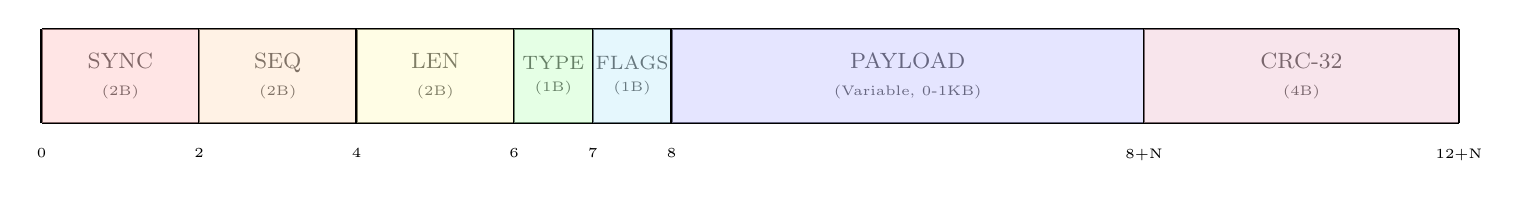
\begin{tikzpicture}[
    font=\small,
    offset/.style={font=\tiny, anchor=north}
]
    % Main frame bar - proportional widths (1 byte = 1 unit for fixed fields)
    \draw[thick] (0,0) -- (18,0);
    \draw[thick] (0,1.2) -- (18,1.2);

    % SYNC (2 bytes = 2 units)
    \draw[thick] (0,0) -- (0,1.2);
    \node[font=\footnotesize, align=center] at (1, 0.6) {SYNC\\{\tiny (2B)}};
    \fill[red!20, opacity=0.5] (0,0) rectangle (2,1.2);

    % SEQ (2 bytes = 2 units)
    \draw[thick] (2,0) -- (2,1.2);
    \node[font=\footnotesize, align=center] at (3, 0.6) {SEQ\\{\tiny (2B)}};
    \fill[orange!20, opacity=0.5] (2,0) rectangle (4,1.2);

    % LEN (2 bytes = 2 units)
    \draw[thick] (4,0) -- (4,1.2);
    \node[font=\footnotesize, align=center] at (5, 0.6) {LEN\\{\tiny (2B)}};
    \fill[yellow!20, opacity=0.5] (4,0) rectangle (6,1.2);

    % TYPE (1 byte = 1 unit)
    \draw[thick] (6,0) -- (6,1.2);
    \node[font=\scriptsize, align=center] at (6.5, 0.6) {TYPE\\{\tiny (1B)}};
    \fill[green!20, opacity=0.5] (6,0) rectangle (7,1.2);

    % FLAGS (1 byte = 1 unit)
    \draw[thick] (7,0) -- (7,1.2);
    \node[font=\scriptsize, align=center] at (7.5, 0.6) {FLAGS\\{\tiny (1B)}};
    \fill[cyan!20, opacity=0.5] (7,0) rectangle (8,1.2);

    % PAYLOAD (variable, 6 units to show it's typically the largest field)
    \draw[thick] (8,0) -- (8,1.2);
    \node[font=\footnotesize, align=center] at (11, 0.6) {PAYLOAD\\{\tiny (Variable, 0-1KB)}};
    \fill[blue!20, opacity=0.5] (8,0) rectangle (14,1.2);

    % CRC-32 (4 bytes = 4 units)
    \draw[thick] (14,0) -- (14,1.2);
    \node[font=\footnotesize, align=center] at (16, 0.6) {CRC-32\\{\tiny (4B)}};
    \fill[purple!20, opacity=0.5] (14,0) rectangle (18,1.2);

    \draw[thick] (18,0) -- (18,1.2);

    % Byte offset labels
    \node[offset] at (0,-0.2) {0};
    \node[offset] at (2,-0.2) {2};
    \node[offset] at (4,-0.2) {4};
    \node[offset] at (6,-0.2) {6};
    \node[offset] at (7,-0.2) {7};
    \node[offset] at (8,-0.2) {8};
    \node[offset] at (14,-0.2) {8+N};
    \node[offset] at (18,-0.2) {12+N};
\end{tikzpicture}%
}

\textbf{System Constraints:}
\begin{itemize}
    \item ESP32-S3-WROOM-1-N16: 16MB flash, 512KB SRAM, NO PSRAM
    \item 100Hz SPI communication (10ms period)
    \item 250Hz motor control loop (4ms period)
    \item Static allocation only (no malloc)
\end{itemize}

\subsubsection{Control Loop Frequency Rationale}

\textbf{Why different loop rates?}

The nested loop architecture follows classic control systems design. The outer loop (SPI at 100Hz) handles command distribution and telemetry collection, while the inner loop (PID at 250Hz) responds quickly to motor dynamics. Running PID at 2.5 times the communication rate ensures smooth control between commands without wasting CPU on excessive computation.

\textbf{Why 250Hz for motor control?}

This is a Nyquist sampling consideration. With DC gearmotors at 210 RPM (3.5 Hz mechanical speed) and a first-order time constant $\tau = 75$ ms (cutoff frequency $f_c = 1/(2\pi \tau) \approx 2.1$ Hz), the 250Hz control rate provides approximately 60 times oversampling of the mechanical dynamics - well above the 2 times Nyquist minimum.

While the ESP32 could easily run the PID loop at 1kHz or higher, doing so would not improve control quality because the motor mechanics are the limiting factor, not the computational speed. The physical system cannot respond faster than its time constant allows. Running at 250Hz balances:

\begin{itemize}
    \item Adequate sampling of motor dynamics (60 times oversampling)
    \item Efficient CPU utilization (4 motors $\times$ PID + encoder reads)
    \item Low latency between velocity commands and motor response
    \item Power efficiency (fewer ADC conversions, GPIO reads, and computations)
\end{itemize}

For context, control loop frequencies should match system dynamics:
\begin{itemize}
    \item DC gearmotors: 50-500 Hz typical
    \item High-speed servos: 1-10 kHz
    \item Motor current control: 10-50 kHz
    \item Temperature control: 0.1-10 Hz
\end{itemize}

\subsection{Key Design Decisions}

\subsubsection{Protocol Stack}
\label{sec:protocol-stack}

\noindent\makebox[\textwidth]{%
\begin{tikzpicture}[
    font=\small,
    node distance = 0cm,
    layer/.style={
        draw,
        thick,
        rectangle,
        minimum width=15cm,
        minimum height=1.3cm,
        align=left,
        text width=14.5cm
    },
]
    \node[layer, fill=red!20] (app) at (0,0) {\textbf{Application} \hfill Motor Commands, Telemetry, OTA Updates};
    \node[layer, fill=orange!20, below=of app] (serial) {\textbf{Serialization} \hfill nanopb (Protocol Buffers) with static allocation};
    \node[layer, fill=yellow!20, below=of serial] (arq) {\textbf{ARQ} \hfill Stop-and-Wait (SEQ/ACK/NACK, 8ms timeout)};
    \node[layer, fill=green!20, below=of arq] (frame) {\textbf{Frame} \hfill SYNC (2B) + Header (6B) + Payload + CRC-32 (4B)};
    \node[layer, fill=blue!20, below=of frame] (transport) {\textbf{Transport} \hfill SPI peripheral mode with DMA (10 Mbps)};
    \draw[->, very thick, gray] (-8, 1) -- (-8, -6) node[midway, left, rotate=90, xshift=-0.5cm, yshift=0.5cm] {Data Flow};
\end{tikzpicture}%
}

\subsubsection{Byte Order and Standards Compliance}

The protocol follows established standards for byte ordering to ensure cross-platform compatibility:

\begin{table}[H]
\centering
\caption{Byte Order Standards by Protocol Field}
\label{tab:byte-order-standards}
\begin{tabular}{|l|l|l|l|}
\hline
\textbf{Field} & \textbf{Byte Order} & \textbf{Standard} & \textbf{Rationale} \\
\hline
SYNC & Big-endian & RFC 1700 & Network byte order for headers \\
SEQ & Big-endian & RFC 1700 & Network byte order for headers \\
LEN & Big-endian & RFC 1700 & Network byte order for headers \\
TYPE & N/A (1 byte) & -- & Single byte, no endianness \\
FLAGS & N/A (1 byte) & -- & Single byte, no endianness \\
CRC-32 & Little-endian & IEEE 802.3 & Standard CRC-32 polynomial \\
\hline
\end{tabular}
\end{table}

\textbf{SYNC Magic Word (0x55AA):} The frame synchronization marker uses the distinctive bit pattern 0x55AA (binary: 0101010101010101 in big-endian wire format). This alternating pattern is easily recognizable and unlikely to appear in random data, making it ideal for frame alignment. The value 0x55AA is transmitted as bytes \texttt{[0x55, 0xAA]} on the wire.

\textbf{RFC 1700 (Network Byte Order):} All multi-byte header fields (SYNC, SEQ, LEN) use big-endian format following RFC 1700 ``Assigned Numbers'' standard. This ensures compatibility when communicating between different architectures (ARM RPi5 and Xtensa ESP32, both little-endian internally).

\textbf{IEEE 802.3 (CRC-32):} The frame checksum uses IEEE 802.3 polynomial (0x04C11DB7) in little-endian format, matching the ESP32 ROM CRC implementation and standard Ethernet CRC libraries. This allows zero-copy CRC validation using hardware accelerators where available.

\vspace{0.2cm}

\noindent\colorbox{keyinsightcolor}{\parbox{\dimexpr\linewidth-2\fboxsep}{%
\textbf{Key Insight:} Mixed byte orders are intentional — headers follow network standards for cross-platform compatibility, while CRC follows IEEE 802.3 for hardware acceleration and library compatibility.
}}

\vspace{0.3cm}

\subsubsection{Memory Budget}

\begin{table}[H]
    \centering
    \begin{minipage}{0.47\textwidth}
        \centering
        \small
        \caption{SRAM Usage (512 KB total)}
        \label{tab:sram-usage}
        {\setlength{\tabcolsep}{3pt}
        \begin{tabular}{lrr}
            \toprule
            \textbf{Component} & \textbf{Size (KB)} & \textbf{Usage (\%)} \\
            \midrule
            DMA double-buffer & 8.0 & 1.56 \\
            RX/TX buffers & 2.0 & 0.39 \\
            Protobuf structs & 1.5 & 0.29 \\
            ARQ state & 4.0 & 0.78 \\
            \midrule
            \textbf{Total} & \textbf{15.5} & \textbf{3.03} \\
            \bottomrule
        \end{tabular}}
    \end{minipage}\hfill%
    \begin{minipage}{0.47\textwidth}
        \centering
        \small
        \caption{Flash Usage (16 MB total)}
        \label{tab:flash-usage}
        {\setlength{\tabcolsep}{3pt}
        \begin{tabular}{lrr}
            \toprule
            \textbf{Component} & \textbf{Size (KB)} & \textbf{Usage (\%)} \\
            \midrule
            Generated protobuf & 80 & 0.49 \\
            Nanopb runtime & 12 & 0.07 \\
            Frame + ARQ layers & 8 & 0.05 \\
            \textbf{} & & \\ % Spacer
            \midrule
            \textbf{Total} & \textbf{100} & \textbf{0.61} \\
            \bottomrule
        \end{tabular}}
    \end{minipage}
\end{table}

\textbf{Memory Budget Calculations:}

\textbf{SRAM (512 KB total):}
\begin{itemize}[leftmargin=*,topsep=2pt,itemsep=1pt]
    \item \textbf{DMA double-buffer:} $2 \times 4092\text{ bytes} = 8184\text{ bytes} = 8.0\text{ KB}$ \\
          \textit{Calculation:} Two ping-pong DMA buffers at \texttt{STAR\_SPI\_DMA\_MAX\_SIZE} (4092 bytes each) \\
          \textit{Usage:} $\frac{8.0}{512} \times 100 = 1.56\%$

    \item \textbf{RX/TX buffers:} $1024 + 1024 = 2048\text{ bytes} = 2.0\text{ KB}$ \\
          \textit{Calculation:} 1 KB RX buffer + 1 KB TX buffer for staging protobuf messages \\
          \textit{Usage:} $\frac{2.0}{512} \times 100 = 0.39\%$

    \item \textbf{Protobuf structs:} $1536\text{ bytes} = 1.5\text{ KB}$ \\
          \textit{Calculation:} Largest message structures (SetVelocityResponse $\approx$ 600 bytes, TelemetryData $\approx$ 400 bytes) \\
          \textit{Usage:} $\frac{1.5}{512} \times 100 = 0.29\%$

    \item \textbf{ARQ state:} $4 + 4 + 8 + 4 + 4092 = 4112\text{ bytes} \approx 4.0\text{ KB}$ \\
          \textit{Calculation:} Sequence number (4B) + retry counter (4B) + timestamp (8B) + state (4B) + retry buffer (4092B) \\
          \textit{Usage:} $\frac{4.0}{512} \times 100 = 0.78\%$

    \item \textbf{Total SRAM:} $8.0 + 2.0 + 1.5 + 4.0 = 15.5\text{ KB}$ \\
          \textit{Total usage:} $\frac{15.5}{512} \times 100 = 3.03\%$
\end{itemize}

\textbf{Flash (16 MB = 16384 KB total):}
\begin{itemize}[leftmargin=*,topsep=2pt,itemsep=1pt]
    \item \textbf{Generated protobuf:} $80\text{ KB}$ \\
          \textit{Calculation:} 6 proto files (common, motor\_control, telemetry, battery\_management, configuration, firmware\_update) $\times$ 13 KB avg compiled size \\
          \textit{Usage:} $\frac{80}{16384} \times 100 = 0.49\%$

    \item \textbf{Nanopb runtime:} $12\text{ KB}$ \\
          \textit{Calculation:} Compiled size of pb\_encode.c, pb\_decode.c, pb\_common.c \\
          \textit{Usage:} $\frac{12}{16384} \times 100 = 0.07\%$

    \item \textbf{Frame + ARQ layers:} $8\text{ KB}$ \\
          \textit{Calculation:} Framing logic + CRC-32 + ARQ state machine + retransmission logic \\
          \textit{Usage:} $\frac{8}{16384} \times 100 = 0.05\%$

    \item \textbf{Total Flash:} $80 + 12 + 8 = 100\text{ KB}$ \\
          \textit{Total usage:} $\frac{100}{16384} \times 100 = 0.61\%$
\end{itemize}

\subsection{Implementation Requirements}

\subsubsection{Protocol Stack Architecture}

The protocol is implemented as a layered stack on both the RPi5 (SPI controller) and ESP32 (SPI peripheral). Each layer has specific responsibilities:

\vspace{0.3cm}

\begin{table}[H]
\centering
\begin{tabular}{|c|l|c|}
\hline
\textbf{Layer} & \textbf{Responsibility} & \textbf{Implementation} \\
\hline
5. Application & Motor commands, telemetry, control logic & Different per platform \\
\hline
4. Protobuf & Message encode/decode (nanopb) & Both sides \\
\hline
3. ARQ & Sequence numbering, ACK/NACK, retry logic & Both sides (symmetric) \\
\hline
2. Framing & Header/footer, CRC-32 verification & Both sides (identical) \\
\hline
1. SPI+DMA & Physical transport with double-buffering & Both sides (different roles) \\
\hline
\end{tabular}
\caption{Protocol stack layers and implementation requirements}
\label{tab:protocol-stack}
\end{table}

\vspace{0.2cm}

\noindent\colorbox{keyinsightcolor}{\parbox{\dimexpr\linewidth-2\fboxsep}{%
\textbf{Key Insight:} Layers 2-4 are nearly identical on both platforms. Only the application layer (Layer 5) and SPI role (Layer 1: controller vs peripheral) differ.
}}

\vspace{0.3cm}

\subsubsection{ESP32 (SPI Peripheral) Implementation}

\vspace{0.2cm}

\noindent\colorbox{layer1color}{\parbox{\dimexpr\linewidth-2\fboxsep}{%
\textbf{Layer 1: SPI Peripheral with DMA}
\vspace{0.1cm}
\begin{itemize}[leftmargin=1.5em,topsep=0pt,itemsep=2pt,parsep=0pt]
    \item Configure SPI3 in peripheral mode using ESP-IDF
    \item Set up DMA with double-buffering: 2 $\times$ 4092 bytes
    \item Register DMA interrupt callbacks for buffer swapping
    \item Wait for chip select from RPi5, respond to clock
\end{itemize}
\vspace{0.05cm}
}}

\vspace{0.25cm}

\noindent\colorbox{layer2color}{\parbox{\dimexpr\linewidth-2\fboxsep}{%
\textbf{Layer 2: Frame Layer (Custom Code)}
\vspace{0.1cm}

\noindent\textit{RX Path:}
\begin{itemize}[leftmargin=1.5em,topsep=0pt,itemsep=2pt,parsep=0pt]
    \item Parse frame header (magic bytes, length, sequence number)
    \item Verify CRC-32 over header + payload
    \item If CRC fails $\rightarrow$ discard packet, send NACK
    \item If CRC valid $\rightarrow$ extract payload, pass to ARQ layer
\end{itemize}

\vspace{0.1cm}
\noindent\textit{TX Path:}
\begin{itemize}[leftmargin=1.5em,topsep=0pt,itemsep=2pt,parsep=0pt]
    \item Build frame: \texttt{[Header | Payload | CRC32 | Footer]}
    \item Calculate CRC-32 over header + payload
    \item Queue complete frame to DMA buffer for transmission
\end{itemize}
\vspace{0.05cm}
}}

\vspace{0.25cm}

\noindent\colorbox{layer3color}{\parbox{\dimexpr\linewidth-2\fboxsep}{%
\textbf{Layer 3: ARQ Layer (Custom Code)}
\vspace{0.1cm}

\noindent\textit{RX Path:}
\begin{itemize}[leftmargin=1.5em,topsep=0pt,itemsep=2pt,parsep=0pt]
    \item Check sequence number against \texttt{last\_acked\_rx}
    \item If duplicate (\texttt{seq} $\leq$ \texttt{last\_acked\_rx}) $\rightarrow$ send ACK, discard payload
    \item If expected (\texttt{seq} = \texttt{last\_acked\_rx} + 1) $\rightarrow$ accept, send ACK
    \item If out-of-order $\rightarrow$ send NACK, request retransmission
\end{itemize}

\vspace{0.1cm}
\noindent\textit{TX Path:}
\begin{itemize}[leftmargin=1.5em,topsep=0pt,itemsep=2pt,parsep=0pt]
    \item Assign \texttt{tx\_sequence\_number} to outgoing frame
    \item Store frame in retry buffer
    \item Start timeout timer (e.g., 10ms)
    \item On timeout $\rightarrow$ retransmit (up to 3 attempts)
    \item On ACK received $\rightarrow$ clear retry buffer, increment \texttt{tx\_seq}
\end{itemize}
\vspace{0.05cm}
}}

\vspace{0.25cm}

\noindent\colorbox{layer4color}{\parbox{\dimexpr\linewidth-2\fboxsep}{%
\textbf{Layer 4: Protobuf (nanopb library)}
\vspace{0.1cm}
\begin{itemize}[leftmargin=1.5em,topsep=0pt,itemsep=2pt,parsep=0pt]
    \item Decode incoming bytes $\rightarrow$ \texttt{SetVelocityRequest}, \texttt{EmergencyStopRequest}
    \item Encode outgoing structs $\rightarrow$ \texttt{SetVelocityResponse}, \texttt{TelemetryData}
    \item Uses \texttt{star.v1} package following Boston Dynamics style guide
    \item Static allocation (no malloc) with \texttt{.options} file constraints
\end{itemize}
\vspace{0.05cm}
}}

\vspace{0.25cm}

\noindent\colorbox{layer5color}{\parbox{\dimexpr\linewidth-2\fboxsep}{%
\textbf{Layer 5: Application}
\vspace{0.1cm}
\begin{itemize}[leftmargin=1.5em,topsep=0pt,itemsep=2pt,parsep=0pt]
    \item Handle motor velocity commands
    \item Read encoder data via multiplexer
    \item Execute PID control loop (250 Hz per motor)
    \item Send telemetry responses (encoder feedback, current, temperature)
\end{itemize}
\vspace{0.05cm}
}}

\vspace{0.4cm}

\subsubsection{RPi5 (SPI Controller) Implementation}

\vspace{0.2cm}

\noindent\colorbox{layer1color}{\parbox{\dimexpr\linewidth-2\fboxsep}{%
\textbf{Layer 1: SPI Controller with DMA}
\vspace{0.1cm}
\begin{itemize}[leftmargin=1.5em,topsep=0pt,itemsep=2pt,parsep=0pt]
    \item Use Linux \texttt{/dev/spidev} interface
    \item Configure SPI3: 10 Mbps, mode 0, 8-bit words
    \item Use \texttt{ioctl(SPI\_IOC\_MESSAGE)} for DMA transfers
    \item Implement userspace double-buffering for continuous operation
\end{itemize}
\vspace{0.05cm}
}}

\vspace{0.25cm}

\noindent\colorbox{layer2color}{\parbox{\dimexpr\linewidth-2\fboxsep}{%
\textbf{Layer 2: Frame Layer} \textit{(Custom Code - SAME AS ESP32)}
\vspace{0.1cm}

\noindent\textit{RX Path:} Parse frame header, verify CRC-32, extract payload or discard on CRC failure

\vspace{0.05cm}
\noindent\textit{TX Path:} Build frame \texttt{[Header | Payload | CRC32 | Footer]}, calculate CRC-32, send via SPI
\vspace{0.05cm}
}}

\vspace{0.25cm}

\noindent\colorbox{layer3color}{\parbox{\dimexpr\linewidth-2\fboxsep}{%
\textbf{Layer 3: ARQ Layer} \textit{(Custom Code - SAME AS ESP32)}
\vspace{0.1cm}

\noindent\textit{RX Path:} Check sequence number, detect duplicates $\rightarrow$ ACK and discard, detect out-of-order $\rightarrow$ NACK

\vspace{0.05cm}
\noindent\textit{TX Path:} Assign sequence number, store in retry buffer, timeout and retry logic, handle ACKs
\vspace{0.05cm}
}}

\vspace{0.25cm}

\noindent\colorbox{layer4color}{\parbox{\dimexpr\linewidth-2\fboxsep}{%
\textbf{Layer 4: Protobuf (Go with protoc-gen-go)}
\vspace{0.1cm}
\begin{itemize}[leftmargin=1.5em,topsep=0pt,itemsep=2pt,parsep=0pt]
    \item Encode: \texttt{SetVelocityRequest}, \texttt{EmergencyStopRequest}
    \item Decode: \texttt{SetVelocityResponse}, \texttt{TelemetryData}, \texttt{EncoderData}
    \item Uses \texttt{star.v1} package following Boston Dynamics style guide
\end{itemize}
\vspace{0.05cm}
}}

\vspace{0.25cm}

\noindent\colorbox{layer5color}{\parbox{\dimexpr\linewidth-2\fboxsep}{%
\textbf{Layer 5: Application (star-gateway)}
\vspace{0.1cm}
\begin{itemize}[leftmargin=1.5em,topsep=0pt,itemsep=2pt,parsep=0pt]
    \item Send motor velocity commands from Nav2 (autonomous) or UI (manual)
    \item All control flows through Nav2 stack for consistent behavior
    \item Receive encoder feedback for odometry calculations
    \item Bridge ROS2 topics to/from ESP32 via SPI
\end{itemize}
\vspace{0.05cm}
}}

\vspace{0.4cm}

\subsubsection{ARQ Symmetry and State Management}

The ARQ layer uses \textbf{Stop-and-Wait} protocol (also called alternating bit protocol). This means each side sends one frame at a time, waits for acknowledgment (ACK) with a timeout, and retries up to 3 times before declaring failure. This approach provides:

\begin{itemize}[leftmargin=1.5em,topsep=4pt,itemsep=2pt]
    \item Simple implementation suitable for embedded systems
    \item Predictable worst-case latency for real-time control
    \item Low memory overhead (single retry buffer, not a window of frames)
    \item Sufficient throughput for 10 Mbps SPI with <1ms frame time
\end{itemize}

The ARQ protocol is \textbf{symmetric} — both sides implement identical Stop-and-Wait logic but maintain separate state for their own transmissions and receptions.

\vspace{0.2cm}
\noindent\textbf{Each Side Maintains:}
\begin{itemize}[leftmargin=1.5em,topsep=4pt,itemsep=4pt]
    \item \textbf{TX sequence number} (\texttt{tx\_seq}): For packets it sends
    \item \textbf{RX last acknowledged} (\texttt{rx\_last\_ack}): For packets it receives
    \item \textbf{Retry buffer}: Stores unacknowledged outgoing packets
    \item \textbf{Timeout timer}: Triggers retransmission if no ACK received
\end{itemize}

\vspace{0.2cm}

\begin{table}[H]
\centering
\begin{tabular}{|l|c|c|}
\hline
\textbf{Responsibility} & \textbf{ESP32 (Peripheral)} & \textbf{RPi5 (Controller)} \\
\hline
Sends & Telemetry, responses & Commands, requests \\
\hline
TX sequence numbering & Own \texttt{tx\_seq} & Own \texttt{tx\_seq} \\
\hline
ACK/NACK generation & Sends ACK for RPi5 & Sends ACK for ESP32 \\
\hline
Retry logic & Retries if no ACK & Retries if no ACK \\
\hline
Duplicate detection & Checks RPi5's \texttt{seq} & Checks ESP32's \texttt{seq} \\
\hline
\end{tabular}
\caption{ARQ role distribution between controller and peripheral}
\label{tab:arq-roles}
\end{table}

\vspace{0.2cm}

\noindent\colorbox{importantcolor}{\parbox{\dimexpr\linewidth-2\fboxsep}{%
\textbf{Important:} The SPI controller/peripheral roles (Layer 1) are \textbf{hardware-level only}. The ARQ layer (Layer 3) treats both sides as equals — each can send, ACK, and retry independently.
}}

\vspace{0.3cm}

\subsubsection{Example Transaction: RPi5 Sends Velocity Command}

\vspace{0.2cm}

\begin{enumerate}[leftmargin=1.5em,topsep=4pt,itemsep=2pt]
    \item \textbf{RPi5 Application:} Create \texttt{SetVelocityRequest} (left=1.0 m/s, right=1.0 m/s)
    \item \textbf{RPi5 Protobuf:} Encode to binary (nanopb)
    \item \textbf{RPi5 ARQ:} Assign \texttt{seq=42}, save to retry buffer, start 10ms timeout
    \item \textbf{RPi5 Frame:} Build packet with header, CRC-32, footer
    \item \textbf{RPi5 SPI:} DMA transfer to ESP32 (controller initiates)
    \item \textbf{ESP32 SPI:} DMA receives packet in double-buffer
    \item \textbf{ESP32 Frame:} Verify CRC-32 $\rightarrow$ valid
    \item \textbf{ESP32 ARQ:} Check \texttt{seq=42} = \texttt{rx\_last\_ack+1} $\rightarrow$ accept
    \item \textbf{ESP32 Protobuf:} Decode to \texttt{SetVelocityRequest} struct
    \item \textbf{ESP32 Application:} Update motor setpoints, execute PID control
    \item \textbf{ESP32 ARQ:} Build ACK packet with \texttt{ack\_seq=42}
    \item \textbf{ESP32 Frame:} Wrap ACK in frame with CRC-32
    \item \textbf{ESP32 SPI:} DMA transmits ACK (peripheral responds)
    \item \textbf{RPi5 SPI:} DMA receives ACK packet
    \item \textbf{RPi5 Frame:} Verify CRC-32 $\rightarrow$ valid
    \item \textbf{RPi5 ARQ:} Got \texttt{ACK(42)} $\rightarrow$ clear retry buffer, cancel timeout
\end{enumerate}

\vspace{0.2cm}

\noindent\textbf{Outcome:} Command successfully delivered with guaranteed delivery via ARQ. If ACK was lost or CRC failed, RPi5 would retransmit after 10ms timeout.

\vspace{0.3cm}

\subsection{ARQ Communication Flow}

\subsubsection{Normal Operation (No Retransmission)}

\begin{figure}[H]
    \centering
    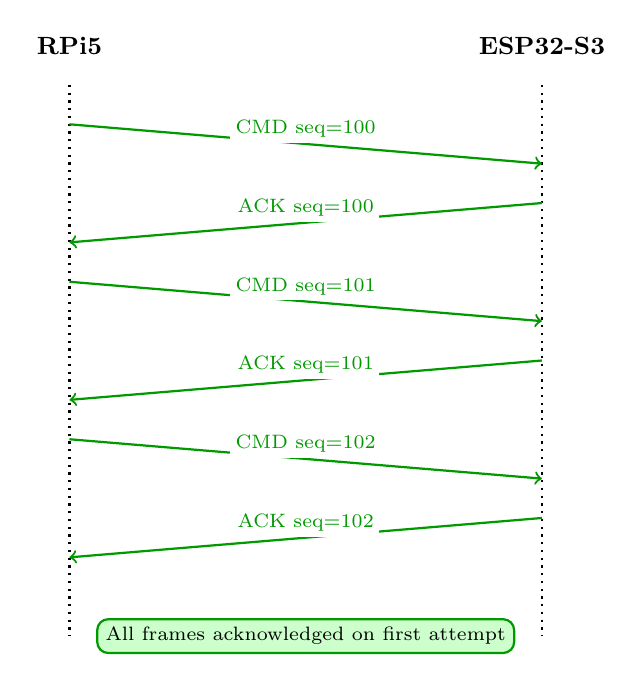
\begin{tikzpicture}[
        node distance=0.8cm,
        entity/.style={font=\small\bfseries},
        success/.style={->, thick, green!60!black},
        msgtext/.style={font=\scriptsize, fill=white, inner sep=2pt}
    ]
        % Entities
        \node[entity] (rpi) at (0, 0) {RPi5};
        \node[entity] (esp) at (6, 0) {ESP32-S3};

        % Vertical timelines
        \draw[thick, dotted] (0, -0.5) -- (0, -7.5);
        \draw[thick, dotted] (6, -0.5) -- (6, -7.5);

        % Transaction 1
        \draw[success] (0, -1) -- node[msgtext, above] {CMD seq=100} (6, -1.5);
        \draw[success] (6, -2) -- node[msgtext, above] {ACK seq=100} (0, -2.5);

        % Transaction 2
        \draw[success] (0, -3) -- node[msgtext, above] {CMD seq=101} (6, -3.5);
        \draw[success] (6, -4) -- node[msgtext, above] {ACK seq=101} (0, -4.5);

        % Transaction 3
        \draw[success] (0, -5) -- node[msgtext, above] {CMD seq=102} (6, -5.5);
        \draw[success] (6, -6) -- node[msgtext, above] {ACK seq=102} (0, -6.5);

        % Success note
        \node[font=\scriptsize, fill=green!20, draw=green!60!black, thick, rounded corners, inner sep=3pt] at (3, -7.5) {All frames acknowledged on first attempt};
    \end{tikzpicture}
    \caption{Normal ARQ Flow - Three Successful Transactions}
\end{figure}

\subsubsection{Error Recovery Scenarios}

\begin{figure}[H]
    \centering
    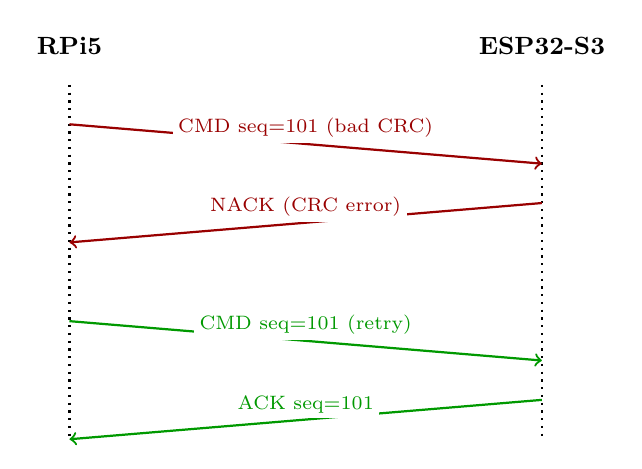
\begin{tikzpicture}[
        node distance=0.8cm,
        entity/.style={font=\small\bfseries},
        success/.style={->, thick, green!60!black},
        error/.style={->, thick, red!60!black},
        msgtext/.style={font=\scriptsize, fill=white, inner sep=2pt}
    ]
        % Entities
        \node[entity] (rpi) at (0, 0) {RPi5};
        \node[entity] (esp) at (6, 0) {ESP32-S3};

        % Vertical timelines
        \draw[thick, dotted] (0, -0.5) -- (0, -5);
        \draw[thick, dotted] (6, -0.5) -- (6, -5);

        % CRC error scenario
        \draw[error] (0, -1) -- node[msgtext, above] {CMD seq=101 (bad CRC)} (6, -1.5);
        \draw[error] (6, -2) -- node[msgtext, above] {NACK (CRC error)} (0, -2.5);
        \draw[success] (0, -3.5) -- node[msgtext, above] {CMD seq=101 (retry)} (6, -4);
        \draw[success] (6, -4.5) -- node[msgtext, above] {ACK seq=101} (0, -5);
    \end{tikzpicture}
    \caption{CRC Error - Retry with Same Sequence Number}
\end{figure}

\begin{figure}[H]
    \centering
    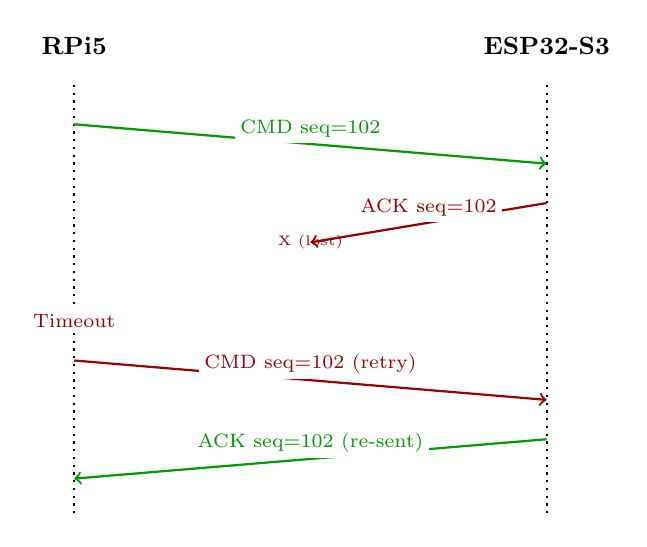
\begin{tikzpicture}[
        node distance=0.8cm,
        entity/.style={font=\small\bfseries},
        msg/.style={->, thick},
        success/.style={->, thick, green!60!black},
        error/.style={->, thick, red!60!black},
        msgtext/.style={font=\scriptsize, fill=white, inner sep=2pt}
    ]
        % Entities and timelines
        \node[entity] (rpi) at (0, 0) {RPi5};
        \node[entity] (esp) at (6, 0) {ESP32-S3};
        \draw[thick, dotted] (0, -0.5) -- (0, -6);
        \draw[thick, dotted] (6, -0.5) -- (6, -6);

        % Diagram
        \draw[success] (0, -1) -- node[msgtext, above] {CMD seq=102} (6, -1.5);
        \draw[error] (6, -2) -- node[msgtext, above] {ACK seq=102} (3, -2.5);
        \node[font=\tiny, red!60!black] at (3, -2.5) {X (lost)};
        \draw[dashed, error] (0, -3.5) -- node[msgtext] {Timeout} (0, -3.5);
        \draw[error] (0, -4) -- node[msgtext, above] {CMD seq=102 (retry)} (6, -4.5);
        \draw[success] (6, -5) -- node[msgtext, above] {ACK seq=102 (re-sent)} (0, -5.5);
    \end{tikzpicture}
    \caption{Duplicate Packet Scenario (Lost ACK)}
\end{figure}

\begin{figure}[H]
    \centering
    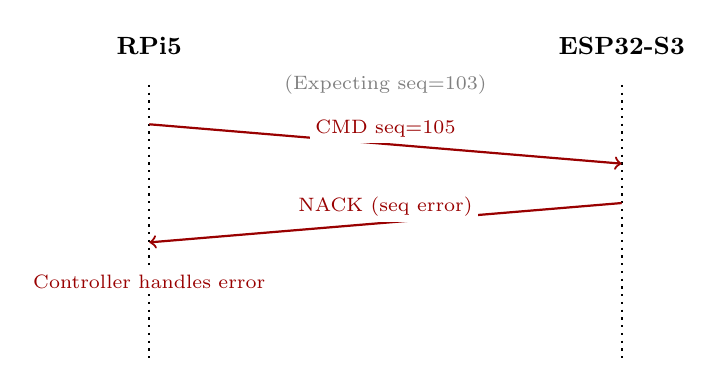
\begin{tikzpicture}[
        node distance=0.8cm,
        entity/.style={font=\small\bfseries},
        msg/.style={->, thick},
        success/.style={->, thick, green!60!black},
        error/.style={->, thick, red!60!black},
        msgtext/.style={font=\scriptsize, fill=white, inner sep=2pt}
    ]
        % Entities and timelines
        \node[entity] (rpi) at (0, 0) {RPi5};
        \node[entity] (esp) at (6, 0) {ESP32-S3};
        \draw[thick, dotted] (0, -0.5) -- (0, -4);
        \draw[thick, dotted] (6, -0.5) -- (6, -4);

        % Diagram
        \node[font=\scriptsize, gray] at (3, -0.5) {(Expecting seq=103)};
        \draw[error] (0, -1) -- node[msgtext, above] {CMD seq=105} (6, -1.5);
        \draw[error] (6, -2) -- node[msgtext, above] {NACK (seq error)} (0, -2.5);
        \draw[dashed, error] (0, -3) -- node[msgtext] {Controller handles error} (0, -3);
    \end{tikzpicture}
    \caption{Out-of-Order Packet Scenario}
\end{figure}

\begin{figure}[H]
    \centering
    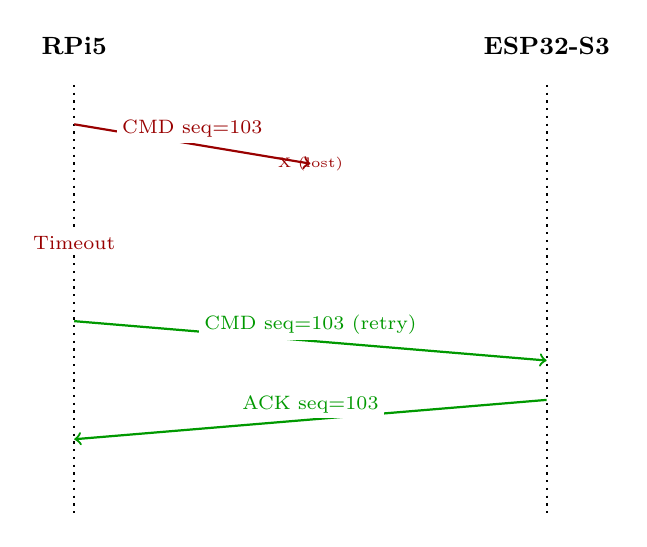
\begin{tikzpicture}[
        node distance=0.8cm,
        entity/.style={font=\small\bfseries},
        msg/.style={->, thick},
        success/.style={->, thick, green!60!black},
        error/.style={->, thick, red!60!black},
        msgtext/.style={font=\scriptsize, fill=white, inner sep=2pt}
    ]
        % Entities and timelines
        \node[entity] (rpi) at (0, 0) {RPi5};
        \node[entity] (esp) at (6, 0) {ESP32-S3};
        \draw[thick, dotted] (0, -0.5) -- (0, -6);
        \draw[thick, dotted] (6, -0.5) -- (6, -6);

        % Diagram
        \draw[error] (0, -1) -- node[msgtext, above] {CMD seq=103} (3, -1.5);
        \node[font=\tiny, red!60!black] at (3, -1.5) {X (lost)};
        \draw[dashed, error] (0, -2.5) -- node[msgtext] {Timeout} (0, -2.5);
        \draw[success] (0, -3.5) -- node[msgtext, above] {CMD seq=103 (retry)} (6, -4);
        \draw[success] (6, -4.5) -- node[msgtext, above] {ACK seq=103} (0, -5);
    \end{tikzpicture}
    \caption{Lost Packet Scenario (Timeout)}
\end{figure}


\subsection{Error Handling Strategies}

\begin{center}
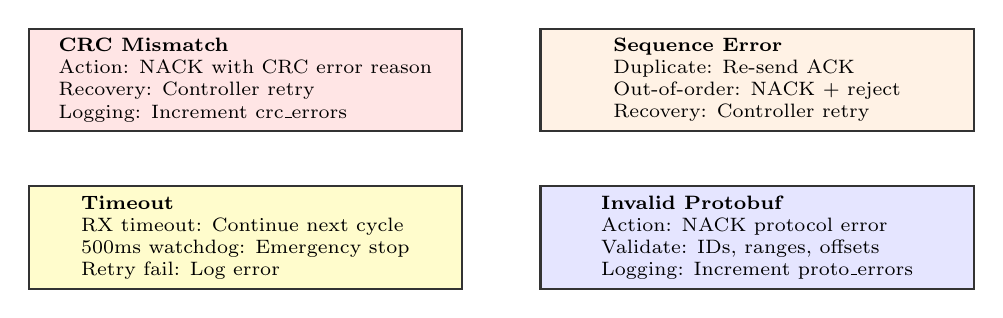
\begin{tikzpicture}[
    errorbox/.style={rectangle, draw=black!80, thick, fill=red!10, minimum width=5.5cm, minimum height=1.3cm, font=\scriptsize, align=left},
    title/.style={font=\small\bfseries}
]
    % CRC Mismatch
    \node[errorbox] (crc) at (0, 0) {
        \textbf{CRC Mismatch}\\
        Action: NACK with CRC error reason\\
        Recovery: Controller retry\\
        Logging: Increment crc\_errors
    };

    % Sequence Error
    \node[errorbox, fill=orange!10] (seq) at (6.5, 0) {
        \textbf{Sequence Error}\\
        Duplicate: Re-send ACK\\
        Out-of-order: NACK + reject\\
        Recovery: Controller retry
    };

    % Timeout
    \node[errorbox, fill=yellow!20] (timeout) at (0, -2) {
        \textbf{Timeout}\\
        RX timeout: Continue next cycle\\
        500ms watchdog: Emergency stop\\
        Retry fail: Log error
    };

    % Invalid Protobuf
    \node[errorbox, fill=blue!10] (proto) at (6.5, -2) {
        \textbf{Invalid Protobuf}\\
        Action: NACK protocol error\\
        Validate: IDs, ranges, offsets\\
        Logging: Increment proto\_errors
    };
\end{tikzpicture}
\end{center}



% Section 2: Protocol Buffer Schema Definitions
% =============================================================================
% PROTOCOL BUFFER SCHEMAS
% =============================================================================

\newpage
\section{Protocol Buffer Schema Architecture}

This section documents the Protocol Buffer schema architecture for RPi5$\leftrightarrow$RX72N communication. All schemas follow the \textbf{Boston Dynamics Protobuf Style Guide
} for
  consistency, maintainability,
      and industry best practices.

\subsection{Architecture Overview
 }

\textbf{Overview:} Five gRPC services define the complete API surface for robot control, organized by functional domain. Services communicate via the nanopb-serialized frames described in Section 1.

\noindent\makebox[\textwidth]{
  %
\begin{tikzpicture}[font =\small, node distance=0.4cm,
                     service/.style={draw, thick, rectangle,
                                        minimum width = 6cm,
                                        minimum height = 1.1cm, align = center},
                     common/.style={draw, thick, rectangle,
                                       minimum width = 14cm,
                                       minimum height = 1.1cm, align = center,
                                       fill=cyan!20},
  ] % Left column - Core Services
    \node[service, fill=blue!20](motor) at(-4, 0){\textbf{MotorControlService}\\Velocity commands, encoder streaming};
  \node[service, fill=green!20, below=of motor](telemetry){\textbf{TelemetryService}\\Sensor data, system status};

  % Right column - Support Services
    \node[service, fill=orange!20](battery) at(4, 0){\textbf{BatteryManagementService}\\BMS state, protection, balancing};
  \node[service, fill=yellow!20, below=of battery](config){\textbf{ConfigurationService}\\PID gains, calibration, NVS};

  % Common proto spans bottom
    \node[common, below=0.8cm of telemetry, xshift=4cm](common){\textbf{common.proto}\\Headers, status codes, geometry types};

  % Labels
    \node[above=0.3cm of motor, font=\footnotesize\bfseries]{Real-Time Control};
  \node[above=0.3cm of battery, font=\footnotesize\bfseries]{Device Management};

  % Arrows to common - routed around blocks
    \draw[->, thick, gray](motor.west)-- ++(-0.5, 0) |-(common.west);
  \draw[->, thick, gray](telemetry.south)--(telemetry.south |-common.north);
  \draw[->, thick, gray](battery.east)-- ++(0.5, 0) |-(common.east);
  \draw[->, thick, gray](config.south)--(config.south |-common.north);
  \end{tikzpicture} %
}

\vspace{0.3cm}

\layerbox{keyinsightcolor} { Key Design Principles}
{
  %
\begin{itemize}[leftmargin = 1.5em, topsep = 2pt, itemsep = 1pt]
    \item \textbf{Versioned Package :} All services use \texttt {
    star.v1
 } namespace for API evolution
    \item \textbf{Request/Response Headers:} Every RPC includes tracing, timestamps, and status
    \item \textbf{Streaming Support:} Continuous data uses server streaming (up to 100Hz)
    \item \textbf{Static Allocation:} All messages sized for nanopb constraints (no dynamic memory)
\end{itemize}
}

\textbf{Note:} Naming conventions, unit suffixes, and coding standards are consolidated in Section~\ref{sec:protobuf-style} (Style Guide and Conventions).

\subsection{Service Specifications}
\label{sec:service-specifications}

\subsubsection{MotorControlService}

\textbf{Purpose:} Low-latency differential drive control with real-time encoder feedback.

\textbf{Target Latency:} $<$10ms round-trip for velocity commands.

\begin{table}[H]
\centering
\caption{MotorControlService RPCs}
\label{tab:motor-rpcs}
\begin{tabular} { | l | l | p{6cm} |}
\hline
\textbf{RPC} & \textbf{Type} & \textbf{Description}
\\
\hline SetVelocity &Unary &Set left /
    right wheel velocities(m / s) \\
EmergencyStop &Unary &Immediate stop,
    priority over all commands \\
SetMotorPower &Unary &Direct PWM
        control(bypass PID, testing only) \\
StreamEncoders &Server
        stream &Encoder ticks and velocity at 1 -
        100Hz \\
ControlStream &Bidirectional &Velocity in,
    encoder feedback out \\
\hline
\end{tabular}
\end{table}

\textbf{Key Messages:}
\begin{itemize}[leftmargin = 1.5em, topsep = 4pt, itemsep = 2pt]
    \item \texttt {
  VelocityCommand
}
--Left / right velocity(m / s), sequence number, timestamp
    \item \texttt {
  EncoderData
}
--Motor ID, tick count(341.2 PPR), velocity, timestamp
    \item \texttt {
  MotorStatus
}
--Duty cycle, velocity, temperature, current, fault flags
    \item \texttt {
  PidConfig
}
--Kp, Ki, Kd gains with output saturation limits
\end{itemize}

\subsubsection{TelemetryService}

\textbf{Purpose :} Real -
    time sensor data aggregation and system health monitoring.

\begin{table}[H]
\centering
\caption{TelemetryService RPCs}
\label{tab:telemetry-rpcs}
\begin{tabular} { | l | l | p{6cm} |}
\hline
\textbf{RPC} & \textbf{Type} & \textbf{Description}
\\
\hline GetTelemetry &Unary &Snapshot of all sensor
        data \\
StreamTelemetry &Server stream &Continuous sensor updates at 1 -
    100Hz \\
GetSystemStatus &Unary &Firmware version,
    uptime, connection states \\
\hline
\end{tabular}
\end{table}

\textbf{Key Messages:}
\begin{itemize}[leftmargin = 1.5em, topsep = 4pt, itemsep = 2pt]
    \item \texttt {
  TelemetryData
}
--IMU, GPS, battery \%, WiFi signal, CPU usage, temperature
    \item \texttt {
  ImuData
}
--Pitch / roll / yaw(rad), acceleration(m / s$ ^ 2 $), angular velocity(rad / s)
    \item \texttt {
  GpsData
}
--Lat / lon(degrees), altitude(m), accuracy, satellite count, fix type
    \item \texttt {
  SystemStatus
}
--Connection states, operating mode, free heap, uptime
\end{itemize}

\textbf{Enumerations:
}
\begin{itemize}[leftmargin = 1.5em, topsep = 4pt, itemsep = 2pt]
    \item \texttt {
  RobotMode
}
--IDLE, MANUAL, AUTONOMOUS, MAPPING, EMERGENCY\_STOP
    \item \texttt {
  ConnectionStatus
}
--CONNECTED, DISCONNECTED, CONNECTING, ERROR
    \item \texttt { GpsFix}
--NONE, 2D, 3D, DGPS, RTK\_FLOAT, RTK\_FIXED
\end{itemize}

\subsubsection{BatteryManagementService}

\textbf{Purpose:} BQ7850 BMS monitoring for lithium-ion battery pack safety and management.

\textbf{Hardware:} TI BQ7850 16-cell BMS with I2C interface.

\begin{table}[H]
\centering
\caption{BatteryManagementService RPCs}
\label{tab:battery-rpcs}
\begin{tabular} { | l | l | p{6cm} |}
\hline
\textbf{RPC} & \textbf{Type} & \textbf{Description}
\\
\hline GetBatteryState &Unary &Complete battery snapshot(
    cells, temps, SOC) \\
StreamBatteryState &Server stream &Continuous battery
        monitoring \\
Get
        / SetProtectionThresholds &Unary &OV / UV / OC
        / OT protection limits \\
Enable / DisableCellBalancing &Unary &Per
    - cell passive balancing control \\
ControlFets &Unary &Charge
          / discharge FET enable / disable \\
GetDeviceInfo &Unary &Manufacturer,
    serial, chemistry, versions \\
\hline
\end{tabular}
\end{table}

\textbf{Key Messages:}
\begin{itemize}[leftmargin = 1.5em, topsep = 4pt, itemsep = 2pt]
    \item \texttt {
  BatteryState
}
--Composite of all battery data
    \item \texttt { CellData}
--Individual cell voltages(mV), pack voltage, valid cell count
    \item \texttt {
  BatteryTemperatureData
}
--Thermistor readings(0.1\textdegree C), average
    \item \texttt {
  StateOfChargeData
}
--Relative / absolute SOC(\%), capacity(mAh), cycle count
    \item \texttt {
  ProtectionThresholds
}
--OV / UV voltage limits, OC current limits, OT temperatures
\end{itemize}

\subsubsection{ConfigurationService}

\textbf{Purpose :
} Runtime parameter management with NVS persistence across power cycles.

\begin{table}[H]
\centering
\caption{ConfigurationService RPCs}
\label{tab:config-rpcs}
\begin{tabular} { | l | l | p{6cm} |}
\hline
\textbf{RPC} & \textbf{Type} & \textbf{Description}
\\
\hline GetConfiguration &Unary &
        Read current system configuration \\
SetConfiguration &Unary &Apply
        configuration(optional NVS persist) \\
ResetToDefaults &Unary &Restore
    factory defaults \\
ValidateConfiguration &Unary &Validate without
    applying \\
SaveConfiguration &Unary &Persist in
    - memory config to NVS \\
Get / SetMotorPidConfig &Unary &Per
    - motor PID tuning \\
\hline
\end{tabular}
\end{table}

\textbf{Key Messages:}
\begin{itemize}[leftmargin = 1.5em, topsep = 4pt, itemsep = 2pt]
    \item \texttt {
  SystemConfiguration
}
--Complete config with version and CRC32
    \item \texttt { MotorPidConfig}
--Per - motor PID gains(4 motors supported)
    \item \texttt {
  CurrentSensorCalibration
} -- Offset and scale for current sensing
    \item \texttt{SafetyThresholds}
--Overcurrent, thermal shutdown, cell imbalance limits
    \item \texttt {
  TimingConfig
}
--Motor period, telemetry period, communication timeout
\end{itemize}

\subsection{common.proto-- Shared Types}

All services import \texttt {
  common.proto
} for
  standardized request / response handling.

\begin{table}[H]
\centering
\caption{Standard Headers}
\label{tab:headers}
\begin{tabular} { | l | p{9cm} |}
\hline
\textbf{Message} & \textbf{Fields}
\\
\hline RequestHeader &request\_id(UUID), client\_timestamp, client\_version,
    timeout \\
ResponseHeader &request\_id(echo), server\_timestamp, status,
    error \_message, latency\_us \\
\hline
\end{tabular}
\end{table}

\textbf{Status Codes :} UNKNOWN, OK, INVALID\_REQUEST, INTERNAL\_ERROR,
    NOT\_FOUND, TIMEOUT, INVALID\_STATE,
    ESTOP\_ACTIVE

\textbf{Geometric Types:
}
\begin{itemize}[leftmargin = 1.5em, topsep = 4pt, itemsep = 2pt]
    \item \texttt {
  Vector3
}
--Generic 3D vector(x, y, z)
    \item \texttt { Quaternion}
--Orientation(w, x, y, z)
    \item \texttt { SE2Pose}
--2D pose(x\_m, y\_m, angle\_rad)
    \item \texttt { SE2Velocity}
--2D velocity(vx\_mps, vy\_mps, omega\_rad\_per\_s)
\end{itemize}

\subsection{Code Generation and Integration}

\begin{table}[H]
\centering
\caption{Code Generation Targets}
\label{tab:codegen}
\begin{tabular}{|l|l|l|l|}
\hline
\textbf{Target} & \textbf{Generator} & \textbf{Output} & \textbf{Usage} \\
\hline
Go & protoc-gen-go + grpc & \texttt{gen/go/} & star-gateway(RPi5) \\
\hline
nanopb & nanopb\_generator & \texttt{gen/nanopb/} & RX72N firmware \\
\hline
\end{tabular}
\end{table}

\textbf{nanopb Constraints:} RX72N requires static allocation. Field sizes are configured in \texttt{.options} files:
\begin{itemize}[leftmargin=1.5em,topsep=4pt,itemsep=2pt]
    \item String fields: \texttt{max\_size:64} (request\_id), \texttt{max\_size:128} (error\_message)
    \item Repeated fields: \texttt{max\_count:16} (cell voltages), \texttt{max\_count:4} (motors)
    \item Bytes fields: \texttt{max\_size:1024} (firmware chunks)
\end{itemize}

\textbf{Build Integration:}
\begin{itemize}[leftmargin = 1.5em, topsep = 4pt, itemsep = 2pt]
    \item \textbf{Linting:
}
\texttt{buf lint} enforces style guide compliance
    \item \textbf{Breaking Changes:
}
\texttt{buf breaking} detects API incompatibilities
    \item \textbf{CI Pipeline :} Automatic generation and testing on PR
\end{itemize}


% Section 3: Hardware Pin Connections
% =============================================================================
% HARDWARE PIN CONNECTIONS
% =============================================================================

\newpage
\section{Hardware Pin Connections}

\subsection{RX72N Microcontroller Pinout (R5F572NNHGFP\#30)}

\begin{longtable}{|c|l|l|p{5cm}|}
\hline
\textbf{Pin} & \textbf{Pin Name} & \textbf{Connected To} & \textbf{Note/Comment} \\
\hline
\endfirsthead

\hline
\textbf{Pin} & \textbf{Pin Name} & \textbf{Connected To} & \textbf{Note/Comment} \\
\hline
\endhead

\hline
\multicolumn{4}{r}{\textit{Continued on next page}} \\
\endfoot

\hline
\endlastfoot

1 & AVCC1 & Bypass caps & \\
\hline
2 & EMLE & Emulator Configuration jumper & See Table~\ref{tab:emulator-config} \\
\hline
3 & AVSS1 & Ground & \\
\hline
4 & PJ3 & & \\
\hline
5 & VCL & 220nF cap to ground & \\
\hline
6 & VBATT & Boards 3v3 & \\
\hline
7 & MD/FINED & E1E2-Emulator-Interface, DIP switch & See Table~\ref{tab:op-mode-config}. Default: OFF,OFF \\
\hline
8 & XCIN & 10k resistor to ground & RTC crystal input (not used) \\
\hline
9 & XCOUT & Floating & Left floating per datasheet \\
\hline
10 & RES\# & E1E2-Emulator-Interface, Reset button & MCU reset \\
\hline
11 & P37/XTAL & 24MHz crystal (to pin 13) & System clock crystal \\
\hline
12 & VSS & Ground & \\
\hline
13 & P36/EXTAL & 24MHz crystal (to pin 11) & System clock crystal \\
\hline
14 & VCC & Boards 3v3 & \\
\hline
15 & P35/NMI/UPSEL & UPSEL configuration jumper & Can be used for NMI (not currently used). See Table~\ref{tab:upsel-config} \\
\hline
16 & P34/TST\# & E1E2-Emulator-Interface & \\
\hline
17 & P33 & RES\#, CY7C65213A-28PVXI & USB to UART IC for flashing (resets system before firmware flash). See Table~\ref{tab:reset-pin-states} \\
\hline
18 & & & \\
\hline
19 & P31/TMS & E1E2-Emulator-Interface & \\
\hline
20 & P30/TDI & E1E2-Emulator-Interface & \\
\hline
21 & P27/TCK & E1E2-Emulator-Interface & \\
\hline
22 & P26/TDO & E1E2-Emulator-Interface & \\
\hline
23 & & & \\
\hline
24 & & & \\
\hline
25 & & & \\
\hline
26 & & & \\
\hline
27 & & & \\
\hline
28 & & & \\
\hline
29 & & & \\
\hline
30 & P16/USB0\_VBUS & USB0 VBUS & \\
\hline
31 & & & \\
\hline
32 & & & \\
\hline
33 & & & \\
\hline
34 & & & \\
\hline
35 & VCC\_USB & Boards 3v3 & \\
\hline
36 & USB0\_DM & USB0 DN (27R resistor) & \\
\hline
37 & USB0\_DP & USB0 DP (27R resistor) & \\
\hline
38 & VSS\_USB & Ground & \\
\hline
39 & & & \\
\hline
40 & & & \\
\hline
41 & & & \\
\hline
42 & & & \\
\hline
43 & & & \\
\hline
44 & & & \\
\hline
45 & PC7/UB & E1E2-Emulator-Interface, DIP switch & Operation mode configuration. See Table~\ref{tab:op-mode-config} \\
\hline
46 & & & \\
\hline
47 & & & \\
\hline
48 & & & \\
\hline
49 & & & \\
\hline
50 & & & \\
\hline
51 & & & \\
\hline
52 & & & \\
\hline
53 & PB7/TXD9 & Debug SCI USB-C RX & UART crossed. See Table~\ref{tab:sci9-config} \\
\hline
54 & PB6/RXD9 & Debug SCI USB-C TX & UART crossed. See Table~\ref{tab:sci9-config} \\
\hline
55 & & & \\
\hline
56 & & & \\
\hline
57 & & & \\
\hline
58 & & & \\
\hline
59 & & & \\
\hline
60 & VCC & Boards 3v3 & \\
\hline
61 & & & \\
\hline
62 & VSS & Ground & \\
\hline
63 & & & \\
\hline
64 & & & \\
\hline
65 & & & \\
\hline
66 & & & \\
\hline
67 & & & \\
\hline
68 & & & \\
\hline
69 & & & \\
\hline
70 & & & \\
\hline
71 & & & \\
\hline
72 & & & \\
\hline
73 & & & \\
\hline
74 & & & \\
\hline
75 & & & \\
\hline
76 & & & \\
\hline
77 & & & \\
\hline
78 & & & \\
\hline
79 & & & \\
\hline
80 & & & \\
\hline
81 & & & \\
\hline
82 & & & \\
\hline
83 & & & \\
\hline
84 & & & \\
\hline
85 & & & \\
\hline
86 & & & \\
\hline
87 & & & \\
\hline
88 & & & \\
\hline
89 & & & \\
\hline
90 & & & \\
\hline
91 & & & \\
\hline
92 & & & \\
\hline
93 & & & \\
\hline
94 & & & \\
\hline
95 & & & \\
\hline
96 & & & \\
\hline
97 & & & \\
\hline
98 & & & \\
\hline
99 & & & \\
\hline
100 & & & \\
\hline
\end{longtable}

\begin{table}[H]
\centering
\caption{Emulator Configuration Jumper Settings}
\label{tab:emulator-config}
\begin{tabular}{|p{6cm}|p{8cm}|}
\hline
\textbf{Jumper Position} & \textbf{Configuration} \\
\hline
Shorted Pin 1-2 (normal Operation) & E1/E2 Lite normal debugging (use this mode for normal operation). Microcontroller single operation (without emulator) \\
\hline
Shorted Pin 2-3 (debug with E1/E2) & E1/E2 Lite debugging with Hot plug-in \\
\hline
All open & DO NOT SET \\
\hline
\end{tabular}
\end{table}

\begin{table}[H]
\centering
\caption{Operation Configuration Mode DIP Switch Settings}
\label{tab:op-mode-config}
\small
\textbf{Note:} There are 2 USB-C ports. To flash we can use the SCI boot mode if we want to flash with the SCI USB-C. To flash we can use the USB0 boot mode if we want to flash with the USB0 USB-C.

\vspace{0.2cm}

\begin{tabular}{|c|c|c|l|}
\hline
\textbf{Pin1} & \textbf{Pin2} & \textbf{UPSEL\_CFG} & \textbf{OP Mode} \\
\hline
OFF & X & X & Single Chip Mode \\
\hline
ON & OFF & X & SCI Boot Mode (SCI1) \\
\hline
ON & ON & 1/2 & USB (Bus Powered) (USB0) \\
\hline
ON & ON & 2/3 & USB (Self Powered) (USB0) \\
\hline
\end{tabular}
\end{table}

\begin{table}[H]
\centering
\caption{UPSEL Power Configuration for USB Boot Mode}
\label{tab:upsel-config}
\begin{tabular}{|l|l|}
\hline
\textbf{Jumper Position} & \textbf{Power Configuration for USB Boot Mode} \\
\hline
Shorted Pin 1-2 (No battery pack) & Bus Powered \\
\hline
Shorted Pin 2-3 (Battery Pack) & Self Powered \\
\hline
\end{tabular}
\end{table}

\begin{table}[H]
\centering
\caption{Required Pin States Upon Reset Release}
\label{tab:reset-pin-states}
\small
To enter a mode capable of flashing firmware, the following pin configurations must be held when the \textbf{RES\# pin} goes from Low to High:

\vspace{0.2cm}

\begin{tabular}{|l|l|l|l|}
\hline
\textbf{Desired Flashing Mode} & \textbf{MD Pin Level} & \textbf{UB Pin Level} & \textbf{Interface Used} \\
\hline
Boot Mode (SCI) & Low & Low & Serial (SCI1) \\
\hline
Boot Mode (USB) & Low & High & USB \\
\hline
Boot Mode (FINE) & Low $\rightarrow$ High* & Low & FINE Interface \\
\hline
\end{tabular}

\vspace{0.2cm}

\small
*For FINE interface, the MD pin must be Low at reset release and then switched to High within 20 to 100 ms.
\end{table}

\begin{table}[H]
\centering
\caption{SCI9 Firmware Configuration (MPC Settings)}
\label{tab:sci9-config}
\small
\textbf{Note:} Pins are multiplexed. Firmware must explicitly configure the Multi-Function Pin Controller (MPC) as follows:

\vspace{0.2cm}

\begin{tabular}{|l|p{11cm}|}
\hline
\textbf{Step} & \textbf{Configuration} \\
\hline
1. UNLOCK MPC & Unlock registers using the Write-Protect Register (PWPR) \\
\hline
2. PIN FUNCTION SELECT & \textbf{PIN 53 (PB7) $\rightarrow$ TXD9:} Set PB7PFS.PSEL[5:0] = 001010b (0x0A) \newline \textbf{PIN 54 (PB6) $\rightarrow$ RXD9:} Set PB6PFS.PSEL[5:0] = 001010b (0x0A) \\
\hline
3. ENABLE PERIPHERAL & Set Port Mode Register (PMR) bit to '1' for both PB7 and PB6 \\
\hline
\end{tabular}

\vspace{0.2cm}

\small
\textbf{USB-UART IC Configuration:} Use Cypress configuration utility to enable BUSDETECT.
\end{table}

\subsection{Raspberry Pi 5 Pinout}

\textbf{Status:} Pin assignments are pending hardware verification and will be documented once validated.

\subsection{Additional Peripheral Connections}

\textbf{Status:} Peripheral connections are pending hardware verification and will be documented once validated.


% Section 12: End-to-End Communication Stack
% =============================================================================
% END-TO-END COMMUNICATION STACK
% =============================================================================

\newpage
\section{End-to-End Communication Stack}
\label{sec:communication-stack}

\subsection{Overview}

The STAR communication stack connects the user interface through a layered architecture down to the RX72N motor controller. Each layer serves a distinct purpose: the UI provides human interaction, the gateway bridges high-level commands to the robot control framework, ROS2 handles autonomous navigation and sensor fusion, and the frame protocol delivers serialized messages over either USB CDC or SPI to the real-time firmware.

\vspace{0.3cm}

\noindent\makebox[\textwidth]{%
\begin{tikzpicture}[
    font=\small,
    node distance=0.4cm,
    box/.style={
        draw,
        thick,
        rectangle,
        minimum height=1.1cm,
        align=center,
        rounded corners=2pt
    },
    arrow/.style={->, thick, >=stealth}
]
    % UI
    \node[box, fill=blue!15, minimum width=2.4cm] (ui) at (0,0) {UI\\{\tiny TypeScript}};

    % Gateway
    \node[box, fill=orange!20, minimum width=2.6cm, right=of ui] (gw) {Gateway\\{\tiny Go, :8080}};

    % ROS2 Bridge
    \node[box, fill=green!15, minimum width=2.6cm, right=of gw] (ros2) {ROS2 Bridge\\{\tiny C++}};

    % Gateway Services
    \node[box, fill=orange!20, minimum width=2.6cm, right=of ros2] (svc) {Gateway\\Services};

    % Frame Protocol
    \node[box, fill=yellow!20, minimum width=2.4cm, right=of svc] (frame) {Frame\\Protocol};

    % Transport
    \node[box, fill=cyan!15, minimum width=2.4cm, below=0.8cm of frame] (transport) {Transport\\{\tiny USB CDC / SPI}};

    % RX72N
    \node[box, fill=red!15, minimum width=2.6cm, below=0.8cm of transport] (rx72n) {RX72N\\{\tiny C, ThreadX}};

    % Motor Control
    \node[box, fill=purple!15, minimum width=2.4cm, left=of rx72n] (motor) {Motor\\Control};

    % Arrows with labels
    \draw[arrow] (ui) -- node[above, font=\tiny] {WebSocket} node[below, font=\tiny] {JSON} (gw);
    \draw[arrow] (gw) -- node[above, font=\tiny] {gRPC} node[below, font=\tiny] {protobuf} (ros2);
    \draw[arrow] (ros2) -- node[above, font=\tiny] {gRPC} (svc);
    \draw[arrow] (svc) -- node[above, font=\tiny] {proto.Marshal} (frame);
    \draw[arrow] (frame) -- node[right, font=\tiny] {SYNC+CRC} (transport);
    \draw[arrow] (transport) -- node[right, font=\tiny] {Physical} (rx72n);
    \draw[arrow] (rx72n) -- node[above, font=\tiny] {PID + PWM} (motor);
\end{tikzpicture}%
}

\vspace{0.3cm}

\noindent\colorbox{keyinsightcolor}{\parbox{\dimexpr\linewidth-2\fboxsep}{%
\textbf{Key Insight:} All control paths (autonomous Nav2 and manual UI) converge at the gateway, ensuring a single serialization and transport layer regardless of command source. The RX72N firmware is transport-agnostic --- it processes identical frames whether they arrive over USB CDC or SPI.
}}

\subsection{Transport Priority}

USB CDC is the \textbf{primary} transport and SPI is the \textbf{backup}. Priority values are defined in \texttt{star-gateway/internal/manager/types.go}:

\begin{lstlisting}[language=Go, caption={Transport Priority Constants}]
PriorityUSB = 10  // higher = preferred
PrioritySPI = 5
\end{lstlisting}

The \texttt{TransportManager} selects the highest-priority healthy transport at runtime. USB is preferred for three reasons:

\begin{itemize}[leftmargin=1.5em,topsep=4pt,itemsep=2pt]
    \item \textbf{Lower latency:} 0.5--1\,ms (USB) vs 1--2\,ms (SPI)
    \item \textbf{Hardware CRC and bulk retries:} Built into the USB protocol, making application-level HARQ/FEC redundant on this path
    \item \textbf{Simplified software:} No ACK/NACK handshake or FEC codec overhead required
\end{itemize}

SPI enables full HARQ with FEC (per ADR-001) because it lacks USB's built-in reliability mechanisms. A shared \texttt{SessionState} (TX/RX sequence counters) spans both transports, preventing sequence desynchronization during failover. Both USB and SPI increment the same sequence counter.

\subsection{Protocol Stack (5 Layers)}

\begin{table}[H]
\centering
\caption{Communication Protocol Stack}
\label{tab:comm-protocol-stack}
\begin{tabular}{c l l l p{4.5cm}}
\toprule
\textbf{Layer} & \textbf{Name} & \textbf{Go Package} & \textbf{C Library} & \textbf{Description} \\
\midrule
5 & Application    & \texttt{internal/service/}           & \texttt{src/tasks/}            & gRPC services, motor commands, telemetry \\
4 & Serialization  & \texttt{google.golang.org/protobuf}  & \texttt{libs/rx\_nanopb/}      & Protocol Buffers (full-size Go, nanopb C) \\
3 & Reliability    & \texttt{internal/link/}               & \texttt{libs/rx\_harq/}, \texttt{libs/rx\_spi\_comm/} & HARQ with FEC on SPI, lightweight on USB \\
2 & Framing        & \texttt{internal/frame/}              & \texttt{libs/rx\_frame/}       & SYNC + Header + Payload + CRC-32 \\
1 & Transport      & \texttt{internal/transport/}          & RSPI0 / USB peripheral         & SPI @ 10\,MHz, USB CDC Full-Speed \\
\bottomrule
\end{tabular}
\end{table}

\subsection{Command Flow (Downward: UI to Motor)}

The following steps trace a velocity command from the user interface down to the motor driver:

\begin{enumerate}[leftmargin=1.5em,topsep=4pt,itemsep=2pt]
    \item UI sends JSON over WebSocket to Gateway (\texttt{:8080}).
    \item Gateway \texttt{GatewayService} caches the \texttt{VelocityCommand} (mutex-protected).
    \item ROS2 bridge polls \texttt{GetTeleopCommand()} at 50\,Hz via gRPC.
    \item Gateway \texttt{MotorControlService.SetVelocity()} serializes with \texttt{proto.Marshal()}.
    \item \texttt{SPILink.Send()} (or \texttt{CDCLink.Send()}) wraps in frame: SYNC + header + CRC-32.
    \item Transmit over active transport (USB CDC or SPI).
    \item RX72N: \texttt{rx\_comm\_manager} validates CRC, dispatches to callback.
    \item \texttt{comm\_task} (ThreadX priority 5, 100\,Hz) cascade-decodes: tries \texttt{rx\_nanopb\_decode\_velocity\_request()}, then \texttt{rx\_nanopb\_decode\_estop\_request()}.
    \item On success: builds \texttt{motor\_command\_t}, writes to \texttt{shared\_data} (mutex + event flag).
    \item \texttt{motor\_control\_task} (priority 8, 250\,Hz) wakes on event, runs PID, writes PWM to DRV8243S.
\end{enumerate}

\vspace{0.2cm}

\noindent\colorbox{keyinsightcolor}{\parbox{\dimexpr\linewidth-2\fboxsep}{%
\textbf{Key Insight:} The inner motor control loop (250\,Hz) runs at 2.5$\times$ the communication rate (100\,Hz), ensuring smooth PID control between incoming commands. ThreadX event flags provide zero-copy, zero-latency signaling between the communication and motor tasks.
}}

\subsection{Telemetry Flow (Upward: Sensor to UI)}

\begin{enumerate}[leftmargin=1.5em,topsep=4pt,itemsep=2pt]
    \item RX72N telemetry task (10\,Hz) gathers encoder, IMU, and battery data.
    \item \texttt{rx\_nanopb\_encode\_telemetry()} serializes the data; frame + CRC-32 applied.
    \item Transmit over active transport (best-effort, no \texttt{REQUIRES\_ACK} for telemetry).
    \item Gateway dispatcher (100\,Hz loop) decodes frame, validates CRC, routes to \texttt{TelemetryService}.
    \item \texttt{GatewayService} caches data; ROS2 bridge publishes to \texttt{/telemetry/*} topics.
    \item WebSocket streams to UI clients.
\end{enumerate}

\subsection{Frame Protocol Summary}

The wire format is shared across both transports. Full specification is in Section~\ref{sec:protocol-stack}.

\begin{table}[H]
\centering
\caption{Frame Wire Format}
\label{tab:comm-frame-format}
\begin{tabular}{ccccccc}
\toprule
\textbf{SYNC} & \textbf{SEQ} & \textbf{LEN} & \textbf{TYPE} & \textbf{FLAGS} & \textbf{PAYLOAD} & \textbf{CRC-32} \\
\midrule
2\,B & 2\,B & 2\,B & 1\,B & 1\,B & 0--1024\,B & 4\,B \\
\bottomrule
\end{tabular}
\end{table}

\begin{table}[H]
\centering
\caption{Frame Type Definitions}
\label{tab:comm-frame-types}
\begin{tabular}{c l p{7cm}}
\toprule
\textbf{Value} & \textbf{Name} & \textbf{Description} \\
\midrule
0x00 & PING       & Heartbeat request \\
0x01 & PONG       & Heartbeat response \\
0x10 & COMMAND    & Command frame carrying protobuf messages \\
0x11 & RESPONSE   & Response frame carrying protobuf messages \\
0x12 & ACK        & Acknowledgment (SPI HARQ protocol) \\
0x13 & NACK       & Negative acknowledgment (SPI HARQ protocol) \\
0xFE & RESET\_ACK & Acknowledgment of session reset \\
0xFF & RESET      & Request to reset session (synchronize sequences) \\
\bottomrule
\end{tabular}
\end{table}

See Section~\ref{sec:protocol-stack} for the full frame specification including byte ordering, CRC polynomial, and cross-compatibility test vectors.

\subsection{Reliability: HARQ and FEC}

\subsubsection{SPI Path: Full HARQ with FEC}

The SPI transport uses an ACK/NACK handshake with a 10\,ms timeout and a maximum of 3 retries. On retransmission, the \texttt{RETRANSMIT} flag is set in the frame header.

\textbf{Forward Error Correction (FEC)} per ADR-001:
\begin{itemize}[leftmargin=1.5em,topsep=4pt,itemsep=2pt]
    \item Convolutional code: constraint length $K=7$, rate $1/2$
    \item Generator polynomials: NASA standard $G_1 = 171_8$, $G_2 = 133_8$
    \item Decoding: Viterbi soft-decision with Chase Combining across retransmissions
    \item Each retry provides an independent noisy observation; soft bits are accumulated and combined before Viterbi decoding, yielding a 4--5\,dB coding gain
\end{itemize}

\textbf{FEC implementation status:}
\begin{itemize}[leftmargin=1.5em,topsep=4pt,itemsep=2pt]
    \item \textbf{Go side:} Complete --- encoder, decoder, and combiner all implemented and tested
    \item \textbf{RX72N C side:} Pending (ADR-001 Phases 4--5)
    \item \textbf{Current default:} Disabled in gateway config (\texttt{EnableFEC: false}) until firmware catches up
\end{itemize}

\subsubsection{USB CDC Path: No HARQ/FEC}

USB CDC does not require application-level HARQ or FEC. The USB hardware provides CRC-16 on every packet and automatic bulk retry on error, making these mechanisms redundant.

\subsection{Safety Features}

\begin{itemize}[leftmargin=1.5em,topsep=4pt,itemsep=2pt]
    \item \textbf{Communication watchdog (500\,ms):} The RX72N triggers an emergency stop if no valid frame is received within 500\,ms, ensuring the robot halts on link failure.
    \item \textbf{Duplicate detection:} Shared \texttt{SessionState} sequence numbers detect and discard duplicate frames across both transports.
    \item \textbf{CRC-32 (IEEE 802.3):} Every frame is protected by CRC-32, hardware-accelerated on the RX72N CRC Calculator peripheral.
    \item \textbf{Failover continuity:} Shared \texttt{SessionState} prevents sequence desynchronization during USB$\leftrightarrow$SPI failover.
    \item \textbf{Atomic sequence assignment:} A \texttt{sendMutex} ensures that sequence number assignment and frame transmission are atomic, preventing out-of-order frames from concurrent goroutines.
\end{itemize}

\vspace{0.2cm}

\noindent\colorbox{importantcolor}{\parbox{\dimexpr\linewidth-2\fboxsep}{%
\textbf{Important:} The 500\,ms communication watchdog is the last line of defense. If all transports fail and no valid frame arrives within this window, the RX72N immediately disables all motor outputs and enters the emergency stop state. Recovery requires an explicit reset command after communication is restored.
}}

\subsection{Latency Budget}

\begin{table}[H]
\centering
\caption{Latency Budget: Transport to Motor Control}
\label{tab:latency-budget}
\begin{tabular}{l r}
\toprule
\textbf{Stage} & \textbf{Time} \\
\midrule
SPI ISR frame reception               & $\sim$5\,\textmu s \\
Frame reassembly + CRC validation     & $\sim$50\,\textmu s \\
Comm manager dispatch                 & $\sim$5\,\textmu s \\
nanopb protobuf decode                & $\sim$15\,\textmu s \\
\texttt{shared\_data} mutex update    & $\sim$7\,\textmu s \\
ThreadX context switch (priority 5$\to$8) & $\sim$50\,\textmu s \\
PID control update                    & $\sim$20\,\textmu s \\
\midrule
\textbf{Total (transport to motor)}   & \textbf{$\sim$320\,\textmu s} \\
\midrule
\textbf{End-to-end (WebSocket to motor)} & \textbf{$\sim$10--20\,ms} \\
\bottomrule
\end{tabular}
\end{table}

\noindent The firmware-side processing ($\sim$320\,\textmu s) is dominated by CRC validation and the ThreadX context switch. The end-to-end latency is governed by network round-trip time and gRPC serialization on the RPi5 side.

\subsection{Cross-References}

\begin{itemize}[leftmargin=1.5em,topsep=4pt,itemsep=2pt]
    \item \textbf{Section~\ref{sec:protocol-stack}} (01\_nanopb\_protocol.tex): Full frame specification, HARQ protocol details, CRC-32 implementation, and memory budget
    \item \textbf{Section~\ref{sec:gateway-architecture}} (07\_gateway\_architecture.tex): Gateway service architecture, gRPC service definitions, and directory structure
    \item \textbf{Section~\ref{sec:usb_cdc_protocol}} (09\_usb\_cdc\_protocol.tex): USB CDC transport details, descriptor hierarchy, bulk transfer protocol, and heartbeat mechanism
    \item \textbf{ADR-001}: HARQ/FEC architectural decision record --- rationale for convolutional coding, Chase Combining strategy, and phased implementation plan
\end{itemize}


% Section 13: Transport Failover and Hot Switching
% =============================================================================
% TRANSPORT FAILOVER AND HOT SWITCHING
% =============================================================================

\newpage
\section{Transport Failover and Hot Switching}
\label{sec:transport-failover}

This section documents how the STAR gateway automatically detects transport failures, switches between USB CDC and SPI, recovers when a failed transport comes back online, and maintains communication continuity throughout.

\subsection{Architecture Overview}

The gateway's \texttt{TransportManager} (\texttt{internal/manager/manager.go}) orchestrates all failover logic. It maintains exactly \textbf{one active transport} at any time and proxies all \texttt{Send()}/\texttt{Receive()} operations through it. The RX72N firmware is a \textbf{passive listener} --- it does not participate in transport selection decisions.

\vspace{0.3cm}

\noindent\makebox[\textwidth]{%
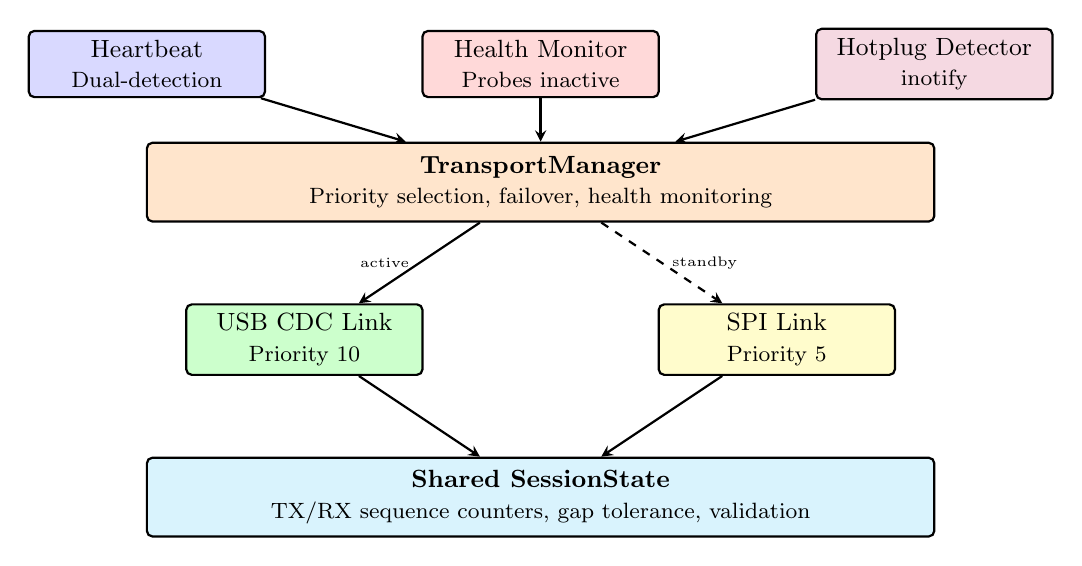
\begin{tikzpicture}[
    font=\small,
    node distance=0.5cm,
    box/.style={draw, thick, rectangle, minimum width=4cm, minimum height=1cm, align=center, rounded corners=2pt},
    smallbox/.style={draw, thick, rectangle, minimum width=3cm, minimum height=0.8cm, align=center, rounded corners=2pt},
    arrow/.style={->, thick, >=stealth},
    dasharrow/.style={->, thick, >=stealth, dashed}
]
    % TransportManager
    \node[box, fill=orange!20, minimum width=10cm] (tm) at (0,0) {\textbf{TransportManager}\\{\footnotesize Priority selection, failover, health monitoring}};

    % Active indicator
    \node[smallbox, fill=green!20] (usb) at (-3,-2) {USB CDC Link\\{\footnotesize Priority 10}};
    \node[smallbox, fill=yellow!20] (spi) at (3,-2) {SPI Link\\{\footnotesize Priority 5}};

    % Subsystems
    \node[smallbox, fill=blue!15] (hb) at (-5,1.5) {Heartbeat\\{\footnotesize Dual-detection}};
    \node[smallbox, fill=red!15] (hm) at (0,1.5) {Health Monitor\\{\footnotesize Probes inactive}};
    \node[smallbox, fill=purple!15] (hp) at (5,1.5) {Hotplug Detector\\{\footnotesize inotify}};

    % Session State
    \node[box, fill=cyan!15, minimum width=10cm] (ss) at (0,-4) {\textbf{Shared SessionState}\\{\footnotesize TX/RX sequence counters, gap tolerance, validation}};

    % Arrows
    \draw[arrow] (tm) -- node[left, font=\tiny] {active} (usb);
    \draw[dasharrow] (tm) -- node[right, font=\tiny] {standby} (spi);
    \draw[arrow] (hb) -- (tm);
    \draw[arrow] (hm) -- (tm);
    \draw[arrow] (hp) -- (tm);
    \draw[arrow] (usb) -- (ss);
    \draw[arrow] (spi) -- (ss);
\end{tikzpicture}%
}

\vspace{0.3cm}

\noindent\colorbox{keyinsightcolor}{\parbox{\dimexpr\linewidth-2\fboxsep}{%
\textbf{Key Insight:} The gateway sends on exactly one transport at a time. It never sends the same command on both USB and SPI simultaneously. The RX72N firmware listens on both channels but the gateway's single-active-transport design means only one will have data at any given moment (except during brief failover transitions).
}}

\subsection{Priority System}

Each transport is registered with a numeric priority. Higher values indicate preferred transports:

\begin{table}[H]
\centering
\caption{Transport Priority Configuration}
\label{tab:failover-priorities}
\begin{tabular}{l c l l}
\toprule
\textbf{Transport} & \textbf{Priority} & \textbf{Role} & \textbf{Rationale} \\
\midrule
USB CDC & 10 & Primary   & Lower latency, hardware CRC, no HARQ overhead \\
SPI     & 5  & Backup    & Always available, full HARQ protection \\
\bottomrule
\end{tabular}
\end{table}

\textbf{Priority rules:}
\begin{enumerate}[leftmargin=1.5em,topsep=4pt,itemsep=2pt]
    \item At startup, the transport with the highest priority that is healthy becomes active.
    \item If the active transport fails, switch to the highest-priority healthy alternative.
    \item If a higher-priority transport recovers, switch back to it (after damping period).
    \item Priority values are constants defined at compile time, not configurable at runtime.
\end{enumerate}

\subsection{Dual-Detection Heartbeat}

The heartbeat system uses two independent mechanisms to detect transport failures. This provides both fast failure detection (implicit) and explicit liveness checking (PING/PONG).

\subsubsection{Implicit Heartbeat (200\,ms Timeout)}

Any valid frame received on a transport resets that transport's implicit heartbeat timer. If no frame arrives within 200\,ms, the transport is considered unhealthy.

\begin{itemize}[leftmargin=1.5em,topsep=4pt,itemsep=2pt]
    \item \textbf{Timer reset:} Every valid frame (COMMAND, RESPONSE, TELEMETRY, PONG, ACK) resets the timer.
    \item \textbf{Timeout:} 200\,ms with no frames $\rightarrow$ mark transport as \texttt{degraded}.
    \item \textbf{No extra traffic:} Piggybacked on existing data flow. In normal operation at 100\,Hz (10\,ms between frames), the implicit timer never fires.
    \item \textbf{Fast detection:} If the USB cable is unplugged mid-stream, detection occurs within 200\,ms.
\end{itemize}

\subsubsection{Explicit Heartbeat (1\,s PING/PONG)}

When the link is idle (no data frames for 1\,second), the gateway sends a PING frame and expects a PONG response within 200\,ms.

\begin{itemize}[leftmargin=1.5em,topsep=4pt,itemsep=2pt]
    \item \textbf{PING interval:} Sent after 1\,second of idle (no other frames sent or received).
    \item \textbf{PONG timeout:} 200\,ms. If no PONG arrives, the transport is marked unhealthy.
    \item \textbf{Purpose:} Detects silent failures where the physical connection exists but the remote device is unresponsive (e.g., firmware crash, watchdog reset).
    \item \textbf{Frame types:} PING = \texttt{0x00}, PONG = \texttt{0x01} (see frame type table in Section~\ref{sec:communication-stack}).
\end{itemize}

\textbf{Why two mechanisms?}
\begin{itemize}[leftmargin=1.5em,topsep=4pt,itemsep=2pt]
    \item \textbf{Implicit} catches failures during active communication (fast: 200\,ms).
    \item \textbf{Explicit} catches failures during idle periods (slower: 1\,s + 200\,ms).
    \item Neither generates unnecessary traffic alone. Combined, they cover all scenarios.
\end{itemize}

\subsection{Health Monitoring}

The \texttt{HealthMonitor} (\texttt{internal/manager/health\_monitor.go}) runs a background goroutine that periodically probes \textbf{inactive} transports to detect when they recover. It does not interfere with the active transport.

\subsubsection{Health Thresholds}

A transport is considered unhealthy if \textbf{any} of the following conditions are met:

\begin{table}[H]
\centering
\caption{Health Monitoring Thresholds}
\label{tab:health-thresholds}
\begin{tabular}{l l l}
\toprule
\textbf{Metric} & \textbf{Threshold} & \textbf{Detection Method} \\
\midrule
Consecutive failures  & $\geq 3$         & Send or receive returns error 3 times in a row \\
Average latency       & $> 200$\,ms      & Exponential moving average of round-trip times \\
Packet loss rate      & $> 10\%$         & Sliding window over recent operations \\
\bottomrule
\end{tabular}
\end{table}

\subsubsection{Probing Inactive Transports}

The health monitor checks inactive transports every 5 seconds (configurable via \texttt{HealthCheckInterval}):

\begin{enumerate}[leftmargin=1.5em,topsep=4pt,itemsep=2pt]
    \item Select all transports that are \textbf{not} the currently active transport.
    \item For each inactive transport, send a PING and wait for PONG.
    \item If PONG received within timeout: mark transport as healthy, record recovery timestamp.
    \item If probe fails: keep transport marked as unhealthy.
    \item If a recovered transport has \textbf{higher priority} than the current active transport, trigger failover (subject to damping window).
\end{enumerate}

\subsection{Failover State Machine}

The \texttt{TransportManager} operates as a state machine with the following states:

\begin{table}[H]
\centering
\caption{Transport Manager States}
\label{tab:tm-states}
\begin{tabular}{l l p{7cm}}
\toprule
\textbf{State} & \textbf{Constant} & \textbf{Description} \\
\midrule
Active USB   & \texttt{StateActiveUSB}   & USB CDC is the active transport, SPI is standby \\
Active SPI   & \texttt{StateActiveSPI}   & SPI is the active transport, USB is unavailable or unhealthy \\
Degraded     & \texttt{StateDegraded}    & Active transport is unhealthy but no better alternative exists \\
Failed       & \texttt{StateFailed}      & No healthy transports available \\
\bottomrule
\end{tabular}
\end{table}

\subsubsection{State Transitions}

\vspace{0.3cm}

\noindent\makebox[\textwidth]{%
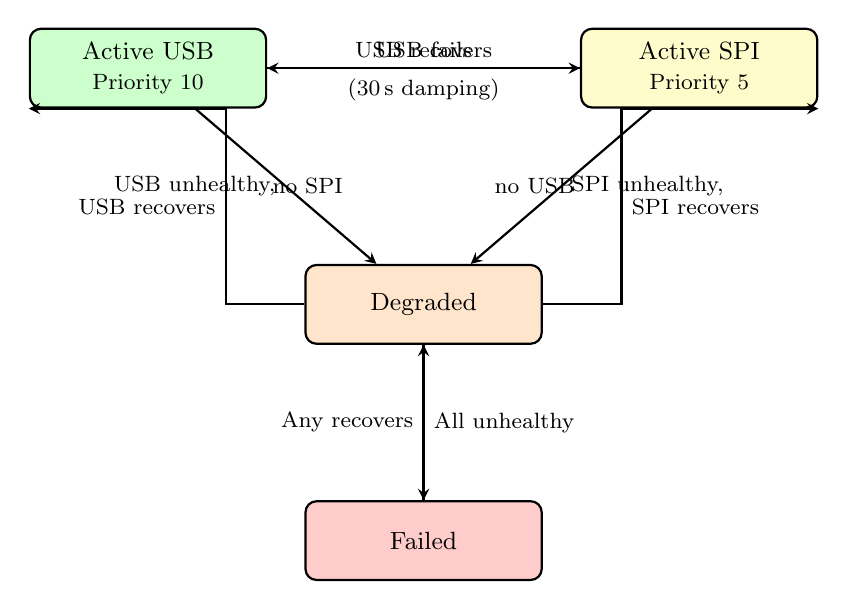
\begin{tikzpicture}[
    font=\small,
    node distance=2.5cm,
    state/.style={draw, thick, rectangle, minimum width=3cm, minimum height=1cm, align=center, rounded corners=4pt},
    arrow/.style={->, thick, >=stealth}
]
    \node[state, fill=green!20] (usb) at (0,0) {Active USB\\{\footnotesize Priority 10}};
    \node[state, fill=yellow!20] (spi) at (7,0) {Active SPI\\{\footnotesize Priority 5}};
    \node[state, fill=orange!20] (deg) at (3.5,-3) {Degraded};
    \node[state, fill=red!20] (fail) at (3.5,-6) {Failed};

    \draw[arrow] (usb) -- node[above, font=\footnotesize] {USB fails} (spi);
    \draw[arrow] (spi) -- node[above, font=\footnotesize] {USB recovers} node[below, font=\footnotesize] {(30\,s damping)} (usb);
    \draw[arrow] (usb) -- node[left, font=\footnotesize] {USB unhealthy,} node[right, font=\footnotesize, xshift=-0.3cm] {no SPI} (deg);
    \draw[arrow] (spi) -- node[right, font=\footnotesize] {SPI unhealthy,} node[left, font=\footnotesize, xshift=0.3cm] {no USB} (deg);
    \draw[arrow] (deg) -- node[right, font=\footnotesize] {All unhealthy} (fail);
    \draw[arrow] (fail) -- node[left, font=\footnotesize] {Any recovers} (deg);
    \draw[arrow] (deg.west) -- ++(-1,0) |- node[left, font=\footnotesize, near start] {USB recovers} (usb.south west);
    \draw[arrow] (deg.east) -- ++(1,0) |- node[right, font=\footnotesize, near start] {SPI recovers} (spi.south east);
\end{tikzpicture}%
}

\subsection{Smart Drain}

When switching away from a transport, the gateway uses ``smart drain'' to handle in-flight frames gracefully:

\begin{itemize}[leftmargin=1.5em,topsep=4pt,itemsep=2pt]
    \item \textbf{Hard failure (IO error, disconnect):} Skip drain entirely. Switch immediately. In-flight frames are lost but speed is critical --- the motor control loop cannot afford a 500\,ms pause.
    \item \textbf{Graceful degradation (high latency, packet loss):} Wait up to 500\,ms for in-flight frames to complete before switching. This avoids losing frames that are nearly delivered.
\end{itemize}

\textbf{Failover timing with smart drain:}

\begin{table}[H]
\centering
\caption{Failover Timing by Failure Type}
\label{tab:failover-timing}
\begin{tabular}{l l l}
\toprule
\textbf{Failure Type} & \textbf{Detection} & \textbf{Total Failover Time} \\
\midrule
USB cable unplugged     & $\sim$200\,ms (implicit timeout) & $< 300$\,ms (no drain) \\
USB device hang         & $\sim$1.2\,s (PING timeout)      & $< 1.5$\,s (no drain) \\
High latency            & $\sim$200\,ms (threshold)        & $< 700$\,ms (500\,ms drain) \\
RX72N firmware crash    & $\sim$1.2\,s (PING timeout)      & $< 1.5$\,s (no drain) \\
\bottomrule
\end{tabular}
\end{table}

\noindent\colorbox{importantcolor}{\parbox{\dimexpr\linewidth-2\fboxsep}{%
\textbf{Important:} The worst-case failover time (1.5\,s) is well within the RX72N's 500\,ms communication watchdog on the \emph{active} transport, but frames from the \emph{standby} transport would arrive before the watchdog fires. The 500\,ms watchdog applies to total communication silence, not to any individual transport.
}}

\subsection{Shared SessionState (Preventing the Handoff Problem)}
\label{subsec:shared-session}

The ``Handoff Problem'' occurs when two transports maintain separate sequence counters:

\begin{enumerate}[leftmargin=1.5em,topsep=4pt,itemsep=2pt]
    \item Gateway sends frames 1--100 over USB (USB sequence = 100, SPI sequence = 0).
    \item USB fails. Gateway switches to SPI.
    \item If SPI has its own counter starting at 0, the RX72N sees sequence ``jump'' from 100 to 0.
    \item The RX72N rejects frame 0 as a duplicate (already seen sequence 0 from USB earlier).
    \item \textbf{Result:} Total communication failure after failover.
\end{enumerate}

\textbf{Solution:} Both transports share a single \texttt{SessionState} object that owns the TX and RX sequence counters:

\begin{lstlisting}[language=Go, caption={Shared SessionState (manager/session.go)}]
type SessionState struct {
    mu         sync.Mutex
    txSequence uint16  // Shared TX counter (both USB and SPI)
    rxSequence uint16  // Shared RX counter (both USB and SPI)
    gapMax     uint16  // Maximum acceptable sequence gap (default: 10)
}

func (s *SessionState) NextTxSequence() uint16 {
    s.mu.Lock()
    defer s.mu.Unlock()
    seq := s.txSequence
    s.txSequence++
    return seq
}
\end{lstlisting}

\textbf{After failover:} Gateway sends frames 1--100 over USB, then frame 101 over SPI. The RX72N sees a continuous sequence regardless of which physical transport delivered it.

\subsubsection{Gap Tolerance}

The shared \texttt{SessionState} accepts sequence gaps of up to 10 frames (\texttt{gapMax = 10}). This handles:

\begin{itemize}[leftmargin=1.5em,topsep=4pt,itemsep=2pt]
    \item \textbf{Rare USB packet loss:} A frame lost during transmission creates a gap of 1. The next frame (sequence $N+1$) is accepted despite the missing $N$.
    \item \textbf{Failover transitions:} During the switch, 1--3 frames may be in-flight on the old transport and never delivered. The new transport picks up at the next sequence number.
    \item \textbf{Duplicate rejection:} Frames with sequences $\leq$ the last accepted sequence are rejected as duplicates (prevents replay).
\end{itemize}

\subsection{USB Hot-Plug Detection}
\label{subsec:hotplug}

The gateway uses Linux \texttt{inotify} to detect USB device attach/detach events in real time, without polling:

\begin{itemize}[leftmargin=1.5em,topsep=4pt,itemsep=2pt]
    \item \textbf{Watch path:} \texttt{/sys/bus/usb/devices} (Linux sysfs)
    \item \textbf{Events:} \texttt{IN\_CREATE} (device attached), \texttt{IN\_DELETE} (device removed)
    \item \textbf{Latency:} Near-instant ($< 50$\,ms from physical plug/unplug to software notification)
    \item \textbf{Filter:} Only reacts to changes matching the RX72N's USB VID/PID (\texttt{045B:0261}, Renesas RX)
\end{itemize}

\textbf{Hot-plug flow:}
\begin{enumerate}[leftmargin=1.5em,topsep=4pt,itemsep=2pt]
    \item USB cable plugged in $\rightarrow$ inotify fires \texttt{IN\_CREATE}.
    \item Hotplug detector opens \texttt{/dev/ttyACM0}, creates USB transport and CDC link.
    \item Registers new transport with \texttt{TransportManager} (priority 10).
    \item If USB has higher priority than current transport $\rightarrow$ switch to USB.
    \item USB cable unplugged $\rightarrow$ inotify fires \texttt{IN\_DELETE}.
    \item Hotplug detector notifies \texttt{TransportManager} $\rightarrow$ immediate failover to SPI.
\end{enumerate}

\subsection{Failback Damping (30-Second Cooldown)}
\label{subsec:failback-damping}

When a previously failed transport recovers, the gateway does \textbf{not} switch back immediately. A 30-second damping window prevents rapid oscillation (``flapping'') between transports:

\begin{itemize}[leftmargin=1.5em,topsep=4pt,itemsep=2pt]
    \item \textbf{Scenario:} USB fails, gateway switches to SPI. USB recovers 2 seconds later.
    \item \textbf{Without damping:} Gateway immediately switches back to USB. If USB is intermittent, it fails again 1 second later. Gateway switches to SPI again. This ``flapping'' disrupts communication.
    \item \textbf{With damping:} Gateway records the USB recovery timestamp. Waits 30 seconds. Only if USB has been continuously healthy for 30 seconds does the gateway switch back.
\end{itemize}

\textbf{Damping parameters:}

\begin{table}[H]
\centering
\caption{Failback Damping Parameters}
\label{tab:damping-params}
\begin{tabular}{l l l}
\toprule
\textbf{Parameter} & \textbf{Value} & \textbf{Description} \\
\midrule
Damping window     & 30\,s       & Minimum healthy duration before failback \\
Health check rate   & 5\,s        & How often inactive transports are probed \\
Recovery condition  & 6 consecutive healthy probes & 6 $\times$ 5\,s = 30\,s of health \\
\bottomrule
\end{tabular}
\end{table}

\subsection{Reset Handshake (Gateway Restart Recovery)}
\label{subsec:reset-handshake}

When the gateway restarts (process crash, reboot, update), the RX72N may still be running with sequence counters at, say, 5000. The restarted gateway's counters start at 0. Without synchronization, the RX72N would reject all frames as out-of-sequence.

\textbf{Three-way reset handshake:}
\begin{enumerate}[leftmargin=1.5em,topsep=4pt,itemsep=2pt]
    \item \textbf{Gateway $\rightarrow$ RX72N:} Send \texttt{RESET} frame (type \texttt{0xFF}).
    \item \textbf{RX72N $\rightarrow$ Gateway:} Respond with \texttt{RESET\_ACK} frame (type \texttt{0xFE}). RX72N resets its TX/RX counters to 0.
    \item \textbf{Gateway:} Receives \texttt{RESET\_ACK}, resets its own SessionState counters to 0.
    \item Both sides are now synchronized at sequence 0. Normal communication resumes.
\end{enumerate}

\textbf{Timeout:} If no \texttt{RESET\_ACK} is received within 500\,ms, the gateway retries the \texttt{RESET} frame (up to 3 times). If all retries fail, the gateway assumes the RX72N is unreachable and enters the \texttt{StateFailed} state.

\noindent\colorbox{importantcolor}{\parbox{\dimexpr\linewidth-2\fboxsep}{%
\textbf{Important:} The reset handshake prevents a ``restart deadlock'' where the gateway cannot communicate because sequences are mismatched, and the RX72N cannot be told to reset because it rejects the out-of-sequence reset frame. The RESET frame type is handled specially by the RX72N --- it is always accepted regardless of sequence number.
}}

\subsection{Firmware Side: Passive Listener}

The RX72N firmware does not participate in transport selection. It is a \textbf{passive listener} that:

\begin{enumerate}[leftmargin=1.5em,topsep=4pt,itemsep=2pt]
    \item Listens on both USB CDC and SPI simultaneously.
    \item Accepts valid frames from either channel (validated by CRC-32 and sequence number).
    \item Does not know or care which transport the gateway considers ``active.''
    \item Routes all received commands through the same callback (\texttt{internal\_frame\_callback}).
    \item Sends telemetry on whichever channel last received a command (implicit response routing).
\end{enumerate}

The \texttt{rx\_comm\_manager\_poll()} function (\texttt{rx\_comm\_manager.c:1317}) polls both channels sequentially every 10\,ms (100\,Hz):

\begin{lstlisting}[language=C, caption={RX72N Dual-Channel Polling}]
rx_err_t rx_comm_manager_poll(rx_comm_manager_t* mgr) {
    /* Poll USB first */
    rx_err_t usb_err = internal_poll_usb(mgr);
    /* Poll SPI second */
    rx_err_t spi_err = internal_poll_spi(mgr);
    /* Process event queue */
    internal_process_event_queue(mgr);
    /* Check heartbeat timers */
    internal_check_heartbeat(mgr);
    return received ? k_rx_ok : k_rx_err_timeout;
}
\end{lstlisting}

\subsection{Timing Summary}

\begin{table}[H]
\centering
\caption{Transport Failover Timing Summary}
\label{tab:failover-timing-summary}
\begin{tabular}{l l}
\toprule
\textbf{Event} & \textbf{Timing} \\
\midrule
Implicit heartbeat timeout      & 200\,ms \\
Explicit PING interval          & 1\,s idle \\
PING/PONG timeout               & 200\,ms \\
Health check interval           & 5\,s \\
Smart drain (graceful)          & up to 500\,ms \\
Smart drain (hard failure)      & 0\,ms (immediate) \\
Failback damping window         & 30\,s \\
Reset handshake timeout         & 500\,ms per attempt, 3 retries \\
RX72N comm watchdog             & 500\,ms \\
USB hot-plug detection           & $< 50$\,ms \\
Worst-case failover (cable pull) & $< 300$\,ms \\
Worst-case failover (silent)     & $< 1.5$\,s \\
\bottomrule
\end{tabular}
\end{table}

\subsection{Cross-References}

\begin{itemize}[leftmargin=1.5em,topsep=4pt,itemsep=2pt]
    \item \textbf{Section~\ref{sec:communication-stack}}: Protocol stack, HARQ details, frame format
    \item \textbf{Section~\ref{sec:dual-channel-arbitration}}: How the RX72N handles simultaneous data on both channels
    \item \textbf{Section~\ref{sec:gateway-architecture}}: Gateway service architecture and directory structure
    \item \textbf{Section~\ref{sec:usb_cdc_protocol}}: USB CDC transport details
    \item \texttt{star-gateway/internal/manager/manager.go}: TransportManager implementation
    \item \texttt{star-gateway/internal/manager/heartbeat.go}: Dual-detection heartbeat
    \item \texttt{star-gateway/internal/manager/health\_monitor.go}: Health probing for inactive transports
    \item \texttt{star-gateway/internal/manager/hotplug\_detector.go}: USB inotify-based hot-plug detection
    \item \texttt{star-gateway/internal/manager/session.go}: Shared SessionState
\end{itemize}


% Section 14: Dual-Channel Arbitration
% == == == == == == == == == == == == == == == == == == == == == == == == == ==
    == == == == == == == == == == == ==
    = % DUAL - CHANNEL ARBITRATION % == == == == == == == == == == == == == ==
      == == == == == == == == == == == == == == == == == == == == == == == ==
    =

\newpage
\section{Dual - Channel Arbitration on the RX72N
}
\label{sec : dual - channel - arbitration}

This section documents how the RX72N firmware handles the case where data
    arrives on both USB CDC and SPI simultaneously,
    what ordering guarantees exist,
    and why the architecture prevents conflicts
            .

\subsection{The Question}

        The RX72N listens on both USB CDC and SPI at all times
            .What happens if frames arrive on both channels at the same time,
    potentially carrying different data ?

\subsection{Gateway Guarantee:
Single Active Transport
}

Under normal operation, this scenario \textbf{cannot occur} because the gateway's \texttt{TransportManager} maintains exactly one active transport:

\begin{lstlisting}[language = Go,
                        caption = {Gateway sends on ONE transport only(
                            manager.go)}] func(tm *TransportManager)
                            Send(ctx context.Context, data[] byte, ...) error {
  tm.mu.RLock() active : = tm.activeTransport // Only ONE transport
                               activeName
      : = tm.activeTransportName tm.mu.RUnlock()

              if active ==
          nil{return errors.New("no active transport available")}

          err : = active.Send(ctx, data, p...) // Send on THAT one only
                                               // ...
}
\end{lstlisting}

    The gateway \textbf{never} sends the same command on both USB and
        SPI simultaneously.It selects
        one(USB preferred, priority 10) and
    sends exclusively on that.

\subsection{When Overlap Can Occur}

        Despite the single
        - active - transport guarantee,
    brief overlap is possible during failover transitions :

\begin{enumerate}[leftmargin = 1.5em, topsep = 4pt, itemsep = 2pt]
    \item \textbf{In - flight frame during failover :
   } Frame $N$ was transmitted on USB and is still being processed by the USB
    hardware when the gateway detects a failure and switches to SPI.Frame $N
        + 1 $ is sent on SPI.The RX72N receives both frames in the same 10\,
    ms poll cycle.
    \item \textbf{Telemetry crossing :} The RX72N sends telemetry on
    USB(because the last command came from USB),
    while the gateway has already switched to SPI and sends a new command on SPI
        .The firmware receives the SPI command while USB telemetry is outgoing.
\end{enumerate}

\subsection{Sequential Polling : USB First, Then SPI}

The \texttt{rx\_comm\_manager\_poll()} function processes channels \textbf{sequentially},
    not in parallel.There is no race condition because the entire function runs
            in a single
            thread(\texttt{comm\_task}, ThreadX Priority 5, 100\, Hz)
    :

\begin{lstlisting}[language = C, caption = {Sequential channel polling(
                                      rx\_comm\_manager\_poll)}] rx_err_t
          rx_comm_manager_poll(rx_comm_manager_t * mgr) {
  bool received = false;

  /* Step 1: Poll USB channel */
  rx_err_t usb_err = internal_poll_usb(mgr);
  if (usb_err == k_rx_ok) {
    received = true; // USB frame processed
 }

  /* Step 2: Poll SPI channel */
  rx_err_t spi_err = internal_poll_spi(mgr);
  if (spi_err == k_rx_ok) {
    received = true; // SPI frame processed
 }

  /* Step 3: Process event queue */
  internal_process_event_queue(mgr);

  /* Step 4: Check heartbeat timers */
  internal_check_heartbeat(mgr);

  return received ? k_rx_ok : k_rx_err_timeout;
}
\end{lstlisting}

\textbf{Ordering guarantee :} Within any single poll cycle,
    USB is always processed before SPI.This is deterministic and repeatable.

\subsection{Frame Processing Pipeline}

        Both \texttt{
            internal\_poll\_usb()} and \texttt{internal\_poll\_spi()} follow the
            same pipeline :

\vspace {
  0.3cm
}

\noindent\makebox[\textwidth] {
  %
\begin{tikzpicture}[font =\small, node distance=0.3cm,
                     box/.style={draw, thick, rectangle, minimum width = 4cm,
                                    minimum height = 0.8cm, align = center,
                                    rounded corners = 2pt},
                     arrow/.style={->, thick, >= stealth}] %
      USB path
    \node[box, fill=blue!15](usb_recv)
          at(0, 0){USB : rx\_usb\_comm\_receive()};
  \node[box, fill=yellow!15, below=of usb_recv](usb_handle){
      internal\_handle\_frame(USB)};
  \node[box, fill=green!15, below=of usb_handle](usb_cb){
      internal\_frame\_callback()};
  \node[box, fill=orange!15, below=of usb_cb](usb_cmd){
      shared\_data\_set\_motor\_command()};

  % SPI path
    \node[box, fill=red!15](spi_recv)
          at(7, 0){SPI : rx\_spi\_link\_receive()};
  \node[box, fill=yellow!15, below=of spi_recv](spi_handle){
      internal\_handle\_frame(SPI)};
  \node[box, fill=green!15, below=of spi_handle](spi_cb){
      internal\_frame\_callback()};
  \node[box, fill=orange!15, below=of spi_cb](spi_cmd){
      shared\_data\_set\_motor\_command()};

  % Arrows
    \draw[arrow](usb_recv)--(usb_handle);
  \draw[arrow](usb_handle)--(usb_cb);
  \draw[arrow](usb_cb)--(usb_cmd);
  \draw[arrow](spi_recv)--(spi_handle);
  \draw[arrow](spi_handle)--(spi_cb);
  \draw[arrow](spi_cb)--(spi_cmd);

  % Time arrow
    \draw[->, very thick, gray](-2.5, 0.5)--(
        -2.5, -4)node[below, font =\footnotesize]{Time};

  % Labels
    \node[above, font =\footnotesize\bfseries] at(usb_recv.north){
        Processed First};
  \node[above, font =\footnotesize\bfseries] at(spi_recv.north){
      Processed Second};

  % Overwrite indicator
    \draw[->, thick, red, dashed](
        spi_cmd.west)-- node[below, font =\footnotesize\color{red}]{
        Overwrites}(usb_cmd.east);
  \end{tikzpicture} %
}

\vspace { 0.3cm}

\subsection{Last Writer Wins}

Both frames call \texttt{shared\_data\_set\_motor\_command(\& cmd)},
    which is mutex -
        protected.Since the two calls execute sequentially(not concurrently),
    the second call \textbf{overwrites} the first :

\begin{enumerate}[leftmargin = 1.5em, topsep = 4pt, itemsep = 2pt]
    \item USB frame arrives $\rightarrow$ \texttt{
        shared\_data\_set\_motor\_command()} writes motor
    velocities from USB frame.
    \item SPI frame arrives $\rightarrow$ \texttt {
  shared\_data\_set\_motor\_command()
}
\textbf{overwrites} with motor velocities from SPI frame.
    \item Motor task wakes up $\rightarrow$ reads the \textbf{SPI frame's data} (the last one written).
\end{enumerate}

\textbf{The SPI command wins because it is polled second.} The USB command is effectively superseded.

\subsection{Why This Is Correct During Failover}

During a failover, the overlap works \textbf{correctly} because the gateway uses shared \texttt{SessionState} sequence numbers:

\begin{enumerate}[leftmargin=1.5em,topsep=4pt,itemsep=2pt]
    \item The gateway increments the sequence number for each \texttt{Send()} call (shared counter).
    \item Frame $N$ goes out on USB (the old transport).
    \item Frame $N+1$ goes out on SPI (the new transport).
    \item The RX72N processes USB ($N$) first, then SPI ($N+1$) second.
    \item The motor task gets frame $N+1$, which is the \textbf{newer} command.
    \item This is the correct behavior --- the motor should execute the most recent command.
\end{enumerate}

\noindent\colorbox{keyinsightcolor} {
  \parbox{\dimexpr\linewidth - 2\fboxsep} {
    %
\textbf{Key Insight :
   } The ``last writer wins'' semantics combined with sequential
             polling(USB before SPI) and
        monotonically increasing sequence numbers guarantee that the motor task
            always receives the most recent command,
        even during transport failover.
 }
}

\subsection{Sequence Validation}

The shared \texttt{
    rx\_session} module on the RX72N validates every received sequence number :

\begin{itemize}[leftmargin = 1.5em, topsep = 4pt, itemsep = 2pt]
    \item \textbf{Duplicate detection :} If the same sequence number is received
    twice (e.g., frame retransmitted on both channels),
    the second copy is rejected by \texttt{rx\_session\_validate\_rx()}.
    \item \textbf{Gap tolerance :} Sequence gaps of up to 10 frames are accepted
    (see Section ~\ref{subsec : shared - session}).
    This handles frames lost during failover.
    \item \textbf{Wraparound:
}
16 - bit sequence numbers wrap from 65535 to 0. The validation logic
         handles this correctly.
\end{itemize}

\subsection{Channel Parameter(Currently Unused)}

    The \texttt{internal\_handle\_command\_frame()} function receives a \texttt{
        channel} parameter indicating whether the frame arrived on USB or
    SPI :

\begin{lstlisting}[language = C,
                    caption = {Channel parameter in command handler(
                        internal\_handle\_velocity\_request)}] static void
    internal_handle_command_frame(rx_comm_channel_t channel,
                                  const rx_frame_t *frame) {
  (void)channel; // Currently unused
                 // ... decode protobuf, update shared_data ...
}
\end{lstlisting}

The channel parameter is currently cast to \texttt{void} (unused). A future enhancement could use it to:
\begin{itemize}[leftmargin=1.5em,topsep=4pt,itemsep=2pt]
    \item Route response/telemetry back on the same channel that sent the command.
    \item Log which channel is actively receiving commands for diagnostics.
    \item Implement channel-specific command filtering (e.g., only accept emergency stop from USB).
\end{itemize}

\subsection{Communication Watchdog Interaction}

The 500\,
    ms communication watchdog(\texttt{shared\_data\_update\_last\_comm\_tick()})
        is updated on \textbf{every valid frame from either channel} :

\begin{lstlisting}[language = C, caption = {Watchdog update on any frame(
                                      internal\_update\_watchdog)}] static void
            internal_frame_callback(rx_comm_channel_t channel,
                                    const rx_frame_t *frame, void *ctx) {
  (void)ctx;
  if (frame == nullptr) {
    return;
 }

  /* Update watchdog on ANY valid frame from ANY channel */
  shared_data_update_last_comm_tick();

  switch (frame->header.type) {
  case k_frame_type_command:
    internal_handle_command_frame(channel, frame);
    break;
    // ...
 }
}
\end{lstlisting}

This means :
\begin{itemize}[leftmargin = 1.5em, topsep = 4pt, itemsep = 2pt]
    \item During failover,
    if USB stops sending but SPI starts,
    the watchdog is still satisfied.
    \item The 500\,
    ms timer only triggers emergency stop if \textbf{both} channels are completely silent
        .
    \item A single valid frame on either channel resets
            the watchdog and prevents emergency stop.
\end{itemize}

\subsection{Summary:
  Dual - Channel Behavior Matrix
}

\begin{table}[H]
\centering
\caption {RX72N Behavior for Dual-Channel Scenarios
}
\label {
tab:
  dual - channel - matrix
}
\begin{tabular} { l l l}
\toprule
\textbf{Scenario} & \textbf{What Happens} & \textbf{Result} \\
\midrule
Normal operation    & Gateway sends on ONE channel only          & Single frame per cycle \\
Failover overlap    & Both channels have data                   & USB processed first, SPI overwrites \\
                    &                                           & (newer command = correct) \\
Duplicate frame     & Same sequence on both channels             & Sequence validation rejects second \\
Different senders   & Cannot happen (single gateway)            & Architecture prevents this \\
All channels silent & No frames for 500\,ms                     & Emergency stop triggered \\
One channel fails   & Other channel still delivers frames       & Watchdog still satisfied \\
\bottomrule
\end{tabular}
\end{table}

\subsection{Cross - References}

\begin{itemize}[leftmargin = 1.5em, topsep = 4pt, itemsep = 2pt]
    \item \textbf{Section ~\ref{sec : communication - stack}} : Protocol stack,
                                                                 frame format,
                                                                 CRC validation
    \item \textbf{Section ~\ref{sec : transport - failover}}
    : Transport failover,
      health monitoring,
      shared SessionState
    \item \texttt{e2 - studio - star - rx72n -
                   firmware / libs / rx\_comm\_manager / src /
                       rx\_comm\_manager.c}
    : Dual -
      channel polling implementation
    \item \texttt{e2 - studio - star - rx72n -
                   firmware / src / tasks / comm\_task.c} : Frame callback,
      command dispatch,
      watchdog update
    \item \texttt{star - gateway / internal / manager / manager.go}
    : Single -
      active - transport guarantee
\end{itemize}


% Section 9: USB CDC Debug Protocol
\section{USB CDC Protocol}
\label{sec:usb_cdc_protocol}

\subsection{Overview}

The RX72N firmware implements a USB CDC-ACM (Communications Device Class - Abstract Control Model) composite device with three independent virtual serial ports. This enables simultaneous binary protocol communication, ASCII debugging, and log streaming over a single USB connection.

\subsubsection{Port Assignment}

\begin{table}[h]
\centering
\begin{tabular}{|c|l|l|c|c|p{4cm}|}
\hline
\textbf{Port} & \textbf{Purpose} & \textbf{Linux Device} & \textbf{RX (B)} & \textbf{TX (B)} & \textbf{Usage} \\
\hline
0 & Protocol & /dev/ttyACM0 & 1024 & 1024 & nanopb frames, motor commands \\
1 & Decoded & /dev/ttyACM1 & 256 & 512 & ASCII frame dumps, debugging \\
2 & Log & /dev/ttyACM2 & 256 & 1024 & System logging, diagnostics \\
\hline
\end{tabular}
\caption{USB CDC Port Configuration}
\label{tab:usb_cdc_ports}
\end{table}

\subsubsection{Hardware Configuration}

\begin{itemize}
\item \textbf{USB Speed}: Full-Speed (12 Mbps)
\item \textbf{Max Packet Size}: 64 bytes (bulk endpoints)
\item \textbf{Pipes Used}: 9 pipes total (1 control + 3 CDC × (1 interrupt + 2 bulk))
\item \textbf{Pins}: USB\_DP (PA4), USB\_DM (PA5), USB\_VBUS (PA6)
\item \textbf{Clock}: 48 MHz USB clock from PLL
\end{itemize}

\subsection{USB Descriptor Hierarchy}

\subsubsection{Device Descriptor}

\begin{lstlisting}[language=C,caption={USB Device Descriptor},label={lst:usb_device_desc}]
{
  .bLength = 18,
  .bDescriptorType = USB_DEVICE_DESCRIPTOR,
  .bcdUSB = 0x0200,              // USB 2.0
  .bDeviceClass = 0xEF,          // Miscellaneous (IAD)
  .bDeviceSubClass = 0x02,       // Common Class
  .bDeviceProtocol = 0x01,       // Interface Association
  .bMaxPacketSize0 = 64,
  .idVendor = 0x045B,            // Renesas
  .idProduct = 0x024F,           // RX72N CDC
  .bcdDevice = 0x0100,           // Device v1.0
  .iManufacturer = 1,            // "STAR Project"
  .iProduct = 2,                 // "RX72N CDC Composite"
  .iSerialNumber = 3,            // "RX72N-00001"
  .bNumConfigurations = 1
}
\end{lstlisting}

\subsubsection{Configuration Descriptor}

The configuration descriptor contains:
\begin{itemize}
\item 3 × Interface Association Descriptors (IAD) - Groups each CDC function
\item 3 × CDC Control Interface (Class 0x02, Subclass 0x02)
\item 3 × CDC Data Interface (Class 0x0A, Subclass 0x00)
\item 3 × Interrupt IN endpoints (control)
\item 6 × Bulk endpoints (3 IN + 3 OUT for data)
\end{itemize}

\subsubsection{Interface Association Descriptor (IAD)}

Each CDC port uses an IAD to group its control and data interfaces:

\begin{lstlisting}[language=C,caption={IAD for Port 0 (Protocol Port)},label={lst:usb_iad}]
{
  .bLength = 8,
  .bDescriptorType = 0x0B,       // IAD
  .bFirstInterface = 0,          // Control interface
  .bInterfaceCount = 2,          // Control + Data
  .bFunctionClass = 0x02,        // CDC
  .bFunctionSubClass = 0x02,     // ACM
  .bFunctionProtocol = 0x01,     // AT Commands
  .iFunction = 4                 // "Protocol Port"
}
\end{lstlisting}

\subsubsection{Endpoint Configuration}

\begin{table}[h]
\centering
\begin{tabular}{|c|l|c|c|c|c|}
\hline
\textbf{Port} & \textbf{Type} & \textbf{EP} & \textbf{Dir} & \textbf{Size} & \textbf{Interval} \\
\hline
0 & Interrupt & EP1 & IN & 16 & 10 ms \\
0 & Bulk OUT & EP2 & OUT & 64 & - \\
0 & Bulk IN & EP3 & IN & 64 & - \\
\hline
1 & Interrupt & EP4 & IN & 16 & 10 ms \\
1 & Bulk OUT & EP5 & OUT & 64 & - \\
1 & Bulk IN & EP6 & IN & 64 & - \\
\hline
2 & Interrupt & EP7 & IN & 16 & 10 ms \\
2 & Bulk OUT & EP8 & OUT & 64 & - \\
2 & Bulk IN & EP9 & IN & 64 & - \\
\hline
\end{tabular}
\caption{USB Endpoint Assignments}
\label{tab:usb_endpoints}
\end{table}

\subsection{USB State Machine}

\begin{figure}[h]
\centering
\begin{tikzpicture}[node distance=2cm, auto]
  \node[state] (detached) {Detached};
  \node[state, right of=detached] (attached) {Attached};
  \node[state, right of=attached] (powered) {Powered};
  \node[state, below of=powered] (default) {Default};
  \node[state, left of=default] (addressed) {Addressed};
  \node[state, left of=addressed] (configured) {Configured};
  \node[state, below of=configured] (suspended) {Suspended};

  \path[->]
    (detached) edge node {VBUS detect} (attached)
    (attached) edge node {auto} (powered)
    (powered) edge node {Bus Reset} (default)
    (default) edge node {SET\_ADDRESS} (addressed)
    (addressed) edge node {SET\_CONFIG} (configured)
    (configured) edge node {3ms idle} (suspended)
    (suspended) edge[bend right] node {Resume} (configured)
    (configured) edge[bend right=60] node[below] {VBUS lost} (detached)
    (default) edge[bend left=40] node {Bus Reset} (default);
\end{tikzpicture}
\caption{USB Device State Machine}
\label{fig:usb_state_machine}
\end{figure}

\textbf{Critical State}: Only in \texttt{Configured} state can \texttt{rx\_usb\_write/read} transfer data.

\subsection{CDC-ACM Class Requests}

The USB CDC driver handles these class-specific requests:

\begin{table}[h]
\centering
\begin{tabular}{|l|c|p{6cm}|}
\hline
\textbf{Request} & \textbf{Code} & \textbf{Description} \\
\hline
SET\_LINE\_CODING & 0x20 & Host configures baud rate, parity, stop bits \\
GET\_LINE\_CODING & 0x21 & Host queries current line coding \\
SET\_CONTROL\_LINE\_STATE & 0x22 & DTR/RTS control signals (ignored) \\
\hline
\end{tabular}
\caption{CDC-ACM Class Requests}
\label{tab:cdc_requests}
\end{table}

\textbf{Note}: Line coding settings (baud rate, parity, etc.) are informational only. USB CDC operates at USB Full-Speed (12 Mbps), not the configured baud rate.

\subsection{Bulk Transfer Protocol}

\subsubsection{Data Flow}

\paragraph{Bulk OUT (Host → Device)}

\begin{enumerate}
\item Host writes data to /dev/ttyACM*
\item USB driver sends bulk OUT packet (max 64 bytes)
\item RX72N receives packet → BRDY interrupt fires
\item ISR reads FIFO → copies to RX ring buffer
\item Application calls \texttt{rx\_usb\_read()} → retrieves data
\end{enumerate}

\paragraph{Bulk IN (Device → Host)}

\begin{enumerate}
\item Application calls \texttt{rx\_usb\_write()} → copies to TX ring buffer
\item ISR writes FIFO → sends bulk IN packet (max 64 bytes)
\item BEMP interrupt fires when packet sent
\item Host reads data from /dev/ttyACM*
\end{enumerate}

\subsubsection{FIFO Access Requirements (RX72N-Specific)}

\textbf{CRITICAL}: RX72N USB FIFO registers \textbf{must} be accessed as 16-bit words, NOT byte-by-byte.

\begin{lstlisting}[language=C,caption={Correct FIFO Read (16-bit access)},label={lst:fifo_read_correct}]
// CORRECT: Read CFIFO as 16-bit words
for (uint32_t i = 0; i < len; i += 2) {
  const uint16_t word = usb0()->cfifo;  // 16-bit read
  data[i] = (uint8_t)(word & 0xFF);     // Low byte
  if ((i + 1) < len) {
    data[i + 1] = (uint8_t)((word >> 8) & 0xFF);  // High byte
  }
}
\end{lstlisting}

\begin{lstlisting}[language=C,caption={Incorrect FIFO Read (causes data corruption)},label={lst:fifo_read_wrong}]
// WRONG: Byte-by-byte access causes corruption
for (uint32_t i = 0; i < len; i++) {
  data[i] = (uint8_t)(usb0()->cfifo & 0xFF);  // BAD!
}
\end{lstlisting}

\textbf{Impact}: Byte-by-byte access was the root cause of all bulk transfer failures before Phase 2 fixes.

\subsubsection{FIFO Clear Sequence}

Before writing to FIFO, the BCLR (Buffer Clear) sequence must be executed:

\begin{lstlisting}[language=C,caption={FIFO Clear Before Write},label={lst:fifo_clear}]
// Set BCLR bit (hardware clears FIFO)
usb0()->cfifoctr |= k_usb_fifoctr_bclr;

// Wait for BCLR to complete (hardware clears bit)
uint32_t timeout = 10000;
while ((usb0()->cfifoctr & k_usb_fifoctr_bclr) && timeout--) {
  __asm__ volatile("nop");
}

// Now safe to write data
for (uint32_t i = 0; i < len; i += 2) {
  // ... 16-bit write ...
}
\end{lstlisting}

\textbf{Impact}: Missing BCLR sequence caused first packet corruption with stale data.

\subsection{Debug Logging Over USB CDC Port 2}

\subsubsection{Architecture}

The logging system supports dual output to both UART and USB CDC Port 2:

\begin{itemize}
\item \textbf{UART (SCI12)}: Always works, independent of USB state
\item \textbf{USB CDC Port 2}: Enabled when \texttt{USB\_LOG\_MIRROR=1}
\item \textbf{Boot buffering}: 512B ring buffer for logs during USB enumeration (0-200ms)
\item \textbf{Thread safety}: ThreadX mutex for multi-task logging
\item \textbf{Non-blocking}: Drops logs on TX full, tracks statistics
\end{itemize}

\subsubsection{Boot Log Sequence}

\begin{figure}[h]
\centering
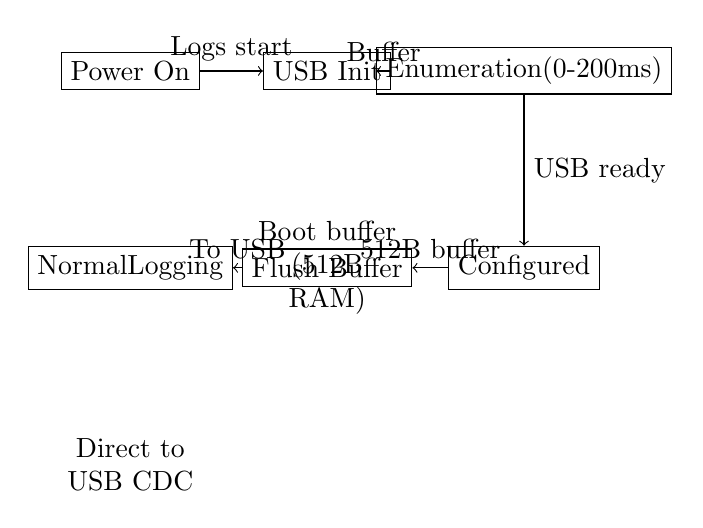
\begin{tikzpicture}[node distance=2.5cm, auto]
  \node[rectangle, draw] (power) {Power On};
  \node[rectangle, draw, right of=power] (usb_init) {USB Init};
  \node[rectangle, draw, right of=usb_init] (enum) {Enumeration\\(0-200ms)};
  \node[rectangle, draw, below of=enum] (configured) {Configured};
  \node[rectangle, draw, left of=configured] (flush) {Flush Buffer};
  \node[rectangle, draw, left of=flush] (normal) {Normal\\Logging};

  \draw[->] (power) -- node[above] {Logs start} (usb_init);
  \draw[->] (usb_init) -- node[above] {Buffer} (enum);
  \draw[->] (enum) -- node[right] {USB ready} (configured);
  \draw[->] (configured) -- node[above] {512B buffer} (flush);
  \draw[->] (flush) -- node[above] {To USB} (normal);

  \node[below of=usb_init, text width=2cm, align=center] {Boot buffer\\(512B RAM)};
  \node[below of=normal, text width=2cm, align=center] {Direct to\\USB CDC};
\end{tikzpicture}
\caption{Boot Log Buffering Sequence}
\label{fig:boot_log_sequence}
\end{figure}

\subsubsection{Implementation}

\paragraph{Boot Buffer Structure}

\begin{lstlisting}[language=C,caption={Boot Log Ring Buffer},label={lst:boot_buffer}]
typedef struct {
  char     data[512];    // Ring buffer storage
  uint16_t head;         // Write index
  uint16_t count;        // Buffered bytes
  bool     overflow;     // Overflow flag
} usb_log_boot_buffer_t;

static usb_log_boot_buffer_t s_boot_buffer = {0};
static volatile bool s_usb_ready = false;
\end{lstlisting}

\paragraph{Log Write Flow}

\begin{enumerate}
\item Application calls \texttt{rx\_log\_info()}, \texttt{rx\_log\_warn()}, etc.
\item Macro expands to \texttt{uart\_debug\_puts()} + \texttt{rx\_log\_usb\_puts()}
\item \texttt{rx\_log\_usb\_puts()} acquires ThreadX mutex
\item Check USB state:
  \begin{itemize}
  \item \textbf{Not configured}: Buffer to 512B ring buffer
  \item \textbf{Configured}: Write directly to USB CDC Port 2 via \texttt{rx\_usb\_write()}
  \end{itemize}
\item If USB TX buffer full (\texttt{k\_rx\_err\_busy}): Drop log, increment \texttt{dropped\_bytes}
\item Release mutex
\end{enumerate}

\paragraph{Automatic Flush}

\begin{lstlisting}[language=C,caption={Automatic Boot Buffer Flush},label={lst:auto_flush}]
static void internal_check_usb_ready(void)
{
  if (s_usb_ready) return;  // Already flushed

  if (!rx_usb_is_configured(k_usb_port_log)) {
    return;  // Not ready yet, keep buffering
  }

  // USB ready! Flush boot buffer in 64-byte chunks
  while (s_boot_buffer.count > 0) {
    uint16_t chunk_len = min(s_boot_buffer.count, 64);
    rx_err_t err = rx_usb_write(k_usb_port_log,
                                 &s_boot_buffer.data[tail],
                                 chunk_len);
    if (err == k_rx_err_busy) return;  // Retry later

    // Update indices
    tail = (tail + chunk_len) % 512;
    s_boot_buffer.count -= chunk_len;
  }

  s_usb_ready = true;  // Mark as flushed

  // Log overflow warning if buffer overflowed
  if (s_boot_buffer.overflow) {
    rx_usb_puts(k_usb_port_log,
      "[WARN] Boot buffer overflow, some logs dropped\r\n");
  }
}
\end{lstlisting}

\subsubsection{Thread Safety}

ThreadX mutex protects all logging operations:

\begin{lstlisting}[language=C,caption={Thread-Safe Logging},label={lst:thread_safe_log}]
void rx_log_usb_puts(const char* str)
{
  // Lazy mutex initialization
  if (!s_mutex_initialized) {
    tx_mutex_create(&s_log_mutex, "usb_log_mutex",
                    TX_NO_INHERIT);
    s_mutex_initialized = true;
  }

  // Acquire mutex (blocks until available)
  tx_mutex_get(&s_log_mutex, TX_WAIT_FOREVER);

  // Critical section: write to USB
  internal_write_usb(str, strlen(str));

  // Release mutex
  tx_mutex_put(&s_log_mutex);
}
\end{lstlisting}

\subsubsection{Statistics Tracking}

\begin{lstlisting}[language=C,caption={USB CDC Logging Statistics},label={lst:usb_log_stats}]
typedef struct {
  uint32_t total_bytes;       // Total bytes sent/buffered
  uint32_t dropped_bytes;     // Bytes dropped (TX full/overflow)
  uint32_t boot_buffered;     // Bytes buffered during boot
  uint32_t usb_errors;        // USB error count
} usb_log_stats_t;

// Query statistics
usb_log_stats_t stats;
rx_log_usb_get_stats(&stats);
rx_log_info("USB_LOG", "Dropped: %u bytes (%.1f%%)",
            stats.dropped_bytes,
            100.0f * stats.dropped_bytes / stats.total_bytes);
\end{lstlisting}

\subsection{Performance Characteristics}

\subsubsection{Throughput}

\begin{table}[h]
\centering
\begin{tabular}{|l|c|p{6cm}|}
\hline
\textbf{Metric} & \textbf{Value} & \textbf{Notes} \\
\hline
USB Speed & 12 Mbps & Full-Speed (USB 2.0) \\
Effective Throughput & ~1.2 MB/s & 80\% efficiency (protocol overhead) \\
Per-Port Max & ~400 KB/s & Limited by ring buffer fill rate \\
Packet Size & 64 bytes & Full-Speed bulk endpoint limit \\
Latency (write) & 1-2 ms & rx\_usb\_write() to host receive \\
Latency (read) & 1-5 ms & Depends on host poll rate \\
\hline
\end{tabular}
\caption{USB CDC Performance Metrics}
\label{tab:usb_performance}
\end{table}

\subsubsection{Memory Usage}

\begin{table}[h]
\centering
\begin{tabular}{|l|c|p{6cm}|}
\hline
\textbf{Component} & \textbf{Size (bytes)} & \textbf{Description} \\
\hline
Port 0 RX Buffer & 1024 & Protocol port receive ring buffer \\
Port 0 TX Buffer & 1024 & Protocol port transmit ring buffer \\
Port 1 RX Buffer & 256 & Decoded port receive ring buffer \\
Port 1 TX Buffer & 512 & Decoded port transmit ring buffer \\
Port 2 RX Buffer & 256 & Log port receive ring buffer \\
Port 2 TX Buffer & 1024 & Log port transmit ring buffer \\
Boot Log Buffer & 512 & Boot log buffering (USB CDC logging) \\
USB Descriptors & ~512 & Device, config, interface, endpoint \\
State Structures & ~128 & 3 ports × ~42 bytes per port \\
\hline
\textbf{Total} & \textbf{~5.3 KB} & Static allocation (no malloc/free) \\
\hline
\end{tabular}
\caption{USB CDC Memory Usage}
\label{tab:usb_memory}
\end{table}

\subsection{Error Handling and Recovery}

\subsubsection{USB Not Configured}

\textbf{Symptom}: \texttt{rx\_usb\_write/read} returns \texttt{k\_rx\_err\_invalid\_state}

\textbf{Recovery}:
\begin{itemize}
\item Wait for USB enumeration: \texttt{while (!rx\_usb\_is\_configured(port))}
\item For logging: Buffer to boot buffer, flush after USB ready
\item For protocol/data: Retry after delay, or use alternate channel (UART)
\end{itemize}

\subsubsection{TX Buffer Full}

\textbf{Symptom}: \texttt{rx\_usb\_write} returns \texttt{k\_rx\_err\_busy}

\textbf{Recovery}:
\begin{itemize}
\item \textbf{Logging}: Drop message, increment statistics (non-blocking policy)
\item \textbf{Critical data}: Retry with timeout, or signal error to application
\item Poll \texttt{rx\_usb\_tx\_available()} before write to avoid full condition
\end{itemize}

\subsubsection{Cable Disconnect}

\textbf{Event}: \texttt{k\_usb\_event\_detached} delivered to callback

\textbf{Recovery}:
\begin{itemize}
\item Abort pending transfers
\item Clear TX/RX ring buffers
\item Reset state to \texttt{Detached}
\item Wait for cable reconnect (\texttt{k\_usb\_event\_attached})
\end{itemize}

\subsection{NASA Power of 10 Compliance}

\begin{table}[h]
\centering
\begin{tabular}{|l|c|p{7cm}|}
\hline
\textbf{Rule} & \textbf{Status} & \textbf{Implementation} \\
\hline
1. Simple control flow & \checkmark & No goto/setjmp/recursion \\
2. Fixed loop bounds & \checkmark & All loops bounded by constants \\
3. No dynamic memory & \checkmark & Zero malloc/free, all buffers static \\
4. Short functions & \checkmark & All functions <60 lines \\
5. Assertions & \checkmark & Min 2 checks per function \\
6. Small scope & \checkmark & Variables near use, static for module data \\
7. Check returns & \checkmark & All rx\_usb\_* return values checked \\
8. Limited preprocessor & \checkmark & C23 typed enums, minimal macros \\
9. Restrict pointers & Deviation & Function pointers for callbacks (DIP) \\
10. Compiler warnings & \checkmark & -Wall -Wextra -Werror, zero warnings \\
\hline
\end{tabular}
\caption{NASA Power of 10 Compliance Matrix}
\label{tab:nasa_compliance}
\end{table}

\textbf{Intentional Deviation}: Rule 9 (function pointers) violated for Dependency Inversion Principle - enables testability via mock implementations.

\subsection{References}

\begin{itemize}
\item \textbf{RX72N User's Manual}: Chapter 40 - USB 2.0 Full-Speed Module
\item \textbf{USB 2.0 Specification}: Chapter 9 - Device Framework
\item \textbf{USB CDC-ACM Specification}: Class Definitions for Communications Devices v1.2
\item \textbf{Implementation}: \texttt{libs/rx\_usb/inc/rx\_usb.h}, \texttt{libs/rx\_core/src/rx\_log\_usb.c}
\item \textbf{Testing Guide}: \texttt{e2-studio-star-rx72n-firmware/USB\_CDC\_PHASE2\_TESTING\_GUIDE.md}
\end{itemize}


% =============================================================================
% PART II: STYLE GUIDES
% =============================================================================
\part{Style Guides}

% Section 4: Protocol Buffer Style Guide
% =============================================================================
% UNIFIED STYLE GUIDE
% =============================================================================

\newpage
\section{Style Guide and Conventions}
\label{sec:style-guide}

This section consolidates coding conventions, naming standards, and best practices for all STAR project components. Following these guidelines ensures consistency across firmware, protocol definitions, and documentation.

\subsection{Terminology Standard}

The project uses inclusive terminology following OSHWA (Open Source Hardware Association) standards.

\begin{table}[H]
\centering
\caption{Communication Bus Terminology}
\label{tab:inclusive-terminology}
\begin{tabular}{|l|l|p{6cm}|}
\hline
\textbf{Use} & \textbf{Avoid} & \textbf{Context} \\
\hline
Controller/Peripheral & Master/Slave & I2C, SPI, 1-Wire bus roles \\
COPI & MOSI & Controller Out, Peripheral In \\
CIPO & MISO & Controller In, Peripheral Out \\
Primary/Main & Master & Configuration structures \\
\hline
\end{tabular}
\end{table}

\layerbox{keyinsightcolor}{ESP-IDF Legacy API Mapping}{%
ESP-IDF APIs still use legacy terminology internally (e.g., \texttt{I2C\_MODE\_SLAVE}, \texttt{mosi\_io\_num}). Map these to OSHWA terminology in comments and documentation. Never propagate legacy terms into new code or documentation.
}

\subsection{Naming Conventions}

\subsubsection{C/C++ Firmware (ESP32)}

\begin{table}[H]
\centering
\caption{ESP32 Firmware Naming Conventions}
\label{tab:esp32-naming}
\begin{tabular}{|l|l|l|}
\hline
\textbf{Element} & \textbf{Convention} & \textbf{Example} \\
\hline
Functions & snake\_case & \texttt{star\_motor\_set\_duty()} \\
Variables & snake\_case & \texttt{velocity\_rpm}, \texttt{current\_ma} \\
Macros/Constants & SCREAMING\_SNAKE & \texttt{MAX\_MOTOR\_CURRENT\_MA} \\
Types & snake\_case\_t suffix & \texttt{star\_motor\_handle\_t} \\
Static functions & internal\_ prefix & \texttt{internal\_update\_pid()} \\
Private functions & priv\_ prefix & \texttt{priv\_calculate\_crc()} \\
Static variables & s\_ prefix & \texttt{s\_motor\_count} \\
Global variables & g\_ prefix (avoid) & \texttt{g\_system\_state} \\
\hline
\end{tabular}
\end{table}

\subsubsection{Protocol Buffers (Boston Dynamics Style)}

\begin{table}[H]
\centering
\caption{Protocol Buffer Naming Conventions}
\label{tab:proto-naming-style}
\begin{tabular}{|l|l|l|}
\hline
\textbf{Element} & \textbf{Convention} & \textbf{Example} \\
\hline
Package & Versioned namespace & \texttt{star.v1} \\
Messages & PascalCase & \texttt{VelocityCommand}, \texttt{BatteryState} \\
Fields & snake\_case + unit suffix & \texttt{velocity\_mps}, \texttt{temperature\_celsius} \\
Enums & SCREAMING\_SNAKE\_CASE & \texttt{MOTOR\_STATE\_RUNNING} \\
Enum Zero Value & \_UNKNOWN suffix & \texttt{STATUS\_UNKNOWN = 0} \\
Enum Values & Type name prefix & \texttt{ROBOT\_MODE\_MANUAL} \\
RPC Pattern & \{Verb\}Request/Response & \texttt{SetVelocityRequest} \\
\hline
\end{tabular}
\end{table}

\subsection{Unit Suffixes (MKS System)}

All numeric fields use SI units with explicit suffixes. This eliminates unit ambiguity and enables automatic documentation generation.

\begin{table}[H]
\centering
\caption{Standard Unit Suffixes}
\label{tab:unit-suffixes-style}
\begin{tabular}{|l|l|l|l|}
\hline
\textbf{Suffix} & \textbf{Unit} & \textbf{Proto Example} & \textbf{C Example} \\
\hline
\texttt{\_m} & meters & \texttt{x\_m} & \texttt{distance\_m} \\
\texttt{\_mps} & meters/second & \texttt{velocity\_mps} & \texttt{speed\_mps} \\
\texttt{\_mps2} & m/s$^2$ & \texttt{accel\_x\_mps2} & \texttt{acceleration\_mps2} \\
\texttt{\_rad} & radians & \texttt{angle\_rad} & \texttt{heading\_rad} \\
\texttt{\_rad\_per\_s} & rad/second & \texttt{omega\_rad\_per\_s} & \texttt{angular\_vel\_rad\_per\_s} \\
\texttt{\_celsius} & degrees C & \texttt{temperature\_celsius} & \texttt{motor\_temp\_celsius} \\
\texttt{\_deci\_celsius} & 0.1\textdegree C & \texttt{temp\_deci\_celsius} & (BMS native format) \\
\texttt{\_us} & microseconds & \texttt{timestamp\_us} & \texttt{elapsed\_us} \\
\texttt{\_ms} & milliseconds & \texttt{timeout\_ms} & \texttt{period\_ms} \\
\texttt{\_ma} & milliamps & \texttt{current\_ma} & \texttt{motor\_current\_ma} \\
\texttt{\_mv} & millivolts & \texttt{cell\_mv} & \texttt{pack\_voltage\_mv} \\
\texttt{\_mw} & milliwatts & \texttt{power\_mw} & \texttt{consumption\_mw} \\
\texttt{\_percent} & 0--100\% & \texttt{soc\_percent} & \texttt{duty\_cycle\_percent} \\
\hline
\end{tabular}
\end{table}

\subsection{ESP32 Firmware Architecture}

The firmware follows \textbf{SOLID principles} with Dependency Inversion (DIP) as the foundation.

\subsubsection{Dependency Inversion Pattern}

\begin{enumerate}[leftmargin=2em]
    \item \textbf{Core Abstraction Layer} (\texttt{star\_core/}) -- Interfaces only, no implementations
    \item \textbf{Implementation Modules} -- Concrete implementations of interfaces
    \item \textbf{Injection Pattern} -- Components receive interfaces, not concrete types
\end{enumerate}

\layerbox{layer1color}{DIP Benefits for Embedded Systems}{%
\begin{itemize}[leftmargin=1.5em,topsep=2pt,itemsep=1pt]
    \item Components can be tested with mock interfaces (no hardware required)
    \item Implementations can be swapped without changing dependent code
    \item Optional dependencies can be passed as NULL
    \item No circular dependencies between modules
\end{itemize}
}

\subsubsection{Memory Management Rules}

\begin{itemize}[leftmargin=1.5em]
    \item \textbf{No dynamic allocation} -- All buffers statically allocated
    \item \textbf{Avoid large stack allocations} -- Use static/global for large arrays
    \item \textbf{Use \texttt{const}} -- Put lookup tables and defaults in flash/ROM
    \item \textbf{Validate all buffers} -- Check lengths before \texttt{memcpy}, DMA, ring buffer ops
\end{itemize}

\subsubsection{Critical Coding Rules}

\begin{enumerate}[leftmargin=2em]
    \item \textbf{Always use braces} for control statements (if, for, while), even single statements
    \item \textbf{Assertions for programming errors only} -- Use \texttt{ESP\_ERROR\_CHECK} for ESP-IDF, proper error handling for runtime errors
    \item \textbf{Avoid inline ASM} -- If required, use \texttt{volatile} and document why
    \item \textbf{Minimize ISR work} -- Set flags or queue work to background tasks
    \item \textbf{No blocking delays} -- Use event-driven design or non-blocking drivers
\end{enumerate}

\subsection{Embedded Systems Best Practices}

\subsubsection{Real-Time and Safety}

\begin{table}[H]
\centering
\caption{Real-Time Best Practices}
\label{tab:realtime-practices}
\begin{tabular}{|l|p{9cm}|}
\hline
\textbf{Practice} & \textbf{Implementation} \\
\hline
Know timing constraints & Profile worst-case execution times (WCET) \\
Use watchdog timers & Automatic reset on firmware lockup \\
Handle sensor timeouts & Never assume sensors always respond \\
Fail safe & On error, disable actuators and enter safe state \\
CRC critical data & Validate packets and stored configuration \\
\hline
\end{tabular}
\end{table}

\subsubsection{Hardware Abstraction}

\begin{itemize}[leftmargin=1.5em]
    \item Use abstract bus interfaces (\texttt{star\_bus}) for I2C, SPI, UART, GPIO, ADC
    \item Debounce mechanical inputs with time-based filtering
    \item Enable brown-out detection (BOD/BOR)
    \item Implement flash wear-leveling for frequently written data
    \item Always use pull-up/pull-down on GPIO inputs (no floating pins)
\end{itemize}

\subsection{Protocol Buffer Constraints (nanopb)}

ESP32 requires static allocation for all protocol buffer fields. Configure sizes in \texttt{.options} files.

\begin{table}[H]
\centering
\caption{nanopb Field Size Constraints}
\label{tab:nanopb-constraints}
\begin{tabular}{|l|l|l|}
\hline
\textbf{Field Type} & \textbf{Constraint} & \textbf{Example} \\
\hline
String (UUID) & \texttt{max\_size:64} & \texttt{request\_id} \\
String (error) & \texttt{max\_size:128} & \texttt{error\_message} \\
String (version) & \texttt{max\_size:32} & \texttt{firmware\_version} \\
Repeated (cells) & \texttt{max\_count:16} & \texttt{cell\_mv[]} \\
Repeated (motors) & \texttt{max\_count:4} & \texttt{motor\_status[]} \\
Bytes (firmware) & \texttt{max\_size:1024} & \texttt{chunk\_data} \\
\hline
\end{tabular}
\end{table}

\subsection{Documentation Standards}

\begin{itemize}[leftmargin=1.5em]
    \item Use Doxygen-compatible comments for all public APIs
    \item Document the ``why'' not just the ``what''
    \item Keep configuration centralized in header files
    \item Avoid magic numbers -- use named constants with comments
    \item Version hardware and firmware together using git tags
\end{itemize}



% Section 5: C Style Guide
% == == == == == == == == == == == == == == == == == == == == == == == == == ==
    == == == == == == == == == == == ==
    = % C STYLE GUIDE % == == == == == == == == == == == == == == == == == == ==
      == == == == == == == == == == == == == == == == == == ==
    =

\newpage
\section{C Style Guide
}
\label{sec:c-style}

This section defines comprehensive style guidelines for C firmware development in the STAR project. All firmware code for the RX72N and future platforms must follow these conventions to ensure consistency, maintainability, and safety in embedded systems development.



In this project, \textbf{Assembly code} and \textbf{Inline Assembly} should be used with extreme caution. While it can offer performance improvements or enable access to low-level hardware features, its use can make code harder to understand, maintain, and port. Always prefer writing in C unless absolutely necessary.

\subsection{General Guidelines for ASM and Inline ASM
}
\begin{itemize}
\item \textbf{Avoid ASM When Possible}
    : Always try to write in C before resorting to assembly language.C compilers
          are highly optimized and can often produce efficient machine code that
              rivals hand -
    written assembly.
    \item \textbf{Document ASM Code Thoroughly}
    : Assembly code is often harder to understand than C,
    so it should be accompanied by thorough comments that explain \textbf{why} ASM was used,
    as well as what the code does.
\end{itemize}

\begin{lstlisting}[language = bash]
    /* Set register to zero using ASM */
    mov r0,
    #0 /* Initialize r0 to 0 */
\end{lstlisting}

\begin{itemize}
\item \textbf{Use Inline ASM Sparingly}
    : Inline assembly allows you to embed assembly instructions directly in C
          code.It should only be used when absolutely necessary,
    such as when interacting with hardware registers or
        performing CPU - specific optimizations.
    \item \textbf{Constrain the Scope of Inline ASM}
    : When using inline assembly,
    constrain its scope to as few lines as possible and avoid intermixing it
        with complex C logic
            .This helps isolate potential issues and reduces the risk of bugs.
\end{itemize}

\begin{lstlisting}[language = C]
void set_flag(void) {
  asm volatile("mov r0, #1" : : : "r0"); /* Set flag in register r0 */
}
\end{lstlisting}

\begin{itemize}
\item \textbf{Always Use \texttt { volatile} for
    Inline ASM
}: Inline assembly should be marked as \texttt{volatile} to prevent the compiler from optimizing it out.
    \item \textbf{Do Not Use Inline ASM for Optimizations
}: Modern C compilers perform aggressive optimizations. Inline ASM should not be used to try and optimize code performance unless absolutely necessary, as it is often more error-prone than compiler optimizations.
    \item \textbf{Use Constraints Correctly}: When using inline ASM in C, use the appropriate constraints to inform the compiler how the assembly instructions interact with C variables.
\end{itemize}

\begin{lstlisting}[language = C]
int add(int a, int b) {
  int result;
  asm volatile("add %[r], %[a], %[b]"
               : [r] "=r"(result)       /* Output */
               : [a] "r"(a), [b] "r"(b) /* Inputs */
  );
  return result;
}
\end{lstlisting}

\subsection{When to Use ASM and Inline ASM}
\begin{itemize}
    \item \textbf{Hardware Access}: Use ASM when direct hardware access is required and C alone cannot provide the necessary control (e.g., setting or clearing specific registers).
    \item \textbf{Performance Critical Code}: ASM may be justified in performance-critical sections where C compiler optimizations fall short, but this should be documented and used as a last resort.
    \item \textbf{CPU-Specific Instructions}: Use ASM for executing instructions that are unique to the target CPU (e.g., specific ARM or x86 instructions that are not exposed in C).
\end{itemize}

In this project, \textbf{assertions} are used as a tool to catch programming errors and invalid states during development. They help ensure that assumptions made in the code are correct, and they provide valuable debugging information when things go wrong. However, assertions should never be relied on to handle runtime errors or expected conditions in production code.

\subsection{Guidelines
   }
    \begin{itemize}
    \item \textbf{Use Assertions for Debugging
   }: Assertions are intended to catch conditions that should never occur during normal program execution. Use them to assert assumptions about the state of the program, such as parameter validation or invariants within algorithms.
\end{itemize}
    \begin{lstlisting}[language = C]
#include <assert.h>

        void
        process_data(int *data) {
      assert(data != NULL); /* Assert that data is not NULL */
      /* Continue processing */
   }
    \end{lstlisting}

\subsection{Platform-Specific Error Checking Macros}
Different platforms provide error checking macros for development and debugging:

\begin{itemize}
    \item \textbf{ESP32 (ESP-IDF)}: \texttt{ESP\_ERROR\_CHECK} aborts on error, \texttt{ESP\_ERROR\_CHECK\_WITHOUT\_ABORT} logs but continues
    \item \textbf{RX72N}: Custom error checking macros following similar patterns
    \item \textbf{General Pattern}: Check return values and handle errors appropriately for your platform
\end{itemize}

    \textbf{Note :} While platform -
        specific macros are useful during development,
        production code should use explicit error handling with
            proper cleanup and recovery mechanisms
                .

        Proper brace placement makes code cleaner and easier to
            read.This section establishes consistent brace conventions used
                throughout the STAR firmware codebase.

\subsection{General Rules
   }

    \begin{itemize}
    \item \textbf{Always Use Braces for Control Statements
   }: Every \texttt{if}
    , \texttt {for
   }
    , \texttt { while}, or similar control structure must have braces, even for single statements.
    \item \textbf{Same Line for Control Structures and Blocks
   }: For control structures like \texttt{if}
    , \texttt {for
   }
    , \texttt { while}
    , and blocks like structs and enums,
        always place the opening brace \texttt {
      \{} on the same line as the statement.
    \item \textbf{Functions Have Braces on a New Line}: The only exception to the same-line rule is for functions, where the opening brace goes on its own line.
\end{itemize}

      \subsection{Control Structures}

      Opening brace on the \textbf{same line} as the control statement.

\begin{lstlisting}[language = C]
          /* CORRECT - if/else with braces on same line */
          if (ret != RX_OK) {
        RX_LOG_ERROR(s_TAG, "Operation failed: %s", rx_err_to_name(ret));
        return ret;
     }

      if (manager == NULL) {
        return RX_ERR_INVALID_ARG;
     } else if (manager->mutex == NULL) {
        return RX_ERR_INVALID_STATE;
     } else {
        /* Proceed with operation */
     }

      /* CORRECT - Single statement still requires braces */
      if (pin < 0 || pin >= GPIO_NUM_MAX) {
        return RX_OK; /* Not an error, pin is not used */
     }

      /* WRONG - Missing braces */
      if (ret != RX_OK)
        return ret;

      /* WRONG - Brace on new line */
      if (ret != RX_OK) {
        return ret;
     }
      \end{lstlisting}

      \subsubsection{For Loops}

      \begin{lstlisting}[language = C]
          /* CORRECT - for loop with brace on same line */
          for (star_bus_config_t *curr = manager->buses; curr;
               curr = curr->next) {
        if (curr->name && strcmp(curr->name, name) == 0) {
          found_bus = curr;
          break;
       }
     }

      for (uint32_t i = 0; i < SPI_HOST_MAX; ++i) {
        manager->spi_host_initialized[i] = false;
        manager->spi_device_count[i] = 0;
     }

      /* WRONG */
      for (uint32_t i = 0; i < count; ++i)
        process_item(i); /* Missing braces */
      \end{lstlisting}

      \subsubsection{While Loops}

      \begin{lstlisting}[language = C]
          /* CORRECT - while loop with brace on same line */
          while (curr) {
        star_bus_config_t *next = curr->next;
        esp_err_t destroy_result = star_bus_config_destroy(curr);
        if (destroy_result != RX_OK && first_error == RX_OK) {
          first_error = destroy_result;
       }
        curr = next;
     }

      while (error_handler_can_retry(&handler)) {
        ret = attempt_operation();
        if (ret == RX_OK) {
          break;
       }
     }

      /* WRONG */
      while (curr) {
        process_node(curr); /* Brace on new line */
        curr = curr->next;
     }
      \end{lstlisting}

      \subsection{Functions}

      Opening brace on a \textbf{new line
     } for
        function definitions.

\begin{lstlisting}[language = C]
            /* CORRECT - Function brace on new line */
            rx_err_t
            star_bus_manager_init(star_bus_manager_t * manager, const char *tag,
                                  star_error_interface_t *error_iface,
                                  star_pin_interface_t *pin_iface) {
          RX_RETURN_ON_FALSE(manager, RX_ERR_INVALID_ARG, s_TAG,
                             "Manager pointer is NULL");

          manager->buses = NULL;
          manager->error_iface = error_iface;
          manager->pin_iface = pin_iface;

          /* ... */

          return RX_OK;
       }

      static rx_err_t internal_register_bus_pin(
          star_pin_interface_t * pin_iface, gpio_num_t pin,
          const char *bus_name, const char *usage, bool can_be_shared) {
        if (pin < 0 || pin >= GPIO_NUM_MAX) {
          return RX_OK;
       }
        /* ... */
     }

      /* WRONG - Function brace on same line */
      rx_err_t star_bus_manager_init(star_bus_manager_t * manager, ...) {
        /* ... */
     }
      \end{lstlisting}

      \subsection{Structs and Enums}

          Opening brace on the \textbf{same line} as the typedef /
          struct /
          enum keyword.

\begin{lstlisting}[language = C]
          /* CORRECT - Struct brace on same line */
          typedef struct star_bus_manager {
        star_bus_config_t *buses;
        SemaphoreHandle_t mutex;
        const char *tag;
        star_error_interface_t *error_iface;
        star_pin_interface_t *pin_iface;
        bool spi_host_initialized[SPI_HOST_MAX];
        int spi_device_count[SPI_HOST_MAX];
     } star_bus_manager_t;

      /* CORRECT - Enum brace on same line, C23 typed enum */
      typedef enum : uint8_t {
        k_star_bus_type_none,
        k_star_bus_type_i2c,
        k_star_bus_type_spi,
        k_star_bus_type_gpio,
        k_star_bus_type_adc,
        k_star_bus_type_count,
     } star_bus_type_t;

      /* CORRECT - Union brace on same line */
      union {
        star_i2c_bus_config_t i2c;
        star_spi_bus_config_t spi;
        star_gpio_bus_config_t gpio;
        star_adc_bus_config_t adc;
     } proto;

      /* WRONG - Brace on new line */
      typedef struct star_bus_manager {
        /* ... */
     } star_bus_manager_t;
      \end{lstlisting}

      \subsection{Initializer Lists}

      Opening brace on the \textbf{same line} as the assignment.

\begin{lstlisting}[language = C]
          /* CORRECT - Initializer brace on same line */
          star_bus_event_t event = {
          .bus_type = k_star_bus_type_i2c,
          .bus_name = config->name,
          .i2c = {
              .port = port, .address = address, .is_write = true, .len = len}};

      spi_device_interface_config_t spi_dev_cfg = {
          .clock_speed_hz = 10 * 1000 * 1000,
          .mode = 0,
          .spics_io_num = GPIO_NUM_5,
          .queue_size = 7,
          .pre_cb = NULL,
          .post_cb = NULL,
     };

      /* CORRECT - Short initializers can be on one line */
      i2c_config_t i2c_conf = {.mode = I2C_MODE_MASTER};

      /* WRONG - Brace on new line */
      star_bus_event_t event = {
          .bus_type = k_star_bus_type_i2c,
          /* ... */
     };
      \end{lstlisting}

\subsection{Closing Brace Placement}

Closing braces are always on their own line, except for \texttt{else}, \texttt{
  else if
}
, and \texttt { while}
in \texttt {
  do
    -while
}
.

\begin{lstlisting}[language = C]
    /* CORRECT - else on same line as closing brace */
    if (ret != RX_OK) {
  handle_error(ret);
}
else {
  continue_operation();
}

/* CORRECT - do-while */
do {
  ret = try_operation();
} while (ret == RX_ERR_TIMEOUT && retries-- > 0);

/* CORRECT - else if chain */
if (config->type == k_star_bus_type_i2c) {
  /* Handle I2C */
} else if (config->type == k_star_bus_type_spi) {
  /* Handle SPI */
} else {
  /* Handle other */
}
\end{lstlisting}

\subsection{Summary Table}

\begin{center}
\begin{tabular} { | l | l |}
\hline
\textbf{Construct} & \textbf{Opening Brace Position} \\
\hline
Functions & New line \\
\hline
if/else/else if & Same line \\
\hline
for & Same line \\
\hline
while & Same line \\
\hline
do-while & Same line \\
\hline
switch & Same line \\
\hline
struct & Same line \\
\hline
enum & Same line \\
\hline
union & Same line \\
\hline
Initializer lists & Same line \\
\hline
\end{tabular}
\end{center}

Switch statements follow specific formatting rules to
    ensure consistency and readability throughout the STAR firmware codebase.

\subsection{General Rules
}

\begin{itemize}
\item \textbf{Same Line for Switch and Opening Brace
}: The opening brace \texttt{
  \{} for
    a \texttt { switch}
  statement should be on the same line as the \texttt { switch}
  keyword.
    \item \textbf{Braces for Case Blocks
 }: Each \texttt{case} should have its own block of code enclosed in braces \texttt{\{\}}.
    \item \textbf{Break Statements}: Every case must end with \texttt{break}, \texttt{return}, or a fall-through comment.
    \item \textbf{Default Case}:
  Always include a \texttt { default}
case, even if it only logs a
          warning.
\end{itemize}

\subsection{Basic Switch Structure
         }

\begin{lstlisting}[language = C]
      /* CORRECT - from star_bus_manager.c */
      switch (config->type) {
        case k_star_bus_type_i2c: {
  ret =
      internal_register_bus_pin(pin_iface, config->proto.i2c.config.sda_io_num,
                                config->name, "I2C SDA", true);
  if (ret != RX_OK && first_error == RX_OK) {
    first_error = ret;
 }

  ret =
      internal_register_bus_pin(pin_iface, config->proto.i2c.config.scl_io_num,
                                config->name, "I2C SCL", true);
  if (ret != RX_OK && first_error == RX_OK) {
    first_error = ret;
 }
  break;
}

case k_star_bus_type_spi: {
  ret = internal_register_bus_pin(pin_iface, config->proto.spi.copi_io_num,
                                  config->name, "SPI COPI", true);
  if (ret != RX_OK && first_error == RX_OK) {
    first_error = ret;
 }
  /* ... more pin registrations ... */
  break;
}

default: {
  RX_LOG_DEBUG(s_TAG, "No pin registration for bus type: %d", config->type);
  break;
}
}
\end{lstlisting}

    \subsection{Case Block Braces}

    Each case must have its own
        braces.This prevents variable scope issues and improves readability.

\begin{lstlisting}[language = C]
        /* CORRECT - Each case has braces */
        switch (bus_type) {
          case k_star_bus_type_i2c: {
      i2c_port_t port = config->proto.i2c.port; /* Local variable */
      uint8_t address = config->proto.i2c.address;
      RX_LOG_INFO(s_TAG, "I2C bus on port %d, address 0x%02X", port, address);
      break;
   }
    case k_star_bus_type_spi: {
      spi_host_device_t host = config->proto.spi.host; /* Different scope */
      RX_LOG_INFO(s_TAG, "SPI bus on host %d", host);
      break;
   }
    case k_star_bus_type_gpio: {
      uint8_t pin_count = config->proto.gpio.pin_count;
      RX_LOG_INFO(s_TAG, "GPIO bus with %d pins", pin_count);
      break;
   }
    default: {
      RX_LOG_WARN(s_TAG, "Unknown bus type: %d", bus_type);
      break;
   }
   }

    /* WRONG - Missing braces */
    switch (bus_type) {
    case k_star_bus_type_i2c:
      handle_i2c();
      break;
    case k_star_bus_type_spi:
      handle_spi();
      break;
   }
    \end{lstlisting}

    \subsection{Break Statement Requirements}

    Every case must have a clear exit:
    \texttt{break}, \texttt{return},
        or explicit fall - through.

\begin{lstlisting}[language = C]
                           /* CORRECT - Using break */
                           switch (config->type) {
    case k_star_bus_type_i2c: {
      process_i2c(config);
      break;
   }
    case k_star_bus_type_spi: {
      process_spi(config);
      break;
   }
    default: {
      break;
   }
   }

    /* CORRECT - Using return */
    const char *star_bus_type_to_string(star_bus_type_t type) {
      switch (type) {
      case k_star_bus_type_none: {
        return "NONE";
     }
      case k_star_bus_type_i2c: {
        return "I2C";
     }
      case k_star_bus_type_spi: {
        return "SPI";
     }
      case k_star_bus_type_gpio: {
        return "GPIO";
     }
      case k_star_bus_type_adc: {
        return "ADC";
     }
      case k_star_bus_type_count: {
        return "COUNT";
     }
      default: {
        return "UNKNOWN";
     }
     }
   }

    /* CORRECT - Explicit fall-through (rare, must be commented) */
    switch (priority) {
    case PRIORITY_CRITICAL: {
      log_critical(message);
      /* FALLTHROUGH */
   }
    case PRIORITY_HIGH: {
      notify_admin(message);
      /* FALLTHROUGH */
   }
    case PRIORITY_NORMAL: {
      log_message(message);
      break;
   }
    default: {
      break;
   }
   }
    \end{lstlisting}

\subsection{Default Case Handling}

Always include a default case. Use it for error handling or logging unexpected values.

\begin{lstlisting}[language=C]
/* CORRECT - Default case logs warning */
switch (curr->type) {
  case k_star_bus_type_i2c: {
  reg_result =
      register_pin_if_valid(curr->proto.i2c.config.sda_io_num, bus_name,
                            "I2C SDA", reg_func, user_ctx, true);
  /* ... */
  break;
}
case k_star_bus_type_spi: {
  reg_result = register_pin_if_valid(curr->proto.spi.copi_io_num, bus_name,
                                     "SPI COPI", reg_func, user_ctx, true);
  /* ... */
  break;
}
default: {
  RX_LOG_WARN(manager->tag,
              "Skipping pin registration for "
              "unsupported bus type: %d",
              curr->type);
  break;
}
}

/* CORRECT - Default case returns error for invalid input */
rx_err_t process_bus_type(star_bus_type_t type) {
  switch (type) {
  case k_star_bus_type_i2c: {
    return process_i2c();
 }
  case k_star_bus_type_spi: {
    return process_spi();
 }
  default: {
    RX_LOG_ERROR(s_TAG, "Invalid bus type: %d", type);
    return RX_ERR_INVALID_ARG;
 }
 }
}
\end{lstlisting}

\subsection{Switch on Enum Types}

When switching on an enum,
    consider handling all values explicitly.

\begin{lstlisting}[language = C]
    /* CORRECT - All enum values handled */
    switch (config->type) {
case k_star_bus_type_none: {
  RX_LOG_WARN(s_TAG, "Bus type is NONE - skipping");
  break;
}
case k_star_bus_type_i2c: {
  /* Initialize I2C */
  break;
}
case k_star_bus_type_spi: {
  /* Initialize SPI */
  break;
}
case k_star_bus_type_gpio: {
  /* Initialize GPIO */
  break;
}
case k_star_bus_type_adc: {
  /* Initialize ADC */
  break;
}
case k_star_bus_type_count: {
  /* Sentinel value - should never be used */
  RX_LOG_ERROR(s_TAG, "Invalid bus type: count sentinel");
  return RX_ERR_INVALID_ARG;
}
  /* No default needed when all enum values are handled */
  /* Compiler warns if new enum values are added */
}
\end{lstlisting}

\subsection{Indentation}

Case labels are at the same indentation level
    as the switch.Case body is indented one level.

\begin{lstlisting}[language = C]
    /* CORRECT indentation */
    switch (state) {
case STATE_IDLE: {
  /* Case body indented */
  if (condition) {
    /* Nested code further indented */
 }
  break;
}
case STATE_RUNNING: {
  process_running();
  break;
}
default: {
  break;
}
}

/* WRONG - Case labels indented */
switch (state) {
case STATE_IDLE: {
  break;
}
}
\end{lstlisting}

\subsection{Summary}

\begin{itemize}
\item Opening brace on same line as \texttt { switch}
\item Each \texttt{case} has its own braces \texttt {
  \{ ...\}
}
\item Every case ends with \texttt{break}, \texttt{return},
    or fall -
            through comment
    \item Always include \texttt {
              default
           } case
    \item Case labels at switch indentation level
    \item Case body indented one level inside braces
\end{itemize}

            The maximum line length is \textbf{80 characters}
                .Lines longer than this should be split.
\begin{itemize}
    \item \textbf{Break at Natural Points}:
Break lines at natural points, such as after operators.
    \item \textbf{Indentation for Continuation Lines
}: When breaking lines, ensure the continued line is indented properly.
\end{itemize}



All functions must include Doxygen comments. This section establishes comprehensive commenting standards for the STAR firmware codebase.

\subsection{General Commenting Guidelines
}

\begin{itemize}
    \item \textbf{Use Block Comments (\texttt{/* */})}: Always prefer block comments over line comments (\texttt{//}).
  \item \textbf{Explain Why, Not What}
      : Comments should explain the reasoning behind code,
        not what the code does(which should be clear from the code itself)
                .
    \item \textbf{Keep Comments Updated}
      : Outdated comments are worse than no comments
                .
    \item \textbf{English Only} : All comments must be in English.
\end{itemize}

  \begin{lstlisting}[language = C]
      /* CORRECT - Block comment style */
      /* Initialize the mutex for thread-safe access */
      manager->mutex = xSemaphoreCreateMutex();

  /* WRONG - Line comment style */
  // Initialize the mutex for thread-safe access
  manager->mutex = xSemaphoreCreateMutex();
  \end{lstlisting}

\subsection{File Header Comments}

Every source and header file should begin with a file path comment, followed by include guards (for headers) and a \texttt{
  @file
} Doxygen block for headers with significant content.

\begin{lstlisting}[language=C]
      /* lib/star_bus/include/star_bus_manager.h */

#ifndef STAR_COMPONENT_BUS_MANAGER_H
#define STAR_COMPONENT_BUS_MANAGER_H

#ifdef __cplusplus
extern "C" {
#endif

#include "esp_err.h"
#include "star_bus_manager_types.h"

  /**
   * @file star_bus_manager.h
   * @brief Unified bus manager for I2C, SPI, GPIO, and other bus protocols
   *
   * The bus manager provides a central registry for managing multiple bus
   * configurations. It supports dependency injection of error handlers and
   * pin validators for loose coupling.
   *
   * Key Features:
   * - Thread-safe bus management with mutex protection
   * - Support for multiple bus types (I2C, SPI, GPIO, DHT22, etc.)
   * - Automatic pin registration and conflict detection
   * - Safe bus access via callback pattern (prevents use-after-free)
   *
   * Example Usage:
   * @code
   * // === Basic Bus Manager Setup ===
   *
   * #include "star_bus_manager.h"
   * #include "star_bus_config.h"
   * #include "star_error_handler.h"
   *
   * // 1. Create error handler and pin validator interfaces
   * error_handler_t error_handler;
   * error_handler_init(&error_handler, 3, 100, 5000, NULL, NULL);
   *
   * star_error_interface_t error_iface;
   * star_pin_interface_t pin_iface;
   * error_handler_get_interface(&error_iface, &error_handler);
   * pin_validator_get_interface(&pin_iface);
   *
   * // 2. Initialize bus manager with dependency injection
   * star_bus_manager_t bus_manager;
   * star_bus_manager_init(&bus_manager, "main", &error_iface, &pin_iface);
   * @endcode
   */
  \end{lstlisting}

  \subsection{Source File Header}

  Source files begin with a file path comment.

\begin{lstlisting}[language = C]
        /* lib/star_bus/src/star_bus_manager.c */

#include "star_bus_manager.h"

#include "freertos/FreeRTOS.h"
#include "freertos/semphr.h"
      /* ... */
\end{lstlisting}

  \subsection{Doxygen Documentation}

  \subsubsection{Function Documentation}

  All public functions must have Doxygen documentation in the header file.

\begin{lstlisting}[language = C]
      /**
       * @brief Initialize a bus manager instance.
       *
       * Allocates resources (like a mutex) for the manager. Must be called
       * before any other manager functions.
       *
       * @param[out] manager     Pointer to bus manager structure to initialize.
       *                         Must not be NULL.
       * @param[in]  tag         Optional tag string for logging associated with
       *                         this manager instance. If NULL or empty, a
       *                         default tag is used.
       * @param[in]  error_iface Optional error handler interface (can be NULL).
       * @param[in]  pin_iface   Optional pin validator interface (can be NULL).
       * @return rx_err_t RX_OK on success, RX_ERR_INVALID_ARG if manager
       *                   is NULL, ESP_ERR_NO_MEM if mutex creation fails.
       */
      rx_err_t
      star_bus_manager_init(star_bus_manager_t * manager, const char *tag,
                            star_error_interface_t *error_iface,
                            star_pin_interface_t *pin_iface);
  \end{lstlisting}

  \subsubsection{Parameter Direction Markers}

Use \texttt{[in]}, \texttt{[out]}, or \texttt{[in,out]} to indicate parameter direction.

\begin{lstlisting}[language=C]
/**
* @brief Write data to an I2C device register.
*
* @param[in]  config        Pointer to I2C bus configuration.
* @param[in]  data          Pointer to data buffer to write.
* @param[in]  len           Number of bytes to write.
* @param[in]  reg_addr      Target register address.
* @param[out] bytes_written Pointer to store actual bytes written.
*                           Can be NULL if not needed.
* @return rx_err_t RX_OK on success.
*/
static rx_err_t internal_star_bus_i2c_write(const star_bus_config_t* config,
const uint8_t*           data,
size_t                   len,
uint8_t                  reg_addr,
size_t*                  bytes_written);

  /**
   * @brief Record an error and manage retry/reset logic
   *
   * @param[in,out] handler     Pointer to error handler structure
   * @param[in]     error       Error code that occurred
   * @param[in]     description Human-readable description of the error
   * @param[in]     file        Source file where error occurred
   * @param[in]     line        Line number where error occurred
   * @param[in]     func        Function name where error occurred
   * @return RX_OK if error was handled, or the original error code.
   */
  rx_err_t error_handler_record_error(error_handler_t * handler, rx_err_t error,
                                      const char *description, const char *file,
                                      int32_t line, const char *func);
  \end{lstlisting}

  \subsubsection{Code Examples with @code / @endcode}

  Include usage examples in documentation blocks.

\begin{lstlisting}[language = C]
      /**
       * @file star_error_interface.h
       * @brief Error handler interface for dependency inversion
       *
       * Example Usage:
       * @code
       * // === Creating and Using Error Interface ===
       *
       * #include "star_error_interface.h"
       * #include "star_error_handler.h"
       *
       * // 1. Create concrete error handler
       * error_handler_t error_handler;
       * error_handler_init(&error_handler, 3, 100, 5000, NULL, NULL);
       *
       * // 2. Get interface from implementation
       * star_error_interface_t error_iface;
       * error_handler_get_interface(&error_iface, &error_handler);
       *
       * // 3. Inject into components that need error handling
       * star_bus_manager_init(&bus_manager, "main", &error_iface, &pin_iface);
       *
       * // 4. Use the interface
       * if (error_iface.can_retry(error_iface.ctx)) {
       *     // Retry operation...
       *}
       * @endcode
       */
\end{lstlisting}

  \subsubsection{Struct Member Documentation}

  Document struct members inline with Doxygen.

\begin{lstlisting}[language = C]
      /**
       * @brief Bus configuration structure (common part).
       */
      typedef struct star_bus_config {
    const char *name;     /**< Unique name for this bus/device instance */
    star_bus_type_t type; /**< Type of bus (I2C, SPI, etc.) */
    bool initialized;     /**< Whether this bus has been initialized */
    void *handle;         /**< Driver/device handle */
    void *user_ctx;       /**< User context pointer for callbacks */

    union {
      star_i2c_bus_config_t i2c;   /**< I2C-specific configuration */
      star_spi_bus_config_t spi;   /**< SPI-specific configuration */
      star_gpio_bus_config_t gpio; /**< GPIO-specific configuration */
      star_adc_bus_config_t adc;   /**< ADC-specific configuration */
   } proto;

    struct star_bus_config *next; /**< Next bus config in linked list */
 } star_bus_config_t;
  \end{lstlisting}

\subsection{Special Comment Keywords}

Use these keywords to mark special comments for tracking.

\begin{lstlisting}[language=C]
/* TODO: Implement retry logic for I2C bus reset */

/* FIXME: Memory leak when bus removal fails mid-operation */

/* BUG: Race condition possible if mutex timeout is too short */

/* XXX: This code assumes little-endian byte order */

/* NOTE: ESP-IDF uses mosi_io_num internally - we map to COPI here */

/* WARNING: Must hold mutex before calling this function */
\end{lstlisting}

\subsubsection{Keyword Definitions}

\begin{itemize}
\item \textbf{TODO} : Work that needs to be done but is not urgent.
    \item \textbf{FIXME} : Known bugs or
    issues that need to be fixed.
    \item \textbf{BUG} : Confirmed bugs in the code.
    \item \textbf{XXX} : Dangerous or
    hacky code that works but should be
        reviewed.
    \item \textbf{NOTE} : Important information about the
                               code.
    \item \textbf{WARNING}
    : Critical information that must be understood before modifying.
\end{itemize}

\subsection{Section Comments}

Use section comments to organize code within files.

\begin{lstlisting}[language = C]
    /* === Includes === */
#include "freertos/FreeRTOS.h"
#include "star_bus_manager.h"

    /* === Constants === */
    static const char *s_TAG = "STAR_BUS_MANAGER";

/* === Private Function Prototypes === */
static esp_err_t internal_register_bus_pin(...);

/* === Public Functions === */
esp_err_t star_bus_manager_init(...) { /* ... */}

/* === Private Functions === */
static rx_err_t internal_register_bus_pin(...) { /* ... */}

/* --- Pin Registration Helpers --- */
/* Subsection within a section */
\end{lstlisting}

\subsection{Aligned Comments}

Align comments after declarations for improved readability.

\begin{lstlisting}[language=C]
typedef struct error_handler {
  uint32_t error_count;         /**< Total errors recorded */
  uint32_t max_retries;         /**< Max retry attempts */
  uint32_t current_retry;       /**< Current retry counter */
  uint32_t base_retry_delay;    /**< Base delay (ms) */
  uint32_t max_retry_delay;     /**< Max delay (ms) */
  uint32_t current_retry_delay; /**< Current delay with backoff */
  rx_err_t last_error;          /**< Last recorded error code */
  bool in_error_state;          /**< Whether in error state */
  void *reset_context;          /**< Context for reset function */
  SemaphoreHandle_t mutex;      /**< Mutex for thread-safety */

  rx_err_t (*reset_fn)(void *context); /**< Optional reset function */
} error_handler_t;
\end{lstlisting}

\subsection{Implementation Comments}

    Comments within function bodies explain non -
    obvious logic.

\begin{lstlisting}[language = C]
rx_err_t star_bus_manager_add_bus(
        star_bus_manager_t * manager, star_bus_config_t * config) {
  /* Validate inputs using ESP-IDF macro */
  RX_RETURN_ON_FALSE(manager && config, RX_ERR_INVALID_ARG, s_TAG,
                     "Manager or config pointer is NULL");

  rx_err_t ret = RX_OK;

  /* Acquire mutex with timeout to prevent deadlock */
  if (xSemaphoreTake(manager->mutex,
                     pdMS_TO_TICKS(CONFIG_STAR_KCONFIG_BUS_MUTEX_TIMEOUT_MS)) !=
      pdTRUE) {
    RX_LOG_ERROR(manager->tag, "Timeout acquiring mutex");
    return RX_ERR_TIMEOUT;
 }

  /* Check for duplicate name - bus names must be unique */
  for (star_bus_config_t *curr = manager->buses; curr; curr = curr->next) {
    if (curr->name && strcmp(curr->name, config->name) == 0) {
      ret = RX_ERR_INVALID_STATE;
      goto add_give_mutex; /* Single exit point pattern */
   }
 }

  /* Initialize hardware before adding to list
   * This ensures manager's SPI host tracking is updated correctly */
  if (!config->initialized) {
    ret = star_bus_config_init(config, manager);
    if (ret != RX_OK) {
      goto add_give_mutex;
   }
 }

  /* Add to head of list (O(1) insertion) */
  config->next = manager->buses;
  manager->buses = config;

add_give_mutex:
  xSemaphoreGive(manager->mutex);
  return ret;
}
\end{lstlisting}

\subsection{Private Function Documentation}

Static functions should have brief documentation in the source file.

\begin{lstlisting}[language = C]
    /**
     * @brief Helper to register a single pin via the interface
     */
    static rx_err_t
    internal_register_bus_pin(star_pin_interface_t * pin_iface, gpio_num_t pin,
                              const char *bus_name, const char *usage,
                              bool can_be_shared) {
  if (pin < 0 || pin >= GPIO_NUM_MAX) {
    return RX_OK; /* Not an error, pin is not used */
 }

  if (!pin_iface || !pin_iface->register_pin) {
    return RX_OK; /* No interface, skip registration */
 }

  /* Create description: "BusName: Usage" (e.g., "I2C0: SDA") */
  char desc[64];
  snprintf(desc, sizeof(desc), "%s: %s", bus_name, usage);

  return pin_iface->register_pin(pin_iface->ctx, pin, desc, can_be_shared);
}
\end{lstlisting}

\subsection{Summary}

\begin{itemize}
    \item Use block comments (\texttt{/* */}), never line comments (\texttt{//})
      \item Document all public functions with Doxygen in headers
    \item Use \texttt{[in]}, \texttt{[out]}, \texttt {
        [ in, out ]
     } for
        parameter direction
    \item Include \texttt { @code}/@\texttt{endcode} examples in file and complex function docs
    \item Use TODO, FIXME, BUG, XXX, NOTE, WARNING keywords for tracking
    \item Align comments after struct members for readability
    \item Use section comments to organize source files
\end{itemize}


This section outlines the best practices for ensuring thread-safe and efficient concurrent programming.

\subsection{RTOS Types, Mutexes, Semaphores, and Atomic Operations
     }
      \begin{itemize}
    \item \textbf{RTOS Types}: Use RTOS types when developing for embedded systems like ESP32.
    \item \textbf{Mutexes}: Use a mutex when you need \textbf{exclusive access} to a shared resource.
    \item \textbf{Semaphores}: Use semaphores when you need to manage \textbf{shared resources} that multiple threads can access simultaneously.
    \item \textbf{Atomic Operations}: Use atomic operations when working with \textbf{simple data types} such as counters or flags.
\end{itemize}



This section establishes the standards for defining and using enumerations in the STAR firmware codebase.

\subsection{General Rules
   }

    \begin{itemize}
    \item \textbf{Enum Names Should End in \texttt{\_t}}
        : All enum types should end with \texttt{\_t}
              .
    \item \textbf{Use Snake Case for Enum Values
   }: All enum values should follow \texttt{snake\_case} naming conventions.
    \item \textbf{Enum Values Should Start with \texttt{k\_}}: To distinguish enum members from other constants, values should start with \texttt{k\_}.
    \item \textbf{Use typedef}: Always use \texttt{typedef} to define the enum type.
    \item \textbf{Include Count Sentinel}: Include a \texttt{\_count} sentinel value for iteration.
\end{itemize}

    \subsection{Basic Enum Structure}

    \begin{lstlisting}[language = C]
        /* CORRECT - C23 typed enum with explicit underlying type */
        typedef enum : uint8_t {
          k_star_bus_type_none  = 0, /**< No bus type specified */
          k_star_bus_type_i2c   = 1, /**< I2C bus */
          k_star_bus_type_spi   = 2, /**< SPI bus */
          k_star_bus_type_gpio  = 3, /**< GPIO bus */
          k_star_bus_type_adc   = 4, /**< ADC bus */
          k_star_bus_type_count = 5, /**< Number of bus types (sentinel) */
       } star_bus_type_t;

    /* WRONG - Various style violations */
    typedef enum {                  /* Missing `: uint8_t` */
      STAR_BUS_TYPE_I2C,  /* Missing k_ prefix */
      StarBusTypeSpi,     /* PascalCase not allowed */
      star_bus_type_gpio, /* Missing k_ prefix */
   } bad_enum_style;     /* Missing _t suffix */
    \end{lstlisting}

\subsection{Explicit Value Assignment}

Assign explicit values when needed for stability or compatibility.

\begin{lstlisting}[language=C]
/* CORRECT - C23 typed enum with explicit values */
typedef enum : uint8_t {
  k_error_none  = 0,  /**< No error */
  k_error_minor = 1,  /**< Minor error, operation can continue */
  k_error_major = 2,  /**< Major error, operation should stop */
  k_error_fatal = 3,  /**< Fatal error, system needs reset */
  k_error_count = 4,  /**< Number of error levels */
} error_level_t;

/* CORRECT - Bit flags with explicit underlying type */
typedef enum : uint8_t {
  k_bus_flag_none = 0x00,        /**< No flags */
  k_bus_flag_initialized = 0x01, /**< Bus is initialized */
  k_bus_flag_busy = 0x02,        /**< Bus is busy */
  k_bus_flag_error = 0x04,       /**< Bus has error */
  k_bus_flag_dma = 0x08,         /**< DMA enabled */
} bus_flags_t;
\end{lstlisting}

\subsection{Documentation}

Document each enum value with Doxygen comments.

\begin{lstlisting}[language = C]
    /**
     * @brief Types of supported bus interfaces.
     */
    typedef enum : uint8_t {
      k_star_bus_type_none,  /**< No bus type specified */
      k_star_bus_type_i2c,   /**< I2C bus */
      k_star_bus_type_spi,   /**< SPI bus */
      k_star_bus_type_gpio,  /**< GPIO bus */
      k_star_bus_type_adc,   /**< ADC bus */
      k_star_bus_type_count, /**< Number of bus types */
   } star_bus_type_t;
\end{lstlisting}

\subsection{Enum to String Functions}

Provide a string conversion function for each enum type.

\begin{lstlisting}[language=C]
/* In header file */
const char* star_bus_type_to_string(star_bus_type_t type);

/* In source file */
const char *star_bus_type_to_string(star_bus_type_t type) {
  switch (type) {
  case k_star_bus_type_none: {
    return "NONE";
 }
  case k_star_bus_type_i2c: {
    return "I2C";
 }
  case k_star_bus_type_spi: {
    return "SPI";
 }
  case k_star_bus_type_gpio: {
    return "GPIO";
 }
  case k_star_bus_type_adc: {
    return "ADC";
 }
  case k_star_bus_type_count: {
    return "COUNT";
 }
  default: {
    return "UNKNOWN";
 }
 }
}

/* Usage */
RX_LOG_INFO(s_TAG, "Added bus config: %s (Type: %s)", config->name,
            star_bus_type_to_string(config->type));
\end{lstlisting}

\subsection{Using the Count Sentinel}

The \texttt{\_count} value enables iteration and array sizing.

\begin{lstlisting}[language = C]
    /* Array indexed by enum */
    static const char *s_bus_type_names[k_star_bus_type_count] = {
    [k_star_bus_type_none] = "NONE", [k_star_bus_type_i2c] = "I2C",
    [k_star_bus_type_spi] = "SPI",   [k_star_bus_type_gpio] = "GPIO",
    [k_star_bus_type_adc] = "ADC",
};

/* Iteration using count */
for (star_bus_type_t type = k_star_bus_type_none; type < k_star_bus_type_count;
     ++type) {
  RX_LOG_INFO(s_TAG, "Bus type %d: %s", type, s_bus_type_names[type]);
}

/* Validation using count */
if (type >= k_star_bus_type_count) {
  RX_LOG_ERROR(s_TAG, "Invalid bus type: %d", type);
  return RX_ERR_INVALID_ARG;
}
\end{lstlisting}

    \subsection{Switch Statement Pattern}

        Always handle all enum values or
        include a default case.

\begin{lstlisting}[language = C]
        /* All values handled explicitly */
        switch (config->type) {
          case k_star_bus_type_none: {
      RX_LOG_WARN(s_TAG, "Bus type is NONE - skipping");
      break;
   }
    case k_star_bus_type_i2c: {
      ret = init_i2c_bus(config);
      break;
   }
    case k_star_bus_type_spi: {
      ret = init_spi_bus(config);
      break;
   }
    case k_star_bus_type_gpio: {
      ret = init_gpio_bus(config);
      break;
   }
    case k_star_bus_type_adc: {
      ret = init_adc_bus(config);
      break;
   }
    case k_star_bus_type_count: {
      /* Sentinel value should never be used */
      RX_LOG_ERROR(s_TAG, "Invalid bus type: count sentinel");
      return RX_ERR_INVALID_ARG;
   }
      /* No default - compiler warns if new enum values added */
}
\end{lstlisting}

\subsection{Forward Declaration}

Enums can be forward-declared for header dependency reduction.

\begin{lstlisting}[language=C]
/* Define enum with explicit underlying type (C23) before typedef */
enum star_bus_type : int32_t {
  k_star_bus_type_none,
  k_star_bus_type_i2c,
  /* ... */
};
typedef enum star_bus_type star_bus_type_t;

/* Or forward-declare in header, define in source (C23 with underlying type) */
/* In header: */
enum star_bus_type : int32_t;  /* Forward declaration with explicit type */
typedef enum star_bus_type star_bus_type_t;

/* In source: */
enum star_bus_type : int32_t {
  k_star_bus_type_none,
  k_star_bus_type_i2c,
  /* ... */
};
\end{lstlisting}

\subsection{Naming Convention Summary}

\begin{center}
\begin{tabular}{|l|l|l|}
\hline
\textbf{Element} & \textbf{Convention} & \textbf{Example} \\
\hline
Type name & \texttt{snake\_case\_t} & \texttt{
      star\_bus\_type\_t} \\
\hline
Member prefix & \texttt{k\_} & \texttt{
      k\_star\_bus\_type\_i2c} \\
\hline
Member naming & \texttt{snake\_case} & \texttt{
      k\_star\_bus\_type\_i2c} \\
\hline
Count sentinel & \texttt{\_count} & \texttt{
      k\_star\_bus\_type\_count} \\
\hline
String function & \texttt{\_to\_string} & \texttt{
      star\_bus\_type\_to\_string} \\
\hline
\end{tabular}
\end{center}



This section establishes error handling patterns for the STAR firmware codebase (RX72N and future targets).

\subsection{General Principles}

\begin{itemize}
    \item \textbf{Return Error Codes}: Functions should return error codes via \texttt{esp\_err\_t}.
    \item \textbf{Check All Return Values}: Never ignore return values from functions that can fail.
    \item \textbf{Use \texttt { goto} for
        Clean - up}: Use \texttt{goto} to jump to a clean-up section when multiple resources need release.
    \item \textbf{Fail Fast}: Return early on invalid arguments or precondition failures.
\end{itemize}

\subsection{Platform Error Codes}

Use platform-specific error codes consistently. STAR defines generic error types that map to platform implementations.

\begin{lstlisting}[language=C]
/* Generic STAR error codes (map to platform-specific implementations) */
RX_OK                   /* Success */
RX_ERR_FAIL             /* Generic failure */
RX_ERR_NO_MEM           /* Out of memory */
RX_ERR_INVALID_ARG      /* Invalid argument */
RX_ERR_INVALID_STATE    /* Invalid state for operation */
RX_ERR_INVALID_SIZE     /* Invalid size */
RX_ERR_NOT_FOUND        /* Requested resource not found */
RX_ERR_NOT_SUPPORTED    /* Operation not supported */
RX_ERR_TIMEOUT          /* Operation timed out */

/* Usage example */
rx_err_t star_bus_manager_init(star_bus_manager_t* manager, ...)
{
      if (manager == NULL) {
        return RX_ERR_INVALID_ARG;
     }

      manager->mutex = xSemaphoreCreateMutex();
      if (manager->mutex == NULL) {
        return RX_ERR_NO_MEM;
     }

      return RX_OK;
}
\end{lstlisting}

\subsection{Validation Macros}

Use platform-provided validation macros for parameter checking and early returns. These provide consistent error handling patterns across the codebase.

\subsubsection{RX\_RETURN\_ON\_FALSE}

Returns an error if condition is false, with logging. ESP32 platforms use \texttt{ESP\_RETURN\_ON\_FALSE}, RX72N uses \texttt{RX\_RETURN\_ON\_FALSE}.

\begin{lstlisting}[language=C]
    /* Platform-specific: RX72N uses rx_check.h */
#include "rx_check.h"

rx_err_t star_bus_manager_init(star_bus_manager_t*     manager,
const char*             tag,
star_error_interface_t* error_iface,
star_pin_interface_t*   pin_iface)
{
      /* Validate required parameter with automatic logging */
      RX_RETURN_ON_FALSE(manager, RX_ERR_INVALID_ARG, s_TAG,
                         "Manager pointer is NULL");

      /* Multiple validations */
      RX_RETURN_ON_FALSE(manager->mutex, RX_ERR_INVALID_STATE, manager->tag,
                         "Manager mutex not initialized");

      RX_RETURN_ON_FALSE(config->type > k_star_bus_type_none &&
                             config->type < k_star_bus_type_count,
                         RX_ERR_INVALID_ARG, manager->tag,
                         "Invalid bus type in config");

      return RX_OK;
}
\end{lstlisting}

\subsubsection{ESP\_GOTO\_ON\_ERROR}

Jumps to a label on error, with logging. Use for cleanup patterns.

\begin{lstlisting}[language=C]
static rx_err_t internal_star_bus_i2c_write(const star_bus_config_t* config,
const uint8_t*           data,
size_t                   len,
uint8_t                  reg_addr,
size_t*                  bytes_written)
{
      rx_err_t ret = RX_OK;
      i2c_cmd_handle_t cmd = NULL;

      cmd = i2c_cmd_link_create();
      RX_RETURN_ON_FALSE(cmd, RX_ERR_NO_MEM, s_TAG,
                         "Failed to create I2C command link");

      ret = i2c_master_start(cmd);
      ESP_GOTO_ON_ERROR(ret, write_fail, s_TAG, "Write '%s': START failed: %s",
                        config->name, rx_err_to_name(ret));

      ret = i2c_master_write_byte(cmd, (address << 1) | I2C_MASTER_WRITE, true);
      ESP_GOTO_ON_ERROR(ret, write_fail, s_TAG,
                        "Write '%s': Address (W) failed: %s", config->name,
                        rx_err_to_name(ret));

      ret = i2c_master_write(cmd, data, len, true);
      ESP_GOTO_ON_ERROR(ret, write_fail, s_TAG,
                        "Write '%s': Data write failed: %s", config->name,
                        rx_err_to_name(ret));

      ret = i2c_master_stop(cmd);
      ESP_GOTO_ON_ERROR(ret, write_fail, s_TAG, "Write '%s': STOP failed: %s",
                        config->name, rx_err_to_name(ret));

      /* Execute command */
      ret = i2c_master_cmd_begin(port, cmd, pdMS_TO_TICKS(1000));
      ESP_GOTO_ON_ERROR(ret, write_fail, s_TAG, "Write '%s': CMD failed",
                        config->name);

      /* Success path */
      i2c_cmd_link_delete(cmd);
      if (bytes_written) {
        *bytes_written = len;
     }
      return RX_OK;

    write_fail:
      if (cmd) {
        i2c_cmd_link_delete(cmd);
     }
      return ret;
}
\end{lstlisting}

\subsubsection{ESP\_ERROR\_CHECK}

Use during development to catch fatal errors.

\begin{lstlisting}[language=C]
/* Development only - aborts on error */
/* Platform-specific error checking example (ESP32 shown) */
ESP_ERROR_CHECK(i2c_driver_install(port, I2C_MODE_MASTER, 0, 0, 0));

/* Generic pattern: check return value and handle errors */
rx_err_t ret = optional_init();
if (ret != RX_OK) {
      RX_LOG_WARN(TAG, "Optional init failed: %d", ret);
}
\end{lstlisting}

\subsection{NULL Safety Patterns}

Always validate pointer parameters.

\begin{lstlisting}[language=C]
/* At function start - validate all pointers */
rx_err_t star_bus_i2c_write(const star_bus_manager_t* manager,
const char*               name,
const uint8_t*            data,
size_t                    len,
uint8_t                   reg_addr,
size_t*                   bytes_written)
{
      RX_RETURN_ON_FALSE(manager && name && data, RX_ERR_INVALID_ARG, s_TAG,
                         "Manager, name, or data is NULL");
      RX_RETURN_ON_FALSE(len > 0, RX_ERR_INVALID_ARG, s_TAG,
                         "Write length must be > 0");

      /* Clear output parameter initially */
      if (bytes_written) {
        *bytes_written = 0;
     }

      /* ... rest of implementation ... */
}

/* Check optional interface before use */
if (manager->error_iface && manager->error_iface->record_error) {
      manager->error_iface->record_error(manager->error_iface->ctx, ret,
                                         "Bus hardware initialization failed",
                                         __FILE__, __LINE__, __func__);
}

    /* Use convenience macro for safe interface calls */
#define STAR_IFACE_RECORD_ERROR(iface, err, msg)                          \\
      ((iface) && (iface)->record_error                                       \\
           ? (iface)->record_error((iface)->ctx, (err), (msg), __FILE__,      \\
                                   __LINE__, __func__)                        \\
           : (err))

/* Usage */
STAR_IFACE_RECORD_ERROR(manager->error_iface, ret, "Operation failed");
\end{lstlisting}

\subsection{Mutex Error Handling}

Handle mutex acquisition failures properly.

\begin{lstlisting}[language=C]
rx_err_t star_bus_manager_add_bus(star_bus_manager_t* manager,
star_bus_config_t*  config)
{
      /* Validate arguments first */
      RX_RETURN_ON_FALSE(manager && config, RX_ERR_INVALID_ARG, s_TAG,
                         "Invalid arguments");
      RX_RETURN_ON_FALSE(manager->mutex, ESP_ERR_INVALID_STATE, manager->tag,
                         "Mutex not initialized");

      rx_err_t ret = RX_OK;

      /* Acquire mutex with timeout */
      if (xSemaphoreTake(
              manager->mutex,
              pdMS_TO_TICKS(CONFIG_STAR_KCONFIG_BUS_MUTEX_TIMEOUT_MS)) !=
          pdTRUE) {
        RX_LOG_ERROR(manager->tag,
                     "Timeout acquiring mutex for adding bus '%s'",
                     config->name);
        return RX_ERR_TIMEOUT;
     }

    /* Critical section */
    /* ... operations ... */

    /* Single exit point ensures mutex release */
    add_give_mutex:
      xSemaphoreGive(manager->mutex);
      return ret;
}
\end{lstlisting}

\subsection{Error Interface Dependency Injection}

Components receive error handlers through dependency injection.

\begin{lstlisting}[language=C]
/* Interface definition */
typedef struct star_error_interface {
      rx_err_t (*record_error)(void *ctx, rx_err_t error, const char *message,
                               const char *file, int line, const char *func);
      bool (*can_retry)(void *ctx);
      rx_err_t (*reset_state)(void *ctx);
      void *ctx;
} star_error_interface_t;

/* Injecting error handler into component */
rx_err_t star_bus_manager_init(star_bus_manager_t*     manager,
const char*             tag,
star_error_interface_t* error_iface,
star_pin_interface_t*   pin_iface)
{
      manager->error_iface = error_iface; /* Can be NULL */
      /* ... */
}

/* Using the error interface */
if (ret != RX_OK) {
      if (manager->error_iface && manager->error_iface->record_error) {
        manager->error_iface->record_error(manager->error_iface->ctx, ret,
                                           "Bus initialization failed",
                                           __FILE__, __LINE__, __func__);
     }
}
\end{lstlisting}

\subsection{Cleanup Patterns}

Use goto for consistent cleanup when multiple resources are acquired.

\begin{lstlisting}[language=C]
rx_err_t complex_init(complex_t* obj)
{
      rx_err_t ret = RX_OK;

      /* Allocate resources */
      obj->buffer = malloc(BUFFER_SIZE);
      if (!obj->buffer) {
        ret = RX_ERR_NO_MEM;
        goto cleanup;
     }

      obj->mutex = xSemaphoreCreateMutex();
      if (!obj->mutex) {
        ret = RX_ERR_NO_MEM;
        goto cleanup;
     }

      ret = hardware_init(obj);
      if (ret != RX_OK) {
        goto cleanup;
     }

      return RX_OK;

    cleanup:
      /* Release resources in reverse order */
      if (obj->mutex) {
        vSemaphoreDelete(obj->mutex);
        obj->mutex = NULL;
     }
      if (obj->buffer) {
        free(obj->buffer);
        obj->buffer = NULL;
     }
      return ret;
}
\end{lstlisting}

\subsection{Error Logging}

Use appropriate log levels for different error severities.

\begin{lstlisting}[language=C]
/* RX_LOG_ERROR - Errors that prevent operation */
RX_LOG_ERROR(s_TAG, "Failed to initialize bus '%s': %s",
config->name, rx_err_to_name(ret));

/* RX_LOG_WARN - Warnings that don't prevent operation */
RX_LOG_WARN(manager->tag, "Failed to register pins for bus '%s': %s "
"(bus still added)", config->name, rx_err_to_name(ret));

/* RX_LOG_INFO - Informational messages */
RX_LOG_INFO(manager->tag, "Added bus config: %s (Type: %s)",
config->name, star_bus_type_to_string(config->type));

/* RX_LOG_DEBUG - Debug messages (compiled out in release) */
RX_LOG_DEBUG(s_TAG, "Write Success: %zu bytes to '%s' (Addr 0x%02X)",
len, config->name, address);
\end{lstlisting}

\subsection{Summary}

\begin{itemize}
    \item Return \texttt{rx\_err\_t} from all functions that can fail
    \item Use \texttt{
      ESP\_RETURN\_ON\_FALSE} for parameter validation
    \item Use \texttt{
      ESP\_GOTO\_ON\_ERROR} for cleanup patterns
    \item Always validate pointers before dereferencing
    \item Handle mutex timeouts as \texttt{
      ESP\_ERR\_TIMEOUT}
    \item Use dependency injection for error handlers
    \item Release resources in reverse order of acquisition
    \item Log errors with appropriate severity levels
\end{itemize}



This section establishes standards for function design, implementation, and documentation in the STAR firmware codebase.

\subsection{Return Value Conventions}

\begin{itemize}
    \item If the name of a function is an action (or an imperative command), it should return an \textbf{error-code integer} (\texttt{esp\_err\_t}).
    \item If the name is a predicate (a function that returns true/false), it should return a \textbf{succeeded boolean}.
\end{itemize}

\begin{lstlisting}[language=C]
/* Action functions return rx_err_t */
rx_err_t star_bus_manager_init(...);
rx_err_t star_bus_manager_add_bus(...);
rx_err_t star_bus_config_destroy(...);

/* Predicate functions return bool */
bool error_handler_can_retry(error_handler_t* handler);
bool is_bus_initialized(const star_bus_config_t* config);

/* Getter functions return the value or pointer */
star_bus_config_t* star_bus_manager_find_bus(...);
const char* star_bus_type_to_string(star_bus_type_t type);
\end{lstlisting}

\subsection{Private and Exposed Private Functions}

\subsubsection{Private Functions (static)}

Functions internal to a single source file should be declared \texttt{static} with the \texttt{internal\_} prefix.

\begin{lstlisting}[language=C]
/* In .c file - private static functions */
static rx_err_t internal_register_bus_pin(star_pin_interface_t* pin_iface,
gpio_num_t            pin,
const char*           bus_name,
const char*           usage,
bool                  can_be_shared)
{
      if (pin < 0 || pin >= GPIO_NUM_MAX) {
        return RX_OK; /* Not an error, pin is not used */
     }
      /* ... implementation ... */
}

static rx_err_t internal_i2c_execute_with_retry(const star_bus_config_t* config,
i2c_port_t               port,
i2c_cmd_handle_t         cmd,
const char*              operation_name)
{
      /* ... implementation ... */
}

/* Declare prototypes at top of file */
static rx_err_t internal_register_bus_pin(...);
static rx_err_t internal_unregister_bus_pin(...);
static rx_err_t internal_register_config_pins(...);
\end{lstlisting}

\subsubsection{Exposed Private Functions (priv\_)}

If a function cannot be \texttt{static} and must be exposed across files within a module (but not publicly), prefix its name with \texttt{priv\_}.

\begin{lstlisting}[language=C]
/* In internal header (e.g., star_bus_internal.h) */
rx_err_t priv_star_bus_validate_config(const star_bus_config_t* config);
rx_err_t priv_star_bus_acquire_mutex(star_bus_manager_t* manager);
void      priv_star_bus_release_mutex(star_bus_manager_t* manager);
\end{lstlisting}

\subsection{Parameter Validation}

Validate all parameters at the start of public functions.

\begin{lstlisting}[language=C]
rx_err_t star_bus_manager_add_bus(star_bus_manager_t* manager,
star_bus_config_t*  config)
{
      /* Validate required parameters */
      ESP_RETURN_ON_FALSE(manager && config, RX_ERR_INVALID_ARG, s_TAG,
                          "Manager or config pointer is NULL");

      /* Validate config contents */
      ESP_RETURN_ON_FALSE(config->name && strlen(config->name) > 0,
                          RX_ERR_INVALID_ARG, manager->tag,
                          "Config name is NULL or empty");

      /* Validate enum range */
      RX_RETURN_ON_FALSE(config->type > k_star_bus_type_none &&
                             config->type < k_star_bus_type_count,
                         RX_ERR_INVALID_ARG, manager->tag,
                         "Invalid bus type in config");

      /* Validate state */
      RX_RETURN_ON_FALSE(manager->mutex, RX_ERR_INVALID_STATE, manager->tag,
                         "Manager mutex not initialized");

      /* ... rest of implementation ... */
}

rx_err_t star_bus_i2c_write(const star_bus_manager_t* manager,
const char*               name,
const uint8_t*            data,
size_t                    len,
uint8_t                   reg_addr,
size_t*                   bytes_written)
{
      /* Validate all required pointers */
      RX_RETURN_ON_FALSE(manager && name && data, RX_ERR_INVALID_ARG, s_TAG,
                         "Manager, name, or data is NULL");

      /* Validate numeric constraints */
      RX_RETURN_ON_FALSE(len > 0, RX_ERR_INVALID_ARG, s_TAG,
                         "Write length must be > 0");

      /* Clear output parameters initially */
      if (bytes_written) {
        *bytes_written = 0;
     }

      /* ... rest of implementation ... */
}
\end{lstlisting}

\subsection{Function Declaration Formatting}

Align parameters vertically when they span multiple lines.

\begin{lstlisting}[language=C]
/* CORRECT - Aligned parameters */
rx_err_t star_bus_manager_init(star_bus_manager_t*     manager,
const char*             tag,
star_error_interface_t* error_iface,
star_pin_interface_t*   pin_iface);

star_bus_config_t* star_bus_config_create_spi_device(
const char*                          name,
spi_host_device_t                    host,
gpio_num_t                           copi_pin,
gpio_num_t                           cipo_pin,
gpio_num_t                           sclk_pin,
int32_t                              dma_chan,
const spi_device_interface_config_t* dev_cfg);

/* Function pointers in structs */
typedef struct star_error_interface {
      rx_err_t (*record_error)(void *ctx, rx_err_t error, const char *message,
                               const char *file, int line, const char *func);
      bool (*can_retry)(void *ctx);
      rx_err_t (*reset_state)(void *ctx);
      void *ctx;
} star_error_interface_t;
\end{lstlisting}

\subsection{Doxygen Documentation}

All public functions must have complete Doxygen documentation in header files.

\begin{lstlisting}[language=C]
/**
* @brief Add a new bus/device configuration to the manager.
*
* Adds a previously created configuration (via star_bus_config_create_*)
* to the manager's internal list. The manager takes ownership conceptually,
* but the configuration still needs to be destroyed eventually (typically via
* star_bus_manager_remove_bus or star_bus_manager_deinit).
*
* The configuration must have a unique name. This function is thread-safe.
*
* @param[in] manager Pointer to the initialized bus manager.
*                    Must not be NULL.
* @param[in] config  Pointer to the bus configuration structure to add.
*                    Must not be NULL and must have a valid name.
* @return rx_err_t RX_OK on success,
*                   ESP_ERR_INVALID_ARG if manager or config is invalid,
*                   ESP_ERR_INVALID_STATE if a bus with the same name
*                       already exists or mutex error,
*                   ESP_ERR_TIMEOUT if mutex times out.
*/
rx_err_t star_bus_manager_add_bus(star_bus_manager_t* manager,
star_bus_config_t*  config);
\end{lstlisting}

\subsection{Private Function Documentation}

Static functions should have brief documentation in the source file.

\begin{lstlisting}[language=C]
/**
* @brief Helper: Execute I2C command with retry logic
*
* Wraps i2c_master_cmd_begin() with automatic retry for transient errors.
*
* @param[in] config         Pointer to I2C bus configuration
* @param[in] port           I2C port number
* @param[in] cmd            I2C command handle
* @param[in] operation_name Name of operation for logging
* @return rx_err_t Final result after retries
*/
static rx_err_t internal_i2c_execute_with_retry(const star_bus_config_t* config,
i2c_port_t               port,
i2c_cmd_handle_t         cmd,
const char*              operation_name);
\end{lstlisting}

\subsection{Function Implementation Patterns}

\subsubsection{Single Exit Point with Cleanup}

\begin{lstlisting}[language=C]
rx_err_t star_bus_manager_remove_bus(star_bus_manager_t* manager,
const char*         name)
{
      ESP_RETURN_ON_FALSE(manager && name && strlen(name) > 0,
                          RX_ERR_INVALID_ARG, s_TAG, "Invalid arguments");

      star_bus_config_t *to_remove = NULL;
      star_bus_config_t *prev = NULL;
      rx_err_t ret = RX_ERR_NOT_FOUND;

      /* Acquire mutex */
      if (xSemaphoreTake(
              manager->mutex,
              pdMS_TO_TICKS(CONFIG_STAR_KCONFIG_BUS_MUTEX_TIMEOUT_MS)) !=
          pdTRUE) {
        return RX_ERR_TIMEOUT;
     }

      /* Find and unlink */
      for (star_bus_config_t *curr = manager->buses; curr;
           prev = curr, curr = curr->next) {
        if (curr->name && strcmp(curr->name, name) == 0) {
          to_remove = curr;
          if (prev == NULL) {
            manager->buses = curr->next;
         } else {
            prev->next = curr->next;
         }
          to_remove->next = NULL;
          ret = RX_OK;
          break;
       }
     }

      if (ret == ESP_ERR_NOT_FOUND) {
        goto remove_give_mutex;
     }

      /* Cleanup operations */
      rx_err_t destroy_result = star_bus_config_destroy(to_remove);
      if (destroy_result != RX_OK) {
        ret = destroy_result;
     }

    remove_give_mutex:
      xSemaphoreGive(manager->mutex);
      return ret;
}
\end{lstlisting}

\subsubsection{Factory Function Pattern}

\begin{lstlisting}[language=C]
star_bus_config_t* star_bus_config_create_i2c(const char* name,
i2c_port_t  port,
uint8_t     address,
gpio_num_t  sda_pin,
gpio_num_t  scl_pin,
uint32_t    clk_speed)
{
      if (name == NULL || strlen(name) == 0) {
        RX_LOG_ERROR(s_TAG, "Invalid name for I2C bus config");
        return NULL;
     }

      star_bus_config_t *config = calloc(1, sizeof(star_bus_config_t));
      if (config == NULL) {
        RX_LOG_ERROR(s_TAG, "Failed to allocate memory for I2C config");
        return NULL;
     }

      /* Initialize common fields */
      config->name = strdup(name);
      config->type = k_star_bus_type_i2c;
      config->initialized = false;
      config->handle = NULL;
      config->next = NULL;

      /* Initialize I2C-specific fields */
      config->proto.i2c.port = port;
      config->proto.i2c.address = address;
      config->proto.i2c.config.sda_io_num = sda_pin;
      config->proto.i2c.config.scl_io_num = scl_pin;
      config->proto.i2c.config.master.clk_speed = clk_speed;

      /* Set default operations */
      star_bus_i2c_init_default_ops(&config->proto.i2c.ops);

      return config;
}
\end{lstlisting}

\subsection{Callback Functions}

\begin{lstlisting}[language=C]
/* Callback type definition */
typedef rx_err_t (*star_bus_callback_t)(star_bus_config_t* bus,
void*              user_ctx);

/* Function using callback */
rx_err_t star_bus_manager_with_bus(star_bus_manager_t* manager,
const char*         name,
star_bus_callback_t callback,
void*               user_ctx)
{
      ESP_RETURN_ON_FALSE(manager && name && callback, RX_ERR_INVALID_ARG,
                          s_TAG, "Invalid arguments");

      /* ... find bus and invoke callback while holding mutex ... */
      rx_err_t callback_result = callback(found_bus, user_ctx);

      xSemaphoreGive(manager->mutex);
      return callback_result;
}

/* Using the callback pattern */
rx_err_t my_bus_callback(star_bus_config_t* bus, void* ctx) {
      ESP_LOGI(TAG, "Bus type: %s", star_bus_type_to_string(bus->type));
      return RX_OK;
}

star_bus_manager_with_bus(&manager, "sensor_i2c", my_bus_callback, NULL);
\end{lstlisting}

\subsection{Summary}

\begin{itemize}
    \item Action functions return \texttt{esp\_err\_t}; predicates return \texttt{
      bool}
    \item Use \texttt{static} with \texttt{internal\_} prefix for file-local functions
    \item Use \texttt{priv\_} prefix for exposed-but-not-public functions
    \item Validate all parameters at function start
    \item Align parameters vertically in multi-line declarations
    \item Document all public functions with complete Doxygen
    \item Use single exit point with cleanup for complex functions
    \item Use factory functions for object creation
\end{itemize}



Global variables should be avoided when possible. This section establishes patterns for when they are necessary.

\subsection{General Principles}

\begin{itemize}
    \item \textbf{Avoid Globals}: Global variables are strongly discouraged. Use dependency injection instead.
    \item \textbf{File-Scoped When Necessary}: If a global is needed, limit its scope to a single file using \texttt{static}.
    \item \textbf{Use Prefix Conventions}: \texttt{
      s\_} for static file-scoped, \texttt{
      g\_} for true globals.
    \item \textbf{Prefer \texttt{static const} Over \texttt {\#define}}: For typed constants, use \texttt{static const}.
\end{itemize}

\subsection{Static File-Scoped Variables (s\_ prefix)}

Use \texttt{static} with \texttt{s\_} prefix for variables that should be accessible only within a single source file.

\begin{lstlisting}[language=C]
/* CORRECT - Static file-scoped variables */

/* Logging tag - most common pattern */
static const char* s_TAG = "STAR_BUS_MANAGER";

/* Configuration constants - prefer static const over #define */
static const uint32_t s_i2c_timeout_ms = 1000;
static const uint32_t s_default_retry_count = 3;

/* State variables scoped to this file */
static bool s_module_initialized = false;

/* From star_bus_i2c.c */
static const char* s_TAG = "STAR_BUS_I2C";
static const uint32_t s_i2c_timeout_ms = 1000;

/* From star_bus_config.c */
static const char* s_TAG = "STAR_BUS_CONFIG";
\end{lstlisting}

\subsection{Why static const Over \#define}

\texttt{static const} provides type safety and scope control that \texttt{
      \#define} lacks.

\begin{lstlisting}[language=C]
/* PREFERRED - Type-safe, scoped, debugger-visible */
static const uint32_t s_timeout_ms = 1000;
static const size_t   s_buffer_size = 256;

/* Use the constant with type checking */
uint32_t timeout = s_timeout_ms;  /* Compiler checks type */

    /* AVOID - No type safety, global namespace pollution */
#define TIMEOUT_MS 1000
#define BUFFER_SIZE 256

/* Issues with #define: */
/* 1. No type checking */
/* 2. Can collide with other defines */
/* 3. Not visible in debugger */
/* 4. Can have unexpected macro expansion */
\end{lstlisting}

\subsection{When to Use \#define}

Use \texttt{
      \#define} for:
\begin{itemize}
    \item Compile-time constants for array sizes
    \item Conditional compilation
    \item Macros that cannot be functions
\end{itemize}

\begin{lstlisting}[language=C]
    /* Array sizes must be compile-time constants */
#define STAR_BUS_NAME_MAX_LEN (32)

char bus_name[STAR_BUS_NAME_MAX_LEN];  /* OK - compile-time constant */

    /* Conditional compilation */
#ifdef CONFIG_STAR_ENABLE_DEBUG_LOGGING
RX_LOG_DEBUG(s_TAG, "Debug info: %d", value);
#endif

    /* Macros with special features */
#define RECORD_ERROR(handler, code, desc)                                 \\
      do {                                                                    \\
        error_handler_record_error((handler), (code), (desc), __FILE__,       \\
                                   __LINE__, __func__);                       \\
     } while (0)
\end{lstlisting}

\subsection{Explicit Type Usage - Always Use Fixed - Width Integer Types}

\textbf{CRITICAL RULE}: Never use implicit types like \texttt{int}, \texttt{char}, \texttt{short}, or \texttt{long}. Always use explicit fixed-width types from \texttt{<stdint.h>}.

\subsubsection{Why Explicit Types Matter}

\begin{itemize}
    \item \textbf{Platform Independence}: \texttt{int} can be 16-bit or 32-bit depending on platform
    \item \textbf{Clear Intent}: \texttt{uint32\_t} explicitly shows the variable is unsigned and 32-bit
    \item \textbf{Prevents Bugs}: Implicit integer promotion and sign extension bugs are avoided
    \item \textbf{Embedded Safety}: Embedded systems require precise control over data sizes
    \item \textbf{Code Portability}: Code works identically on ESP32, RX72N, and future platforms
\end{itemize}

\subsubsection{Correct Type Usage}

\begin{lstlisting}[language=C]
#include <stdbool.h>
#include <stdint.h>

/* CORRECT - Always use explicit fixed-width types */

/* Unsigned integers */
uint8_t   byte_value    = 0xFF;      /* 8-bit unsigned (0 to 255) */
uint16_t  word_value    = 0xFFFF;    /* 16-bit unsigned (0 to 65535) */
uint32_t  counter       = 0;          /* 32-bit unsigned */
uint64_t  timestamp_us  = 0;          /* 64-bit unsigned */

/* Signed integers */
int8_t    temperature   = -40;        /* 8-bit signed (-128 to 127) */
int16_t   offset        = -1000;      /* 16-bit signed */
int32_t   position      = 0;          /* 32-bit signed */
int64_t   delta_time_us = 0;          /* 64-bit signed */

/* Boolean (not int!) */
bool      is_enabled    = false;      /* Use stdbool.h */

/* Size and pointer types */
size_t    buffer_size   = 256;        /* For sizes and counts */
uintptr_t address       = 0x20000000; /* For storing addresses */

/* WRONG - Never use these implicit types */
int       bad_counter;     /* Platform-dependent size! */
unsigned  bad_value;       /* Ambiguous width! */
char      bad_byte;        /* Is it signed or unsigned? */
short     bad_small;       /* 16-bit? Not guaranteed! */
long      bad_large;       /* 32-bit or 64-bit? Depends on platform! */
\end{lstlisting}

\subsubsection{Special Case: Characters and Strings}

Only use \texttt{
      char} for actual character strings, never for byte data.

\begin{lstlisting}[language=C]
/* CORRECT - char only for strings */
const char* message = "Hello, STAR!";
char        buffer[64];
char        letter = 'A';

/* WRONG - Don't use char for byte data */
char data[256];  /* Should be uint8_t data[256] */
char byte = 0xFF;  /* Should be uint8_t byte = 0xFF */

/* CORRECT - uint8_t for byte data */
uint8_t data_buffer[256];
uint8_t byte_value = 0xFF;
\end{lstlisting}

\subsubsection{Loop Counters and Array Indices}

Use \texttt{uint32\_t} or \texttt{
      size\_t} for loop counters and array indices.

\begin{lstlisting}[language=C]
/* CORRECT - Explicit types for loops */
for (uint32_t i = 0; i < array_length; i++) {
      process_element(array[i]);
}

/* For sizes from sizeof() or string length */
for (size_t i = 0; i < buffer_size; i++) {
      buffer[i] = 0;
}

/* WRONG - Never use int for loops */
for (int i = 0; i < count; i++) {  /* What if count > INT_MAX? */
      /* ... */
}
\end{lstlisting}

\subsubsection{Function Parameters and Return Types}

Always use explicit types in function signatures.

\begin{lstlisting}[language=C]
/* CORRECT - Explicit types in function signatures */
uint32_t calculate_checksum(const uint8_t* data, size_t length);
int32_t  read_temperature_celsius(uint8_t sensor_id);
bool     is_motor_running(uint8_t motor_id);

/* WRONG - Implicit types */
int calculate_value(char* data, int len);  /* Ambiguous! */
\end{lstlisting}

\subsubsection{Type Casting for Enum Comparisons}

When comparing enums of different types, cast to the appropriate fixed-width type.

\begin{lstlisting}[language=C]
typedef enum : uint8_t {
  k_channel_0 = 0,
  k_channel_1 = 1,
  k_channel_max = 2,
} channel_t;

/* CORRECT - Cast to explicit type for comparison */
if ((int32_t)channel >= k_channel_max) {
      return ERROR_INVALID_CHANNEL;
}

/* WRONG - Direct enum comparison can trigger warnings */
if (channel >= k_channel_max) {  /* -Werror=enum-compare */
      return ERROR_INVALID_CHANNEL;
}
\end{lstlisting}

\subsubsection{Summary:
      Type Usage Rules}

\begin{itemize}
    \item \textbf{ALWAYS}: Use \texttt{uint8\_t}, \texttt{int32\_t}, etc. from \texttt{
<stdint.h>}
    \item \textbf{NEVER}: Use \texttt{int}, \texttt{unsigned}, \texttt{short}, \texttt{
      long}
    \item \textbf{ONLY}: Use \texttt{
      char} for actual character strings
    \item \textbf{USE}: \texttt{bool} from \texttt{
<stdbool.h>} for boolean values
    \item \textbf{USE}: \texttt{
      size\_t} for sizes and counts from sizeof()
    \item \textbf{CAST}: Enums to \texttt{int32\_t} when comparing different enum types
\end{itemize}

\subsection{True Global Variables (g\_ prefix)}

If a truly global variable is unavoidable, use the \texttt{g\_} prefix. This should be rare.

\begin{lstlisting}[language=C]
/* DISCOURAGED but sometimes necessary */
/* g_ prefix for true globals (visible across files) */
g_system_state_t g_system_state;

/* Prefer dependency injection instead */
/* BETTER approach: */
typedef struct app_context {
      star_bus_manager_t bus_manager;
      error_handler_t error_handler;
      /* ... */
} app_context_t;

/* Pass context to functions that need it */
void app_process_sensors(app_context_t* ctx);
\end{lstlisting}

\subsection{Dependency Injection Alternative}

Replace globals with dependency injection.

\begin{lstlisting}[language=C]
/* WRONG - Global error handler */
error_handler_t g_error_handler;  /* Global - bad */

void some_function(void) {
      if (error) {
        RECORD_ERROR(&g_error_handler, err, "Failed"); /* Uses global */
     }
}

/* CORRECT - Dependency injection */
typedef struct star_bus_manager {
      star_error_interface_t *error_iface; /* Injected dependency */
      /* ... */
} star_bus_manager_t;

rx_err_t star_bus_manager_init(star_bus_manager_t*     manager,
const char*             tag,
star_error_interface_t* error_iface,  /* Injected */
star_pin_interface_t*   pin_iface)    /* Injected */
{
      manager->error_iface = error_iface;
      /* ... */
}

/* Usage */
error_handler_t error_handler;
error_handler_init(&error_handler, 3, 100, 5000, NULL, NULL);

star_error_interface_t error_iface;
error_handler_get_interface(&error_iface, &error_handler);

star_bus_manager_t bus_manager;
star_bus_manager_init(&bus_manager, "main", &error_iface, NULL);
\end{lstlisting}

\subsection{Static Variables for Module State}

When a module needs to maintain state, prefer explicit initialization and deinitialization.

\begin{lstlisting}[language=C]
/* Module-private state */
static struct {
      bool initialized;
      uint32_t transaction_count;
      /* ... */
} s_module_state = {
  .initialized = false,
  .transaction_count = 0,
};

rx_err_t module_init(void)
{
      if (s_module_state.initialized) {
        return RX_ERR_INVALID_STATE;
     }

      /* Initialize module */
      s_module_state.initialized = true;
      return RX_OK;
}

rx_err_t module_deinit(void)
{
      if (!s_module_state.initialized) {
        return RX_ERR_INVALID_STATE;
     }

      /* Clean up */
      s_module_state.initialized = false;
      s_module_state.transaction_count = 0;
      return RX_OK;
}
\end{lstlisting}

\subsection{Thread Safety for Shared State}

If static variables are accessed from multiple threads, protect with mutex.

\begin{lstlisting}[language=C]
/* Thread-safe module state */
static struct {
      bool initialized;
      SemaphoreHandle_t mutex;
      uint32_t counter;
} s_shared_state;

rx_err_t safe_increment_counter(void)
{
      if (xSemaphoreTake(s_shared_state.mutex, pdMS_TO_TICKS(1000)) != pdTRUE) {
        return RX_ERR_TIMEOUT;
     }

      s_shared_state.counter++;

      xSemaphoreGive(s_shared_state.mutex);
      return RX_OK;
}
\end{lstlisting}

\subsection{Summary}

\begin{center}
\begin{tabular}{|l|l|l|}
\hline
\textbf{Type} & \textbf{Prefix} & \textbf{Usage} \\
\hline
Static file-scoped & \texttt{s\_} & Prefer this for module-internal state \\
\hline
True global & \texttt{g\_} & Avoid; use dependency injection \\
\hline
\texttt{static const} & \texttt{s\_} & Type-safe constants \\
\hline
\texttt{
      \#define} & None & Array sizes, macros, conditional compilation \\
\hline
\end{tabular}
\end{center}

\begin{itemize}
    \item Use \texttt{
      static const} for type-safe constants
    \item Use \texttt{
      s\_TAG} for module logging tags
    \item Prefer dependency injection over global variables
    \item Protect shared state with mutexes
    \item Limit variable scope to the smallest necessary
\end{itemize}



This section establishes standards for header file organization and content in the STAR firmware codebase.

\subsection{General Principles}

\begin{itemize}
    \item \textbf{Header Files Should Only Contain Declarations}: No implementations except for inline functions.
    \item \textbf{Minimal Includes in Headers}: Include only what is necessary for the declarations.
    \item \textbf{Self-Contained Headers}: Each header should compile independently.
    \item \textbf{One Purpose Per Header}: Split large headers into focused sub-headers.
\end{itemize}

\subsection{Include Guard Naming Convention}

All header files must use include guards following the pattern: \texttt{
      STAR\_COMPONENT\_FILENAME\_H}

\begin{lstlisting}[language=C]
    /* CORRECT - from star_bus_manager.h */
#ifndef STAR_COMPONENT_BUS_MANAGER_H
#define STAR_COMPONENT_BUS_MANAGER_H

        /* ... declarations ... */

#endif /* STAR_COMPONENT_BUS_MANAGER_H */

    /* CORRECT - from star_bus_config.h */
#ifndef STAR_COMPONENT_BUS_CONFIG_H
#define STAR_COMPONENT_BUS_CONFIG_H
    /* ... */
#endif /* STAR_COMPONENT_BUS_CONFIG_H */

    /* CORRECT - from star_error_interface.h */
#ifndef STAR_ERROR_INTERFACE_H
#define STAR_ERROR_INTERFACE_H
    /* ... */
#endif /* STAR_ERROR_INTERFACE_H */

    /* CORRECT - from star_pin_interface.h */
#ifndef STAR_PIN_INTERFACE_H
#define STAR_PIN_INTERFACE_H
    /* ... */
#endif /* STAR_PIN_INTERFACE_H */
\end{lstlisting}

\subsection{C++ Compatibility}

All headers must include C++ extern ``C'' blocks for compatibility with C++ compilers.

\begin{lstlisting}[language=C]
#ifndef STAR_COMPONENT_BUS_MANAGER_H
#define STAR_COMPONENT_BUS_MANAGER_H

#ifdef __cplusplus
extern "C" {
#endif

        /* All declarations go here */

#ifdef __cplusplus
}
#endif

#endif /* STAR_COMPONENT_BUS_MANAGER_H */
\end{lstlisting}

\subsection{Header File Structure}

Headers should follow this organization:

\begin{lstlisting}[language=C]
        /* lib/star_bus/include/star_bus_manager.h */

#ifndef STAR_COMPONENT_BUS_MANAGER_H
#define STAR_COMPONENT_BUS_MANAGER_H

#ifdef __cplusplus
extern "C" {
#endif

    /* === 1. Includes === */
#include "esp_err.h"
#include "star_bus_manager_types.h"

    /* === 2. File Documentation === */
    /**
     * @file star_bus_manager.h
     * @brief Unified bus manager for I2C, SPI, GPIO, and other bus protocols
     *
     * The bus manager provides a central registry for managing multiple
     * bus configurations. It supports dependency injection of error handlers
     * and pin validators for loose coupling.
     *
     * Example Usage:
     * @code
     * // Initialize bus manager with dependency injection
     * star_bus_manager_t bus_manager;
     * star_bus_manager_init(&bus_manager, "main", &error_iface, &pin_iface);
     * @endcode
     */

    /* === 3. Forward Declarations (if needed) === */
    /* Forward declarations reduce header dependencies */

    /* === 4. Macros and Constants === */
#define STAR_BUS_NAME_MAX_LEN (32)
      /* === 5. Type Definitions === */
      /* (Usually in separate _types.h header) */

      /* === 6. Function Declarations === */

      /**
       * @brief Initialize a bus manager instance.
       *
       * @param[out] manager     Pointer to bus manager to initialize.
       * @param[in]  tag         Optional tag string for logging.
       * @param[in]  error_iface Optional error handler interface.
       * @param[in]  pin_iface   Optional pin validator interface.
       * @return rx_err_t RX_OK on success.
       */
      rx_err_t star_bus_manager_init(
          star_bus_manager_t * manager, const char *tag,
          star_error_interface_t *error_iface, star_pin_interface_t *pin_iface);

          /* ... more function declarations ... */

#ifdef __cplusplus
}
#endif

#endif /* STAR_COMPONENT_BUS_MANAGER_H */
\end{lstlisting}

\subsection{Include Order}

Includes should be ordered in groups, separated by blank lines:

\begin{lstlisting}[language=C]
    /* 1. Primary header (in .c file, include corresponding .h first) */
#include "star_bus_manager.h"

    /* 2. FreeRTOS includes */
#include "freertos/FreeRTOS.h"
#include "freertos/semphr.h"
#include "freertos/task.h"

    /* 3. Standard library includes */
#include <inttypes.h>
#include <stdbool.h>
#include <stddef.h>
#include <stdint.h>
#include <stdio.h>
#include <stdlib.h>
#include <string.h>

    /* 4. Platform HAL includes (ESP-IDF, Renesas, etc.) */
#include "driver/gpio.h"
#include "driver/i2c.h"
    /* Platform-specific: RX72N uses rx_check.h */
#include "esp_err.h"
#include "esp_log.h"
#include "rx_check.h"
#include "sdkconfig.h"

    /* 5. Project includes */
#include "star_bus_config.h"
#include "star_bus_i2c.h"
#include "star_bus_types.h"
#include "star_error_interface.h"
\end{lstlisting}

\subsection{Forward Declarations}

Use forward declarations to minimize header dependencies.

\begin{lstlisting}[language=C]
/* In star_bus_config.h - forward declare instead of including */
/* Forward declaration */
struct star_bus_manager;  /* Don't need full definition */

/* Function using forward-declared type */
rx_err_t star_bus_config_init(star_bus_config_t*      config,
struct star_bus_manager* manager);

/* In star_bus_common_types.h */
/* Forward declarations for pointer-only usage */
typedef struct star_bus_config  star_bus_config_t;
typedef struct star_bus_manager star_bus_manager_t;
\end{lstlisting}

\subsection{Separating Types from Functions}

For complex modules, split type definitions into dedicated headers.

\begin{lstlisting}[language=C]
/* File organization for star_bus module */
star_bus/include/
star_bus_manager.h        /* Main API (functions) */
star_bus_manager_types.h  /* Types for manager */
star_bus_common_types.h   /* Shared types */
star_bus_protocol_types.h /* Protocol-specific types */
star_bus_function_types.h /* Function pointer types */
star_bus_event_types.h    /* Event structures */
star_bus_types.h          /* Controller - includes all */

    /* Controller header pattern */
    /* star_bus_types.h */
#ifndef STAR_COMPONENT_BUS_TYPES_H
#define STAR_COMPONENT_BUS_TYPES_H

#ifdef __cplusplus
extern "C" {
#endif

    /* Include all type headers */
#include "star_bus_common_types.h"
#include "star_bus_event_types.h"
#include "star_bus_function_types.h"
#include "star_bus_manager_types.h"
#include "star_bus_protocol_types.h"

#ifdef __cplusplus
}
#endif

#endif /* STAR_COMPONENT_BUS_TYPES_H */
\end{lstlisting}

\subsection{Doxygen File Documentation}

Include \texttt{
      @file} documentation for headers with significant content.

\begin{lstlisting}[language=C]
/**
* @file star_error_handler.h
* @brief Error handling with retry logic and exponential backoff
*
* This module provides a concrete implementation of the error interface
* with automatic retry management, exponential backoff delays, and
* optional reset function callbacks.
*
* Key Features:
* - Configurable max retries and backoff delays
* - Exponential backoff between retries
* - Optional custom reset function for recovery
* - Thread-safe with mutex protection
*
* Example Usage:
* @code
* error_handler_t error_handler;
* error_handler_init(&error_handler, 3, 100, 5000, NULL, NULL);
*
* if (operation_failed()) {
  *     RECORD_ERROR(&error_handler, ESP_ERR_TIMEOUT, "Timeout");
  *}
  * @endcode
  */
\end{lstlisting}

\subsection{Complete Header Template}

\begin{lstlisting}[language=C]
        /* lib/star_module/include/star_module.h */

#ifndef STAR_COMPONENT_MODULE_H
#define STAR_COMPONENT_MODULE_H

#ifdef __cplusplus
extern "C" {
#endif

    /* === Includes === */
#include <stdbool.h>
#include <stdint.h>

#include "esp_err.h"
      /* === File Documentation === */
      /**
       * @file star_module.h
       * @brief Brief description of this module
       *
       * Detailed description of what this module provides and how to use it.
       */

      /* === Forward Declarations === */
      typedef struct star_module star_module_t;

    /* === Macros === */
#define STAR_MODULE_DEFAULT_TIMEOUT_MS (1000)

      /* === Type Definitions === */
      typedef struct star_module {
        bool initialized;
        uint32_t timeout_ms;
        void *user_ctx;
     } star_module_t;

      /* === Function Declarations === */

      /**
       * @brief Initialize the module.
       *
       * @param[out] module  Pointer to module structure to initialize.
       * @param[in]  timeout Timeout in milliseconds.
       * @return rx_err_t RX_OK on success.
       */
      esp_err_t star_module_init(star_module_t * module, uint32_t timeout);

      /**
       * @brief Deinitialize the module.
       *
       * @param[in,out] module Pointer to module structure to deinitialize.
       * @return rx_err_t RX_OK on success.
       */
      esp_err_t star_module_deinit(star_module_t * module);

#ifdef __cplusplus
}
#endif

#endif /* STAR_COMPONENT_MODULE_H */
\end{lstlisting}

\subsection{Summary}

\begin{itemize}
    \item Use include guards: \texttt{
      STAR\_COMPONENT\_FILENAME\_H}
    \item Include C++ extern ``C'' blocks
    \item Order includes: RTOS, standard library, platform HAL, project
    \item Use forward declarations to minimize dependencies
    \item Split types into separate \_types.h headers for complex modules
    \item Document files with \texttt{
      @file} Doxygen blocks
    \item Keep headers focused on declarations, not implementations
\end{itemize}



This section establishes standards for horizontal spacing in the STAR firmware codebase.

\subsection{General Rules}

\begin{itemize}
    \item \textbf{Space After Keywords}: Add space after \texttt{
      if}, \texttt{for}, \texttt{
      while}, \texttt{
      switch}.
    \item \textbf{Binary Operators}: Add a single space around binary operators.
    \item \textbf{No Space After Function Names}: No space between function name and opening parenthesis.
    \item \textbf{Alignment}: Align related declarations and comments.
\end{itemize}

\subsection{Space After Control Keywords}

Add a space between keywords and opening parenthesis.

\begin{lstlisting}[language=C]
/* CORRECT - Space after keywords */
if (ret != RX_OK) {
      return ret;
}

for (star_bus_config_t* curr = manager->buses; curr; curr = curr->next) {
      process(curr);
}

while (retry_count > 0) {
      attempt_operation();
      retry_count--;
}

switch (config->type) {
    case k_star_bus_type_i2c: {
      /* ... */
      break;
   }
}

/* WRONG - No space after keywords */
if(ret != RX_OK) {         /* Missing space */
      return ret;
}

for(int i = 0; i < 10; i++) {  /* Missing space */
      /* ... */
}
\end{lstlisting}

\subsection{No Space After Function Names}

Do not add space between function name and opening parenthesis.

\begin{lstlisting}[language=C]
/* CORRECT - No space after function name */
rx_err_t ret = star_bus_manager_init(&manager, "main", NULL, NULL);
RX_LOG_INFO(s_TAG, "Initialized bus manager");
free(buffer);

/* WRONG - Space after function name */
esp_err_t ret = star_bus_manager_init (&manager, "main", NULL, NULL);
RX_LOG_INFO (s_TAG, "Initialized bus manager");
free (buffer);
\end{lstlisting}

\subsection{Binary Operators}

Add a single space around binary operators.

\begin{lstlisting}[language=C]
/* CORRECT - Spaces around binary operators */
int result = a + b;
bool is_valid = (count > 0) && (size <= MAX_SIZE);
uint32_t mask = flags | FLAG_ENABLED;
int shifted = value << 2;
size_t remaining = total - processed;

/* Assignment operators */
count += 1;
flags |= FLAG_INITIALIZED;
value >>= 4;

/* Comparison operators */
if (ret != RX_OK) { /* ... */}
if (count >= threshold) { /* ... */}
if (ptr == NULL) { /* ... */}

/* WRONG - Missing spaces */
int result = a+b;
bool is_valid = (count>0)&&(size<=MAX_SIZE);
if (ret!=ESP_OK) { /* ... */}
\end{lstlisting}

\subsection{Unary Operators}

No space between unary operator and operand.

\begin{lstlisting}[language=C]
/* CORRECT - No space with unary operators */
count++;
--remaining;
bool is_null = !ptr;
int negative = -value;
uint32_t complement = ~mask;
size_t size = sizeof(star_bus_config_t);
int* ptr = &value;
int deref = *ptr;

/* WRONG - Space with unary operators */
count ++;
-- remaining;
bool is_null = ! ptr;
\end{lstlisting}

\subsection{Pointer Declarations}

Place asterisk with the type, not the variable name.

\begin{lstlisting}[language=C]
/* CORRECT - Asterisk with type */
star_bus_config_t* config;
const char* name;
void* user_ctx;

/* Function parameters */
rx_err_t star_bus_manager_init(star_bus_manager_t*     manager,
const char*             tag,
star_error_interface_t* error_iface,
star_pin_interface_t*   pin_iface);

/* Multiple pointers on same line (avoid when possible) */
int *a, *b;  /* Both are pointers */

/* WRONG - Various incorrect styles */
star_bus_config_t *config;     /* Asterisk with variable */
star_bus_config_t * config;    /* Spaces around asterisk */
\end{lstlisting}

\subsection{Comma and Semicolon Spacing}

Space after comma and semicolon, not before.

\begin{lstlisting}[language=C]
/* CORRECT */
star_bus_manager_init(&manager, "main", &error_iface, &pin_iface);

for (int i = 0; i < count; i++) {
      /* ... */
}

int array[] = {1, 2, 3, 4, 5};

/* WRONG */
star_bus_manager_init(&manager ,"main" ,&error_iface ,&pin_iface);
for (int i = 0 ;i < count ;i++) { /* ... */}
int array[] = {1 ,2 ,3 ,4 ,5};
\end{lstlisting}

\subsection{Parentheses Spacing}

No space after opening parenthesis or before closing parenthesis.

\begin{lstlisting}[language=C]
/* CORRECT */
if (ret != RX_OK) {
      return ret;
}

result = calculate(a, b, c);

/* WRONG - Spaces inside parentheses */
if ( ret != RX_OK ) {
      return ret;
}

result = calculate( a, b, c );
\end{lstlisting}

\subsection{Parameter Alignment}

Align parameters vertically in multi-line function declarations and calls.

\begin{lstlisting}[language=C]
/* CORRECT - Aligned parameters */
rx_err_t star_bus_manager_init(star_bus_manager_t*     manager,
const char*             tag,
star_error_interface_t* error_iface,
star_pin_interface_t*   pin_iface);

star_bus_config_t* star_bus_config_create_spi_device(
const char*                          name,
spi_host_device_t                    host,
gpio_num_t                           copi_pin,
gpio_num_t                           cipo_pin,
gpio_num_t                           sclk_pin,
int32_t                              dma_chan,
const spi_device_interface_config_t* dev_cfg);

/* Long function calls */
ESP_RETURN_ON_FALSE(manager && config,
ESP_ERR_INVALID_ARG,
s_TAG,
"Manager or config pointer is NULL");
\end{lstlisting}

\subsection{Variable and Comment Alignment}

Align related variables and their comments.

\begin{lstlisting}[language=C]
/* CORRECT - Aligned declarations and comments */
typedef struct error_handler {
      uint32_t error_count;         /**< Total errors recorded */
      uint32_t max_retries;         /**< Max retry attempts */
      uint32_t current_retry;       /**< Current retry counter */
      uint32_t base_retry_delay;    /**< Base delay (ms) */
      uint32_t max_retry_delay;     /**< Max delay (ms) */
      uint32_t current_retry_delay; /**< Current delay with backoff */
      rx_err_t last_error;          /**< Last recorded error code */
      bool in_error_state;          /**< Whether in error state */
      void *reset_context;          /**< Context for reset function */
      SemaphoreHandle_t mutex;      /**< Mutex for thread-safety */
} error_handler_t;

/* Aligned local variables */
i2c_port_t       port    = config->proto.i2c.port;
uint8_t          address = config->proto.i2c.address;
rx_err_t        ret     = RX_OK;
i2c_cmd_handle_t cmd     = NULL;
\end{lstlisting}

\subsection{Struct Initializer Alignment}

Align designated initializers.

\begin{lstlisting}[language=C]
/* CORRECT - Aligned initializers */
star_bus_event_t event = {
  .bus_type = k_star_bus_type_i2c,
  .bus_name = config->name,
  .i2c      = {
    .port     = port,
    .address  = address,
    .is_write = true,
    .len      = len
 }
};

spi_device_interface_config_t spi_cfg = {
  .clock_speed_hz = 10 * 1000 * 1000,
  .mode           = 0,
  .spics_io_num   = GPIO_NUM_5,
  .queue_size     = 7,
  .pre_cb         = NULL,
  .post_cb        = NULL,
};
\end{lstlisting}

\subsection{Summary}

\begin{center}
\begin{tabular}{|l|l|}
\hline
\textbf{Context} & \textbf{Rule} \\
\hline
After \texttt{
      if}, \texttt{for}, \texttt{
      while}, \texttt{
      switch} & Space \\
\hline
After function name & No space \\
\hline
Around binary operators & Space \\
\hline
With unary operators & No space \\
\hline
After comma/semicolon & Space \\
\hline
Inside parentheses & No space \\
\hline
Pointer asterisk & With type \\
\hline
Multi-line parameters & Align vertically \\
\hline
\end{tabular}
\end{center}



This section establishes standards for include statement organization and ordering in the STAR firmware codebase.

\subsection{General Rules}

\begin{itemize}
    \item \textbf{Use Angle Brackets for System/Library Headers}: \texttt{<stdio.h>}.
    \item \textbf{Use Quotation Marks for Project Headers}: \texttt{"my\_project.h"}.
    \item \textbf{Minimal Includes in Header Files}: Only include what is necessary.
    \item \textbf{Group and Order Includes}: Follow consistent ordering.
\end{itemize}

\subsection{Include Order}

Includes should be ordered in these groups, separated by blank lines:

\begin{enumerate}
    \item Primary header (in .c files)
    \item FreeRTOS includes
    \item Standard library includes
    \item Platform HAL includes
    \item Project includes
\end{enumerate}

\begin{lstlisting}[language=C]
    /* lib/star_bus/src/star_bus_i2c.c */

    /* 1. Primary header - always first in .c file */
#include "star_bus_i2c.h"

    /* 2. FreeRTOS includes */
#include "freertos/FreeRTOS.h"

    /* 3. Standard library includes */
#include <inttypes.h>
#include <string.h>

    /* 4. Platform HAL includes (ESP-IDF, Renesas, etc.) */
    /* Platform-specific: RX72N uses rx_check.h */
#include "esp_log.h"
#include "rx_check.h"

    /* 5. Project includes */
#include "star_bus_manager.h"
#include "star_bus_types.h"
\end{lstlisting}

\subsection{Complete Example from Codebase}

\begin{lstlisting}[language=C]
    /* lib/star_bus/src/star_bus_manager.c */

    /* Primary header */
#include "star_bus_manager.h"

    /* FreeRTOS */
#include "freertos/FreeRTOS.h"
#include "freertos/semphr.h"

    /* Standard library */
#include <stdio.h>
#include <stdlib.h>
#include <string.h>

    /* Platform HAL (ESP-IDF, Renesas, etc.) */
    /* Platform-specific: RX72N uses rx_check.h */
#include "esp_log.h"
#include "rx_check.h"
#include "sdkconfig.h"

    /* Project includes */
#include "star_bus_adc.h"
#include "star_bus_config.h"
#include "star_bus_gpio.h"
#include "star_bus_i2c.h"
#include "star_bus_spi.h"
\end{lstlisting}

\subsection{FreeRTOS Include Order}

FreeRTOS requires specific include ordering. Always include \texttt{FreeRTOS.h} first.

\begin{lstlisting}[language=C]
    /* CORRECT - FreeRTOS.h must come first */
#include "freertos/FreeRTOS.h"
#include "freertos/event_groups.h"
#include "freertos/queue.h"
#include "freertos/semphr.h"
#include "freertos/task.h"

    /* WRONG - Other FreeRTOS headers before FreeRTOS.h */
#include "freertos/FreeRTOS.h"
#include "freertos/semphr.h" /* Error: FreeRTOS.h not included first */
\end{lstlisting}

\subsection{System Includes}

Use angle brackets for system and standard library headers.

\begin{lstlisting}[language=C]
    /* Standard C library */
#include <inttypes.h>
#include <stdbool.h>
#include <stddef.h>
#include <stdint.h>
#include <stdio.h>
#include <stdlib.h>
#include <string.h>
\end{lstlisting}

\subsection{Platform HAL Includes}

Platform HAL headers (ESP-IDF, Renesas, etc.) use quotation marks and are grouped separately.

\begin{lstlisting}[language=C]
    /* Platform-specific driver includes (example: ESP32) */
#include "driver/gpio.h"
#include "driver/i2c.h"
#include "driver/spi_master.h"
#include "driver/uart.h"

    /* Platform system includes */
    /* Platform-specific: RX72N uses rx_check.h */
#include "platform_system.h"
#include "rx_check.h"
#include "rx_err.h" /* Platform error types */
#include "rx_log.h" /* Platform logging */

    /* Platform peripheral includes (if needed) */
#include "esp_adc/adc_oneshot.h"
#include "platform_adc.h"

    /* Configuration */
#include "sdkconfig.h"
\end{lstlisting}

\subsection{Project Includes}

Use quotation marks for project headers. Alphabetize within each group.

\begin{lstlisting}[language=C]
    /* Project includes - alphabetized */
#include "star_bus_adc.h"
#include "star_bus_config.h"
#include "star_bus_gpio.h"
#include "star_bus_i2c.h"
#include "star_bus_manager.h"
#include "star_bus_spi.h"
#include "star_bus_types.h"
#include "star_error_interface.h"
#include "star_pin_interface.h"
\end{lstlisting}

\subsection{Header File Includes}

Header files should minimize includes and use forward declarations when possible.

\begin{lstlisting}[language=C]
    /* star_bus_manager.h - Header file includes */
#ifndef STAR_COMPONENT_BUS_MANAGER_H
#define STAR_COMPONENT_BUS_MANAGER_H

#ifdef __cplusplus
extern "C" {
#endif

    /* Only include what's needed for declarations */
#include "esp_err.h"
#include "star_bus_manager_types.h"
      /* Use forward declarations for pointer-only usage */
      struct star_bus_config; /* Don't include star_bus_config.h */

      /* Function using forward-declared type */
      rx_err_t star_bus_manager_add_bus(star_bus_manager_t * manager,
                                        struct star_bus_config * config);

#ifdef __cplusplus
}
#endif

#endif /* STAR_COMPONENT_BUS_MANAGER_H */
\end{lstlisting}

\subsection{Conditional Includes}

Use \texttt{
      \#ifdef} for platform-specific or optional includes.

\begin{lstlisting}[language=C]
    /* Platform-specific includes */
#ifdef CONFIG_IDF_TARGET_ESP32S3
#include "esp32s3/rom/gpio.h"
#else
#include "esp32/rom/gpio.h"
#endif

    /* Optional feature includes */
#ifdef CONFIG_STAR_ENABLE_DEBUG_LOGGING
#include "esp_debug_helpers.h"
#endif
\end{lstlisting}

\subsection{Include Comments}

Add comments for non-obvious includes explaining why they are needed.

\begin{lstlisting}[language=C]
#include "star_bus_manager.h"

#include "freertos/FreeRTOS.h"

#include <inttypes.h>
#include <string.h>

    /* Platform-specific: RX72N uses rx_check.h */
#include "esp_log.h"
#include "rx_check.h"
#include "star_bus_manager.h" /* Needed for star_bus_manager_find_bus */
#include "star_bus_types.h"   /* Needed for star_bus_config_t and union */
\end{lstlisting}

\subsection{Avoiding Circular Dependencies}

Structure your includes to avoid circular dependencies.

\begin{lstlisting}[language=C]
/* Problem: Circular dependency */
/* star_bus_manager.h includes star_bus_config.h */
/* star_bus_config.h includes star_bus_manager.h */

/* Solution: Use forward declarations */
/* star_bus_config.h */
struct star_bus_manager;  /* Forward declare, don't include */

rx_err_t star_bus_config_init(star_bus_config_t* config,
struct star_bus_manager* manager);

    /* star_bus_config.c - Include full header here */
#include "star_bus_config.h"
#include "star_bus_manager.h" /* Full definition needed in .c */
\end{lstlisting}

\subsection{Summary}

\begin{center}
\begin{tabular}{|l|l|l|}
\hline
\textbf{Order} & \textbf{Category} & \textbf{Style} \\
\hline
1 & Primary header (.c files) & \texttt{
      "..."} \\
\hline
2 & FreeRTOS & \texttt{
      "freertos/..."} \\
\hline
3 & Standard library & \texttt{
<...>} \\
\hline
4 & Platform HAL & \texttt{
      "..."} \\
\hline
5 & Project & \texttt{
      "..."} \\
\hline
\end{tabular}
\end{center}

\begin{itemize}
    \item Always include \texttt{FreeRTOS.h} before other FreeRTOS headers
    \item Separate groups with blank lines
    \item Alphabetize within each group
    \item Minimize includes in headers; use forward declarations
    \item Add comments for non-obvious include dependencies
\end{itemize}


This project follows the rule of \textbf{2 spaces} for indentation, without using tabs.


\textbf{Unix-style line endings} (`LF`, represented as `\textbackslash n`) are mandatory.


Logging is handled using platform-specific logging macros (e.g., \texttt{
      RX\_LOG\_ *} for STAR, \texttt{
      ESP\_LOG *} for ESP-IDF compatibility layer).
\begin{itemize}
    \item \textbf{RX\_LOG\_ERROR / ESP\_LOGE} - Error
    \item \textbf{RX\_LOG\_WARN / ESP\_LOGW} - Warning
    \item \textbf{RX\_LOG\_INFO / ESP\_LOGI} - Info
    \item \textbf{RX\_LOG\_DEBUG / ESP\_LOGD} - Debug
    \item \textbf{RX\_LOG\_VERBOSE / ESP\_LOGV} - Verbose
\end{itemize}



This section establishes comprehensive naming standards for all identifiers in the STAR firmware codebase. Consistent naming improves readability, maintainability, and reduces cognitive load when navigating the codebase.

\subsection{General Rules}

\begin{itemize}
    \item \textbf{Language}: All identifiers must be in English.
    \item \textbf{Clarity}: Names should be descriptive and self-documenting.
    \item \textbf{Abbreviations}: Avoid abbreviations unless they are widely understood (e.g., \texttt{GPIO}, \texttt{I2C}, \texttt{SPI}).
\end{itemize}

\subsection{Functions and Variables}

Functions and variables use \texttt{
      snake\_case}---all lowercase with words separated by underscores.

\begin{lstlisting}[language=C]
/* CORRECT - snake_case for functions and variables */
esp_err_t star_bus_manager_init(star_bus_manager_t* manager, const char* tag);
uint32_t  error_count;
size_t    bytes_written;
bool      is_initialized;

/* WRONG - other naming styles */
rx_err_t StarBusManagerInit();   /* PascalCase */
rx_err_t starBusManagerInit();   /* camelCase */
uint32_t  ErrorCount;             /* PascalCase */
\end{lstlisting}

\subsection{Module Prefixes}

All public functions must use the module prefix pattern: \texttt{star\_[module]\_[function]}.

\begin{lstlisting}[language=C]
/* From star_bus_manager.h */
rx_err_t star_bus_manager_init(...);
rx_err_t star_bus_manager_add_bus(...);
rx_err_t star_bus_manager_remove_bus(...);
rx_err_t star_bus_manager_deinit(...);

/* From star_bus_config.h */
star_bus_config_t* star_bus_config_create_i2c(...);
star_bus_config_t* star_bus_config_create_spi_device(...);
rx_err_t          star_bus_config_destroy(...);

/* From star_bus_i2c.h */
rx_err_t star_bus_i2c_write(...);
rx_err_t star_bus_i2c_read(...);
void      star_bus_i2c_init_default_ops(...);

/* From star_error_handler.h */
rx_err_t error_handler_init(...);
rx_err_t error_handler_record_error(...);
bool      error_handler_can_retry(...);
\end{lstlisting}

\subsection{Constants and Macros}

Constants and macros use \texttt{
      SCREAMING\_SNAKE\_CASE}---all uppercase with words separated by underscores.

\begin{lstlisting}[language=C]
    /* CORRECT - SCREAMING_SNAKE_CASE for macros and constants */
#define STAR_BUS_NAME_MAX_LEN (32)
#define CONFIG_STAR_KCONFIG_BUS_MUTEX_TIMEOUT_MS (1000)
#define I2C_MASTER_WRITE 0
#define I2C_MASTER_READ 1
#define GPIO_NUM_MAX 48

    /* Convenience macro with proper naming */
#define RECORD_ERROR(handler, code, desc)                                 \\
      do {                                                                    \\
        error_handler_record_error((handler), (code), (desc), __FILE__,       \\
                                   __LINE__, __func__);                       \\
     } while (0)

#define STAR_IFACE_RECORD_ERROR(iface, err, msg)                          \\
      ((iface) && (iface)->record_error                                       \\
           ? (iface)->record_error((iface)->ctx, (err), (msg), __FILE__,      \\
                                   __LINE__, __func__)                        \\
           : (err))

    /* WRONG */
#define star_bus_name_max_len 32 /* lowercase */
#define StarBusNameMaxLen 32     /* PascalCase */
\end{lstlisting}

\subsection{Type Names}

All custom types must use \texttt{snake\_case} with the \texttt{\_t} suffix.

\begin{lstlisting}[language=C]
/* CORRECT - snake_case_t for type names */
typedef struct star_bus_config  star_bus_config_t;
typedef struct star_bus_manager star_bus_manager_t;
typedef struct error_handler    error_handler_t;
typedef enum star_bus_type      star_bus_type_t;

/* Callback function types also use _t suffix */
typedef rx_err_t (*star_bus_callback_t)(star_bus_config_t* bus, void* user_ctx);
typedef rx_err_t (*pin_registration_function_t)(gpio_num_t  pin_num,
const char* bus_name,
const char* pin_usage,
void*       user_ctx);

/* WRONG */
typedef struct StarBusConfig StarBusConfig;  /* PascalCase */
typedef struct star_bus_config star_bus_config;  /* missing _t suffix */
\end{lstlisting}

\subsection{Enum Members}

Enum members use the \texttt{k\_} prefix followed by \texttt{snake\_case}.

\begin{lstlisting}[language=C]
/* CORRECT - k_prefix with snake_case, C23 typed enum */
typedef enum : uint8_t {
  k_star_bus_type_none,   /**< No bus type specified */
  k_star_bus_type_i2c,    /**< I2C bus */
  k_star_bus_type_spi,    /**< SPI bus */
  k_star_bus_type_gpio,   /**< GPIO bus */
  k_star_bus_type_adc,    /**< ADC bus */
  k_star_bus_type_count,  /**< Number of bus types (sentinel) */
} star_bus_type_t;

/* Usage in switch statements */
switch (config->type) {
    case k_star_bus_type_i2c: {
      /* Handle I2C */
      break;
   }
    case k_star_bus_type_spi: {
      /* Handle SPI */
      break;
   }
    default: {
      RX_LOG_WARN(s_TAG, "Unknown bus type: %d", config->type);
      break;
   }
}

/* WRONG */
typedef enum {
  STAR_BUS_TYPE_I2C,   /* SCREAMING_SNAKE_CASE without k_ */
  StarBusTypeI2c,      /* PascalCase */
  starBusTypeI2c,      /* camelCase */
} bad_enum_t;
\end{lstlisting}

\subsection{Static Variables (File-Scoped)}

Static file-scoped variables use the \texttt{s\_} prefix followed by \texttt{snake\_case}.

\begin{lstlisting}[language=C]
/* CORRECT - s_ prefix for static file-scoped variables */
static const char* s_TAG = "STAR_BUS_MANAGER";
static const uint32_t s_i2c_timeout_ms = 1000;

/* From star_bus_i2c.c */
static const char* s_TAG = "STAR_BUS_I2C";
static const uint32_t s_i2c_timeout_ms = 1000;

/* From star_bus_config.c */
static const char* s_TAG = "STAR_BUS_CONFIG";

/* WRONG - missing s_ prefix */
static const char* TAG = "MODULE";
static uint32_t timeout_ms = 1000;
\end{lstlisting}

\subsection{Global Variables}

Global variables use the \texttt{g\_} prefix followed by \texttt{snake\_case}. However, global variables are \textbf{strongly discouraged}. Prefer dependency injection or static file-scoped variables.

\begin{lstlisting}[language=C]
/* CORRECT (but discouraged) - g_ prefix for globals */
g_system_state_t g_system_state;
uint32_t g_error_count;

/* PREFERRED - use dependency injection instead */
typedef struct {
      star_error_interface_t *error_iface; /* Injected */
      star_pin_interface_t *pin_iface;     /* Injected */
} star_bus_manager_t;

/* Initialize with injected dependencies */
rx_err_t star_bus_manager_init(star_bus_manager_t*     manager,
const char*             tag,
star_error_interface_t* error_iface,
star_pin_interface_t*   pin_iface);
\end{lstlisting}

\subsection{Private Functions}

\subsubsection{File-Scoped Static Functions (internal\_ prefix)}

Static functions that are internal to a single source file use the \texttt{internal\_} prefix.

\begin{lstlisting}[language=C]
/* From star_bus_manager.c - internal helper functions */
static rx_err_t internal_register_bus_pin(star_pin_interface_t* pin_iface,
gpio_num_t            pin,
const char*           bus_name,
const char*           usage,
bool                  can_be_shared)
{
      if (pin < 0 || pin >= GPIO_NUM_MAX) {
        return RX_OK; /* Not an error, pin is not used */
     }
      /* ... implementation ... */
}

static rx_err_t internal_unregister_bus_pin(star_pin_interface_t* pin_iface,
gpio_num_t            pin,
const char*           bus_name,
const char*           usage)
{
      /* ... implementation ... */
}

static rx_err_t internal_register_config_pins(star_pin_interface_t*    pin_iface,
const star_bus_config_t* config)
{
      /* ... implementation ... */
}

/* From star_bus_i2c.c */
static rx_err_t internal_star_bus_i2c_write(const star_bus_config_t* config,
const uint8_t*           data,
size_t                   len,
uint8_t                  reg_addr,
size_t*                  bytes_written);

static rx_err_t internal_i2c_execute_with_retry(const star_bus_config_t* config,
i2c_port_t               port,
i2c_cmd_handle_t         cmd,
const char*              operation_name);
\end{lstlisting}

\subsubsection{Exposed Private Functions (priv\_ prefix)}

Functions that must be exposed across files within a module (but are not part of the public API) use the \texttt{priv\_} prefix.

\begin{lstlisting}[language=C]
/* In private header (e.g., star_bus_internal.h) */
/* These functions are used by multiple .c files in the same module
but should not be called by external code */

rx_err_t priv_star_bus_validate_config(const star_bus_config_t* config);
rx_err_t priv_star_bus_acquire_mutex(star_bus_manager_t* manager);
void      priv_star_bus_release_mutex(star_bus_manager_t* manager);

/* Used in implementation files within the module */
rx_err_t star_bus_config_init(star_bus_config_t* config,
struct star_bus_manager* manager)
{
      /* Validate using private helper */
      esp_err_t ret = priv_star_bus_validate_config(config);
      if (ret != RX_OK) {
        return ret;
     }
      /* ... rest of implementation ... */
}
\end{lstlisting}

\subsection{Summary Table}

\begin{center}
\begin{tabular}{|l|l|l|}
\hline
\textbf{Identifier Type} & \textbf{Convention} & \textbf{Example} \\
\hline
Functions & \texttt{snake\_case} & \texttt{
      star\_bus\_manager\_init} \\
\hline
Variables & \texttt{snake\_case} & \texttt{
      bytes\_written} \\
\hline
Constants/Macros & \texttt{SCREAMING\_SNAKE\_CASE} & \texttt{
      STAR\_BUS\_NAME\_MAX\_LEN} \\
\hline
Type names & \texttt{snake\_case\_t} & \texttt{
      star\_bus\_config\_t} \\
\hline
Enum members & \texttt{k\_snake\_case} & \texttt{
      k\_star\_bus\_type\_i2c} \\
\hline
Static variables & \texttt{s\_snake\_case} & \texttt{
      s\_TAG} \\
\hline
Global variables & \texttt{g\_snake\_case} & \texttt{
      g\_system\_state} \\
\hline
Internal functions & \texttt{internal\_snake\_case} & \texttt{
      internal\_register\_bus\_pin} \\
\hline
Private functions & \texttt{priv\_snake\_case} & \texttt{
      priv\_star\_bus\_validate\_config} \\
\hline
Module prefix & \texttt{star\_[module]\_} & \texttt{star\_bus\_}, \texttt{
      star\_error\_} \\
\hline
\end{tabular}
\end{center}



This section describes the patterns and conventions for defining custom types in the STAR firmware codebase. Consistent type definition patterns improve code readability and enable better tooling support.

\subsection{Typedef Struct Pattern}

All structures should be defined using the typedef pattern with the \texttt{\_t} suffix.

\subsubsection{Standard Pattern}

\begin{lstlisting}[language=C]
/* Forward declaration (in header for dependencies) */
typedef struct star_bus_config  star_bus_config_t;
typedef struct star_bus_manager star_bus_manager_t;

/* Full definition (in header or implementation) */
typedef struct star_bus_config {
      const char *name;     /**< Unique name for this bus/device instance */
      star_bus_type_t type; /**< Type of bus (I2C, SPI, etc.) */
      bool initialized;     /**< Whether this bus has been initialized */
      void *handle;         /**< Driver/device handle */
      void *user_ctx;       /**< User context pointer for callbacks */

      /* Protocol-specific configuration (see union section) */
      union {
        star_i2c_bus_config_t i2c;
        star_spi_bus_config_t spi;
        star_gpio_bus_config_t gpio;
        star_adc_bus_config_t adc;
     } proto;

      struct star_bus_config *next; /**< Linked list pointer */
} star_bus_config_t;
\end{lstlisting}

\subsubsection{Error Handler Example}

\begin{lstlisting}[language=C]
/* From star_error_handler.h */
typedef struct error_handler {
      uint32_t error_count;         /**< Total number of errors recorded */
      uint32_t max_retries;         /**< Maximum retry attempts allowed */
      uint32_t current_retry;       /**< Current retry attempt counter */
      uint32_t base_retry_delay;    /**< Base delay between retries (ms) */
      uint32_t max_retry_delay;     /**< Maximum retry delay (ms) */
      uint32_t current_retry_delay; /**< Current delay with backoff */
      rx_err_t last_error;          /**< Last recorded error code */
      bool in_error_state;          /**< Whether in error state */
      void *reset_context;          /**< Context for reset function */
      SemaphoreHandle_t mutex;      /**< Mutex for thread-safety */

      rx_err_t (*reset_fn)(void *context); /**< Optional reset function */
} error_handler_t;
\end{lstlisting}

\subsection{Union Usage for Protocol Configurations}

Unions are used to store protocol-specific configurations efficiently. This pattern allows a single configuration structure to support multiple bus types.

\begin{lstlisting}[language=C]
/* From star_bus_manager_types.h */
typedef struct star_bus_config {
      const char *name;
      star_bus_type_t type; /* Discriminator for the union */
      bool initialized;
      void *handle;
      void *user_ctx;

      /* Union holds protocol-specific configuration */
      union {
        star_i2c_bus_config_t i2c;   /**< I2C-specific configuration */
        star_spi_bus_config_t spi;   /**< SPI-specific configuration */
        star_gpio_bus_config_t gpio; /**< GPIO-specific configuration */
        star_adc_bus_config_t adc;   /**< ADC-specific configuration */
     } proto;

      struct star_bus_config *next;
} star_bus_config_t;

/* Accessing union members based on type discriminator */
switch (config->type) {
    case k_star_bus_type_i2c: {
      i2c_port_t port = config->proto.i2c.port;
      uint8_t address = config->proto.i2c.address;
      /* ... */
      break;
   }
    case k_star_bus_type_spi: {
      spi_host_device_t host = config->proto.spi.host;
      gpio_num_t copi_pin = config->proto.spi.copi_io_num;
      /* ... */
      break;
   }
      /* ... other cases ... */
}
\end{lstlisting}

\subsubsection{Protocol - Specific Structures}

\begin{lstlisting}[language=C]
/* I2C bus configuration (from star_bus_protocol_types.h) */
typedef struct star_i2c_bus_config {
      i2c_port_t port;                /**< I2C port number */
      i2c_config_t config;            /**< Platform I2C configuration */
      uint8_t address;                /**< 7-bit I2C device address */
      star_i2c_callbacks_t callbacks; /**< User callbacks */
      star_i2c_ops_t ops;             /**< Operation function pointers */
} star_i2c_bus_config_t;

/* SPI bus configuration */
typedef struct star_spi_bus_config {
      spi_host_device_t host;                /**< SPI host number */
      bool is_peripheral;                    /**< True if SPI peripheral mode */
      spi_bus_config_t bus_cfg;              /**< Platform SPI bus config */
      spi_device_interface_config_t dev_cfg; /**< Device config */
      star_spi_callbacks_t callbacks;
      star_spi_ops_t ops;

      /* Inclusive terminology pin names (see Terminology section) */
      gpio_num_t copi_io_num; /**< Controller Out, Peripheral In */
      gpio_num_t cipo_io_num; /**< Controller In, Peripheral Out */
      gpio_num_t sclk_io_num; /**< Serial Clock */
      gpio_num_t cs_io_num;   /**< Chip Select */
      /* ... */
} star_spi_bus_config_t;
\end{lstlisting}

\subsection{Callback Function Types}

Callback function pointer types follow a consistent pattern with the \texttt{\_t} suffix.

\begin{lstlisting}[language=C]
/* From star_bus_common_types.h - Pin registration callback */
typedef rx_err_t (*pin_registration_function_t)(gpio_num_t  pin_num,
const char* bus_name,
const char* pin_usage,
void*       user_ctx);

/* From star_bus_manager.h - Bus access callback */
typedef rx_err_t (*star_bus_callback_t)(star_bus_config_t* bus,
void*              user_ctx);

/* From star_bus_function_types.h - I2C operation callbacks */
typedef rx_err_t (*star_i2c_write_fn_t)(const star_bus_config_t* config,
const uint8_t*           data,
size_t                   len,
uint8_t                  reg_addr,
size_t*                  bytes_written);

typedef rx_err_t (*star_i2c_read_fn_t)(const star_bus_config_t* config,
uint8_t*                 data,
size_t                   len,
uint8_t                  reg_addr,
size_t*                  bytes_read);

/* Event callbacks */
typedef void (*star_i2c_transfer_complete_cb_t)(const star_bus_event_t* event,
void*                   user_ctx);

typedef void (*star_i2c_error_cb_t)(const star_bus_event_t* event,
rx_err_t               error,
void*                   user_ctx);

/* Grouping related callbacks in a struct */
typedef struct star_i2c_callbacks {
      star_i2c_transfer_complete_cb_t on_transfer_complete;
      star_i2c_error_cb_t on_error;
} star_i2c_callbacks_t;
\end{lstlisting}

\subsection{Interface Patterns (Dependency Injection)}

Interfaces use structs with function pointers and an opaque context pointer. This pattern enables dependency injection and testability.

\begin{lstlisting}[language=C]
/* From star_error_interface.h */
typedef struct star_error_interface {
      /**
       * @brief Record an error
       * @param ctx Implementation context
       * @param error Error code
       * @param message Error message
       * @param file Source file
       * @param line Line number
       * @param func Function name
       * @return ESP_OK on success
       */
      rx_err_t (*record_error)(void *ctx, rx_err_t error, const char *message,
                               const char *file, int line, const char *func);

      /**
       * @brief Check if retry is possible
       * @param ctx Implementation context
       * @return true if retry is allowed
       */
      bool (*can_retry)(void *ctx);

      /**
       * @brief Reset error state
       * @param ctx Implementation context
       * @return ESP_OK on success
       */
      rx_err_t (*reset_state)(void *ctx);

      /**
       * @brief Implementation context (opaque pointer)
       */
      void *ctx;
} star_error_interface_t;

/* From star_pin_interface.h */
typedef struct star_pin_interface {
      rx_err_t (*register_pin)(void *ctx, int pin, const char *description,
                               bool shared);
      rx_err_t (*unregister_pin)(void *ctx, int pin, const char *description);
      rx_err_t (*validate)(void *ctx);
      void *ctx;
} star_pin_interface_t;
\end{lstlisting}

\subsubsection{Interface Usage Pattern}

\begin{lstlisting}[language=C]
/* Creating an interface from concrete implementation */
error_handler_t error_handler;
error_handler_init(&error_handler, 3, 100, 5000, NULL, NULL);

star_error_interface_t error_iface;
error_handler_get_interface(&error_iface, &error_handler);

/* Injecting interfaces into components */
star_bus_manager_t bus_manager;
star_bus_manager_init(&bus_manager, "main", &error_iface, &pin_iface);

/* Using interface through function pointers */
if (error_iface.can_retry(error_iface.ctx)) {
      /* Retry operation */
}

/* Or using the convenience macro */
STAR_IFACE_RECORD_ERROR(&error_iface, ESP_ERR_TIMEOUT, "Operation timed out");
\end{lstlisting}

\subsection{Opaque Handle Patterns}

For complex objects that should not be directly manipulated, use opaque handles.

\begin{lstlisting}[language=C]
/* Forward declaration creates an opaque type */
typedef struct star_bus_manager star_bus_manager_t;

/* Public API only uses pointers to the opaque type */
esp_err_t star_bus_manager_init(star_bus_manager_t* manager, ...);
rx_err_t star_bus_manager_add_bus(star_bus_manager_t* manager, ...);

/* Full definition is only in the .c file or private header */
/* Users cannot access internal fields directly */

/* Example usage - users allocate storage but don't access internals */
star_bus_manager_t bus_manager;  /* Stack allocation */
star_bus_manager_init(&bus_manager, "main", &error_iface, &pin_iface);

/* Or heap allocation */
star_bus_manager_t* manager_ptr = malloc(sizeof(star_bus_manager_t));
star_bus_manager_init(manager_ptr, "main", &error_iface, &pin_iface);
\end{lstlisting}

\subsection{Operations Structure Pattern}

Group related function pointers in an operations structure for pluggable implementations.

\begin{lstlisting}[language=C]
/* From star_bus_protocol_types.h */
typedef struct star_i2c_ops {
      star_i2c_write_fn_t write;                 /**< Write with register */
      star_i2c_read_fn_t read;                   /**< Read with register */
      star_i2c_write_command_fn_t write_command; /**< Write command byte */
      star_i2c_read_raw_fn_t read_raw;           /**< Read raw bytes */
} star_i2c_ops_t;

typedef struct star_spi_ops {
      star_spi_transmit_fn_t transmit; /**< Transmit only */
      star_spi_receive_fn_t receive;   /**< Receive only */
      star_spi_transfer_fn_t transfer; /**< Full-duplex transfer */
} star_spi_ops_t;

typedef struct star_gpio_ops {
      rx_err_t (*write_digital)(const struct star_bus_config *config,
                                uint8_t pin_index, uint8_t value);
      rx_err_t (*read_digital)(const struct star_bus_config *config,
                               uint8_t pin_index, uint8_t *value);
} star_gpio_ops_t;

/* Initializing default operations */
void star_bus_i2c_init_default_ops(star_i2c_ops_t* ops)
{
      if (ops == NULL) {
        RX_LOG_ERROR(s_TAG, "Cannot initialize NULL ops pointer");
        return;
     }
      ops->write = internal_star_bus_i2c_write;
      ops->read = internal_star_bus_i2c_read;
      ops->write_command = internal_star_bus_i2c_write_command;
      ops->read_raw = internal_star_bus_i2c_read_raw;
}
\end{lstlisting}

\subsection{Manager Structure Pattern}

Manager structures coordinate multiple resources with thread-safe access.

\begin{lstlisting}[language=C]
/* From star_bus_manager_types.h */
typedef struct star_bus_manager {
      star_bus_config_t *buses;            /**< Linked list of bus configs */
      SemaphoreHandle_t mutex;             /**< Mutex for thread-safety */
      const char *tag;                     /**< Logging tag */
      star_error_interface_t *error_iface; /**< Injected error handler */
      star_pin_interface_t *pin_iface;     /**< Injected pin validator */

      /* Resource tracking */
      bool spi_host_initialized[SPI_HOST_MAX];
      int spi_device_count[SPI_HOST_MAX];
} star_bus_manager_t;
\end{lstlisting}

\subsection{Best Practices}

\begin{itemize}
    \item \textbf{Always use \texttt{\_t} suffix}: Makes types easily distinguishable from variables.
    \item \textbf{Use forward declarations}: Minimize header dependencies and compilation time.
    \item \textbf{Document all fields}: Use Doxygen comments for struct members.
    \item \textbf{Keep unions discriminated}: Always pair unions with a type field.
    \item \textbf{Prefer static const over \#define}: For typed constants within structures.
    \item \textbf{Use opaque types for encapsulation}: Hide implementation details from users.
    \item \textbf{Group related function pointers}: Use ops structs for pluggable implementations.
\end{itemize}



This section describes the standard file and directory structure for the STAR firmware codebase. Consistent organization improves navigability and maintainability.

\subsection{Library Directory Structure}

Each library follows a standard component structure (PlatformIO/ESP-IDF on ESP32, CMake on RX72N):

\begin{verbatim}
lib/star_component/
    CMakeLists.txt       # CMake build configuration
    library.json         # PlatformIO library metadata
    include/             # Public headers (API)
        star_component.h
        star_component_types.h
    src/                 # Implementation files
        star_component.c
\end{verbatim}

\subsubsection{Example:
      star\_bus Library}

\begin{verbatim}
lib/star_bus/
    CMakeLists.txt
    library.json
    include/
        star_bus_adc.h
        star_bus_common_types.h
        star_bus_config.h
        star_bus_event_types.h
        star_bus_function_types.h
        star_bus_gpio.h
        star_bus_i2c.h
        star_bus_manager.h
        star_bus_manager_types.h
        star_bus_protocol_types.h
        star_bus_spi.h
        star_bus_types.h
    src/
        star_bus_adc.c
        star_bus_config.c
        star_bus_gpio.c
        star_bus_i2c.c
        star_bus_manager.c
        star_bus_spi.c
        star_bus_types.c
\end{verbatim}

\subsection{CMakeLists.txt Structure}

\begin{lstlisting}
#lib / star_bus / CMakeLists.txt

idf_component_register(
SRCS
"src/star_bus_adc.c"
"src/star_bus_config.c"
"src/star_bus_gpio.c"
"src/star_bus_i2c.c"
"src/star_bus_manager.c"
"src/star_bus_spi.c"
"src/star_bus_types.c"
INCLUDE_DIRS
"include"
REQUIRES
driver
esp_adc
freertos
star_core
)
\end{lstlisting}

\subsection{Header File Organization}

Header files must follow a consistent internal structure.

\subsubsection{Header File Template}

\begin{lstlisting}[language=C]
        /* lib/star_bus/include/star_bus_manager.h */

#ifndef STAR_COMPONENT_BUS_MANAGER_H
#define STAR_COMPONENT_BUS_MANAGER_H

#ifdef __cplusplus
extern "C" {
#endif

    /* === Includes === */
#include "esp_err.h"
#include "star_bus_manager_types.h"
      /**
       * @file star_bus_manager.h
       * @brief Unified bus manager for I2C, SPI, GPIO, and other bus protocols
       *
       * The bus manager provides a central registry for managing multiple
       * bus configurations. It supports dependency injection of error handlers
       * and pin validators for loose coupling.
       *
       * Key Features:
       * - Thread-safe bus management with mutex protection
       * - Support for multiple bus types (I2C, SPI, GPIO, etc.)
       * - Automatic pin registration and conflict detection
       * - Safe bus access via callback pattern
       *
       * Example Usage:
       * @code
       * // Initialize bus manager with dependency injection
       * star_bus_manager_t bus_manager;
       * star_bus_manager_init(&bus_manager, "main", &error_iface, &pin_iface);
       *
       * // Create and add an I2C bus
       * star_bus_config_t* i2c_bus = star_bus_config_create_i2c(
       *     "sensor_i2c", I2C_NUM_0, 0x68, GPIO_NUM_21, GPIO_NUM_22, 400000);
       * star_bus_manager_add_bus(&bus_manager, i2c_bus);
       * @endcode
       */

      /* === Forward Declarations === */
      /* (if needed beyond what's in included headers) */

      /* === Public Functions === */

      /**
       * @brief Initialize a bus manager instance.
       *
       * @param[out] manager     Pointer to bus manager to initialize. Must not
       * be NULL.
       * @param[in]  tag         Optional tag string for logging. NULL uses
       * default.
       * @param[in]  error_iface Optional error handler interface (can be NULL).
       * @param[in]  pin_iface   Optional pin validator interface (can be NULL).
       * @return rx_err_t RX_OK on success, RX_ERR_INVALID_ARG if manager is
       * NULL, ESP_ERR_NO_MEM if mutex creation fails.
       */
      rx_err_t star_bus_manager_init(
          star_bus_manager_t * manager, const char *tag,
          star_error_interface_t *error_iface, star_pin_interface_t *pin_iface);

          /* ... more function declarations ... */

#ifdef __cplusplus
}
#endif

#endif /* STAR_COMPONENT_BUS_MANAGER_H */
\end{lstlisting}

\subsubsection{Header Section Order}

\begin{enumerate}
    \item \textbf{File path comment}: Identifies the file location
    \item \textbf{Include guard}: \texttt{
      \#ifndef STAR\_COMPONENT\_FILENAME\_H}
    \item \textbf{C++ extern ``C'' opening}: For C++ compatibility
    \item \textbf{Includes}: System, then platform HAL, then project headers
    \item \textbf{File documentation}: \texttt{
      @file} Doxygen block with overview
    \item \textbf{Forward declarations}: If needed
    \item \textbf{Constants and macros}: Public defines
    \item \textbf{Type definitions}: Enums, structs, typedefs
    \item \textbf{Function declarations}: Grouped by category
    \item \textbf{C++ extern ``C'' closing}: Matches opening
    \item \textbf{Include guard closing}: \texttt{
      \#endif /* ... */}
\end{enumerate}

\subsection{Include Guard Naming Convention}

Include guards follow the pattern: \texttt{
      STAR\_COMPONENT\_FILENAME\_H}

\begin{lstlisting}[language=C]
    /* star_bus_manager.h */
#ifndef STAR_COMPONENT_BUS_MANAGER_H
#define STAR_COMPONENT_BUS_MANAGER_H
    /* ... */
#endif /* STAR_COMPONENT_BUS_MANAGER_H */

    /* star_bus_config.h */
#ifndef STAR_COMPONENT_BUS_CONFIG_H
#define STAR_COMPONENT_BUS_CONFIG_H
    /* ... */
#endif /* STAR_COMPONENT_BUS_CONFIG_H */

    /* star_error_interface.h */
#ifndef STAR_ERROR_INTERFACE_H
#define STAR_ERROR_INTERFACE_H
    /* ... */
#endif /* STAR_ERROR_INTERFACE_H */

    /* star_pin_interface.h */
#ifndef STAR_PIN_INTERFACE_H
#define STAR_PIN_INTERFACE_H
    /* ... */
#endif /* STAR_PIN_INTERFACE_H */
\end{lstlisting}

\subsection{Source File Organization}

Source files follow a consistent internal structure.

\subsubsection{Source File Template}

\begin{lstlisting}[language=C]
    /* lib/star_bus/src/star_bus_manager.c */

    /* === Primary Header === */
#include "star_bus_manager.h"

    /* === System Includes === */
#include "freertos/FreeRTOS.h"
#include "freertos/semphr.h"

#include <stdio.h>
#include <stdlib.h>
#include <string.h>

    /* === Platform HAL Includes === */
    /* Platform-specific: RX72N uses rx_check.h */
#include "esp_log.h"
#include "rx_check.h"
#include "sdkconfig.h"

    /* === Project Includes === */
#include "star_bus_adc.h"
#include "star_bus_config.h"
#include "star_bus_gpio.h"

/* === Constants === */

static const char* s_TAG = "STAR_BUS_MANAGER";

/* === Private Function Prototypes === */

static rx_err_t internal_register_bus_pin(star_pin_interface_t* pin_iface,
gpio_num_t            pin,
const char*           bus_name,
const char*           usage,
bool                  can_be_shared);

static rx_err_t internal_unregister_bus_pin(star_pin_interface_t* pin_iface,
gpio_num_t            pin,
const char*           bus_name,
const char*           usage);

/* === Public Functions === */

rx_err_t star_bus_manager_init(star_bus_manager_t*     manager,
const char*             tag,
star_error_interface_t* error_iface,
star_pin_interface_t*   pin_iface)
{
      RX_RETURN_ON_FALSE(manager, RX_ERR_INVALID_ARG, s_TAG,
                         "Manager pointer is NULL");

      manager->buses = NULL;
      manager->error_iface = error_iface;
      manager->pin_iface = pin_iface;

      /* ... rest of implementation ... */

      return RX_OK;
}

/* ... more public functions ... */

/* === Private Functions === */

static rx_err_t internal_register_bus_pin(star_pin_interface_t* pin_iface,
gpio_num_t            pin,
const char*           bus_name,
const char*           usage,
bool                  can_be_shared)
{
      if (pin < 0 || pin >= GPIO_NUM_MAX) {
        return RX_OK; /* Not an error, pin is not used */
     }
      /* ... implementation ... */
}
\end{lstlisting}

\subsubsection{Source Section Order}

\begin{enumerate}
    \item \textbf{File path comment}: Identifies the file location
    \item \textbf{Primary header}: The corresponding .h file for this .c file
    \item \textbf{System includes}: FreeRTOS, standard library (\texttt{<...>})
    \item \textbf{Platform HAL includes}: Platform-specific components
    \item \textbf{Project includes}: Other project headers (\texttt{"..."})
    \item \textbf{Constants}: \texttt{static const} variables, including \texttt{
      s\_TAG}
    \item \textbf{Private function prototypes}: Forward declarations of static functions
    \item \textbf{Public functions}: Implementation of API functions
    \item \textbf{Private functions}: Implementation of static helper functions
\end{enumerate}

\subsection{Types Header Separation}

For complex modules, separate type definitions into dedicated headers:

\begin{verbatim}
star_bus/include/
    star_bus_manager.h        # Main API (functions)
    star_bus_manager_types.h  # Types for manager
    star_bus_common_types.h   # Shared types (enums, forward decls)
    star_bus_protocol_types.h # Protocol-specific types
    star_bus_function_types.h # Function pointer types
    star_bus_event_types.h    # Event structures
    star_bus_types.h          # Controller header (includes all)
\end{verbatim}

\subsubsection{Controller Header Pattern}

\begin{lstlisting}[language=C]
    /* star_bus_types.h - includes all type headers */
#ifndef STAR_COMPONENT_BUS_TYPES_H
#define STAR_COMPONENT_BUS_TYPES_H

#ifdef __cplusplus
extern "C" {
#endif

    /* Controller include file for all public types */
#include "star_bus_common_types.h"
#include "star_bus_event_types.h"
#include "star_bus_function_types.h"
#include "star_bus_manager_types.h"
#include "star_bus_protocol_types.h"

#ifdef __cplusplus
}
#endif

#endif /* STAR_COMPONENT_BUS_TYPES_H */
\end{lstlisting}

\subsection{Project Root Structure}

\begin{verbatim}
star-esp32-firmware/
    CLAUDE.md              # Claude Code instructions
    platformio.ini         # PlatformIO configuration
    sdkconfig.defaults     # ESP-IDF default config
    lib/                   # Libraries/components
        star_core/         # Core interfaces
        star_bus/          # Bus abstraction
        star_error_handler/
        star_pin_validator/
        star_sensor_*/     # Sensor drivers
        star_motor/
        star_pid/
    src/                   # Main application
        main.c
    partitions/            # Partition tables
        partitions_4mb.csv
        partitions_16mb.csv
    docs/                  # Documentation
        style_guide.tex
        style_guide_sections/
    scripts/               # Build/utility scripts
    test/                  # Test files
\end{verbatim}

\subsection{Best Practices}

\begin{itemize}
    \item \textbf{One header per component}: Each component has its primary public header.
    \item \textbf{Minimize header dependencies}: Use forward declarations to reduce includes.
    \item \textbf{Self-contained headers}: Each header should compile independently.
    \item \textbf{Consistent naming}: Files match the component they contain.
    \item \textbf{Group related files}: Keep related headers and sources together.
    \item \textbf{Separate types from functions}: For complex modules, split into \_types.h.
    \item \textbf{Document file purpose}: Use \texttt{
      @file} Doxygen blocks.
\end{itemize}



This section establishes the OSHWA (Open Source Hardware Association) inclusive terminology standards used throughout the STAR firmware codebase. These standards replace legacy terminology with more inclusive alternatives.

\subsection{Overview}

The STAR project follows inclusive terminology guidelines to ensure our codebase is welcoming to all contributors and avoids language with harmful historical connotations. This is particularly relevant in embedded systems where certain legacy terms have been deeply entrenched.

\subsection{SPI Bus Terminology}

\subsubsection{COPI / CIPO(Not MOSI / MISO)}

\begin{center}
\begin{tabular}{|l|l|l|}
\hline
\textbf{STAR Term} & \textbf{Legacy Term} & \textbf{Description} \\
\hline
COPI & MOSI & Controller Out, Peripheral In \\
\hline
CIPO & MISO & Controller In, Peripheral Out \\
\hline
SCLK & SCLK & Serial Clock (unchanged) \\
\hline
CS & SS & Chip Select (unchanged) \\
\hline
\end{tabular}
\end{center}

\begin{lstlisting}[language=C]
/* CORRECT - OSHWA terminology */
typedef struct star_spi_bus_config {
      gpio_num_t copi_io_num; /**< Controller Out, Peripheral In */
      gpio_num_t cipo_io_num; /**< Controller In, Peripheral Out */
      gpio_num_t sclk_io_num; /**< Serial Clock */
      gpio_num_t cs_io_num;   /**< Chip Select */
      /* ... */
} star_spi_bus_config_t;

/* Factory function uses inclusive naming */
star_bus_config_t* star_bus_config_create_spi_device(
const char*       name,
spi_host_device_t host,
gpio_num_t        copi_pin,   /* NOT mosi_pin */
gpio_num_t        cipo_pin,   /* NOT miso_pin */
gpio_num_t        sclk_pin,
int32_t           dma_chan,
const spi_device_interface_config_t* dev_cfg);

/* In documentation and comments */
/* CORRECT */
reg_result = register_pin_if_valid(curr->proto.spi.copi_io_num,
bus_name,
"SPI COPI",  /* Descriptive usage */
reg_func,
user_ctx,
true);

/* WRONG */
reg_result = register_pin_if_valid(curr->proto.spi.mosi_io_num,
bus_name,
"SPI MOSI",  /* Legacy terminology */
reg_func,
user_ctx,
true);
\end{lstlisting}

\subsection{I2C and General Bus Terminology}

\subsubsection{Controller / Peripheral(Not Master / Slave)}

\begin{center}
\begin{tabular}{|l|l|l|}
\hline
\textbf{STAR Term} & \textbf{Legacy Term} & \textbf{Description} \\
\hline
Controller & Master & Device that initiates communication \\
\hline
Peripheral & Slave & Device that responds to controller \\
\hline
Primary & Master & For configuration structures \\
\hline
Main & Master & For general reference \\
\hline
\end{tabular}
\end{center}

\begin{lstlisting}[language=C]
/* CORRECT - Controller/Peripheral terminology */
typedef struct star_spi_bus_config {
      spi_host_device_t host;
      bool is_peripheral; /**< True if operating as SPI peripheral */
      /* ... */
} star_spi_bus_config_t;

/* Factory function for peripheral mode */
star_bus_config_t* star_bus_config_create_spi_peripheral(
const char*       name,
spi_host_device_t host,
gpio_num_t        copi_pin,
gpio_num_t        cipo_pin,
gpio_num_t        sclk_pin,
gpio_num_t        cs_pin,
int32_t           queue_size,
uint8_t           mode);

/* In comments and documentation */
/**
* @brief I2C Controller operations
*
* The controller device initiates all transactions on the bus.
* Peripheral devices respond when addressed by the controller.
*/

/* WRONG */
bool is_slave;            /* Use is_peripheral */
star_bus_config_create_spi_slave();  /* Use _peripheral */
\end{lstlisting}

\subsection{Mapping Platform Legacy APIs}

Some platform HALs (like ESP-IDF) still use legacy terminology internally. When interfacing with these APIs, document the mapping clearly.

\begin{lstlisting}[language=C]
/* From star_bus_protocol_types.h */
typedef struct star_spi_bus_config {
      /* ... */

      /* SPI pin naming follows OSHWA standard:
       * - COPI (Controller Out, Peripheral In) - replaces MOSI
       * - CIPO (Controller In, Peripheral Out) - replaces MISO
       * This modern terminology removes master/slave language.
       * Some platforms (like ESP-IDF) use legacy mosi/miso terminology,
       * which we map here.
       */
      gpio_num_t
          copi_io_num; /**< GPIO for COPI (maps to platform mosi_io_num) */
      gpio_num_t
          cipo_io_num; /**< GPIO for CIPO (maps to platform miso_io_num) */
      /* ... */
} star_spi_bus_config_t;

/* When setting up platform HAL structures (example: ESP32) */
static rx_err_t internal_setup_spi_bus(star_bus_config_t* config)
{
      spi_bus_config_t bus_cfg = {
          /* Map our inclusive terminology to platform legacy names */
          .mosi_io_num = config->proto.spi.copi_io_num,
          .miso_io_num = config->proto.spi.cipo_io_num,
          .sclk_io_num = config->proto.spi.sclk_io_num,
          .quadwp_io_num = -1,
          .quadhd_io_num = -1,
          .max_transfer_sz = config->proto.spi.max_transfer_sz,
     };
      /* ... */
}

/* Similarly for I2C */
/* Some platforms use I2C_MODE_SLAVE/MASTER, we document as peripheral/controller */
i2c_config_t i2c_conf = {
  .mode = I2C_MODE_MASTER,  /* Controller mode in STAR terminology */
  /* or */
  .mode = I2C_MODE_SLAVE,   /* Peripheral mode in STAR terminology */
  /* ... */
};
\end{lstlisting}

\subsection{Documentation Guidelines}

When writing comments, documentation, or user-facing text:

\begin{lstlisting}[language=C]
/* CORRECT - Use inclusive terminology in all documentation */

/**
* @brief Configure ESP32 as SPI peripheral device
*
* The peripheral will respond to transactions initiated by an
* external SPI controller. Data flows:
* - COPI: Data received from controller
* - CIPO: Data sent to controller
*
* @param[in] name Unique name for this SPI peripheral instance
* @param[in] host SPI host device
* @param[in] copi_pin GPIO for Controller Out, Peripheral In
* @param[in] cipo_pin GPIO for Controller In, Peripheral Out
* ...
*/
star_bus_config_t* star_bus_config_create_spi_peripheral(...);

/* WRONG - Legacy terminology */
/**
* @brief Configure ESP32 as SPI slave device
*
* The slave will respond to transactions initiated by the
* SPI master. Data flows:
* - MOSI: Data from master to slave
* - MISO: Data from slave to master
*/
\end{lstlisting}

\subsection{Code Review Checklist}

When reviewing code, check for:

\begin{itemize}
    \item \textbf{Variable names}: No ``master'', ``slave'', ``mosi'', ``miso''
    \item \textbf{Function names}: Use ``controller'', ``peripheral'', ``copi'', ``cipo''
    \item \textbf{Comments}: Update any legacy terminology
    \item \textbf{Documentation}: Ensure Doxygen uses inclusive terms
    \item \textbf{String literals}: Check log messages and error strings
    \item \textbf{Platform HAL mapping}: Document when interfacing with legacy APIs
\end{itemize}

\subsection{Common Patterns}

\begin{lstlisting}[language=C]
/* Logging with inclusive terminology */
RX_LOG_INFO(s_TAG, "SPI peripheral initialized on host %d", host);
RX_LOG_INFO(s_TAG, "I2C controller configured on port %d", port);

/* Error messages */
ESP_LOGE(s_TAG, "Failed to initialize SPI peripheral: %s",
rx_err_to_name(ret));
ESP_LOGE(s_TAG, "I2C controller transaction failed");

/* Pin registration descriptions */
internal_register_bus_pin(pin_iface, config->proto.spi.copi_io_num,
config->name, "SPI COPI", true);
internal_register_bus_pin(pin_iface, config->proto.spi.cipo_io_num,
config->name, "SPI CIPO", true);
\end{lstlisting}

\subsection{Summary}

\begin{center}
\begin{tabular}{|l|l|}
\hline
\textbf{Use This} & \textbf{Not This} \\
\hline
Controller & Master \\
\hline
Peripheral & Slave \\
\hline
COPI & MOSI \\
\hline
CIPO & MISO \\
\hline
Primary & Master (for configs) \\
\hline
Main & Master (general) \\
\hline
Allowlist & Whitelist \\
\hline
Blocklist & Blacklist \\
\hline
\end{tabular}
\end{center}

Following these guidelines ensures our codebase is inclusive and welcoming while maintaining technical clarity. The terminology accurately describes the functional roles of devices without relying on harmful historical language.



This section describes the key architectural patterns used throughout the STAR firmware codebase. These patterns enable loose coupling, testability, and maintainability in embedded systems.

\subsection{Dependency Injection (DIP)}

The Dependency Inversion Principle (DIP) is the foundational architectural pattern of the STAR framework. High-level modules depend on abstract interfaces rather than concrete implementations.

\subsubsection{Interface Definition}

Interfaces are defined as structs containing function pointers and an opaque context pointer.

\begin{lstlisting}[language=C]
/* From star_error_interface.h */
typedef struct star_error_interface {
      rx_err_t (*record_error)(void *ctx, rx_err_t error, const char *message,
                               const char *file, int line, const char *func);
      bool (*can_retry)(void *ctx);
      rx_err_t (*reset_state)(void *ctx);
      void *ctx; /* Opaque context pointer */
} star_error_interface_t;

/* From star_pin_interface.h */
typedef struct star_pin_interface {
      rx_err_t (*register_pin)(void *ctx, int pin, const char *description,
                               bool shared);
      rx_err_t (*unregister_pin)(void *ctx, int pin, const char *description);
      rx_err_t (*validate)(void *ctx);
      void *ctx;
} star_pin_interface_t;
\end{lstlisting}

\subsubsection{Interface Implementation}

Concrete implementations provide the actual functionality.

\begin{lstlisting}[language=C]
/* Create error handler and get interface */
error_handler_t error_handler;
error_handler_init(&error_handler, 3, 100, 5000, NULL, NULL);

star_error_interface_t error_iface;
error_handler_get_interface(&error_iface, &error_handler);

/* Implementation of get_interface */
void error_handler_get_interface(star_error_interface_t* iface,
error_handler_t* handler)
{
      iface->record_error = adapter_record_error; /* Adapter function */
      iface->can_retry = adapter_can_retry;
      iface->reset_state = adapter_reset_state;
      iface->ctx = handler; /* Concrete handler as context */
}
\end{lstlisting}

\subsubsection{Dependency Injection Pattern}

Components receive their dependencies through initialization functions.

\begin{lstlisting}[language=C]
/* Component declares interface dependencies */
typedef struct star_bus_manager {
      star_bus_config_t *buses;
      SemaphoreHandle_t mutex;
      const char *tag;
      star_error_interface_t *error_iface; /* Injected */
      star_pin_interface_t *pin_iface;     /* Injected */
      /* ... */
} star_bus_manager_t;

/* Initialization receives dependencies */
rx_err_t star_bus_manager_init(star_bus_manager_t*     manager,
const char*             tag,
star_error_interface_t* error_iface,
star_pin_interface_t*   pin_iface)
{
      RX_RETURN_ON_FALSE(manager, RX_ERR_INVALID_ARG, s_TAG,
                         "Manager pointer is NULL");

      manager->buses = NULL;
      manager->error_iface = error_iface; /* Can be NULL */
      manager->pin_iface = pin_iface;     /* Can be NULL */
      /* ... */
}

/* Usage with injected dependencies */
error_handler_t error_handler;
error_handler_init(&error_handler, 3, 100, 5000, NULL, NULL);

star_error_interface_t error_iface;
star_pin_interface_t pin_iface;
error_handler_get_interface(&error_iface, &error_handler);
pin_validator_get_interface(&pin_iface);

star_bus_manager_t bus_manager;
star_bus_manager_init(&bus_manager, "main", &error_iface, &pin_iface);
\end{lstlisting}

\subsubsection{NULL Interface Handling}

Components gracefully handle NULL interfaces.

\begin{lstlisting}[language=C]
/* Check interface before use */
if (manager->error_iface && manager->error_iface->record_error) {
      manager->error_iface->record_error(manager->error_iface->ctx, ret,
                                         "Operation failed", __FILE__, __LINE__,
                                         __func__);
}

    /* Or use convenience macro */
#define STAR_IFACE_RECORD_ERROR(iface, err, msg)                          \\
      ((iface) && (iface)->record_error                                       \\
           ? (iface)->record_error((iface)->ctx, (err), (msg), __FILE__,      \\
                                   __LINE__, __func__)                        \\
           : (err))
\end{lstlisting}

\subsection{Bus Abstraction Pattern}

The bus abstraction provides a unified interface for different communication protocols.

\subsubsection{Unified Configuration}

\begin{lstlisting}[language=C]
/* Single config type with protocol union */
typedef struct star_bus_config {
      const char *name;
      star_bus_type_t type; /* Discriminator */
      bool initialized;
      void *handle;
      void *user_ctx;

      union {
        star_i2c_bus_config_t i2c;
        star_spi_bus_config_t spi;
        star_gpio_bus_config_t gpio;
        star_adc_bus_config_t adc;
     } proto;

      struct star_bus_config *next;
} star_bus_config_t;
\end{lstlisting}

\subsubsection{Factory Functions}

Factory functions create configurations for specific protocols.

\begin{lstlisting}[language=C]
/* I2C bus factory */
star_bus_config_t* star_bus_config_create_i2c(
const char* name,
i2c_port_t  port,
uint8_t     address,
gpio_num_t  sda_pin,
gpio_num_t  scl_pin,
uint32_t    clk_speed);

/* SPI device factory */
star_bus_config_t* star_bus_config_create_spi_device(
const char*                          name,
spi_host_device_t                    host,
gpio_num_t                           copi_pin,
gpio_num_t                           cipo_pin,
gpio_num_t                           sclk_pin,
int32_t                              dma_chan,
const spi_device_interface_config_t* dev_cfg);

/* GPIO bus factory */
star_bus_config_t* star_bus_config_create_gpio(
const char* name,
gpio_num_t* pins,
uint8_t     pin_count);
\end{lstlisting}

\subsubsection{Manager Pattern}

The bus manager coordinates multiple bus configurations.

\begin{lstlisting}[language=C]
/* Initialize manager */
star_bus_manager_t bus_manager;
star_bus_manager_init(&bus_manager, "main", &error_iface, &pin_iface);

/* Add buses */
star_bus_config_t* i2c_bus = star_bus_config_create_i2c(
"sensor_i2c", I2C_NUM_0, 0x68, GPIO_NUM_21, GPIO_NUM_22, 400000);
star_bus_manager_add_bus(&bus_manager, i2c_bus);

/* Find and use buses */
star_bus_config_t* bus = star_bus_manager_find_bus(&bus_manager, "sensor_i2c");

/* Safe access with callback (prevents use-after-free) */
rx_err_t my_callback(star_bus_config_t* bus, void* ctx) {
      /* Access bus safely while mutex is held */
      return RX_OK;
}
star_bus_manager_with_bus(&bus_manager, "sensor_i2c", my_callback, NULL);
\end{lstlisting}

\subsection{Operations Structure Pattern}

Group related function pointers for pluggable implementations.

\begin{lstlisting}[language=C]
/* Define operations structure */
typedef struct star_i2c_ops {
      star_i2c_write_fn_t write;
      star_i2c_read_fn_t read;
      star_i2c_write_command_fn_t write_command;
      star_i2c_read_raw_fn_t read_raw;
} star_i2c_ops_t;

/* Initialize with default implementations */
void star_bus_i2c_init_default_ops(star_i2c_ops_t* ops)
{
      if (ops == NULL) {
        RX_LOG_ERROR(s_TAG, "Cannot initialize NULL ops pointer");
        return;
     }
      ops->write = internal_star_bus_i2c_write;
      ops->read = internal_star_bus_i2c_read;
      ops->write_command = internal_star_bus_i2c_write_command;
      ops->read_raw = internal_star_bus_i2c_read_raw;
}

/* Use through function pointers */
rx_err_t star_bus_i2c_write(const star_bus_manager_t* manager,
const char* name, ...)
{
      star_bus_config_t *bus_config = star_bus_manager_find_bus(manager, name);
      /* ... validation ... */
      return bus_config->proto.i2c.ops.write(bus_config, data, len, reg_addr,
                                             bytes_written);
}
\end{lstlisting}

\subsection{Thread-Safe Callback Pattern}

Safely access shared resources through callbacks.

\begin{lstlisting}[language=C]
/* Callback type */
typedef rx_err_t (*star_bus_callback_t)(star_bus_config_t* bus,
void* user_ctx);

/* Thread-safe access function */
rx_err_t star_bus_manager_with_bus(star_bus_manager_t* manager,
const char*         name,
star_bus_callback_t callback,
void*               user_ctx)
{
      ESP_RETURN_ON_FALSE(manager && name && callback, RX_ERR_INVALID_ARG,
                          s_TAG, "Invalid arguments");

      /* Acquire mutex */
      if (xSemaphoreTake(
              manager->mutex,
              pdMS_TO_TICKS(CONFIG_STAR_KCONFIG_BUS_MUTEX_TIMEOUT_MS)) !=
          pdTRUE) {
        return RX_ERR_TIMEOUT;
     }

      /* Find bus while holding mutex */
      star_bus_config_t *found_bus = NULL;
      for (star_bus_config_t *curr = manager->buses; curr; curr = curr->next) {
        if (curr->name && strcmp(curr->name, name) == 0) {
          found_bus = curr;
          break;
       }
     }

      if (found_bus == NULL) {
        xSemaphoreGive(manager->mutex);
        return ESP_ERR_NOT_FOUND;
     }

      /* Invoke callback while holding mutex - prevents use-after-free */
      rx_err_t callback_result = callback(found_bus, user_ctx);

      xSemaphoreGive(manager->mutex);
      return callback_result;
}
\end{lstlisting}

\subsection{Thread Safety Patterns}

\subsubsection{Mutex Timeout Convention}

Standard mutex timeout is 1000ms (configurable via Kconfig).

\begin{lstlisting}[language=C]
/* Standard mutex acquisition pattern */
if (xSemaphoreTake(manager->mutex,
pdMS_TO_TICKS(CONFIG_STAR_KCONFIG_BUS_MUTEX_TIMEOUT_MS))
!= pdTRUE) {
      ESP_LOGE(manager->tag, "Timeout acquiring mutex");
      return ESP_ERR_TIMEOUT;
}

/* Critical section */
/* ... protected operations ... */

xSemaphoreGive(manager->mutex);
\end{lstlisting}

\subsubsection{Mutex with Cleanup(goto pattern)}

\begin{lstlisting}[language=C]
rx_err_t star_bus_manager_add_bus(star_bus_manager_t* manager,
star_bus_config_t* config)
{
      RX_RETURN_ON_FALSE(manager && config, RX_ERR_INVALID_ARG, s_TAG,
                         "Invalid arguments");

      rx_err_t ret = RX_OK;

      if (xSemaphoreTake(
              manager->mutex,
              pdMS_TO_TICKS(CONFIG_STAR_KCONFIG_BUS_MUTEX_TIMEOUT_MS)) !=
          pdTRUE) {
        return RX_ERR_TIMEOUT;
     }

      /* Check for duplicate name */
      for (star_bus_config_t *curr = manager->buses; curr; curr = curr->next) {
        if (curr->name && strcmp(curr->name, config->name) == 0) {
          ret = RX_ERR_INVALID_STATE;
          goto add_give_mutex; /* Single exit point */
       }
     }

      /* Initialize bus hardware */
      ret = star_bus_config_init(config, manager);
      if (ret != RX_OK) {
        goto add_give_mutex;
     }

      /* Add to list */
      config->next = manager->buses;
      manager->buses = config;

    add_give_mutex:
      xSemaphoreGive(manager->mutex);
      return ret;
}
\end{lstlisting}

\subsection{Error Handler Ownership Pattern}

Components track whether they own their error handler for proper cleanup.

\begin{lstlisting}[language=C]
/* Sensor handle with ownership tracking */
typedef struct mpu6050_handle {
      star_bus_manager_t *bus_manager;
      const char *bus_name;
      star_error_interface_t *error_iface;
      bool owns_error_handler; /* Ownership flag */
      SemaphoreHandle_t mutex;
      bool initialized;
      /* ... */
} mpu6050_handle_t;

/* Initialization with optional interface */
rx_err_t star_sensor_mpu6050_init(mpu6050_handle_t* handle,
star_bus_manager_t* bus_manager,
const char* bus_name,
star_error_interface_t* error_iface,
const mpu6050_config_t* config)
{
      if (error_iface != NULL) {
        /* Use provided interface - we don't own it */
        handle->error_iface = error_iface;
        handle->owns_error_handler = false;
     } else {
        /* Create default - we own it */
        handle->error_iface = star_error_interface_create_default();
        handle->owns_error_handler = true;
     }
      /* ... */
}

/* Cleanup respects ownership */
rx_err_t star_sensor_mpu6050_deinit(mpu6050_handle_t* handle)
{
      /* Clean up error interface if we own it */
      star_error_interface_cleanup(handle->error_iface,
                                   handle->owns_error_handler);
      handle->error_iface = NULL;
      /* ... */
}

/* Helper for cleanup */
void star_error_interface_cleanup(star_error_interface_t* error_iface,
bool owns_handler)
{
      if (!owns_handler || !error_iface) {
        return; /* Not our responsibility */
     }
      error_handler_t *handler = (error_handler_t *)error_iface->ctx;
      error_handler_destroy_default(handler);
      free(error_iface);
}
\end{lstlisting}

\subsection{Linked List Management}

Bus configurations are managed as a singly-linked list.

\begin{lstlisting}[language=C]
/* Add to head of list (O(1)) */
config->next = manager->buses;
manager->buses = config;

/* Remove from list (O(n)) */
star_bus_config_t* prev = NULL;
for (star_bus_config_t* curr = manager->buses; curr; prev = curr, curr = curr->next) {
      if (strcmp(curr->name, name) == 0) {
        if (prev == NULL) {
          manager->buses = curr->next; /* Remove head */
       } else {
          prev->next = curr->next; /* Remove middle/tail */
       }
        curr->next = NULL;
        /* ... cleanup curr ... */
        break;
     }
}

/* Iterate through list */
for (star_bus_config_t* curr = manager->buses; curr; curr = curr->next) {
      /* Process each configuration */
}
\end{lstlisting}

\subsection{Best Practices Summary}

\begin{itemize}
    \item \textbf{Use dependency injection}: Components receive interfaces, not concrete types.
    \item \textbf{Handle NULL interfaces}: Always check before dereferencing.
    \item \textbf{Track ownership}: Know who is responsible for cleanup.
    \item \textbf{Use callbacks for safe access}: Prevents use-after-free with shared resources.
    \item \textbf{Consistent mutex timeout}: 1000ms standard timeout.
    \item \textbf{Single exit point with goto}: Ensures mutex release on all paths.
    \item \textbf{Factory functions}: Create configurations with proper initialization.
    \item \textbf{Operations structures}: Enable pluggable implementations.
\end{itemize}



\subsection{Prefer Alternatives to Macros}

\textbf{Rule:} Avoid macros unless absolutely necessary. Use modern C alternatives:

\begin{itemize}
    \item \texttt{
      static const} for constants
    \item \texttt{inline} functions for simple operations
    \item \texttt{
      enum} for related constants
\end{itemize}

\textbf{Rationale:} Macros lack type safety, scope control, and debugger visibility.

\textbf{Good:}
\begin{verbatim}
static const uint32_t k_max_buffer_size = 256;
static const float k_pi = 3.14159F;

static inline int max(int a, int b) {
      return (a > b) ? a : b;
}
\end{verbatim}

\textbf{Bad:}
\begin{verbatim}
#define MAX_BUFFER_SIZE 256
#define PI 3.14159
#define MAX(a, b) ((a) > (b) ? (a) : (b))
\end{verbatim}

\subsection{When Macros Are Necessary}

Use macros only for:

\begin{enumerate}
    \item Array sizes (compile-time constants)
    \item Conditional compilation (\texttt{
      \#ifdef}, \texttt{
      \#if})
    \item Token pasting and stringification
    \item Platform-specific code paths
\end{enumerate}

\subsection{Macro Safety Rules}

\subsubsection{Wrap Statement - Like Macros in \texttt {
        do
          -while (0)
     }}

\textbf{Rule:} Always wrap multi-statement macros in \texttt{
      do
        \{ ... \}
      while (0)}.

\textbf{Why:} Prevents bugs when used in if-statements without braces.

\textbf{Correct:}
\begin{verbatim}
#define LOG_ERROR(msg)                                                    \\
      do {                                                                    \\
        log_timestamp();                                                      \\
        log_message(msg);                                                     \\
     } while (0)
\end{verbatim}

\textbf{Incorrect(causes bugs) :}
\begin{verbatim}
#define LOG_ERROR(msg)                                                    \\
      log_timestamp();                                                        \\
      log_message(msg)

/* Bug example: */
if (error)
    LOG_ERROR("fail");  /* Only log_timestamp() is conditional! */
else
    handle_success();
\end{verbatim}

\subsubsection{Parenthesize All Macro Arguments}

\textbf{Rule:} Wrap all argument uses and the entire expression in parentheses.

\textbf{Correct:}
\begin{verbatim}
#define SQUARE(x) ((x) * (x))
#define MAX(a, b) (((a) > (b)) ? (a) : (b))
\end{verbatim}

\textbf{Incorrect(causes bugs) :}
\begin{verbatim}
#define SQUARE(x) x *x

int result = SQUARE(2 + 3);  /* Expands to: 2 + 3 * 2 + 3 = 11, not 25! */
\end{verbatim}

\subsubsection{Beware of Side Effects and Multiple Evaluation}

\textbf{Rule:} Document if macro arguments are evaluated multiple times. Never pass arguments with side effects.

\textbf{Dangerous:}
\begin{verbatim}
#define MAX(a, b) (((a) > (b)) ? (a) : (b))

int i = 5;
int result = MAX(i++, 10);  /* i is incremented TWICE! */
\end{verbatim}

\textbf{Solution:} Use inline functions or add warning comment:
\begin{verbatim}
    /* WARNING: Arguments evaluated multiple times - no side effects! */
#define MAX(a, b) (((a) > (b)) ? (a) : (b))
\end{verbatim}

\subsection{Multi - line Macro Formatting}

\textbf{Rules:}
\begin{itemize}
    \item Use backslash continuation aligned consistently
    \item Indent continuation lines for readability
    \item Place opening brace on same line as \texttt{
      do}
\end{itemize}

\textbf{Example:}
\begin{verbatim}
#define RECORD_ERROR(handler, code, desc)                                 \\
      do {                                                                    \\
        if ((handler)->error_iface != NULL) {                                 \\
          (handler)->error_iface->record_error((code), (desc), __FILE__,      \\
                                               __LINE__);                     \\
       }                                                                     \\
     } while (0)
\end{verbatim}

\subsection{Naming Conventions}

\textbf{Rule:} Use \texttt{
      SCREAMING\_SNAKE\_CASE} for all macros.

\textbf{Examples:}
\begin{verbatim}
    /* Simple constants */
#define MAX_RETRY_COUNT (3)
#define MOTOR_PWM_FREQ_HZ (20000)

    /* Function-like macros (always use parentheses) */
#define SQUARE(x) ((x) * (x))
#define MAX(a, b) (((a) > (b)) ? (a) : (b))

    /* Multi-statement macros (always use do-while(0)) */
#define LOG_ERROR(msg)                                                    \\
      do {                                                                    \\
        log_timestamp();                                                      \\
        log_message(msg);                                                     \\
     } while (0)

#define RECORD_ERROR(handler, code, desc)                                 \\
      do {                                                                    \\
        error_handler_record_error((handler), (code), (desc), __FILE__,       \\
                                   __LINE__, __func__);                       \\
     } while (0)
\end{verbatim}

\subsection{Include Guards}

Use traditional include guards for maximum portability:

\begin{verbatim}
#ifndef STAR_COMPONENT_FILENAME_H
#define STAR_COMPONENT_FILENAME_H

        /* File contents */

#endif /* STAR_COMPONENT_FILENAME_H */
\end{verbatim}

Do not use \texttt{
      \#pragma once} (see Section 12 for details).

\subsection{Conditional Compilation}

\textbf{Best Practices:}
\begin{itemize}
    \item Document why conditionals exist
    \item Keep conditional blocks small
    \item Use configuration headers instead of scattered \texttt{
      \#ifdef}
\end{itemize}

\textbf{Good:}
\begin{verbatim}
    /* Platform-specific GPIO initialization */
#if defined(CONFIG_STAR_BOARD_ESP32_S3)
    configure_esp32s3_gpio();
#elif defined(CONFIG_STAR_BOARD_ESP32_WROOM)
    configure_esp32_wroom_gpio();
#else
#error "Unsupported board configuration"
#endif
\end{verbatim}


This section establishes the unit suffix naming standard used throughout the STAR firmware codebase. All numeric fields use SI (International System of Units) units with explicit suffixes to eliminate unit ambiguity and enable automatic documentation generation.

\subsection{Overview}

The firmware uses the MKS (Meter-Kilogram-Second) system as the foundation for all physical measurements. Every numeric variable that represents a physical quantity must include a unit suffix that clearly identifies its meaning.

\subsection{Benefits}

\begin{itemize}
  \item \textbf{Eliminates Unit Ambiguity}: No confusion about whether a value is in meters or millimeters, degrees or radians
  \item \textbf{Self-Documenting Code}: Variable names explicitly state their units
  \item \textbf{Protocol Buffer Compatibility}: Matches naming conventions used in \texttt{star-proto/} messages
  \item \textbf{Prevents Conversion Errors}: Explicit units reduce the risk of unit mismatch bugs
\end{itemize}

\subsection{Standard Unit Suffixes}

\begin{table}[H]
\centering
\caption{Standard Unit Suffixes for STAR Firmware}
\label{tab:unit-suffixes}
\begin{tabular}{|l|l|l|l|}
\hline
\textbf{Suffix} & \textbf{Unit} & \textbf{Proto Example} & \textbf{C Example} \\
\hline
\texttt{\_m} & meters & \texttt{x\_m} & \texttt{
      distance\_m} \\
\hline
\texttt{\_mps} & meters/second & \texttt{velocity\_mps} & \texttt{
      speed\_mps} \\
\hline
\texttt{\_mps2} & m/s$^2$ & \texttt{accel\_x\_mps2} & \texttt{
      acceleration\_mps2} \\
\hline
\texttt{\_rad} & radians & \texttt{angle\_rad} & \texttt{
      heading\_rad} \\
\hline
\texttt{\_rad\_per\_s} & rad/second & \texttt{omega\_rad\_per\_s} & \texttt{
      angular\_vel\_rad\_per\_s} \\
\hline
\texttt{\_celsius} & degrees C & \texttt{temperature\_celsius} & \texttt{
      motor\_temp\_celsius} \\
\hline
\texttt{\_deci\_celsius} & 0.1\textdegree C & \texttt{temp\_deci\_celsius} & (BMS native format) \\
\hline
\texttt{\_us} & microseconds & \texttt{timestamp\_us} & \texttt{
      elapsed\_us} \\
\hline
\texttt{\_ms} & milliseconds & \texttt{timeout\_ms} & \texttt{
      period\_ms} \\
\hline
\texttt{\_ma} & milliamps & \texttt{current\_ma} & \texttt{
      motor\_current\_ma} \\
\hline
\texttt{\_mv} & millivolts & \texttt{cell\_mv} & \texttt{
      pack\_voltage\_mv} \\
\hline
\texttt{\_mw} & milliwatts & \texttt{power\_mw} & \texttt{
      consumption\_mw} \\
\hline
\texttt{\_percent} & 0--100\% & \texttt{soc\_percent} & \texttt{
      duty\_cycle\_percent} \\
\hline
\end{tabular}
\end{table}

\subsection{Usage Examples}

\subsubsection{Distance and Velocity}

\begin{lstlisting}[language=C]
/* CORRECT - Distance and velocity with units */
float distance_m = 1.5F;           /* 1.5 meters */
float velocity_mps = 2.0F;         /* 2.0 meters per second */
float acceleration_mps2 = 9.81F;   /* 9.81 m/s^2 (gravity) */

/* Motor velocity tracking */
float target_velocity_mps = 0.5F;
float current_velocity_mps;
star_encoder_get_velocity_mps(&encoder, 10.0F, 500, &current_velocity_mps);

/* WRONG - No unit suffix */
float distance = 1.5F;     /* What unit? Meters? Millimeters? Feet? */
float velocity = 2.0F;     /* Meters per second? RPM? */


\end{lstlisting}
\subsubsection{Angular Measurements}

\begin{lstlisting}[language=C]
/* CORRECT - Angular measurements in radians */
float heading_rad = 1.57F;              /* 90 degrees in radians */
float angular_velocity_rad_per_s = 3.14F; /* pi radians per second */

/* Robot pose */
typedef struct {
      float x_m;
      float y_m;
      float theta_rad; /* Heading angle */
} robot_pose_t;

/* WRONG - Ambiguous angle units */
float heading = 90.0F;  /* Degrees or radians? */
float omega = 3.14F;    /* What unit? */


\end{lstlisting}
\subsubsection{Temperature}

\begin{lstlisting}[language=C]
/* CORRECT - Temperature with units */
float motor_temp_celsius;
star_sensor_ds18b20_read_temp(&temp_sensor, &motor_temp_celsius);

/* BMS uses deci-celsius (0.1 degree resolution) */
int16_t cell_temp_deci_celsius = 235;  /* 23.5 degrees C */

    /* Thermal shutdown threshold */
static const float s_motor_thermal_shutdown_celsius = 85.0F;

if (motor_temp_celsius > s_motor_thermal_shutdown_celsius) {
      rx_motor_stop(&motor, true); /* Emergency brake */
}

/* WRONG */
float motor_temp = 75.0F;  /* Celsius? Fahrenheit? Kelvin? */


\end{lstlisting}
\subsubsection{Time}

\begin{lstlisting}[language=C]
/* CORRECT - Time units */
uint32_t timeout_ms = 1000;        /* 1 second timeout */
uint64_t timestamp_us;             /* Microsecond timestamp */
star_encoder_get_timestamp_us(&encoder, &timestamp_us);

/* Timing for control loops */
const uint32_t control_period_ms = 1;     /* 1ms = 1000Hz */
const uint32_t sensor_poll_us = 10000;    /* 10ms in microseconds */

/* WRONG */
uint32_t timeout = 1000;    /* Milliseconds? Seconds? Ticks? */
uint64_t timestamp;         /* What resolution? */


\end{lstlisting}
\subsubsection{Electrical Measurements}

\begin{lstlisting}[language=C]
/* CORRECT - Electrical units */
uint32_t motor_current_ma;
rx_motor_get_current_ma(&motor, &motor_current_ma);

uint32_t cell_voltage_mv = 3700;   /* 3.7V in millivolts */
uint32_t pack_voltage_mv = 11100;  /* 11.1V (3S LiPo) */
uint32_t power_mw = 7400;          /* 7.4W in milliwatts */

    /* Current limiting */
typedef enum : uint32_t {
  k_max_motor_current_ma = 2000, /**< 2A motor current limit */
} motor_current_limits_t;

if (motor_current_ma > k_max_motor_current_ma) {
      ESP_LOGW(s_TAG, "Motor current limit exceeded: %lu mA", motor_current_ma);
      rx_motor_set_duty(&motor, 0.0F);
}

/* WRONG */
uint32_t motor_current = 1500;  /* Milliamps? Amps? */
uint32_t voltage = 3700;        /* Millivolts? Volts? */


\end{lstlisting}
\subsubsection{Percentage}

\begin{lstlisting}[language=C]
/* CORRECT - Percentage (0-100 range) */
float duty_cycle_percent = 75.0F;      /* 75% duty cycle */
uint8_t battery_soc_percent = 85;      /* 85% state of charge */
float throttle_percent = 50.0F;        /* 50% throttle */

rx_motor_set_duty(&motor, duty_cycle_percent);

/* WRONG */
float duty_cycle = 0.75F;    /* Normalized (0-1)? Percentage (0-100)? */
uint8_t battery_soc = 85;    /* Percentage? Raw ADC value? */


\end{lstlisting}
\subsection{Protocol Buffer Integration}

The unit suffix convention matches the naming used in Protocol Buffer messages:

\begin{lstlisting}[language=Protobuf]
// From star-proto/proto/robot_command.proto
message VelocityCommand {
      float velocity_mps = 1;               // Meters per second
      float angular_velocity_rad_per_s = 2; // Radians per second
}

message BatteryState {
      repeated uint32 cell_mv = 1;   // Cell voltages in millivolts
      uint32 current_ma = 2;         // Pack current in milliamps
      uint8 soc_percent = 3;         // State of charge (0-100%)
      int16 temperature_celsius = 4; // Pack temperature
}


\end{lstlisting}
\subsection{Conversion Functions}

When converting between units, use descriptive function names:

\begin{lstlisting}[language=C]
/* CORRECT - Clear unit conversion */
static const float s_seconds_per_minute = 60.0F;

float rpm_to_mps(float rpm, float wheel_circumference_m)
{
      float revolutions_per_second = rpm / s_seconds_per_minute;
      return revolutions_per_second * wheel_circumference_m;
}

static const float s_deci_celsius_per_celsius = 10.0F;

float celsius_to_deci_celsius(float temp_celsius)
{
      return temp_celsius * s_deci_celsius_per_celsius;
}

static const float s_mv_per_volt = 1000.0F;

float mv_to_volts(uint32_t voltage_mv)
{
      return voltage_mv / s_mv_per_volt;
}

/* WRONG - Ambiguous conversions */
float convert_rpm(float rpm);  /* Convert to what? */
float scale_temp(float temp);  /* What units? */


\end{lstlisting}
\subsection{Summary}

\begin{itemize}
\item \textbf{Always use unit suffixes} for physical quantities
\item \textbf{Match Protocol Buffer conventions} for consistency
\item \textbf{Use SI base units} when possible (meters, radians, seconds)
\item \textbf{Document conversions} clearly in function names
\item \textbf{Prefer millivolts/milliamps} over floating-point volts/amps for integer precision
\end{itemize}

This convention eliminates an entire class of bugs caused by unit ambiguity and makes the codebase more maintainable.


This section establishes memory management rules for STAR firmware across all platforms. Embedded platforms have limited RAM (e.g., RX72N: 1MB SRAM), making proper memory management critical for system stability and performance.

\subsection{No Dynamic Allocation}

\textbf{Rule}: Never use \texttt{malloc()}, \texttt{calloc()}, \texttt{realloc()}, or \texttt{free()} in production firmware.

\subsubsection{Rationale}

\begin{itemize}
  \item \textbf{Heap Fragmentation}: Repeated allocation/deallocation causes memory fragmentation over time
  \item \textbf{Memory Leaks}: Forgotten \texttt{free()} calls lead to gradual RAM exhaustion
  \item \textbf{Unpredictable Timing}: Allocation time is non-deterministic (breaks real-time constraints)
  \item \textbf{Out-of-Memory Failures}: No recovery mechanism when heap is exhausted
  \item \textbf{Debugging Difficulty}: Memory corruption bugs are extremely hard to track down
\end{itemize}

\subsubsection{Alternatives}

Use static allocation instead:

\begin{lstlisting}[language=C]
/* WRONG - Dynamic allocation */
void process_sensor_data(void)
{
      float *samples = (float *)malloc(1000 * sizeof(float));
      if (samples == NULL) {
        RX_LOG_ERROR(s_TAG, "Out of memory!");
        return;
     }

      /* Process samples... */

      free(samples); /* Easy to forget! */
}

/* CORRECT - Static allocation */
static float s_samples[1000];  /* Allocated once at compile time */

void process_sensor_data(void)
{
      /* Use s_samples directly - no allocation, no leaks */
      for (int i = 0; i < 1000; i++) {
        s_samples[i] = read_sensor();
     }
}


\end{lstlisting}
\subsubsection{Platform Heap Functions}

Some platforms provide specialized heap functions (e.g., ESP-IDF's \texttt{heap\_caps\_malloc}) that are \textbf{only acceptable} for:

\begin{itemize}
\item \textbf{One-time initialization}: Allocating resources during startup that persist for the lifetime of the program
\item \textbf{FreeRTOS task stacks}: Created once during task initialization
\item \textbf{Third-party libraries}: When required by external dependencies (document clearly)
\end{itemize}

\begin{lstlisting}[language=C]
/* ACCEPTABLE - One-time allocation during init */
rx_err_t sensor_driver_init(sensor_handle_t* handle)
{
      /* Allocate persistent buffer once */
      handle->rx_buffer = heap_caps_malloc(DMA_BUFFER_SIZE, MALLOC_CAP_DMA);
      if (handle->rx_buffer == NULL) {
        return ESP_ERR_NO_MEM;
     }
      handle->owns_buffer = true; /* Track ownership */
      return RX_OK;
}

/* Must have corresponding cleanup */
rx_err_t sensor_driver_deinit(sensor_handle_t* handle)
{
      if (handle->owns_buffer && handle->rx_buffer) {
        free(handle->rx_buffer);
        handle->rx_buffer = NULL;
     }
      return RX_OK;
}


\end{lstlisting}
\subsection{Avoid Large Stack Allocations}

\textbf{Rule}: Never allocate large arrays on the stack. Use static or global storage instead.

\subsubsection{Stack Size Constraints}

\begin{itemize}
\item Typical embedded task stack: \textbf{2KB--8KB} (platform and RTOS dependent)
\item ISR stack: Even smaller (\textasciitilde1KB)
\item Stack overflow causes silent corruption or hard faults
\end{itemize}

\subsubsection{Examples}

\begin{lstlisting}[language=C]
/* WRONG - Large stack allocation */
void process_image(void)
{
      uint8_t frame_buffer[640 * 480]; /* 307KB on stack! */
      /* Stack overflow guaranteed! */
}

/* WRONG - Nested large allocations */
void motor_control_loop(void)
{
      float pid_state[100];          /* 400 bytes */
      uint32_t encoder_samples[500]; /* 2000 bytes */
      /* Total: 2400 bytes - may overflow 3KB stack */
}

/* CORRECT - Use static storage */
static uint8_t s_frame_buffer[640 * 480];  /* In .bss, not stack */

void process_image(void)
{
      /* Use s_frame_buffer safely */
      memset(s_frame_buffer, 0, sizeof(s_frame_buffer));
}

/* CORRECT - Small stack allocations are fine */
void calculate_checksum(const uint8_t* data, size_t len)
{
      uint32_t crc = 0; /* 4 bytes - perfectly fine on stack */
      /* ... */
}


\end{lstlisting}
\subsubsection{Stack Usage Guidelines}

\begin{table}[H]
\centering
\caption{Stack Allocation Guidelines}
\label{tab:stack-guidelines}
\begin{tabular}{|l|l|l|}
\hline
\textbf{Size} & \textbf{Allowed} & \textbf{Storage Location} \\
\hline
< 256 bytes & Yes & Stack (automatic) \\
\hline
256 bytes -- 1 KB & Caution & Prefer static if persistent \\
\hline
> 1 KB & No & Static or global only \\
\hline
> 10 KB & Never & Static with explicit comment \\
\hline
\end{tabular}
\end{table}

\subsection{Use \texttt { const} for
        Flash Storage}

\textbf{Rule}: Place all read-only data in flash/ROM using the \texttt{const} keyword.

\subsubsection{Rationale}

\begin{itemize}
\item Embedded platforms typically have large flash but limited RAM (e.g., RX72N: 4MB flash / 1MB RAM)
\item \texttt{const} data is stored in flash and accessed directly (no RAM copy)
\item Saves precious SRAM for runtime variables
\end{itemize}

\subsubsection{Examples}

\begin{lstlisting}[language=C]
/* WRONG - Lookup table in RAM (wastes 256 bytes) */
static uint8_t sine_lookup[256] = {
  0, 3, 6, 9, 12, /* ... */
};

/* CORRECT - Lookup table in flash (zero RAM usage) */
static const uint8_t sine_lookup[256] = {
  0, 3, 6, 9, 12, /* ... */
};

/* WRONG - String literals without const */
static char* error_messages[] = {
  "Sensor timeout",
  "Invalid checksum",
  "Bus error"
};

/* CORRECT - Strings in flash */
static const char* const error_messages[] = {
  "Sensor timeout",
  "Invalid checksum",
  "Bus error"
};

/* CORRECT - Default configuration in flash */
static const star_pid_config_t default_pid_config = {
  .kp = 1.0F,
  .ki = 0.5F,
  .kd = 0.1F,
  .output_min = -100.0F,
  .output_max = 100.0F,
};

/* Usage: Copy to RAM only when needed */
star_pid_config_t runtime_config;
memcpy(&runtime_config, &default_pid_config, sizeof(runtime_config));


\end{lstlisting}
\subsubsection{Pointer Declarations}

Be careful with pointer \texttt{const} placement:

\begin{lstlisting}[language=C]
/* Pointer to const data (data in flash, pointer in RAM) */
const char* error_msg = "Timeout";

/* Const pointer to data (pointer in flash, data in RAM) */
char* const buffer_ptr = buffer;

/* Const pointer to const data (both in flash) */
const char* const error_table[] = {"Error 1", "Error 2"};


\end{lstlisting}
\subsection{Validate All Buffers}

\textbf{Rule}: Always validate buffer sizes before \texttt{memcpy()}, DMA operations, or ring buffer manipulations.

\subsubsection{Rationale}

\begin{itemize}
\item Buffer overruns cause memory corruption
\item Corruption may manifest much later, making debugging extremely difficult
\item Real-time systems have no memory protection (unlike Linux)
\end{itemize}

\subsubsection{Validation Patterns}

\begin{lstlisting}[language=C]
/* WRONG - Unchecked memcpy */
void receive_packet(uint8_t* data, size_t len)
{
      memcpy(rx_buffer, data, len); /* What if len > buffer size? */
}

    /* CORRECT - Validate before copy */
#define RX_BUFFER_SIZE (512)
static uint8_t rx_buffer[RX_BUFFER_SIZE];

void receive_packet(const uint8_t* data, size_t len)
{
      if (data == NULL || len > RX_BUFFER_SIZE) {
        RX_LOG_ERROR(s_TAG, "Invalid packet: len=%zu (max=%d)", len,
                     RX_BUFFER_SIZE);
        return;
     }
      memcpy(rx_buffer, data, len);
}

/* CORRECT - Clamp to buffer size */
void receive_packet_safe(const uint8_t* data, size_t len,
size_t* bytes_copied)
{
      size_t copy_len = (len < RX_BUFFER_SIZE) ? len : RX_BUFFER_SIZE;
      memcpy(rx_buffer, data, copy_len);
      *bytes_copied = copy_len;

      if (len > RX_BUFFER_SIZE) {
        RX_LOG_WARN(s_TAG, "Packet truncated: %zu bytes lost",
                    len - RX_BUFFER_SIZE);
     }
}


\end{lstlisting}
\subsubsection{DMA Buffer Validation}

\begin{lstlisting}[language=C]
/* DMA buffers must be validated AND aligned */
rx_err_t start_dma_transfer(const uint8_t* src, size_t len)
{
      /* Validate buffer pointer */
      if (src == NULL) {
        return RX_ERR_INVALID_ARG;
     }

      /* Validate length */
      if (len == 0 || len > MAX_DMA_TRANSFER_SIZE) {
        RX_LOG_ERROR(s_TAG, "Invalid DMA length: %zu", len);
        return ESP_ERR_INVALID_SIZE;
     }

      /* Check alignment (DMA requires 4-byte alignment) */
      if (((uintptr_t)src & 0x3) != 0) {
        RX_LOG_ERROR(s_TAG, "DMA buffer not 4-byte aligned");
        return RX_ERR_INVALID_ARG;
     }

      /* Proceed with DMA */
      return spi_device_transmit(spi_handle, &transaction);
}


\end{lstlisting}
\subsubsection{Ring Buffer Validation}

\begin{lstlisting}[language=C]
/* CORRECT - Ring buffer with overflow protection */
typedef struct {
      uint8_t buffer[256];
      size_t head;
      size_t tail;
      size_t count;
} ring_buffer_t;

rx_err_t ring_buffer_write(ring_buffer_t* rb, const uint8_t* data,
size_t len)
{
      if (rb == NULL || data == NULL) {
        return RX_ERR_INVALID_ARG;
     }

      /* Check available space */
      size_t available = sizeof(rb->buffer) - rb->count;
      if (len > available) {
        RX_LOG_WARN(s_TAG, "Ring buffer overflow: %zu bytes lost",
                    len - available);
        return ESP_ERR_NO_MEM;
     }

      /* Safe to write */
      for (size_t i = 0; i < len; i++) {
        rb->buffer[rb->head] = data[i];
        rb->head = (rb->head + 1) % sizeof(rb->buffer);
        rb->count++;
     }

      return RX_OK;
}


\end{lstlisting}
\subsection{Summary}

\begin{table}[H]
\centering
\caption{Memory Management Rules Summary}
\label{tab:memory-rules-summary}
\begin{tabular}{
      | l | p{9cm} |}
\hline
\textbf{Rule} & \textbf{Implementation} \\
\hline
No dynamic allocation & Use static/global buffers instead of malloc/free \\
\hline
Avoid large stack arrays & Use static storage for arrays > 256 bytes \\
\hline
Use \texttt{const} & Place lookup tables, strings, defaults in flash \\
\hline
Validate all buffers & Check lengths before memcpy, DMA, ring buffers \\
\hline
\end{tabular}
\end{table}

Following these rules ensures stable, predictable memory usage and prevents an entire class of memory-related bugs that are extremely difficult to debug in embedded systems.


This section establishes best practices for real-time embedded systems development across all STAR platforms. These guidelines are critical for motor control (1000Hz loops), sensor fusion, and safety-critical robotics applications.

\subsection{Interrupt Service Routines(ISRs)}

\subsubsection{Minimize ISR Work}

\textbf{Rule}: Keep ISRs as short as possible. Set flags or queue work to background tasks instead of performing complex operations.

\begin{lstlisting}[language=C]
/* WRONG - Too much work in ISR */
static void IRAM_ATTR gpio_isr_handler(void* arg)
{
      /* Reading I2C sensor blocks for milliseconds! */
      float temperature = read_i2c_sensor();
      update_pid_controller(temperature);
      adjust_motor_speed();
      log_telemetry_to_sd_card(); /* File I/O in ISR! */
}

/* CORRECT - Minimal ISR, queue work to task */
static volatile bool s_encoder_event = false;
static QueueHandle_t s_encoder_queue;

static void IRAM_ATTR encoder_isr_handler(void* arg)
{
      /* Only set flag and queue event */
      s_encoder_event = true;

      encoder_event_t event = {.timestamp_us = esp_timer_get_time()};
      xQueueSendFromISR(s_encoder_queue, &event, NULL);

      /* ISR done in microseconds, not milliseconds */
}

/* Background task processes events */
void encoder_task(void* arg)
{
      encoder_event_t event;
      while (1) {
        if (xQueueReceive(s_encoder_queue, &event, portMAX_DELAY)) {
          /* Heavy processing here, not in ISR */
          process_encoder_event(&event);
       }
     }
}


\end{lstlisting}
\subsubsection{ISR Constraints}

\begin{itemize}
\item \textbf{No blocking operations}: No mutexes, delays, or I/O
\item \textbf{Use \texttt{IRAM\_ATTR}}: Places ISR in IRAM for faster execution
\item \textbf{FromISR variants}: Use \texttt{xQueueSendFromISR()}, not \texttt{
      xQueueSend()}
\item \textbf{Keep stack usage low}: ISR stack is typically 1KB or less
\item \textbf{No floating-point}: Context save/restore is expensive
\end{itemize}

\subsection{No Blocking Delays}

\textbf{Rule}: Never use \texttt{vTaskDelay()} or busy-wait loops in time-critical code. Use event-driven design.

\begin{lstlisting}[language=C]
/* WRONG - Blocking delay in motor control */
void motor_control_loop(void)
{
      while (1) {
        read_encoder();
        compute_pid();
        update_motor();

        vTaskDelay(pdMS_TO_TICKS(1)); /* Blocks, jitter from scheduler */
     }
}

/* CORRECT - Timer-driven execution */
static void motor_control_timer_callback(void* arg)
{
      /* Called exactly every 1ms by hardware timer */
      read_encoder();
      compute_pid();
      update_motor();
}

void setup_motor_control(void)
{
      esp_timer_create_args_t timer_args = {
          .callback = motor_control_timer_callback, .name = "motor_ctrl"};

      esp_timer_handle_t timer;
      esp_timer_create(&timer_args, &timer);
      esp_timer_start_periodic(timer, 1000); /* 1ms = 1000us */
}

/* CORRECT - Event-driven sensor reading */
void sensor_task(void* arg)
{
      while (1) {
        /* Wait for event, no polling */
        ulTaskNotifyTake(pdTRUE, portMAX_DELAY);

        /* Event occurred, process it */
        process_sensor_data();
     }
}


\end{lstlisting}
\subsection{Real - Time and Safety}

\begin{table}[H]
\centering
\caption{Real - Time Best Practices}
\label{tab:realtime-practices}
\begin{tabular}{
      | l | p{9cm} |}
\hline
\textbf{Practice} & \textbf{Implementation} \\
\hline
Know timing constraints & Profile worst-case execution times (WCET) \\
\hline
Use watchdog timers & Automatic reset on firmware lockup \\
\hline
Handle sensor timeouts & Never assume sensors always respond \\
\hline
Fail safe & On error, disable actuators and enter safe state \\
\hline
CRC critical data & Validate packets and stored configuration \\
\hline
\end{tabular}
\end{table}

\subsubsection{Timing Constraints}

\begin{lstlisting}[language=C]
/* Profile execution time using GPIO toggle */
void motor_control_loop(void)
{
      gpio_set_level(DEBUG_PIN, 1); /* Pin HIGH */

      /* Critical timing section */
      read_encoder();
      compute_pid();
      update_motor();

      gpio_set_level(DEBUG_PIN, 0); /* Pin LOW */

      /* Measure with oscilloscope:
       * Pulse width = worst-case execution time (WCET) */
}

/* Or use platform-specific cycle counter (ESP32, RX72N, etc.) */
uint32_t start_cycles = esp_cpu_get_cycle_count();

critical_function();

uint32_t end_cycles = esp_cpu_get_cycle_count();
uint32_t elapsed_us = (end_cycles - start_cycles) / (CPU_FREQ_MHZ);
RX_LOG_INFO(s_TAG, "Execution time: %lu us", elapsed_us);


\end{lstlisting}
\subsubsection{Watchdog Timers}

\begin{lstlisting}[language=C]
    /* Initialize task watchdog */
#include "esp_task_wdt.h"

void motor_control_task(void* arg)
{
      /* Subscribe to watchdog (5 second timeout) */
      esp_task_wdt_add(NULL);

      while (1) {
        /* Kick watchdog to prove we're alive */
        esp_task_wdt_reset();

        /* Control loop */
        motor_control_iteration();

        vTaskDelay(pdMS_TO_TICKS(1));
     }
}

/* If task hangs, watchdog resets system after timeout (platform-specific) */


\end{lstlisting}
\subsubsection{Sensor Timeouts}

\begin{lstlisting}[language=C]
/* WRONG - Assumes sensor always responds */
float read_temperature(void)
{
      send_i2c_command(TEMP_SENSOR_ADDR, READ_TEMP_CMD);
      return receive_i2c_data(TEMP_SENSOR_ADDR); /* Hangs if sensor fails */
}

/* CORRECT - Timeout and error handling */
rx_err_t read_temperature_safe(float* temp_celsius)
{
      rx_err_t ret;
      uint8_t data[2];

      /* I2C read with 100ms timeout */
      ret = star_bus_i2c_read(bus_manager, "temp_i2c", data, 2, TEMP_READ_REG,
                              NULL);
      if (ret != RX_OK) {
        RX_LOG_WARN(s_TAG, "Temperature sensor timeout");
        return ret;
     }

      *temp_celsius = (data[0] << 8 | data[1]) / 10.0F;
      return RX_OK;
}

/* Use sensor timeout for safety */
rx_err_t ret = read_temperature_safe(&motor_temp);
if (ret != RX_OK) {
      /* Sensor failed - enter safe state */
      rx_motor_stop(&motor, true);
      system_enter_safe_mode();
}


\end{lstlisting}
\subsubsection{Fail - Safe Design}

\begin{lstlisting}[language=C]
/* Safe state: all motors stopped, systems halted */
typedef enum : uint8_t {
  k_num_motors = 4, /**< Number of motors on STAR platform */
} motor_count_t;

void system_enter_safe_mode(void)
{
      RX_LOG_ERROR(s_TAG, "ENTERING SAFE MODE");

      /* Stop all motors */
      for (uint8_t i = 0; i < k_num_motors; i++) {
        rx_motor_stop(&motors[i], true); /* Brake */
     }

      /* Disable all actuators */
      gpio_set_level(RELAY_ENABLE_PIN, 0);

      /* Set error LED */
      gpio_set_level(ERROR_LED_PIN, 1);

      /* Log error to flash */
      log_critical_error_to_nvs("Safe mode triggered");

      /* Infinite loop - require manual reset */
      while (1) {
        vTaskDelay(pdMS_TO_TICKS(100));
     }
}

/* Trigger safe mode on critical errors */
typedef enum : uint16_t {
  k_battery_critical_mv = 3000, /**< Critical per-cell voltage threshold (3.0V) */
} battery_limits_t;

static const float s_motor_thermal_shutdown_celsius = 85.0F;

if (cell_voltage_mv < k_battery_critical_mv) {
      system_enter_safe_mode();
}

if (motor_temp_celsius > s_motor_thermal_shutdown_celsius) {
      system_enter_safe_mode();
}


\end{lstlisting}
\subsubsection{CRC Validation}

\begin{lstlisting}[language=C]
/* Validate critical configuration with CRC */
typedef struct {
      star_pid_config_t pid;
      uint32_t crc32; /* CRC of pid structure */
} stored_config_t;

rx_err_t save_config_to_nvs(const star_pid_config_t* config)
{
      stored_config_t stored;
      memcpy(&stored.pid, config, sizeof(star_pid_config_t));

      /* Calculate CRC-32 */
      stored.crc32 =
          esp_crc32_le(0, (uint8_t *)&stored.pid, sizeof(star_pid_config_t));

      /* Save to NVS */
      return nvs_set_blob(nvs_handle, "pid_config", &stored,
                          sizeof(stored_config_t));
}

rx_err_t load_config_from_nvs(star_pid_config_t* config)
{
      stored_config_t stored;
      size_t len = sizeof(stored_config_t);

      esp_err_t ret = nvs_get_blob(nvs_handle, "pid_config", &stored, &len);
      if (ret != RX_OK) {
        return ret;
     }

      /* Verify CRC */
      uint32_t calculated_crc =
          esp_crc32_le(0, (uint8_t *)&stored.pid, sizeof(star_pid_config_t));
      if (calculated_crc != stored.crc32) {
        RX_LOG_ERROR(s_TAG, "Config CRC mismatch! Flash corrupted?");
        return ESP_ERR_INVALID_CRC;
     }

      memcpy(config, &stored.pid, sizeof(star_pid_config_t));
      return RX_OK;
}


\end{lstlisting}
\subsection{Hardware Abstraction}

\subsubsection{Use Abstract Bus Interfaces}

\begin{lstlisting}[language=C]
/* CORRECT - Driver depends on bus abstraction, not platform HAL */
rx_err_t mpu6050_init(mpu6050_handle_t* handle,
star_bus_manager_t* bus_manager,
const char* bus_name)
{
      handle->bus_manager = bus_manager;
      handle->bus_name = bus_name;

      /* Access I2C through bus manager */
      uint8_t whoami;
      esp_err_t ret = star_bus_i2c_read(bus_manager, bus_name, &whoami, 1,
                                        MPU6050_WHO_AM_I, NULL);

      /* Easy to mock for testing */
      return ret;
}


\end{lstlisting}
\subsubsection{Debounce Mechanical Inputs}

\begin{lstlisting}[language=C]
/* Software debounce for button */
typedef struct {
      gpio_num_t pin;
      bool state;
      uint32_t last_change_ms;
      uint32_t debounce_ms;
} debounced_button_t;

bool button_read(debounced_button_t* btn)
{
      bool raw_state = gpio_get_level(btn->pin);
      uint32_t now_ms = xTaskGetTickCount() * portTICK_PERIOD_MS;

      if (raw_state != btn->state) {
        /* State change detected */
        if (now_ms - btn->last_change_ms > btn->debounce_ms) {
          /* Stable for debounce period */
          btn->state = raw_state;
          btn->last_change_ms = now_ms;
       }
     }

      return btn->state;
}


\end{lstlisting}
\subsubsection{Enable Brown - Out Detection}

\begin{lstlisting}[language=C]
/* In sdkconfig or menuconfig:
* CONFIG_ESP32_BROWNOUT_DET=y
* CONFIG_ESP32_BROWNOUT_DET_LVL_SEL_7=y  (3.08V threshold)
*/

/* ESP32 automatically resets on voltage dip below threshold */
/* Prevents flash corruption and erratic behavior */


\end{lstlisting}
\subsubsection{Flash Wear - Leveling}

\begin{lstlisting}[language=C]
    /* Use NVS (Non-Volatile Storage) for wear-leveling */
#include "nvs_flash.h"

rx_err_t init_nvs(void)
{
      esp_err_t ret = nvs_flash_init();
      if (ret == ESP_ERR_NVS_NO_FREE_PAGES ||
          ret == ESP_ERR_NVS_NEW_VERSION_FOUND) {
        /* Erase and retry */
        /* Platform-specific: handle flash erase error appropriately */
        nvs_flash_erase();
        ret = nvs_flash_init();
     }
      return ret;
}

/* NVS automatically rotates writes across sectors */
nvs_handle_t nvs_handle;
nvs_open("storage", NVS_READWRITE, &nvs_handle);
nvs_set_u32(nvs_handle, "boot_count", boot_count);
nvs_commit(nvs_handle);


\end{lstlisting}
\subsubsection{Always Use Pull - Up / Pull - Down}

\begin{lstlisting}[language=C]
/* WRONG - Floating input */
gpio_config_t io_conf = {
  .pin_bit_mask = (1ULL << GPIO_NUM_35),
  .mode = GPIO_MODE_INPUT,
  /* No pull-up or pull-down! Reads random values */
};

/* CORRECT - Enable pull-up */
gpio_config_t io_conf = {
  .pin_bit_mask = (1ULL << GPIO_NUM_35),
  .mode = GPIO_MODE_INPUT,
  .pull_up_en = GPIO_PULLUP_ENABLE,
  .pull_down_en = GPIO_PULLDOWN_DISABLE,
};
gpio_config(&io_conf);

/* For active-low signals (like nFAULT), use pull-up */
/* For active-high signals, use pull-down */


\end{lstlisting}
\subsection{Performance and Real - Time}

\subsubsection{Benchmark, Don't Guess}

\begin{lstlisting}[language = C]
    /* Use GPIO toggle to measure timing on oscilloscope */
#define BENCHMARK_START() gpio_set_level(BENCHMARK_PIN, 1)
#define BENCHMARK_END() gpio_set_level(BENCHMARK_PIN, 0)

          void
          pid_control_loop(void) {
        BENCHMARK_START();

        float velocity_rpm;
        star_encoder_get_velocity_rpm(&encoder, 1.0F, 500, &velocity_rpm);

        float output;
        star_pid_compute(&pid, setpoint, velocity_rpm, 0.001F, &output);

        star_motor_set_duty(&motor, output);

        BENCHMARK_END();
        /* Oscilloscope shows pulse width = execution time */
     }

      \end{lstlisting}
      \subsubsection{Avoid Blocking Operations}

      \begin{lstlisting}[language = C]
          /* WRONG - Blocking I2C read in control loop */
          void
          control_loop(void) {
        while (1) {
          uint8_t data[6];
          i2c_master_read_from_device(I2C_NUM_0, SENSOR_ADDR, data, 6,
                                      100 / portTICK_PERIOD_MS);
          /* Blocks for up to 100ms! */

          process_data(data);
       }
     }

      /* CORRECT - Non-blocking with DMA */
      void setup_nonblocking_i2c(void) {
        /* Configure I2C interrupt + DMA */
        /* When data ready, ISR triggers */
        /* Background task processes results */
     }

      \end{lstlisting}
      \subsection{Power Management}

      \subsubsection{Use Sleep Modes}

      \begin{lstlisting}[language = C]
          /* Light sleep between sensor reads */
          void
          sensor_polling_task(void *arg) {
        while (1) {
          read_sensors();
          process_data();

          /* Sleep for 100ms instead of busy-wait */
          esp_sleep_enable_timer_wakeup(100000); /* 100ms in us */
          esp_light_sleep_start();
       }
     }

      \end{lstlisting}
      \subsubsection{Use DMA to Reduce CPU Load}

      \begin{lstlisting}[language = C]
          /* DMA-enabled SPI transfer (CPU-free) */
          spi_device_transmit(spi_handle, &transaction);
      /* DMA handles transfer, CPU does other work */

      \end{lstlisting}
      \subsection{Testing and Debugging}

      \subsubsection{Use Mock Drivers}

      \begin{lstlisting}[language = C]
          /* Create mock bus for unit testing */
          star_bus_manager_t mock_bus_manager;
      star_bus_manager_init(&mock_bus_manager, "mock", NULL, NULL);

      /* Test driver without hardware */
      mpu6050_handle_t sensor;
      mpu6050_init(&sensor, &mock_bus_manager, "mock_i2c");

      \end{lstlisting}
      \subsubsection{Meaningful Logging}

      \begin{lstlisting}[language = C]
          /* Include timestamp, module, and error codes */
          ESP_LOGE(s_TAG,
                   "[%lu] Motor fault detected: current=%lu mA (limit=%d mA)",
                   esp_timer_get_time() / 1000, /* Timestamp in ms */
                   current_ma, MAX_MOTOR_CURRENT_MA);

      \end{lstlisting}
      \subsection{Reliability and Fault Tolerance}

      \subsubsection{Reset Peripherals if Stuck}

      \begin{lstlisting}[language = C]
          /* I2C bus recovery */
          rx_err_t
          recover_i2c_bus(i2c_port_t port) {
        ESP_LOGW(s_TAG, "Recovering I2C bus %d", port);

        /* Delete driver */
        i2c_driver_delete(port);

        /* Wait */
        vTaskDelay(pdMS_TO_TICKS(10));

        /* Re-initialize */
        i2c_config_t conf = {/* ... */};
        i2c_param_config(port, &conf);
        return i2c_driver_install(port, conf.mode, 0, 0, 0);
     }

      \end{lstlisting}
      \subsection{Summary}

          Following these real -
          time and embedded best practices ensures :
\begin{itemize}
      \item \textbf{Predictable timing} for
        motor control and sensor fusion
\item \textbf{Robust error handling} for fault tolerance
\item \textbf{Safe operation} in robotics applications
\item \textbf{Maintainable code} through proper abstractions
\item \textbf{Testability} with mock drivers and measurement tools
\end{itemize}

These practices are the foundation of reliable embedded systems for robotics.


This section establishes configuration requirements for Protocol Buffer messages used in STAR embedded firmware. The STAR project uses \textbf{nanopb} (Nano Protocol Buffers) for embedded systems, which requires static memory allocation.

\subsection{nanopb Overview
     }

\textbf{nanopb} is a small, portable Protocol Buffers implementation designed for embedded systems:

\begin{itemize}
\item \emph{Static Allocation} : All buffers allocated at compile time(
                                     no malloc)
  \item \emph{Small Code Size} : Minimal flash /
                                  RAM footprint
  \item \emph{C Language} : Compatible with C99(optional C11 features; not C++)
  \item \emph{Field Size Constraints}
    : Maximum sizes configured in \texttt{.options} files
\end{itemize}

\subsection{Why Static Allocation
            ?}

                  STAR firmware follows strict
                  "no dynamic allocation" rules(see Section 25)
                      .nanopb field sizes must be explicitly configured to
                          enable compile -
            time buffer allocation
                .

\subsection{Field Size Configuration}

            Field sizes are configured in \texttt{
                .options} files located alongside \texttt{.proto} files :

\begin{lstlisting}[language = bash]
#File : star - proto / proto / star.options
            star.v1.RequestHeader.request_id max_size :
                64 star.v1.ResponseHeader.error_message
            max_size : 128 star.v1.FirmwareChunk.data max_size : 1024


\end{lstlisting}
\subsection{Standard Field Size Constraints}

\begin{table}[H]
\centering
\caption{nanopb Field Size Constraints for Embedded Platforms}
\label{tab:nanopb-constraints}
\begin{tabular} { | l | l | l |}
\hline
\textbf{Field Type} & \textbf{Constraint} & \textbf{Example}
\\
\hline String(UUID) & \texttt{max\_size : 64} & \texttt { request\_id}
\\
\hline String(error) & \texttt{max\_size : 128} & \texttt { error \_message}
\\
\hline String(version) & \texttt{max\_size : 32} & \texttt {
  firmware\_version
}
\\
\hline Repeated(cells) & \texttt{max\_count : 16} & \texttt { cell\_mv[]}
\\
\hline Repeated(motors) & \texttt{max\_count : 4} & \texttt {
  motor\_status[]
}
\\
\hline Bytes(firmware) & \texttt{max\_size : 1024} & \texttt { chunk\_data}
\\
\hline
\end{tabular}
\end{table}

\subsection{Examples}

\subsubsection{String Fields}

\begin{lstlisting}[language = Protobuf]
    // File: robot_command.proto
    message RequestHeader {
  string request_id = 1; // UUID (36 chars + null terminator)
}

// File: robot_command.options
RequestHeader.request_id max_size : 64
\end{lstlisting}

Generated C code :
\begin{lstlisting}[language = C]
typedef struct _RequestHeader {
  char request_id[64]; /* Static allocation */
} RequestHeader;

\end{lstlisting}
\subsubsection{Repeated Fields}

\begin{lstlisting}[language = Protobuf]
    // File: battery_state.proto
    message BatteryState {
  repeated uint32 cell_mv = 1; // Cell voltages in millivolts
}

// File: battery_state.options
BatteryState.cell_mv max_count : 16
\end{lstlisting}

Generated C code :
\begin{lstlisting}[language = C]
typedef struct _BatteryState {
  uint32_t cell_mv[16];    /* Static array */
  pb_size_t cell_mv_count; /* Actual element count */
} BatteryState;

\end{lstlisting}
\subsubsection{Bytes Fields}

\begin{lstlisting}[language = Protobuf]
    // File: firmware_update.proto
    message FirmwareChunk {
  bytes data = 1; // Binary firmware data
}

// File: firmware_update.options
FirmwareChunk.data max_size : 1024
\end{lstlisting}

Generated C code :
\begin{lstlisting}[language = C]
typedef struct _FirmwareChunk {
  pb_bytes_array_t data; /* Contains uint8_t bytes[1024] */
} FirmwareChunk;

\end{lstlisting}
\subsection{Sizing Guidelines}

\subsubsection{String Sizes}

\begin{table}[H]
\centering
\caption{Recommended String Field Sizes}
\label{tab:string-sizes}
\begin{tabular} { | l | l | l |}
\hline
\textbf{Purpose} & \textbf{Size} & \textbf{Example}
\\
\hline UUID(RFC 4122) & 64 bytes & \texttt{request\_id}, \texttt {
  session\_id
}
\\
\hline Error messages & 128 bytes & \texttt { error \_message}
\\
\hline Version strings & 32 bytes & \texttt { firmware\_version}
\\
\hline Short names & 32 bytes & \texttt { component\_name}
\\
\hline Log messages & 256 bytes & \texttt { log\_text}
\\
\hline
\end{tabular}
\end{table}

\subsubsection{Repeated Field Counts}

\begin{table}[H]
\centering
\caption{Recommended Repeated Field Counts}
\label{tab:repeated-counts}
\begin{tabular} { | l | l | l |}
\hline
\textbf{Purpose} & \textbf{Count} & \textbf{Example}
\\
\hline Battery cells(3S LiPo) & 3 & \texttt { cell\_mv[]}
\\
\hline Motors(quadruped) & 4 & \texttt { motor\_status[]}
\\
\hline Motors(hexapod) & 8 & \texttt { motor\_status[]}
\\
\hline Sensor array & 8 --16 & \texttt { temperature\_sensors[]}
\\
\hline Telemetry samples & 32 --64 & \texttt { velocity\_samples[]}
\\
\hline
\end{tabular}
\end{table}

\subsubsection{Bytes Field Sizes}

\begin{table}[H]
\centering
\caption{Recommended Bytes Field Sizes}
\label{tab:bytes-sizes}
\begin{tabular} { | l | l | l |}
\hline
\textbf{Purpose} & \textbf{Size} & \textbf{Example}
\\
\hline Firmware chunk & 1024 bytes & \texttt { chunk\_data}
\\
\hline Image thumbnail & 4096 bytes & \texttt { thumbnail}
\\
\hline Small binary data & 256 bytes & \texttt { calibration\_blob}
\\
\hline Cryptographic key & 64 bytes & \texttt { aes\_key}
\\
\hline
\end{tabular}
\end{table}

\subsection{Memory Impact}

\subsubsection{Buffer Size Calculation}

Each message allocates memory for the largest possible size:

\begin{lstlisting}[language=C]
/* Example: BatteryState with 3 cells (3S LiPo) */
typedef struct {
  uint32_t cell_mv[3];     /* 3 * 4 = 12 bytes */
  pb_size_t cell_mv_count; /* 4 bytes */
  uint32_t current_ma;     /* 4 bytes */
  uint8_t soc_percent;     /* 1 byte */
  /* Total: ~21 bytes + padding */
} BatteryState;

/* Even if only 1 cell used, full array is allocated */

\end{lstlisting}
\subsubsection{RAM Usage Example}

\begin{lstlisting}[language = C]
    /* Static allocation of message buffers */
    static RequestHeader s_request;    /* 64 bytes */
static ResponseHeader s_response;      /* 128 bytes */
static BatteryState s_battery_state;   /* 24 bytes */
static FirmwareChunk s_firmware_chunk; /* 1024 bytes */

/* Total: ~1240 bytes of static RAM */

\end{lstlisting}
\subsection{Best Practices}

\subsubsection{Right - Size Your Buffers}

\begin{itemize}
\item \textbf{Don't over-allocate}: \texttt{max\_size:1024} for a 20-byte string wastes 1004 bytes
\item \textbf{Don't under-allocate}: Truncated data causes silent bugs
\item \textbf{Measure actual usage} : Profile message sizes in production
\end{itemize}

    \subsubsection{Use Fixed - Size Types}

    \begin{lstlisting}[language = Protobuf]
        /* CORRECT - Fixed-size integer types */
        message MotorCommand {
      int32 speed_percent = 1; // Always 4 bytes
      uint64 timestamp_us = 2; // Always 8 bytes
   }

    /* AVOID - Variable-length encoding */
    message MotorCommand {
      sint32 speed_percent = 1; // 1-5 bytes (varint encoding)
   }

    \end{lstlisting}
    \subsubsection{Validate Message Sizes}

    \begin{lstlisting}[language = C]
        /* Check encoded message size before transmission */
        uint8_t buffer[256];
    pb_ostream_t stream = pb_ostream_from_buffer(buffer, sizeof(buffer));

    bool status = pb_encode(&stream, RequestHeader_fields, &request);
    if (!status) {
      RX_LOG_ERROR(s_TAG, "Encoding failed: %s", PB_GET_ERROR(&stream));
      return RX_ERR_FAIL;
   }

    size_t message_length = stream.bytes_written;
    RX_LOG_INFO(s_TAG, "Encoded message: %zu bytes", message_length);

    /* Verify it fits in SPI transaction buffer */
    if (message_length > SPI_MAX_TRANSFER_SIZE) {
      RX_LOG_ERROR(s_TAG, "Message too large for SPI: %zu > %d", message_length,
                   SPI_MAX_TRANSFER_SIZE);
      return ESP_ERR_INVALID_SIZE;
   }

    \end{lstlisting}
    \subsection{Integration with Code Generation}

    \subsubsection{buf.gen.yaml Configuration}

    \begin{lstlisting}[language = bash]
#File : star - proto / buf.gen.yaml
        version : v2 plugins : -local : nanopb_generator out : gen /
                                                               nanopb opt
        : - --extension =.pb


\end{lstlisting}
    \subsubsection{Options File Naming}

    \begin{lstlisting}[language = bash]
#Options file must match.proto file name
        proto /
        robot_command.proto->robot_command.options battery_state.proto
            ->battery_state.options firmware_update.proto->firmware_update
            .options


\end{lstlisting}
    \subsection{Common Pitfalls}

    \subsubsection{Missing Options File}

    \begin{lstlisting}[language = C]
        /* ERROR: No .options file for string field */
        // robot_command.proto
        message Command {
      string name = 1; // No max_size specified
   }

    /* Generated code uses default (usually too small or error) */

    \end{lstlisting}
\textbf{Fix}: Always create \texttt{.options} file for messages with strings, bytes, or repeated fields.

\subsubsection{Mismatched Field Names
}

\begin{lstlisting}[language = bash]
#WRONG - Field name mismatch
#robot_command.options
    Command.command_name max_size : 32 #Field is 'name',
    not 'command_name'

#CORRECT
        Command.name max_size : 32


\end{lstlisting}
\subsubsection{Forgetting Array Count}

\begin{lstlisting}[language = C]
    /* Common mistake: Forgetting to set count field */
    BatteryState battery = {0};
battery.cell_mv[0] = 3700;
battery.cell_mv[1] = 3720;
battery.cell_mv[2] = 3710;
/* BUG: battery.cell_mv_count not set! Encoder sends 0 cells */

/* CORRECT */
battery.cell_mv_count = 3; /* Set actual element count (3S LiPo) */

\end{lstlisting}
\subsection{Summary}

\begin{itemize}
\item \textbf{Always create.options files} for strings, bytes, repeated fields
\item \textbf{Right-size buffers} based on actual usage (measure, don't guess)
\item \textbf{Use fixed-size types} to avoid varint encoding overhead
\item \textbf{Validate encoded sizes} before transmission
\item \textbf{Set array count fields} for repeated fields
\end{itemize}

Properly configured nanopb constraints enable reliable, predictable Protocol Buffer communication on resource-constrained embedded hardware.


% Section 6: NASA Power of 10 Rules
% == == == == == == == == == == == == == == == == == == == == == == == == == ==
    == == == == == == == == == == == ==
    = % NASA POWER OF 10 RULES FOR SAFETY - CRITICAL CODE % == == == == == == ==
      == == == == == == == == == == == == == == == == == == == == == == == == ==
      == == == == == ==
    =

\subsection{NASA Power of 10: Rules for Safety-Critical Code
}
\label{sec:nasa-power-of-10}

This section documents the NASA/JPL Power of 10 coding rules developed by Gerard J. Holzmann in 2006 for safety-critical embedded systems. These rules prioritize verification and predictability over coding flexibility.

\textbf{STAR Compliance Philosophy:} The STAR project follows the Power of 10 rules, with one \textbf{intentional architectural deviation
} for Dependency Inversion Principle (DIP) -- a conscious trade-off for testability and modularity.

\subsubsection{Compliance Status Legend
 }

\begin{table}[H]
\centering
\begin{tabular} { | l | l |}
\hline
\textbf{Symbol} & \textbf{Meaning}
\\
\hline
\textcolor{green} {\textbf{$\checkmark$ COMPLIANT}} & STAR follows this rule \\
\hline
\textcolor{orange} {\textbf{$\triangle$ !INTENTIONAL DEVIATION}} &
    Architectural choice(DIP pattern) \\
\hline
\end{tabular}
\end{table}

\subsubsection{Rule 1 : Simplify Control Flow}

\textbf{Rule:} Restrict all code to very simple control flow constructs -- no \texttt{goto}, \texttt{setjmp}/\texttt{longjmp}, or recursion (direct or indirect).

\textbf{Rationale:} Creates predictable program structure for human understanding and static analysis. Recursion causes unbounded stack usage -- dangerous in embedded systems.

\textbf{STAR Compliance:
}
\textcolor{green} {
  \textbf{$\checkmark$ COMPLIANT}
}

\begin{lstlisting}[language = C]
    /* COMPLIANT - No goto, no recursion */
    esp_err_t
    star_motor_init(star_motor_handle_t *handle,
                    const star_motor_config_t *config) {
  if (handle == NULL || config == NULL) {
    return ESP_ERR_INVALID_ARG;
 }

  /* All control flow uses if/while/for */
  esp_err_t ret = configure_timer(handle, config);
  if (ret != ESP_OK) {
    return ret;
 }

  return configure_gpio(handle, config);
}
\end{lstlisting}

\subsubsection{Rule 2 : Fixed Loop Upper - Bounds}

\textbf{Rule :} All loops must have a fixed upper bound
    that static analysis tools can trivially prove.

\textbf{Rationale :} Prevents runaway code,
    guarantees termination,
    enables real - time deadline verification.

\textbf{STAR Compliance:
}
\textcolor{green} {
  \textbf{$\checkmark$ COMPLIANT}
}

\begin{lstlisting}[language = C]
/* COMPLIANT - Fixed iteration count */
#define MAX_RETRIES (3)

    for (uint8_t i = 0; i < MAX_RETRIES; i++) {
  if (sensor_read() == ESP_OK) {
    break;
 }
  vTaskDelay(pdMS_TO_TICKS(100));
}

/* COMPLIANT - Array with known size */
#define BQ7850_MAX_CELLS (16)

for (uint8_t cell = 0; cell < BQ7850_MAX_CELLS; cell++) {
  read_cell_voltage(cell, &voltages[cell]);
}
\end{lstlisting}

\subsubsection{Rule 3 : No Dynamic Memory After Initialization}

\textbf{Rule :
} Prohibit \texttt{malloc} /\texttt{free} after initialization phase.

\textbf{Rationale :} Dynamic allocation causes unpredictable performance,
    memory leaks, fragmentation,
    and corruption.

\textbf{STAR Compliance:
}
\textcolor{green} {
  \textbf{$\checkmark$ COMPLIANT}
}

\textbf{Best Practice :} Use pre -
    allocated static pools instead of runtime memory requests.

\begin{lstlisting}[language = C]
/* COMPLIANT - Static allocation with fixed limits */
#define MAX_ITEMS (8)
#define MAX_DESC_LEN (64)

    typedef struct {
  char items[MAX_ITEMS][MAX_DESC_LEN]; /* Static 2D array */
  uint8_t item_count;
} static_pool_t;

/* Usage */
if (pool->item_count >= MAX_ITEMS) {
  return ESP_ERR_NO_MEM;
}
strncpy(pool->items[pool->item_count], desc, MAX_DESC_LEN - 1);
pool->items[pool->item_count][MAX_DESC_LEN - 1] = '\0';
pool->item_count++;
\end{lstlisting}

\subsubsection{Rule 4 : Keep Functions Short}

\textbf{Rule :} Functions should not exceed $\sim$60 lines(
    one printed page, one statement per line)
    .

\textbf{Rationale :} Represents single verifiable logical units;
improves comprehension, review,
    and testability.

\textbf{STAR Compliance:
}
\textcolor{green} {
  \textbf{$\checkmark$ MOSTLY COMPLIANT}
}

\begin{lstlisting}[language = C]
    /* COMPLIANT - Single responsibility, short function */
    esp_err_t
    rx_motor_get_current_ma(rx_motor_handle_t *handle,
                            float *current_ma) {
  if (handle == NULL || current_ma == NULL || !handle->initialized) {
    return ESP_ERR_INVALID_ARG;
 }

  int raw_value = 0;
  esp_err_t ret = read_adc_channel(handle, &raw_value);
  if (ret != ESP_OK) {
    return ret;
 }

  *current_ma = (float)raw_value * handle->ki_propi / 1000.0F;
  return ESP_OK;
}
\end{lstlisting}

\subsubsection{Rule 5 : Use Assertions Generously}

\textbf{Rule :} Minimum two assertions per function;
assertions must be side - effect -
    free.

\textbf{Rationale :} Acts as executable documentation verifying pre -
    conditions,
    post - conditions,
    and invariants.

\textbf{STAR Compliance:
}
\textcolor{green} {
  \textbf{$\checkmark$ COMPLIANT}
}

\textbf{Note:} STAR uses explicit parameter validation instead of assertions for production code (assertions disabled in release builds).

\begin{lstlisting}[language=C]
/* COMPLIANT - Explicit validation (better than assert for production) */
esp_err_t star_pid_compute(star_pid_handle_t* handle, float setpoint,
                           float measurement, float dt, float* output)
{
  /* Pre-condition checks (effectively runtime assertions) */
  if (handle == NULL) {
    return ESP_ERR_INVALID_ARG;
 }
  if (!handle->initialized) {
    return ESP_ERR_INVALID_STATE;
 }
  if (output == NULL) {
    return ESP_ERR_INVALID_ARG;
 }
  if (dt <= 0.0F || dt > 1.0F) { /* Sanity check time delta */
    return ESP_ERR_INVALID_ARG;
 }

  /* Function logic */
  float error = setpoint - measurement;
  handle->integral += error * dt;

  /* Post-condition: integral within bounds */
  if (handle->integral > handle->integral_max) {
    handle->integral = handle->integral_max;
 } else if (handle->integral < handle->integral_min) {
    handle->integral = handle->integral_min;
 }

  *output = handle->kp * error + handle->ki * handle->integral;
  return ESP_OK;
}
\end{lstlisting}

\subsubsection{Rule 6 : Declare Data at Smallest Scope}

\textbf{Rule :} Minimize variable scope to reduce accidental corruption risks.

\textbf{Rationale :} Limits chances of accidental reference or
    corruption from other code.

\textbf{STAR Compliance:
}
\textcolor{green} {
  \textbf{$\checkmark$ COMPLIANT}
}

\begin{lstlisting}[language = C]
    /* COMPLIANT - Variables declared at minimal scope */
    void
    process_sensors(void) {
  /* Loop variable declared in for statement */
  for (uint8_t i = 0; i < SENSOR_COUNT; i++) {
    /* Temporary variable for single sensor */
    float temp_c = 0.0F;
    if (read_sensor(i, &temp_c) == ESP_OK) {
      /* Process immediately, temp_c out of scope after block */
      update_telemetry(i, temp_c);
   }
 }
}
\end{lstlisting}

\subsubsection{Rule 7 : Check All Return Values and Parameters}

\textbf{Rule :} Validate all function returns and input parameters;
treat warnings as errors.

\textbf{Rationale :} Forces explicit failure -
    condition handling rather than ignoring error codes.

\textbf{STAR Compliance:
}
\textcolor{green} {
  \textbf{$\checkmark$ COMPLIANT}
}

\begin{lstlisting}[language = C]
    /* COMPLIANT - All returns checked, all parameters validated */
    esp_err_t
    star_bus_manager_add_bus(star_bus_manager_t *manager,
                             star_bus_config_t *config) {
  /* Parameter validation */
  if (manager == NULL || config == NULL) {
    return ESP_ERR_INVALID_ARG;
 }

  /* Check return value and propagate errors */
  esp_err_t ret = star_bus_config_init(config);
  if (ret != ESP_OK) {
    ESP_LOGE(TAG, "Bus initialization failed: %s", esp_err_to_name(ret));
    return ret;
 }

  /* Mutex operation checked */
  if (xSemaphoreTake(manager->mutex, pdMS_TO_TICKS(1000)) != pdTRUE) {
    ESP_LOGE(TAG, "Failed to acquire mutex");
    return ESP_ERR_TIMEOUT;
 }

  /* Critical section */
  add_to_list(manager, config);
  xSemaphoreGive(manager->mutex);

  return ESP_OK;
}
\end{lstlisting}

\subsubsection{Rule 8 : Limit Preprocessor Use}

\textbf{Rule :} Restrict to header inclusion and simple macros;
forbid token pasting, recursive macros,
    and incomplete syntactic units.

\textbf{Rationale :} Preprocessor complexity obscures operations,
    fooling developers and static analysis tools.

\textbf{STAR Compliance:
}
\textcolor{green} {
  \textbf{$\checkmark$ COMPLIANT}
}

\begin{lstlisting}[language = C]
/* COMPLIANT - Simple constant macros */
#define MAX_RETRY_COUNT (3)
#define MOTOR_PWM_FREQ_HZ (20000)
#define TIMEOUT_MS (1000)

    /* COMPLIANT - Simple inline functions (better than complex macros) */
    static inline float
    voltage_mv_to_v(uint16_t mv) {
  return (float)mv / 1000.0F;
}

/* AVOID - Complex token-pasting macros */
// #define CREATE_HANDLER(name) handler_##name##_init()  /* Too complex */
\end{lstlisting}

\subsubsection{Rule 9 : Restrict Pointer Use}

\textbf{Rule :
} Maximum one dereferencing level(\texttt{*ptr} OK, \texttt{**ptr} forbidden);
no function pointers.

\textbf{Rationale :
} Multiple indirection and function pointers make static data -
    flow analysis impossible.

\textbf{STAR Compliance:
}
\textcolor{orange} {
  \textbf{$\triangle$ !INTENTIONAL DEVIATION}
}

\textbf{Intentional Architectural Deviation:} STAR uses function pointers for \textbf{Dependency Inversion Principle(DIP)
} -- an industry-standard pattern for testability and modularity. This is a conscious trade-off for better architecture.

\textbf{DIP Pattern(Intentional Function Pointer Use) :
}

\begin{lstlisting}[language = C]
    /* INTENTIONAL DEVIATION - DIP interface with function pointers */
    typedef struct star_error_interface {
  esp_err_t (*record_error)(void *ctx, esp_err_t error, const char *message,
                            const char *file, int line, const char *func);
  bool (*can_retry)(void *ctx);
  esp_err_t (*reset_state)(void *ctx);
  void *ctx; /* Implementation context */
} star_error_interface_t;

/* Why we keep this:
 * 1. Enables mock implementations for unit testing
 * 2. Allows swapping error handlers without recompilation
 * 3. Follows SOLID principles (Dependency Inversion)
 * 4. Industry-standard pattern (used in Linux kernel, RTOS, etc.)
 */
\end{lstlisting}

\subsubsection{Rule 10 : Compile with Maximum Warnings}

\textbf{Rule :} Enable all compiler warnings at highest pedantry;
achieve zero - warning builds with static analyzers
                   .

\textbf{Rationale :} Modern compilers catch bugs before runtime.Zero warnings,
    no excuses.

\textbf{STAR Compliance:
}
\textcolor{green} {
  \textbf{$\checkmark$ COMPLIANT}
}

\begin{lstlisting}[language = bash]
#platformio.ini - Compiler flags
    build_flags = -Wall #Enable all warnings - Wextra #Extra warnings -
                  Werror #Treat warnings as errors - Wno - unused -
                  parameter #Allow unused params in interface implementations -
                  Wno - missing - field - initializers
\end{lstlisting}

\textbf{CI / CD Enforcement :} Build fails on any compiler warning.

\subsubsection{Summary:
  STAR Compliance Matrix
}

\begin{table}[H]
\centering
\caption{NASA Power of 10 Compliance Status}
\label{tab:nasa-compliance}
\begin{tabular} { | p{1cm} | p{7cm} | p{4cm} |}
\hline
\textbf{Rule} & \textbf{Description} & \textbf{STAR Status}
\\
\hline 1 & No \texttt{goto} / recursion & \textcolor{green} {
  $\checkmark$ COMPLIANT
}
\\
\hline 2 & Fixed loop bounds & \textcolor{green} { $\checkmark$ COMPLIANT}
\\
\hline 3 & No dynamic memory & \textcolor{green} { $\checkmark$ COMPLIANT}
\\
\hline 4 & Short functions($ < $60 lines) & \textcolor{green} {
  $\checkmark$ COMPLIANT
}
\\
\hline 5 & Use assertions & \textcolor{green} { $\checkmark$ COMPLIANT}
\\
\hline 6 & Minimal variable scope & \textcolor{green} {
  $\checkmark$ COMPLIANT
}
\\
\hline 7 & Check all returns & \textcolor{green} { $\checkmark$ COMPLIANT}
\\
\hline 8 & Limit preprocessor & \textcolor{green} { $\checkmark$ COMPLIANT}
\\
\hline 9 & Restrict pointers & \textcolor{orange} {
  $\triangle$ !INTENTIONAL(DIP)
}
\\
\hline 10 & Maximum warnings & \textcolor{green} { $\checkmark$ COMPLIANT}
\\
\hline
\end{tabular}
\end{table}

\subsubsection{Defensive Coding Measures}

Beyond the Power of 10 rules, STAR implements additional defensive coding measures for electrical noise resilience in the RX72N motor controller firmware.

\textbf{Independent Watchdog Timer(IWDT) :
}
\begin{itemize}
\item 120 kHz dedicated oscillator (independent of main clock)
\item 1 second timeout, fed every 4ms from 250Hz control loop
\item Detects infinite loops, deadlocks, and system hangs
\item Logs reset cause on startup for diagnostics
\end{itemize}

\textbf{Register Guard(ESD / EMI Protection) :}
\begin{itemize}
\item Captures ``golden'' register values after initialization
\item Periodically refreshes critical registers (PORT PDR, MSTPCR)
\item Recovers from transient bit-flips caused by electrical noise
\item Tracks correction count for field diagnostics
\end{itemize}

\textbf{IRQ Digital Filtering:}
\begin{itemize}
\item Hardware noise rejection on interrupt pins
\item Configurable filter clock divisor(PCLK / 1 to PCLK / 64)
\item 3 - sample debounce prevents spurious interrupts
\end{itemize}

\begin{lstlisting}[language = C]
    /* Defensive coding in motor control loop */
    while (true) {
  /* ... control logic ... */

  rx_iwdt_feed(); /* Feed watchdog every 4ms */

  if (++guard_counter >= 250) { /* Every 1 second */
    rx_register_guard_refresh();
    guard_counter = 0;
 }
}
\end{lstlisting}

\subsubsection{References}

\begin{itemize}
\item Holzmann, Gerard J. \textit {``The Power of 10: Rules for Developing Safety-Critical Code.''
} IEEE Computer, 39(6), pp. 95-97, June 2006.
\item JPL Institutional Coding Standard for the C Programming Language (JPL DOCID D-60411)
\item MISRA C:2012 Guidelines for the Use of the C Language in Critical Systems
\end{itemize}


% Section 11: ROS2 C++ Style Guide
\section{ROS2 C++ Style Guide}
\label{sec:ros2_cpp_style}

\subsection{Overview}

The STAR project uses different coding conventions for ROS2 C++ code compared to RX72N firmware. This section documents the ROS2 C++ style guide, which supplements the C firmware style guide (Section~\ref{sec:c-style}).

\subsubsection{When to Use This Guide
}

\begin{itemize}
  \item \textbf{ROS2 packages} (\texttt{
  star - ros2 / src /*/}): Use ROS2 C++ style
\item \textbf{RX72N firmware} (\texttt{star-rx72n-firmware/}): Use C firmware
style \item \textbf{Gateway} (\texttt{star-gateway/}): Follow Go conventions
\end{itemize}

\subsubsection{Key Differences}

\begin{table}[H]
\centering
\begin{tabular}{|l|l|l|}
\hline
\textbf{Feature} & \textbf{C Firmware (RX72N)} & \textbf{ROS2 C++} \\
\hline
Classes & N/A & \texttt{CamelCase} \\
Methods & \texttt{snake\_case} & \texttt{snake\_case} (same) \\
Variables & \texttt{snake\_case} & \texttt{snake\_case} (same) \\
Member vars & \texttt{s\_} prefix & trailing \texttt{\_} \\
Headers & \texttt{.h} & \texttt{.hpp} \\
Line limit & 100 characters & 120 characters \\
Namespaces & Not used & \texttt{star::package\_name::} \\
Error handling & Return codes & Exceptions \\
Logging & \texttt{uart\_puts()} & \texttt{RCLCPP\_INFO/WARN/ERROR} \\
Include guards & \texttt{STAR\_RX72N\_FILE\_H} & \texttt{PACKAGE\_FILE\_HPP\_}
\\
Doxygen & \texttt{/**} and \texttt{/**<} & \texttt{/**} and \texttt{/**<} (same)
\\ \hline \end{tabular} \caption{C vs C++ Style Comparison}
\label{tab:c_vs_cpp_style}
\end{table}

\subsection{Naming Conventions}

\subsubsection{Classes and Types}

Use \texttt{CamelCase} for classes following ROS2 conventions:

\begin{lstlisting}[language=C++, caption={Class naming examples},
label={lst:class_naming}]
// CamelCase for classes (ROS2 convention)
class StarGatewayBridgeNode : public rclcpp::Node {
// ...
};

// CamelCase for structs used as types
struct TelemetryData {
double battery_voltage_;
int32_t current_ma_;
};

// Type aliases use CamelCase
using TelemetryPtr = std::shared_ptr<TelemetryData>;
\end{lstlisting}

\subsubsection{Methods and Functions}

Use \texttt{snake\_case} for method names (same as C firmware):

\begin{lstlisting}[language=C++, caption={Method naming examples},
label={lst:method_naming}]
// snake_case for methods (same as C firmware)
void publish_telemetry(const TelemetryData & data);
bool is_connected() const;
void on_battery_state_received(const sensor_msgs::msg::BatteryState::SharedPtr
msg);

// Use verb-based names that clarify actions
void check_for_errors();      // Good: Clear intent
void error_check();           // Bad: Noun-first is confusing
\end{lstlisting}

\subsubsection{Variables}

Use \texttt{under\_scored} for variables with trailing underscores for member
variables:

\begin{lstlisting}[language=C++, caption={Variable naming examples},
label={lst:variable_naming}]
// under_scored for variables
int loop_counter = 0;
std::string node_name = "gateway_bridge";

// Member variables with trailing underscore
class MyNode : public rclcpp::Node {
private:
rclcpp::Publisher<std_msgs::msg::String>::SharedPtr telemetry_pub_;
std::shared_ptr<grpc::Channel> grpc_channel_;
bool is_connected_;
};

// Constants: ALL_CAPITALS
const int MAX_RETRIES = 3;
const double DEFAULT_TIMEOUT_S = 5.0;
\end{lstlisting}

\subsubsection{Namespaces}

Package-based namespaces use \texttt{under\_scored} naming:

\begin{lstlisting}[language=C++, caption={Namespace examples},
label={lst:namespace}]
namespace star { namespace spi_bridge {

class SpiDriverNode : public rclcpp::Node {
// ...
};

}  // namespace spi_bridge
}  // namespace star
\end{lstlisting}

\subsection{File Naming and Organization}

\subsubsection{Header Files}

C++ headers use the \texttt{.hpp} extension (not \texttt{.h}):

\begin{itemize}
\item \texttt{star\_gateway\_bridge\_node.hpp}
\item \texttt{message\_converter.hpp}
\item \texttt{grpc\_client.hpp}
\end{itemize}

Include guards follow the pattern: \texttt{PACKAGE\_FILE\_NAME\_HPP\_}

\begin{lstlisting}[language=C++, caption={Include guard example},
label={lst:include_guard}]
#ifndef STAR_GATEWAY_BRIDGE_STAR_GATEWAY_BRIDGE_NODE_HPP_
#define STAR_GATEWAY_BRIDGE_STAR_GATEWAY_BRIDGE_NODE_HPP_

// ... code ...

#endif  // STAR_GATEWAY_BRIDGE_STAR_GATEWAY_BRIDGE_NODE_HPP_
\end{lstlisting}

\subsubsection{Source Files}

Source files use the \texttt{.cpp} extension with \texttt{under\_scored} naming:

\begin{itemize}
\item \texttt{star\_gateway\_bridge\_node.cpp}
\item \texttt{message\_converter.cpp}
\item \texttt{grpc\_client.cpp}
\end{itemize}

\subsection{Header Organization}

Headers must be organized in a standard order (enforced by
\texttt{ament\_cpplint}, ROS2's official include-order checker):

\begin{enumerate}
\item License and copyright
\item Include guard
\item ROS2 core includes (\texttt{<rclcpp/...>})
\item ROS2 message includes (\texttt{<geometry\_msgs/...>}, etc.)
\item Project includes (\texttt{"star/...})
\item System C++ includes (\texttt{<memory>}, \texttt{<string>}, etc.)
\item System C includes (\texttt{<cstdint>}, etc.)
\item Namespace declaration
\item Class/function declarations
\end{enumerate}

See CLAUDE.md for complete example.

\subsection{Code Formatting}

\subsubsection{Line Length}

\begin{itemize}
\item \textbf{ROS2 C++}: 100 characters (enforced by
\texttt{ament\_uncrustify}, ROS2's official formatter)
\item \textbf{C firmware}: 100 characters
(\texttt{star-rx72n-firmware/.clang-format}) \end{itemize}

\textbf{Note:} The ROS2 packages do NOT carry a \texttt{star-ros2/.clang-format}
file. ROS2 uses \texttt{ament\_uncrustify} (uncrustify with a bundled
\texttt{ament\_code\_style.cfg}) and \texttt{ament\_cpplint}, NOT clang-format.
Running clang-format on \texttt{star-ros2/} sources will introduce drift that
\texttt{ament\_uncrustify --check} rejects in CI. To format ROS2 code locally,
source ROS2 and run \texttt{./scripts/ros2/format-ros2.sh}.

\subsubsection{Indentation}

All code uses 2-space indentation (same as C firmware):

\begin{lstlisting}[language=C++, caption={Indentation example},
label={lst:indentation}]
class MyNode : public rclcpp::Node { public: MyNode() :
Node("my_node") { timer_ = this->create_wall_timer(
std::chrono::milliseconds(100),
std::bind(&MyNode::timerCallback, this));
}

private:
void timerCallback() {
// ...
}

rclcpp::TimerBase::SharedPtr timer_;
};
\end{lstlisting}

\subsubsection{Braces}

\begin{itemize}
\item \textbf{Functions}: Braces on new line (same as C firmware)
\item \textbf{Control statements}: Cuddled braces (\texttt{if (x) \{})
\item \textbf{Namespaces}: No indentation inside namespace
\end{itemize}

\begin{lstlisting}[language=C++, caption={Brace style examples},
label={lst:braces}]
// Functions: Braces on new line
void myFunction()
{
// ...
}

// Control statements: Cuddled braces
if (condition) {
// ...
} else {
// ...
}

// Namespaces: No indentation inside
namespace star {
namespace spi_bridge {

// Content at zero indent
class MyClass {
};

}  // namespace spi_bridge
}  // namespace star
\end{lstlisting}

\subsection{ROS2-Specific Patterns}

\subsubsection{Node Inheritance}

Inherit from \texttt{rclcpp::Node} for basic nodes or
\texttt{rclcpp\_lifecycle::LifecycleNode} for safety-critical nodes:

\begin{lstlisting}[language=C++, caption={Node inheritance},
label={lst:node_inheritance}]
// Basic node
class StarGatewayBridgeNode : public rclcpp::Node {
public:
StarGatewayBridgeNode();

private:
void telemetryCallback();

rclcpp::Publisher<std_msgs::msg::String>::SharedPtr telemetry_pub_;
rclcpp::TimerBase::SharedPtr telemetry_timer_;
};

// Safety-critical lifecycle node
class StarSpiDriverNode : public rclcpp_lifecycle::LifecycleNode {
public:
using CallbackReturn =
rclcpp_lifecycle::node_interfaces::LifecycleNodeInterface::CallbackReturn;

StarSpiDriverNode();

// Lifecycle transitions
CallbackReturn on_configure(const rclcpp_lifecycle::State &) override;
CallbackReturn on_activate(const rclcpp_lifecycle::State &) override;
CallbackReturn on_deactivate(const rclcpp_lifecycle::State &) override;
CallbackReturn on_cleanup(const rclcpp_lifecycle::State &) override;
};
\end{lstlisting}

\subsubsection{Publishers and Subscribers}

\begin{lstlisting}[language=C++, caption={Publishers and subscribers},
label={lst:pub_sub}]
class MyNode : public rclcpp::Node { public: MyNode() :
Node("my_node") {
// Publisher: use SharedPtr
telemetry_pub_ = this->create_publisher<std_msgs::msg::String>(
"/telemetry",
10  // QoS depth
);

// Subscriber: use std::bind
cmd_sub_ = this->create_subscription<geometry_msgs::msg::Twist>(
"/cmd_vel",
10,
std::bind(&MyNode::cmdVelCallback, this, std::placeholders::_1)
);
}

private:
void cmdVelCallback(const geometry_msgs::msg::Twist::SharedPtr msg) {
// Handle message
}

rclcpp::Publisher<std_msgs::msg::String>::SharedPtr telemetry_pub_;
rclcpp::Subscription<geometry_msgs::msg::Twist>::SharedPtr cmd_sub_;
};
\end{lstlisting}

\subsubsection{Timers}

Use \texttt{create\_wall\_timer} for periodic operations:

\begin{lstlisting}[language=C++, caption={Timer usage}, label={lst:timers}]
timer_ = this->create_wall_timer(
std::chrono::milliseconds(100),  // 10 Hz
std::bind(&MyNode::timerCallback, this)
);
\end{lstlisting}

\subsection{Error Handling}

ROS2 uses exceptions (different from C firmware return codes):

\begin{lstlisting}[language=C++, caption={Exception handling},
label={lst:exceptions}]
// Throw exceptions for errors
void publishTelemetry()
{
if (!grpc_channel_) {
throw std::runtime_error("gRPC channel not initialized");
}
// ...
}

// Catch exceptions in callbacks (avoid crashing node)
void timerCallback()
{
try {
publishTelemetry();
} catch (const std::exception & e) {
RCLCPP_ERROR(this->get_logger(), "Failed to publish: %s", e.what());
}
}
\end{lstlisting}

\subsection{Logging}

Use \texttt{RCLCPP\_*} macros for logging, not \texttt{printf} or \texttt{cout}:

\begin{lstlisting}[language=C++, caption={ROS2 logging}, label={lst:logging}]
// ROS2 logging macros (preferred)
RCLCPP_INFO(this->get_logger(), "Node started");
RCLCPP_WARN(this->get_logger(), "Connection lost, retrying...");
RCLCPP_ERROR(this->get_logger(), "Failed to initialize: %s", error_msg.c_str());
RCLCPP_DEBUG(this->get_logger(), "Processing message %d", count);

// Throttled logging (max once per 5 seconds)
RCLCPP_WARN_THROTTLE(this->get_logger(), *this->get_clock(), 5000,
"Command stale (%ldms > %dms)", cmd_age_ms, timeout_ms_);
\end{lstlisting}

\textbf{Important}: Never use \texttt{printf()} or \texttt{std::cout} in ROS2
nodes.

\subsection{Documentation}

All public APIs must have Doxygen comments using \texttt{/**} and \texttt{/**<}
(same as C firmware):

\begin{lstlisting}[language=C++, caption={Doxygen documentation},
label={lst:doxygen}]
/**
* @brief Brief description of class
*
* Detailed description can span multiple lines. Explain purpose,
* usage, and any important details.
*/
             class StarGatewayBridgeNode : public rclcpp::Node {
  public:
    /**
     * @brief Constructor for gateway bridge node
     *
     * @param options Node options for configuration
     */
    explicit StarGatewayBridgeNode(
        const rclcpp::NodeOptions &options = rclcpp::NodeOptions());

  private:
    /**
     * @brief Callback for telemetry publishing timer
     *
     * Forwards latest telemetry to Gateway via gRPC. Called at 10 Hz.
     */
    void telemetry_timer_callback();

    rclcpp::TimerBase::SharedPtr telemetry_timer_; /**< Timer for telemetry */
 };
  \end{lstlisting}

  \subsection{Constants}

  Prefer enums and \texttt{const}(same philosophy as C firmware)
      :

\begin{lstlisting}[language = C++, caption = {Constants},
                    label = {lst : constants}]
        // Enum for related constants
        enum class MotorState {
          kIdle = 0,
          kRunning = 1,
          kError = 2
       };

  // const for single values
  const int DEFAULT_QOS_DEPTH = 10;
  const double MAX_LINEAR_VELOCITY_MPS = 1.0;

  // static const for class-specific constants
  class MyNode : public rclcpp::Node {
  private:
    static constexpr int kMaxRetries = 3;
    static constexpr double kTimeoutS = 5.0;
 };
  \end{lstlisting}

  \subsection{Formatting Enforcement}

  All ROS2 C++ code uses \texttt{clang - format} with configuration in \texttt{
      star - ros2 /.clang - format} :

\begin{itemize}
  \item 2-space indentation (same as C firmware)
  \item 120-character line limit (ROS2 standard)
  \item Cuddled braces for control statements
  \item Function braces on new line
  \item No indentation inside namespaces
  \item ROS2-specific include order (core, messages, system, project)
\end{itemize}

  \subsubsection{Manual Formatting}

          Format code before committing :

\begin{verbatim} cd star -
      ros2 find src - name '*.cpp' - o - name '*.hpp' |
      xargs clang - format - i
\end{verbatim}

  \subsubsection{CI Enforcement}

          The \texttt{.github / workflows / ros2.yml} workflow runs \texttt{
              clang - format} checks on all PRs :

\begin{verbatim} find src -
      name '*.cpp' - o - name '*.hpp' |
      xargs clang - format-- dry -
          run-- Werror
\end{verbatim}

          If formatting check fails,
      the build will fail with instructions to fix.

\subsection{References
 }

  \begin{itemize}
  \item \textbf{ROS2 C++ Style Guide} : \url {
  https: // docs.ros.org/en/rolling/The-ROS2-Project/Contributing/Code-Style-Language-Versions.html}
    \item \textbf{ROS C++ Best Practices} : \url {
    https: // wiki.ros.org/CppStyleGuide}
      \item \textbf{Google C++ Style Guide} : \url {
      https: // google.github.io/styleguide/cppguide.html}
        \item \textbf{STAR C Firmware Style} : CLAUDE.md Section
                                               "Code Style"
  \item \textbf{STAR Project Documentation} : \texttt {
          docs / star\_documentation.pdf
       }
        \end{itemize}

        \subsection{Integration with Existing Tools}

        The ROS2 C++ style guide integrates seamlessly with existing STAR
            project tools :

\begin{table}[H]
\centering
\begin{tabular} {
          | l | l | l |
       }
        \hline
\textbf{Tool} & \textbf{Purpose} & \textbf{Configuration}
        \\
\hline
\texttt{clang - format} & Code formatting & \texttt {
          star - ros2 /.clang - format
       }
        \\
\texttt{ament\_cppcheck} & Static analysis &ROS2 workflow \\
\texttt{ament\_cpplint} & Style checking &ROS2 workflow \\
\texttt{colcon build} & Build system &CMakeLists.txt \\
\texttt{colcon test} &
            Unit testing &gtest integration \\
GitHub Actions &CI /
                CD enforcement & \texttt {
          .github / workflows / ros2.yml
       }
        \\
\hline
\end{tabular}
        \caption{ROS2 Development Tools}
        \label{tab:ros2_tools}
        \end{table}

\subsection{Summary}

The STAR project maintains separate but complementary style guides for C firmware and C++ ROS2 code:

\begin{itemize}
\item \textbf{C firmware} follows embedded best practices with strict NASA Power
    of 10 compliance
  \item \textbf{ROS2 C++} follows ROS community
        conventions while maintaining STAR project philosophy
  \item Both styles share common principles
    : enums over macros,
      error checking,
      documentation
  \item Automated tooling enforces consistency across all code
\end{itemize}

      For complete examples and additional details,
      refer to CLAUDE.md.


% =============================================================================
% PART III: GATEWAY & ROS2
% =============================================================================
\part{Gateway \& ROS2}

% Section 7: Gateway Architecture
% =============================================================================
% GATEWAY ARCHITECTURE
% =============================================================================

\newpage
\section{Gateway Architecture}
\label{sec:gateway-architecture}

This section documents the \texttt{star-gateway} Go service that bridges the Raspberry Pi 5 control stack with the ESP32-S3 motor controller.

\subsection{Overview}

The gateway service runs on the Raspberry Pi 5 and serves as the communication bridge between:

\begin{itemize}[leftmargin=1.5em,topsep=4pt,itemsep=2pt]
    \item \textbf{High-level side:} gRPC clients (Nav2/ROS2 for autonomous navigation, UI for manual control)
    \item \textbf{Low-level side:} ESP32-S3 motor controller via SPI at 10 MHz
\end{itemize}

\noindent\makebox[\textwidth]{%
\begin{tikzpicture}[
    font=\small,
    node distance=0.5cm,
    box/.style={
        draw,
        thick,
        rectangle,
        minimum width=3.5cm,
        minimum height=1cm,
        align=center
    }
]
    % High-level clients
    \node[box, fill=blue!20] (nav2) at (0,0) {Nav2/ROS2\\(Autonomous)};
    \node[box, fill=green!20, right=of nav2] (ui) {star-ui\\(Manual Control)};

    % Gateway
    \node[box, fill=orange!30, below=1cm of $(nav2)!0.5!(ui)$, minimum width=8cm] (gateway) {\textbf{star-gateway}\\gRPC Server + SPI Controller};

    % ESP32
    \node[box, fill=cyan!20, below=1cm of gateway, minimum width=8cm] (esp32) {\textbf{ESP32-S3}\\Motor Controller + Sensors};

    % Arrows
    \draw[->, thick] (nav2.south) -- ++(0,-0.3) -| (gateway.north west);
    \draw[->, thick] (ui.south) -- ++(0,-0.3) -| (gateway.north east);
    \draw[<->, thick] (gateway.south) -- node[right] {SPI @ 10 MHz} (esp32.north);

    % Labels
    \node[above=0.1cm of nav2, font=\footnotesize\bfseries] {gRPC Clients};
\end{tikzpicture}%
}

\subsection{Protocol Stack Implementation}

The gateway implements Layers 1--4 of the communication protocol (see Section~\ref{sec:protocol-stack}).

\begin{table}[H]
\centering
\caption{Gateway Protocol Stack Implementation}
\label{tab:gateway-stack}
\begin{tabular}{|c|l|l|l|}
\hline
\textbf{Layer} & \textbf{Name} & \textbf{Go Package} & \textbf{Status} \\
\hline
5 & Application & \texttt{internal/service/} & Placeholder \\
4 & Serialization & \texttt{star-proto/gen/go/} & Generated \\
3 & ARQ & \texttt{internal/arq/} & Placeholder \\
2 & Framing & \texttt{internal/frame/} & Constants defined \\
1 & Transport & \texttt{internal/transport/} & Placeholder \\
\hline
\end{tabular}
\end{table}

\subsection{Directory Structure}

\begin{verbatim}
star-gateway/
├── cmd/
│   └── star-gateway/
│       └── main.go              # Entry point
├── internal/
│   ├── transport/               # Layer 1: SPI transport
│   │   ├── spi.go               # Transport interface
│   │   └── spi_test.go
│   ├── frame/                   # Layer 2: Frame protocol
│   │   ├── frame.go             # Constants and types
│   │   ├── encoder.go           # Frame encoder
│   │   ├── decoder.go           # Frame decoder
│   │   └── frame_test.go
│   ├── arq/                     # Layer 3: ARQ protocol
│   │   ├── arq.go               # Stop-and-Wait ARQ
│   │   └── arq_test.go
│   └── service/                 # Layer 5: gRPC services
│       ├── motor_control.go
│       ├── telemetry.go
│       ├── battery.go
│       ├── configuration.go
│       └── firmware.go
├── go.mod
└── CLAUDE.md
\end{verbatim}

\subsection{Frame Package}

The \texttt{internal/frame} package defines the wire protocol constants and types.

\subsubsection{Frame Constants}

\begin{table}[H]
\centering
\caption{Frame Protocol Constants}
\label{tab:frame-constants}
\begin{tabular}{|l|c|l|}
\hline
\textbf{Constant} & \textbf{Value} & \textbf{Description} \\
\hline
\texttt{SyncWord} & \texttt{0x55AA} & Frame sync marker (alternating bits: \texttt{[0x55, 0xAA]}) \\
\texttt{SyncSize} & 2 bytes & Sync word size \\
\texttt{HeaderSize} & 6 bytes & SEQ(2) + LEN(2) + TYPE(1) + FLAGS(1) \\
\texttt{CRCSize} & 4 bytes & CRC-32 checksum \\
\texttt{MaxPayloadSize} & 1024 bytes & Maximum protobuf payload \\
\texttt{MaxFrameSize} & 1036 bytes & Total frame size \\
\texttt{MinFrameSize} & 12 bytes & Empty payload frame \\
\hline
\end{tabular}
\end{table}

\subsubsection{Frame Types}

\begin{itemize}[leftmargin=1.5em,topsep=4pt,itemsep=2pt]
    \item \texttt{FrameTypeCommand} -- Command from controller to peripheral
    \item \texttt{FrameTypeResponse} -- Response from peripheral to controller
    \item \texttt{FrameTypeAck} -- Acknowledgment of successful receipt
    \item \texttt{FrameTypeNack} -- Negative acknowledgment (CRC error, etc.)
\end{itemize}

\subsection{Transport Package}

The \texttt{internal/transport} package provides the SPI transport layer.

\subsubsection{SPI Configuration}

\begin{table}[H]
\centering
\caption{SPI Configuration Constants}
\label{tab:spi-config}
\begin{tabular}{|l|l|l|}
\hline
\textbf{Parameter} & \textbf{Value} & \textbf{Description} \\
\hline
Device & \texttt{/dev/spidev0.0} & SPI device path \\
Speed & 10 MHz & SPI clock frequency \\
Mode & 0 & CPOL=0, CPHA=0 \\
Bits per word & 8 & Word size \\
Timeout & 100 ms & Default operation timeout \\
\hline
\end{tabular}
\end{table}

\subsubsection{Transport Interface}

\begin{verbatim}
type Transport interface {
    Send(data []byte) (int, error)
    Receive(maxLen int) ([]byte, error)
    Transfer(txData []byte) ([]byte, error)
    Close() error
}
\end{verbatim}

\subsection{ARQ Package}

The \texttt{internal/arq} package implements Stop-and-Wait ARQ for reliable delivery.

\subsubsection{ARQ Parameters}

\begin{table}[H]
\centering
\caption{ARQ Protocol Parameters}
\label{tab:arq-params}
\begin{tabular}{|l|l|l|}
\hline
\textbf{Parameter} & \textbf{Value} & \textbf{Description} \\
\hline
Max Retries & 3 & Maximum transmission attempts \\
Timeout & 10 ms & ACK wait timeout \\
Sequence Max & 0xFFFF & 16-bit wraparound \\
\hline
\end{tabular}
\end{table}

\subsubsection{ARQ State Machine}

\begin{itemize}[leftmargin=1.5em,topsep=4pt,itemsep=2pt]
    \item \textbf{IDLE} -- Ready to send or receive
    \item \textbf{WAITING\_ACK} -- Waiting for acknowledgment
    \item \textbf{RETRANSMITTING} -- Retransmitting after timeout/NACK
    \item \textbf{ERROR} -- Max retries exceeded
\end{itemize}

\subsection{gRPC Services}

The gateway exposes five gRPC services (see Section~\ref{sec:service-specifications} for detailed specifications):

\begin{table}[H]
\centering
\caption{Gateway gRPC Services}
\label{tab:gateway-services}
\begin{tabular}{|l|l|}
\hline
\textbf{Service} & \textbf{Purpose} \\
\hline
MotorControlService & Differential drive control, encoder streaming \\
TelemetryService & IMU, GPS, system status \\
BatteryManagementService & BQ7850 BMS monitoring \\
ConfigurationService & Runtime parameters, NVS persistence \\
FirmwareUpdateService & OTA updates, rollback \\
\hline
\end{tabular}
\end{table}

\subsection{Build and Test}

\begin{verbatim}
# Build the gateway binary
cd star-gateway
go build ./cmd/star-gateway

# Run all tests
go test ./...

# Run with verbose output
go test -v ./...

# Format code
go fmt ./...

# Static analysis
go vet ./...
\end{verbatim}

\subsection{Dependencies}

The gateway depends on:

\begin{itemize}[leftmargin=1.5em,topsep=4pt,itemsep=2pt]
    \item \texttt{github.com/Locked-Inc/star-proto/gen/go} -- Generated protobuf and gRPC code
    \item \texttt{google.golang.org/grpc} -- gRPC framework
    \item \texttt{google.golang.org/protobuf} -- Protocol Buffers runtime
\end{itemize}

The \texttt{go.work} file at the repository root enables workspace mode for seamless cross-module development:

\begin{verbatim}
go 1.21

use (
    ./star-proto/gen/go
    ./star-proto/tests/go
    ./star-gateway
)
\end{verbatim}


% Section 10: ROS2 Integration Strategy
% =============================================================================
% ROS2 INTEGRATION STRATEGY
% =============================================================================

\newpage
\section{ROS2 Integration Strategy}
\label{sec:ros2-integration}

This section documents the research and implementation plan for integrating ROS2 (Robot Operating System 2) into the STAR platform. ROS2 serves as the primary middleware for high-level coordination, navigation, and sensor fusion on the Raspberry Pi 5.

\subsection{Architecture Overview}

The STAR robot uses a distributed architecture where ROS2 coordinates between sensors, the motor controller, and the external gateway.

\noindent\makebox[\textwidth]{\
\begin{tikzpicture}[
    font=\small,
    node distance=0.5cm,
    box/.style={
        draw, thick, rectangle, minimum width=3.5cm, minimum height=0.8cm, align=center
    },
    rosbox/.style={
        draw, thick, rectangle, fill=blue!10, minimum width=3.2cm, minimum height=0.7cm, align=center
    },
    pkgbox/.style={
        draw, thick, dashed, rectangle, minimum width=11cm, minimum height=4.5cm, label={[anchor=south east]below right:ROS2 Stack (Jazzy)}
    }
]
    % Remote Controller
    \node[box, fill=green!10] (remote) at (0,3) {Remote Controller\\(Web UI / Joystick)};

    % Gateway
    \node[box, fill=orange!20] (gateway) at (0,1.5) {\textbf{star-gateway}\\Go Bridge};

    % ROS2 Container
    \node[rosbox] (gw_bridge) at (-3.5, -0.5) {star_gateway_bridge};
    \node[rosbox, right=0.5cm of gw_bridge] (nav2) {Navigation 2\\(nav2)};
    \node[rosbox, right=0.5cm of nav2] (lidar) {rplidar_ros};
    
    \node[rosbox, below=0.8cm of gw_bridge] (safety) {star_safety_monitor};
    \node[rosbox, right=0.5cm of safety] (slam) {slam_toolbox};
    \node[rosbox, right=0.5cm of slam] (spi_bridge) {star_spi_bridge};

    % Draw the ROS2 container box
    \begin{scope}[on background layer]
        \node[pkgbox, fit=(gw_bridge) (nav2) (lidar) (safety) (slam) (spi_bridge)] (ros_stack) {};
    \end{scope}

    % Hardware
    \node[box, fill=cyan!20, below=4cm of spi_bridge] (rx72n) {\textbf{RX72N MCU}\\Motor Control};
    \node[box, fill=red!10, below=4cm of lidar] (lidar_hw) {\textbf{RPLiDAR C1}\\Lidar Sensor};

    % Connections
    \draw[<->, thick] (remote) -- node[right] {WebSocket/gRPC} (gateway);
    \draw[<->, thick] (gateway) -- node[right] {ROS2 Topics} (gw_bridge);
    \draw[<->, thick] (spi_bridge) -- node[right] {SPI @ 10MHz} (rx72n);
    \draw[->, thick] (lidar_hw) -- node[right] {Serial/USB} (lidar);
    
    % Internal ROS2 connections (simplified)
    \draw[->, thick] (lidar) -- (nav2);
    \draw[->, thick] (nav2) -- (spi_bridge);
    \draw[<->, thick] (spi_bridge) -- (nav2);
    \draw[->, thick] (lidar) -- (slam);

\end{tikzpicture}% 
}

\subsection{Required ROS2 Packages}

The following standard ROS2 packages are integrated into the Yocto build via \texttt{meta-ros}:

\begin{itemize}[leftmargin=1.5em,topsep=4pt,itemsep=2pt]
    \item \textbf{Navigation 2 (nav2):} The primary stack for path planning, obstacle avoidance, and behavior trees.
    \item \textbf{SLAM Toolbox:} Used for 2D mapping and localization. Preferred over GMapping for its performance and lifecycle management.
    \item \textbf{robot_localization:} Provides EKF (Extended Kalman Filter) nodes for fusing wheel odometry, IMU data, and LiDAR.
    \item \textbf{tf2:} Manages coordinate frame transformations (\texttt{map} $\rightarrow$ \texttt{odom} $\rightarrow$ \texttt{base_link} $\rightarrow$ \texttt{laser_link}).
    \item \textbf{rplidar_ros:} Hardware driver for the RPLiDAR C1 DTOF scanner.
\end{itemize}

\subsection{Custom Nodes}

Three custom ROS2 nodes bridge the STAR-specific hardware and software.

\subsubsection{SPI Bridge Node (\texttt{star_spi_bridge})}
This C++ node is the primary interface between ROS2 and the RX72N firmware.
\begin{itemize}
    \item \textbf{Subscribes to:} \texttt{/cmd_vel} (geometry_msgs/Twist)
    \item \textbf{Publishes to:} \texttt{/odom} (nav_msgs/Odometry), \texttt{/joint_states} (sensor_msgs/JointState)
    \item \textbf{Protocol:} Maps ROS2 messages to Protobuf messages and transmits via \texttt{spidev}.
\end{itemize}

\subsubsection{Gateway Bridge Node (\texttt{star_gateway_bridge})}
Bridges the Go-based gateway service with the ROS2 graph.
\begin{itemize}
    \item \textbf{Role:} Allows remote control commands (from \texttt{star-ui}) to be injected into ROS2 as velocity commands or navigation goals.
    \item \textbf{Communication:} Uses gRPC or localized Unix Sockets to talk to the \texttt{star-gateway} process.
\end{itemize}

\subsubsection{Safety Monitor Node (\texttt{star_safety_monitor})}
Dedicated safety logic that runs at high priority.
\begin{itemize}
    \item \textbf{Role:} Monitors LiDAR data for imminent collisions and system diagnostics.
    \item \textbf{Action:} Can publish a zero-velocity command or trigger a hardware emergency stop via the SPI bridge if a heartbeat is lost.
\end{itemize}

\subsection{Coordinate Frames (tf2)}

The STAR platform adheres to REP-105 for coordinate frames:

\begin{table}[H]
\centering
\caption{STAR Coordinate Frames}
\label{tab:tf-frames}
\begin{tabular}{|l|l|l|}
\hline
\textbf{Frame} & \textbf{Parent} & \textbf{Description} \\
\hline
\texttt{map} & None & Global fixed frame (SLAM output) \\
\texttt{odom} & \texttt{map} & Odometry frame (smooth but drifts) \\
\texttt{base_link} & \texttt{odom} & Robot center of rotation \\
\texttt{laser_link} & \texttt{base_link} & Center of the LiDAR sensor \\
\hline
\end{tabular}
\end{table}

\subsection{Implementation Plan}

\subsubsection{Phase 1: Research and Planning}
Document architecture (this document) and validate package compatibility with Yocto Scarthgap / ROS2 Jazzy.

\subsubsection{Phase 2: SPI Communication and Teleop}
\begin{enumerate}
    \item Implement \texttt{star_spi_bridge} with basic \texttt{Twist} to motor command mapping.
    \item Verify hardware SPI loopback and RX72N communication.
    \item Test manual control via \texttt{teleop_twist_keyboard}.
\end{enumerate}

\subsubsection{Phase 3: Sensor Integration and Localization}
\begin{enumerate}
    \item Integrate \texttt{rplidar_ros} and verify point cloud data in RViz.
    \item Implement wheel odometry calculation in \texttt{star_spi_bridge}.
    \item Configure \texttt{robot_localization} to fuse encoders and LiDAR.
\end{enumerate}

\subsubsection{Phase 4: Navigation and SLAM}
\begin{enumerate}
    \item Configure \texttt{slam_toolbox} for mapping.
    \item Set up \texttt{nav2} with STAR-specific costmap parameters.
    \item Test autonomous waypoint navigation.
\end{enumerate}

\subsection{Simulation and Testing}

To enable rapid development while hardware is being assembled, a simulation environment is utilized.

\begin{itemize}[leftmargin=1.5em,topsep=4pt,itemsep=2pt]
    \item \textbf{Gazebo Ignition / GZ Sim:} The primary simulator for STAR. A URDF (Unified Robot Description Format) model has been created matching the physical dimensions and motor characteristics (1:34 gear ratio, 210 RPM).
    \item \textbf{Hardware-in-the-Loop (HIL):} Once the \texttt{star_spi_bridge} is stable, it can be tested against the RX72N hardware using a simple loopback or by monitoring motor outputs without a chassis.
    \item \textbf{RViz2 Visualization:} Used for real-time monitoring of sensor data, tf frames, and navigation goals.
\end{itemize}

\subsection{Performance Considerations}

The Raspberry Pi 5 (Cortex-A76) is capable of running the full navigation stack. However, to minimize latency:
\begin{itemize}
    \item \textbf{Fast DDS Configuration:} Use a custom XML profile to restrict discovery to the local machine.
    \item \textbf{Lifecycle Management:} Use ROS2 lifecycle nodes to manage power-heavy sensors like LiDAR.
    \item \textbf{Hardware Acceleration:} Utilize the RX72N for all high-frequency control loops (250Hz), keeping ROS2 loops at 20--50Hz.
\end{itemize}


% =============================================================================
% PART IV: API REFERENCE - RX72N FIRMWARE (C)
% =============================================================================
\part{API Reference -- RX72N Firmware (C)}

\newpage
\section*{RX72N Firmware API Reference}
\addcontentsline{toc}{section}{RX72N Firmware API Reference}

This section contains the complete auto-generated API reference for the
STAR RX72N motor controller firmware. Generated from source code comments
using Doxygen.

\vspace{1em}
\noindent\textbf{Source:} \texttt{e2-studio-star-rx72n-firmware/src/}\\
\textbf{Language:} C (GNURX compiler, C23 features)\\
\textbf{RTOS:} ThreadX\\
\textbf{Generator:} Doxygen \texttt{1.16.1}

\newpage
\includepdf[pages=-, pagecommand={\thispagestyle{fancy}}, fitpaper=false, width=\textwidth]{star_firmware_api.pdf}

% =============================================================================
% PART V: API REFERENCE - GO GATEWAY
% =============================================================================
\part{API Reference -- Go Gateway}

\newpage
\section*{Go Gateway API Reference}
\addcontentsline{toc}{section}{Go Gateway API Reference}

This section contains the complete auto-generated API reference for the
STAR Gateway service. Generated from Go source code documentation.

\vspace{1em}
\noindent\textbf{Source:} \texttt{star-gateway/}\\
\textbf{Language:} Go 1.25\\
\textbf{Generator:} go doc + Typst

\newpage
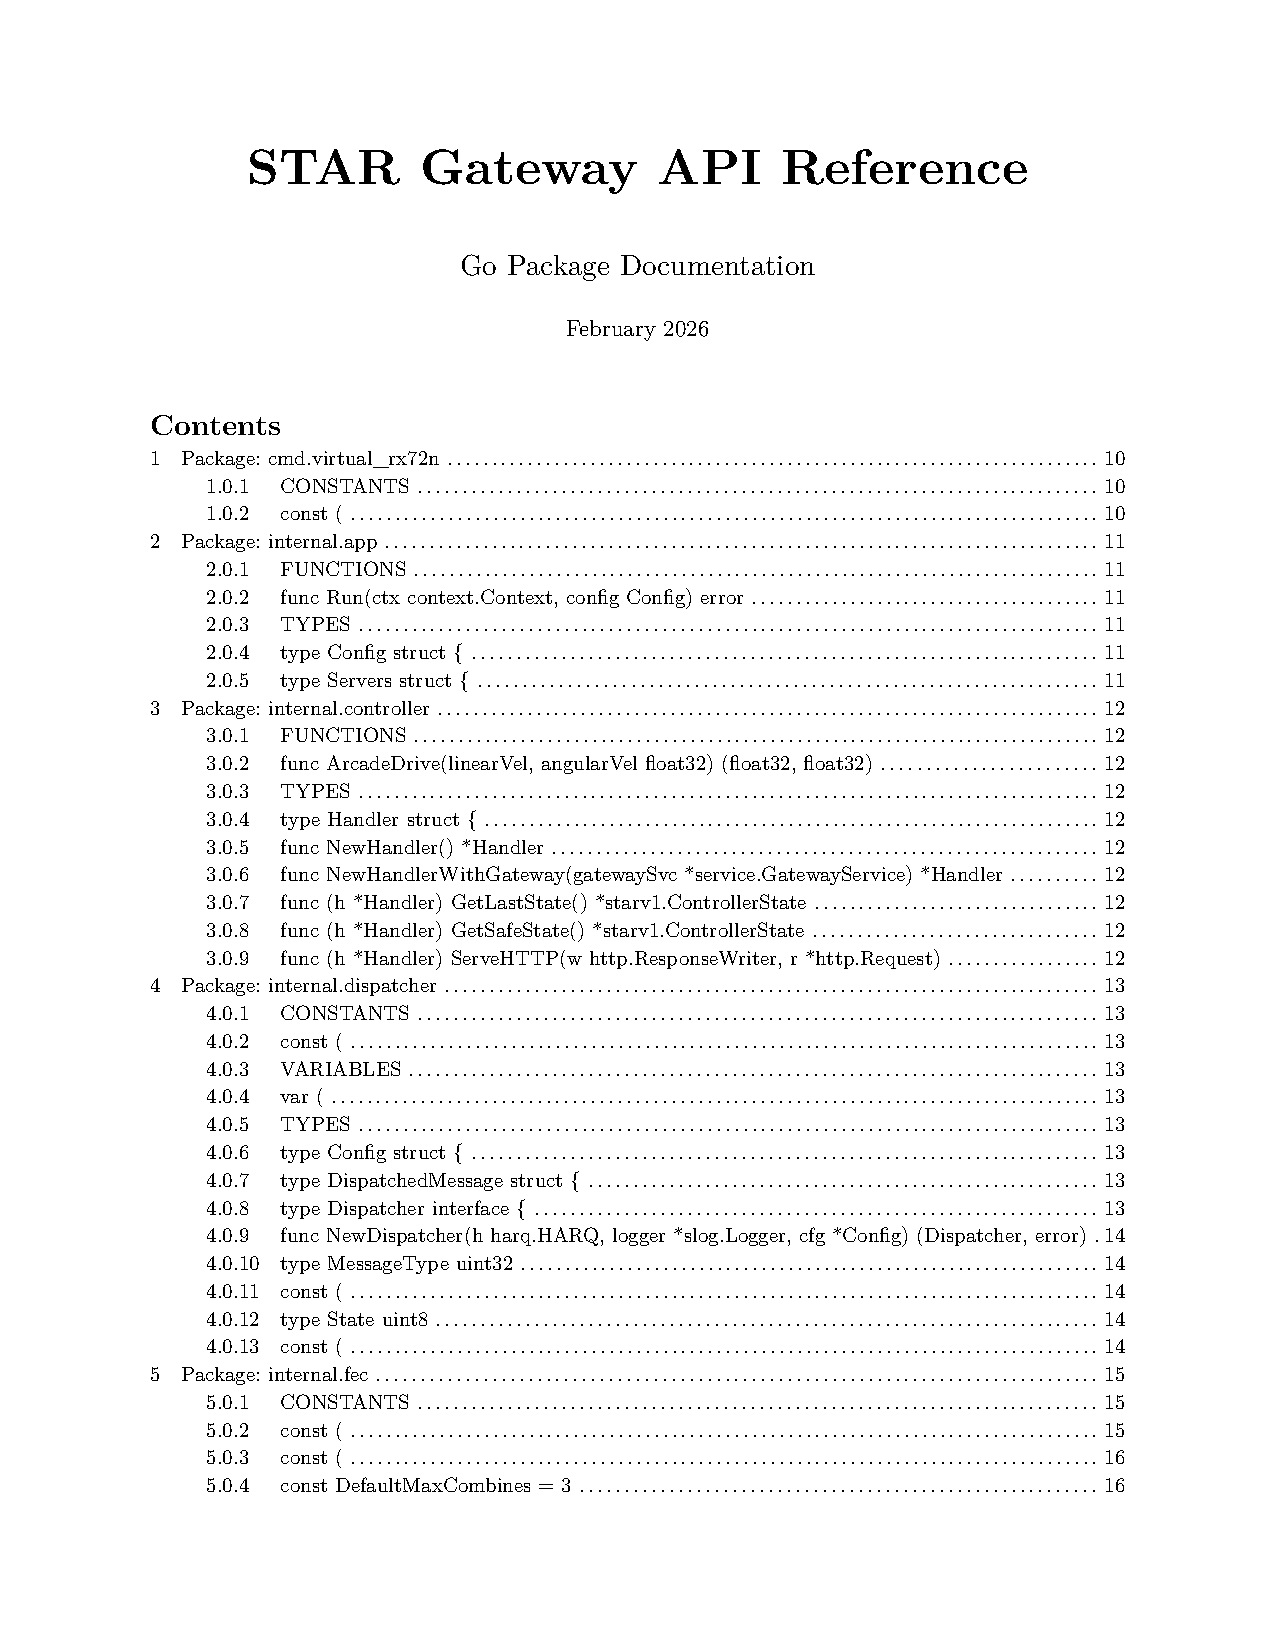
\includepdf[pages=-, pagecommand={\thispagestyle{fancy}}, fitpaper=false, width=\textwidth]{star_gateway_api.pdf}

% =============================================================================
% PART VI: API REFERENCE - ROS2 (C++)
% =============================================================================
\part{API Reference -- ROS2 (C++)}

\newpage
\section*{ROS2 API Reference}
\addcontentsline{toc}{section}{ROS2 API Reference}

This section contains the complete auto-generated API reference for the
STAR ROS2 packages. Generated from C++ source code comments using Doxygen.

\vspace{1em}
\noindent\textbf{Source:} \texttt{star-ros2/src/}\\
\textbf{Language:} C++17\\
\textbf{Framework:} ROS2 Humble\\
\textbf{Generator:} Doxygen \texttt{1.16.1}

\newpage
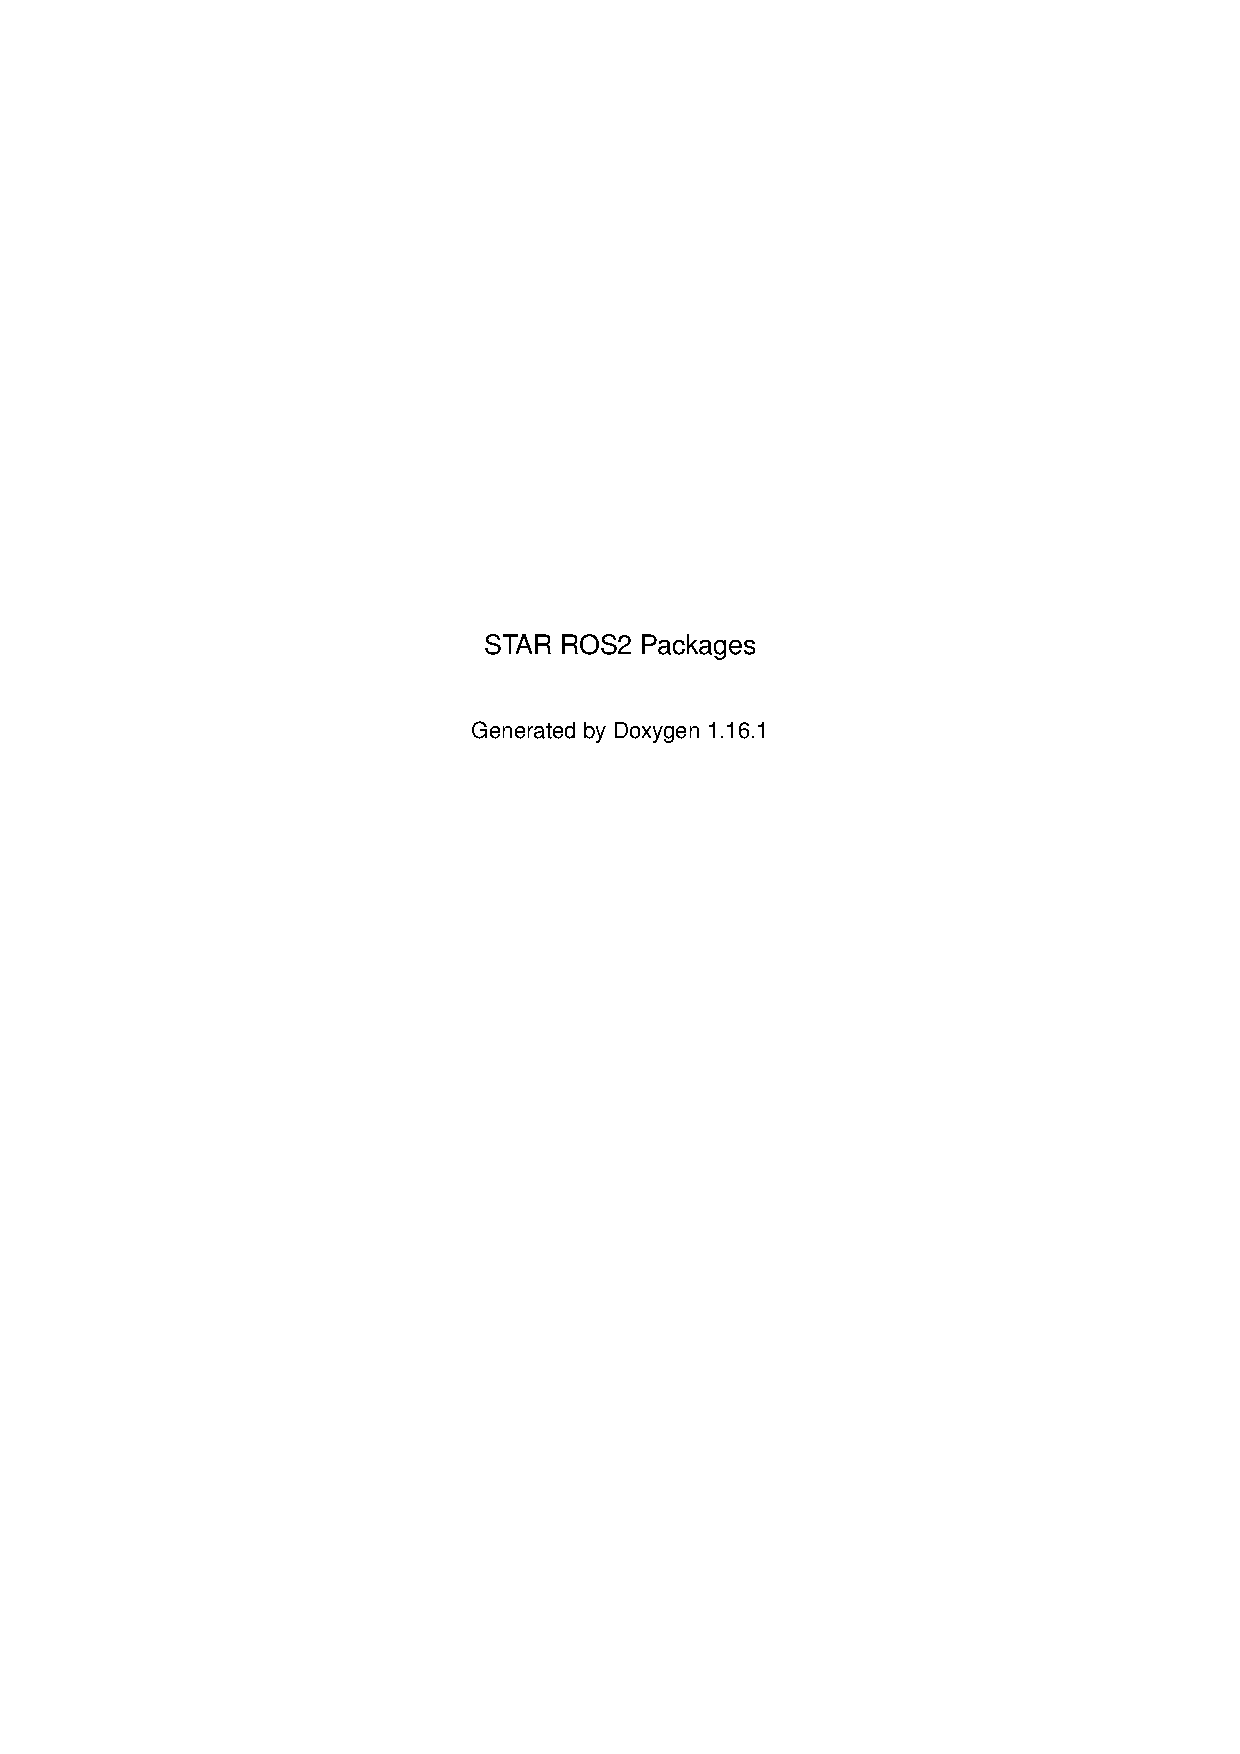
\includepdf[pages=-, pagecommand={\thispagestyle{fancy}}, fitpaper=false, width=\textwidth]{star_ros2_api.pdf}

\end{document}
